\documentclass{amsart}

\usepackage[T1]{fontenc}
\usepackage{lmodern}
\usepackage{mathtools}
\usepackage{booktabs}
\usepackage{hyperref}
\usepackage{graphicx}
\usepackage{microtype}
\usepackage{tikz}
\usetikzlibrary{positioning,decorations.pathreplacing,arrows.meta,calc,3d}

% ---------- theorem styles ----------
\newtheorem{theorem}{Theorem}[section]
\newtheorem{proposition}[theorem]{Proposition}
\newtheorem{corollary}[theorem]{Corollary}
\newtheorem{lemma}[theorem]{Lemma}
\theoremstyle{definition}
\newtheorem{definition}[theorem]{Definition}
\theoremstyle{remark}
\newtheorem{remark}[theorem]{Remark}
\newtheorem{example}[theorem]{Example}

% ---------- notation ----------
\newcommand{\R}{\mathbb{R}}
\newcommand{\Z}{\mathbb{Z}}
\newcommand{\N}{\mathbb{N}}
\newcommand{\Q}{\mathbb{Q}}
\DeclareMathOperator{\sgn}{sgn}
\DeclareMathOperator{\rank}{rank}
\newcommand{\dH}{\dim_{\mathrm{H}}}
\DeclareMathOperator{\Pell}{Pell}
\title{Disk-Like Self-Similar Tiles with High Boundary Dimension}

\author{Dmitry Mekhontsev}
\address{Novosibirsk State University, Novosibirsk, Russia}
\email{mekhontsev@gmail.com}
\subjclass[2020]{28A80 (primary), 52C20, 37C70 (secondary)}
\keywords{Self-similar tile, boundary dimension, Hausdorff dimension,
  neighbor graph, disk-like tile}
\date{\today}

% --------------------------------------------------------------------------
\begin{document}

\begin{abstract}
For every $d \ge 1$ and every $n \ge 3$ we construct a
self-similar tile $C_n^{(d)} \subset \R^d$ generated by
$n$~contractions of ratio~$n^{-1/d}$, with the following
properties.

\smallskip
\emph{Uniform neighbor structure.}  The number of boundary
components $p(d)$ of the neighbor graph is independent of~$n$ and
satisfies the Pell-type recurrence
\[
  p(d) \;=\; 2\,p(d{-}1) \;+\; p(d{-}2) \;+\; 2,
\]
with $p(0)=0$ and $p(1)=2$.

\smallskip
\emph{Asymptotic boundary dimension.}  Using the decomposition of the
boundary substitution matrix $M_n^{(d)} = n A^{(d)} + B^{(d)}$ and a
Sherman--Morrison--Woodbury identity for the $M_{--}$ block, we prove
\[
  \lambda_n^{(d)} \;=\; n \;-\; \tfrac{2d}{n} \;+\; O(n^{-2}),
  \qquad
  d - \dH\bigl(\partial C_n^{(d)}\bigr)
    \;\sim\; \frac{2 d^2}{n^2 \log n},
\]
so $\dH(\partial C_n^{(d)}) \to d$ as $n \to \infty$ while the
neighbor graph complexity remains bounded.

\smallskip
\emph{One-dimensional extremality.}  In dimension one, among all
complete-residue systems of scale~$n$, every irreducible two-state
principal subblock of the boundary substitution matrix has spectral
radius at most that of the comb.  Thus $C_n^{(1)}$ is extremal whenever
the boundary dimension is carried by a closed two-state component, with
rigid equality up to affine conjugacy, global reflection, and relabeling
of the maps.

\smallskip
\emph{Topology.}  The tiles are connected for all $d \ge 2$, and in
the plane each $C_n^{(2)}$ is disk-like.  Ball-likeness in dimensions
$d \ge 3$ remains open; we conjecture it holds for every $n \ge 3$.
\end{abstract}

\maketitle

% --------------------------------------------------------------------------
\section{Introduction}
\label{sec:intro}

A \emph{self-similar tile} is a compact set $A \subset \R^d$ with
non-empty interior satisfying
\[
  A = \bigcup_{i=0}^{N-1} f_i(A),
\]
where the $f_i$ are contractive similarities~\cite{hutchinson} and the union is
measure-disjoint (the \emph{Open Set Condition}, hereafter OSC).
Such tiles arise naturally in the study of
self-affine lattice tilings~\cite{lagarias-wang}.
The \emph{boundary} $\partial A$ is a compact fractal set whose
Hausdorff dimension $s = \dH(\partial A)$ satisfies
$d - 1 \le s < d$
(see~\cite{falconer} for background on Hausdorff dimension).

\textbf{Achieving $\dH(\partial A)$ close to $d$ is easy in principle.}
Keesling~\cite{keesling} proved that $\dH(\partial A) < d$ for every
self-similar tile in~$\R^d$ and gave examples in every dimension
showing that $\dH(\partial A)$ can be arbitrarily close to~$d$
(see also Duvall, Keesling and Strichartz~\cite{duvall-keesling-strichartz}
for explicit calculations of boundary dimensions).  These results
show that the upper-dimensional envelope is attainable; the question
left open here is whether it can be attained while the neighbor graph
complexity stays bounded for each fixed ambient dimension.

\textbf{The disk-like constraint is much more restrictive.}
High boundary dimension corresponds to extreme geometric roughness of
$\partial A$, and planar tiles with large $\dH(\partial A)$ are generically
non-disk-like (e.g., the L{\'e}vy~C curve with
$\dH(\partial A) \approx 1.934$ is not a topological disk).
Achieving $\dH(\partial A)$ close to~$d$ while maintaining the
disk-like (or ball-like) property and bounded graph complexity is therefore a much
harder problem.

The natural question arises: \emph{can $\dH(\partial A)$ approach~$d$
with a bounded number of boundary components and the appropriate
disk-like or ball-like topology?}

\textbf{Main result (informal).}
For every $d \ge 1$ and every $n \ge 3$ there is a self-similar
tile $C_n^{(d)} \subset \R^d$, defined by $n$~contractions of ratio
$n^{-1/d}$ (Definition~\ref{def:comb},
Sections~\ref{sec:higherdim}--\ref{sec:asymp-arbitrary-d}),
such that:
\begin{itemize}
\item[(a)] \emph{Bounded graph complexity:} the neighbor graph of
  $C_n^{(d)}$ has exactly $p(d) = H_{d+1} - 1$ boundary
  components, independent of~$n$, where $H_{d+1}$ is the
  $(d{+}1)$-st half-companion Pell number (OEIS~A001333);
  equivalently $p(d)$ satisfies the Pell-type recurrence
  $p(d) = 2p(d{-}1) + p(d{-}2) + 2$ with $p(0)=0$, $p(1)=2$
  (Corollary~\ref{cor:pell}).
\item[(b)] \emph{Boundary dimension tends to~$d$:}
  \[
    \lambda_n^{(d)} = n - \tfrac{2d}{n} + O(n^{-2}),
    \qquad
    d - \dH\!\bigl(\partial C_n^{(d)}\bigr)
      \sim \frac{2 d^2}{n^2 \log n}
    \qquad (n \to \infty),
  \]
  where $\lambda_n^{(d)}$ is the Perron eigenvalue of the boundary
  substitution matrix $M_n^{(d)}$
  (Theorem~\ref{thm:asymp-d-forward}).  In the closed-form case $d = 1$
  (Section~\ref{ssec:d1}), $\lambda_n^{(1)}$ is the dominant root
  of $x^2 - (n{-}1)x - (n{-}2)$; for $d = 2$,
  $\lambda_n^{(2)}$ is the dominant root of the explicit quartic
  \[
    p_n(x) = x^4 - (n{-}1)x^3 - 2x^2 - (n{-}1)(n{-}4)x + n(n{-}2)
  \]
  (Theorem~\ref{thm:dim}).  In arbitrary dimension the
  asymptotics are proved from an $n$-independent decomposition
  of the boundary substitution matrix,
  $M_n^{(d)} = n A^{(d)} + B^{(d)}$, together with a
  Sherman--Morrison--Woodbury identity for the $M_{--}$ block.
  This perturbation argument identifies the universal coefficient
  $-2d$ (Theorem~\ref{thm:asymp-d}).
\item[(c)] \emph{One-dimensional extremality:} among all
  complete-residue one-dimensional systems of scale~$n$, every
  irreducible two-state principal subblock of the boundary substitution
  matrix has spectral radius at most the comb value.  Hence, when a
  closed two-state component carries the boundary
  dimension, the one-dimensional tile $C_n^{(1)}$
  constructed here is extremal, and equality forces this system up to
  the natural affine and orientation symmetries
  (Theorem~\ref{thm:d1-two-neighbor-extremal}).
\item[(d)] \emph{Disk-likeness in the plane ($d = 2$):}
  $C_n^{(2)}$ is homeomorphic to the closed disk, and the tiling
  has the combinatorial type of the regular hexagonal tiling: each
  tile has $6$~edge neighbors and $6$~triple points of valence~$3$
  (Theorem~\ref{thm:disklike}, Remark~\ref{rem:topology}).  In
  dimension $d \ge 3$ ball-likeness remains open; we conjecture
  that $C_n^{(d)}$ is homeomorphic to the closed $d$-ball for
  every $n \ge 3$.
\item[(e)] \emph{Connectedness and full-dimensional piece contacts:}
  every non-empty intersection between distinct level-one pieces
  $f_i(C_n^{(d)})$ has Hausdorff dimension
  $\dH(\partial C_n^{(d)})$, for every $d \ge 1$ and $n \ge 3$
  (Proposition~\ref{prop:face-to-face}).  For $d \ge 2$, the
  consecutive spine contacts and the tooth-pair contact are non-empty
  and form a connected chain, so $C_n^{(d)}$ is connected
  (Proposition~\ref{prop:connected}).  At $d = 1$, the consecutive
  spine contacts are absent and $C_n^{(1)}$ is a Guthrie--Nymann
  cantorval~\cite{guthrie-nymann}, hence not connected; nevertheless
  its non-empty level-one contacts still have full boundary dimension.
\item[(f)] \emph{Periodic crystallographic tiling with
  uniform-dimension contacts:} for every $d \ge 1$ and every
  $n \ge 3$, $C_n^{(d)}$ tiles $\R^d$ periodically in the
  crystallographic sense: the tiling consists of translates of
  $C_n^{(d)}$ and of its central reflection $-C_n^{(d)}$, over the
  standard lattice.  Equivalently, it is the orbit tiling under the
  group generated by $\Z^d$-translations and the map $x\mapsto -x$.
  Every non-empty intersection of distinct tiles in this periodic
  two-orientation tiling has Hausdorff dimension equal to
  $\dH(\partial C_n^{(d)})$
  (Proposition~\ref{prop:face-to-face}).  In particular the
  tiling has no point or lower-dimensional contacts; in $d = 2$
  this realises the combinatorial type of the regular hexagonal
  tiling \textup{(}item (d) above\textup{)}, and in $d \ge 3$ it
  rules out, unconditionally, all contacts of codimension
  $\ge 2$.
\end{itemize}
Except for the ball-likeness question in dimensions $d \ge 3$, which
is stated here as a conjecture, the assertions above are proved for all
dimensions for which they are stated.  The proofs reduce the problem to
an explicit analysis of the refinement equation, together with standard
criteria for the OSC, connectedness, and disk-likeness; the case $d=1$
is treated separately where its topology differs from the higher-
dimensional case.

\textbf{Discovery.}
The construction grew out of experiments with IFStile~\cite{ifstile}.
In an initial search through a planar five-map subfamily, one candidate
stood out: it had a large boundary dimension, a very small neighbor
graph, and a picture that strongly suggested a disk-like tile.  This
comb-shaped example was the starting point.  Its geometry made it
natural to ask whether the visible pattern could be extended from five
maps to an arbitrary number of maps.  After a few experiments with the
affine maps, the planar comb family emerged.  Further IFStile checks for
many values of~$n$ showed the same qualitative behaviour: the number of
neighbors stayed constant, while the boundary dimension rapidly
approached~$2$.  These observations led to the planar proofs of
disk-likeness, the $n$-independent neighbor graph, and the asymptotic
dimension formula in Section~\ref{sec:d2}.

The higher-dimensional family was found next.  In dimension~$3$ the main
experimental question was how far to shift the new tooth coordinate.
Searches over several shifts and several values of~$n$ singled out the
same value $2n{-}3$ that already occurs in the planar construction: it
again produced a small neighbor graph whose size did not depend on~$n$.
Tests in dimensions $d>3$ showed the same stable behaviour when each new
coordinate was added with this shift.  At the same time, the number of
neighbors as a function of~$d$ revealed the Pell-type pattern
$H_{d+1}-1$, giving further evidence that the construction was not an
accident.  The one-dimensional member was examined last; it follows the
same boundary-substitution mechanism, apart from the expected failure of
connectedness.  The analytic part of the paper grew from this sequence
of experiments, extending the planar structure to all~$n$ and~$d$ in
Sections~\ref{sec:higherdim}--\ref{sec:asymp-arbitrary-d}.

\subsection*{Related work}

The comb family sits at the intersection of three strands of the
literature.

\emph{Topology and disk-likeness of self-similar tiles.}
General criteria for a planar self-affine tile to be homeomorphic to
a disk were developed by Bandt and Wang~\cite{bandt-wang}, with
further refinements by Leung and Lau~\cite{leung-lau} and Ngai and
Tang~\cite{ngai-tang}.  For the planar comb we use the criterion of
Loridant, Luo and Thuswaldner~\cite{loridant-luo-thuswaldner} for
crystallographic tiles, phrased in terms of neighbor and boundary-piece
graphs.  A broader survey of topological properties of tiles arising
from number systems is given by Akiyama and
Thuswaldner~\cite{akiyama-thuswaldner}.

\emph{Boundary dimension.}
The computation of $\dH(\partial A)$ for a self-similar tile reduces
to the spectral radius of a graph-directed substitution
matrix~\cite{mauldin-williams}, whose construction via the neighbor
graph was systematised by Scheicher and
Thuswaldner~\cite{scheicher-thuswaldner}; explicit calculations for
specific families appear in Duvall, Keesling and
Strichartz~\cite{duvall-keesling-strichartz}.  Keesling's
bound~\cite{keesling} $\dH(\partial A) < d$ for tiles in~$\R^d$
together with his examples approaching this bound provide the
upper-dimension envelope within which our construction lives.

\emph{Self-affine tilings and separation.}
The broader setting of self-affine lattice tilings is due to
Bandt~\cite{bandt1991} and Lagarias and Wang~\cite{lagarias-wang};
the Open Set Condition and its weakenings are studied by Lau and
Ngai~\cite{lau-ngai}.  The comb IFS is self-similar in the strict
sense (equal contraction ratios, orthogonal linear parts), so OSC and
the classical Moran formula apply directly.  Because the digit maps use
both orientations, the natural tiling is a crystallographic
two-orientation tiling rather than a pure translate tiling; this is the
setting in which the neighbor analysis is carried out below.

\subsection*{Position of the comb family}

The comb family is close to, but not contained in, two common sources of
examples.  \emph{Number-system tiles}~\cite{akiyama-thuswaldner,
lagarias-wang}, including the classical twindragon, typically use a fixed
expanding matrix together with a digit set forming a complete residue
system in an algebraic lattice.  A second source is provided by highly
symmetric planar examples, such as the terdragon and related cyclic
constructions, where the digits are arranged with substantial rotational
or reflectional symmetry and the boundary substitutions reflect this
symmetry.

The comb construction uses a different mechanism.  Its $n{-}1$
collinear ``spine'' maps have linear part~$+I$, while one transverse
``tooth'' map has linear part~$-I$ and offset $2n{-}3$.  This
mixed-orientation, parameter-dependent geometry is asymmetric but still
rigid enough to leave a neighbor graph whose size is independent of~$n$.
It is this combination that the paper exploits: small boundary
substitution complexity, disk-like planar topology, and a Perron root
approaching the full value~$n$.  In higher dimensions the same tooth
offset produces the Pell-type growth of the neighbor count while the
boundary dimension tends to the ambient dimension.

% --------------------------------------------------------------------------
\section{The Comb Family}
\label{sec:comb}

\subsection{Definition via companion matrix}

For integers $d \ge 1$ and $n \ge 2$, let
$g = g_{d,n} \in \Z^{d \times d}$
be the companion matrix of the monic polynomial $x^d - n$.
Its eigenvalues are
$n^{1/d}\,\zeta_d^k$ for $k = 0, \ldots, d{-}1$
(where $\zeta_d = e^{2\pi i/d}$), all of common modulus $n^{1/d}$.
For $d = 2$, $g = \bigl(\begin{smallmatrix}0 & n \\ 1 & 0\end{smallmatrix}\bigr)$
has eigenvalues $\pm\sqrt n$; for $d = 1$, $g = n$ is scalar.

\begin{remark}[Self-similarity]
\label{rem:jordan-similarity}
Since all eigenvalues of~$g$ have equal modulus $n^{1/d}$, the
matrix~$g$ is similar over~$\R$ (via its real Jordan basis) to a
Euclidean similarity of ratio $n^{1/d}$.
Consequently, the IFS of Definition~\ref{def:comb-d} below, although
written with integer coefficients in the standard basis of~$\Z^d$,
becomes \emph{self-similar} (in the strict sense: every contraction
is a Euclidean similarity of common ratio $n^{-1/d}$) in the real
Jordan basis of~$g$.
This holds for every $d \ge 1$ and $n \ge 2$.
\end{remark}

\begin{definition}[Comb IFS]\label{def:comb-d}\label{def:comb}
For $d \ge 1$ and $n \ge 2$, the \emph{$d$-dimensional comb IFS with
parameter~$n$} consists of $n$ digit maps acting on~$\R^d$:
\begin{equation}\label{eq:comb-maps}
\begin{aligned}
  h_j(x) &= x + j(n{-}1)\,e_1,
    &\quad j &= 0, \ldots, n{-}2, \\[2pt]
  h_{n-1}(x) &= -x + \bigl(n^2{-}n{-}1,\;
    \underbrace{2n{-}3, \ldots, 2n{-}3}_{d-1}\bigr),
\end{aligned}
\end{equation}
where $e_1 = (1, 0, \ldots, 0)$
(for $d = 1$ the underbraced block is empty,
so $h_{n-1}(x) = -x + (n^2{-}n{-}1)$),
with attractor
\begin{equation}\label{eq:attractor}
  C_n^{(d)} = g^{-1}\bigl(h_0(C_n^{(d)}) \cup \cdots \cup h_{n-1}(C_n^{(d)})\bigr).
\end{equation}
All digits are integer vectors.  The map $h_{n-1}$ includes a central
reflection $x \mapsto -x$.
The case $n = 2$ degenerates to a parallelepiped in every dimension
$d \ge 1$ (a non-fractal disk-like tile); the structural results below
assume $n \ge 3$.
\end{definition}

\begin{figure}[ht]
\centering
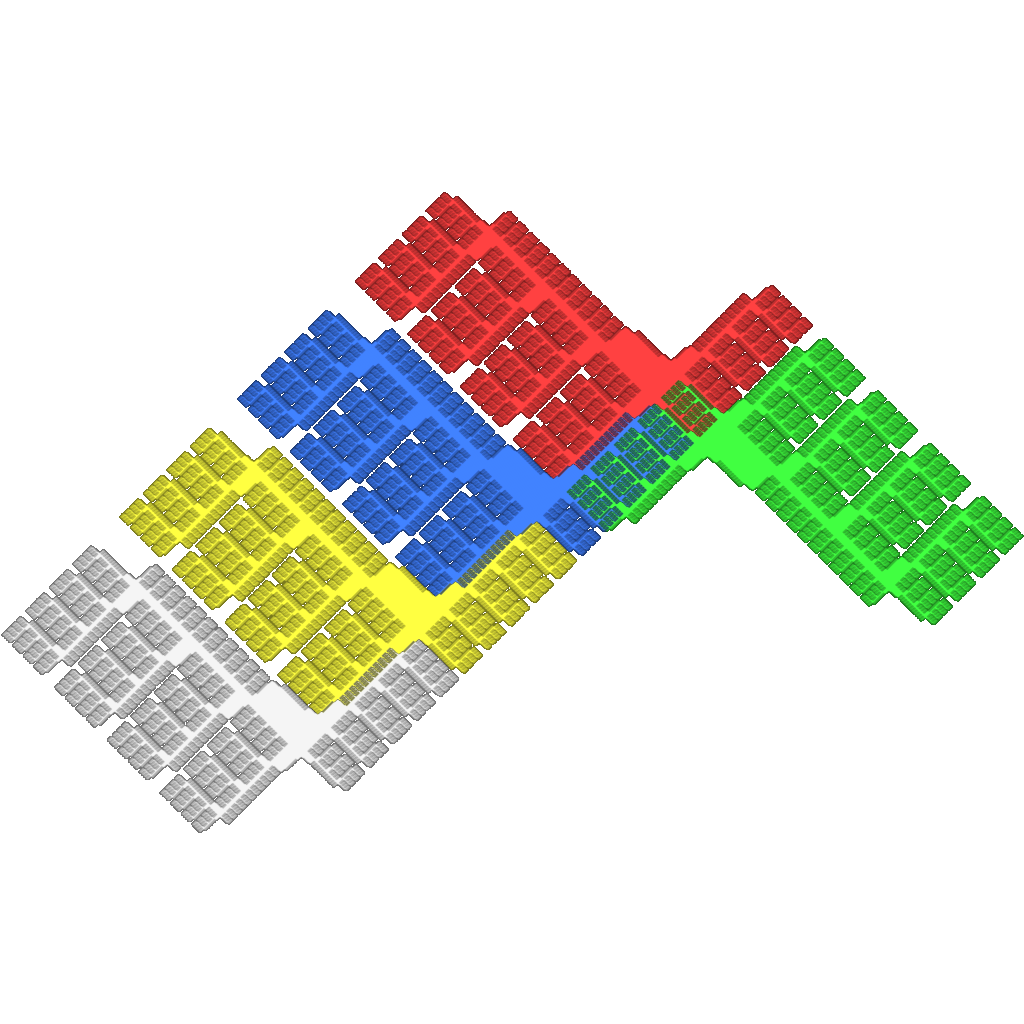
\includegraphics[width=0.65\textwidth]{comb-tile-n5.png}
\caption{The comb tile $C_5$ ($n = 5$, five maps).  Each first-level
  piece $f_j(C_5)$ is shown in a distinct colour: the four spine pieces
  $f_0, \ldots, f_3$ tile the lower-left staircase, while the single
  tooth piece $f_4$ (with central reflection) extends to the upper right.}
\label{fig:comb-tile}
\end{figure}

\begin{figure}[ht]
\centering
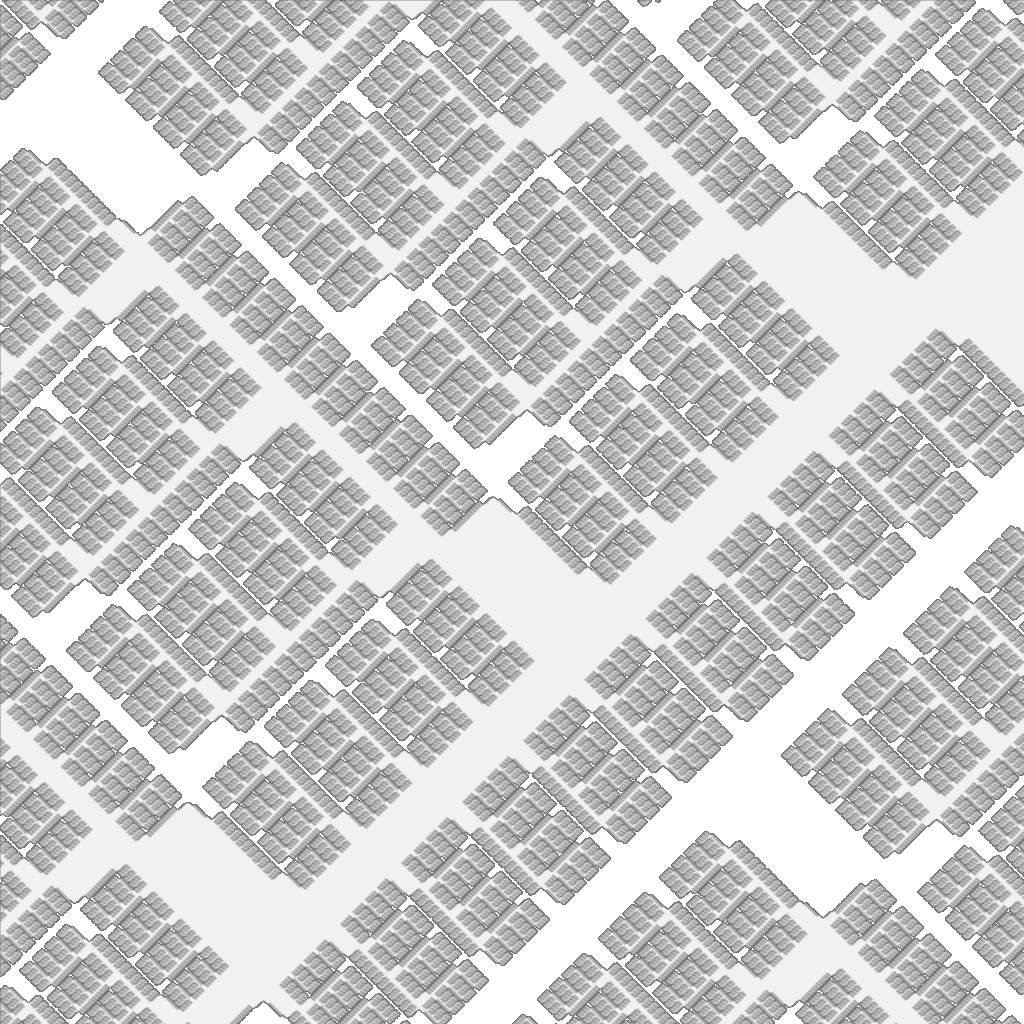
\includegraphics[width=0.55\textwidth]{comb-tile-n5-zoom.png}
\caption{Magnified fragment of the boundary $\partial C_5$.
  The boundary is a Jordan curve ($C_5$ is disk-like by
  Theorem~\ref{thm:disklike}), yet its Hausdorff dimension is
  $\dH(\partial C_5) \approx 1.863$ --- visibly close to
  space-filling.}
\label{fig:comb-zoom}
\end{figure}

\begin{figure}[ht]
\centering
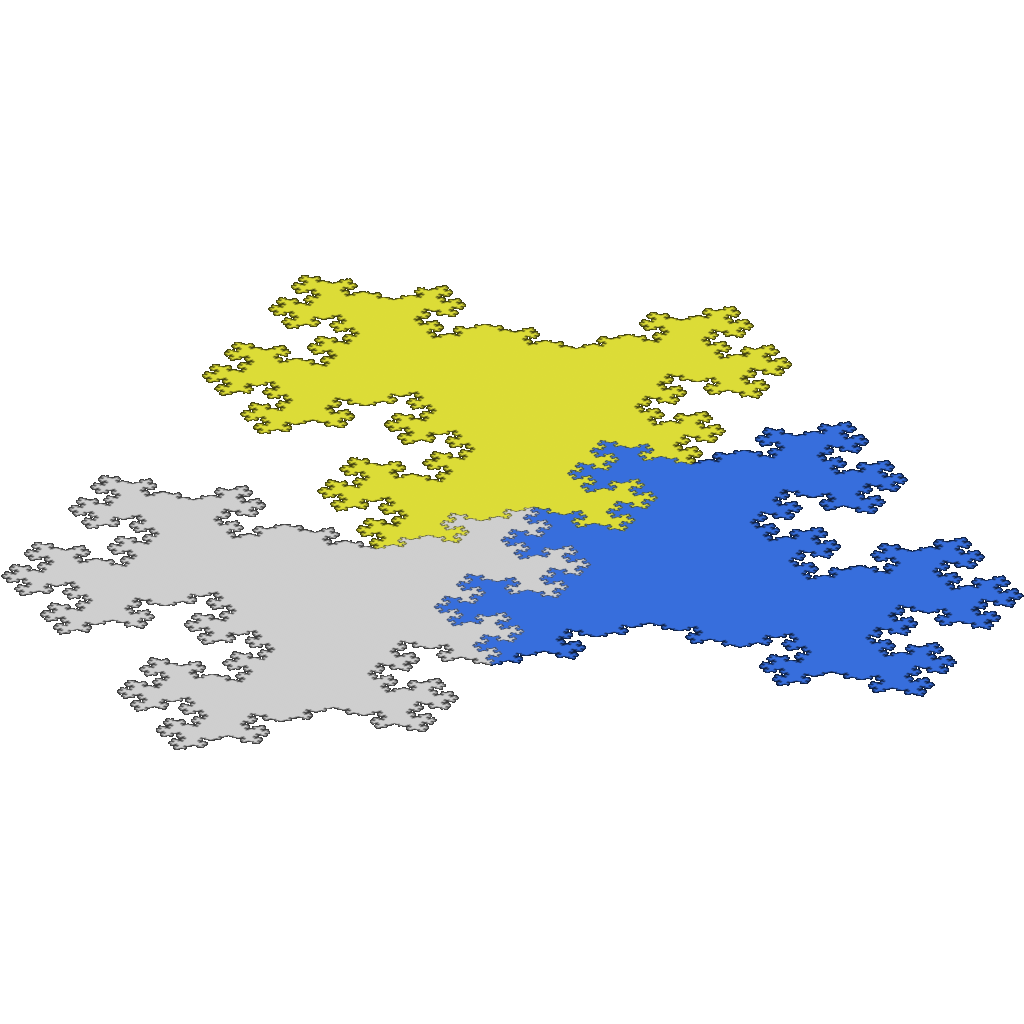
\includegraphics[width=0.48\textwidth]{comb-tile-n3.png}\hfill
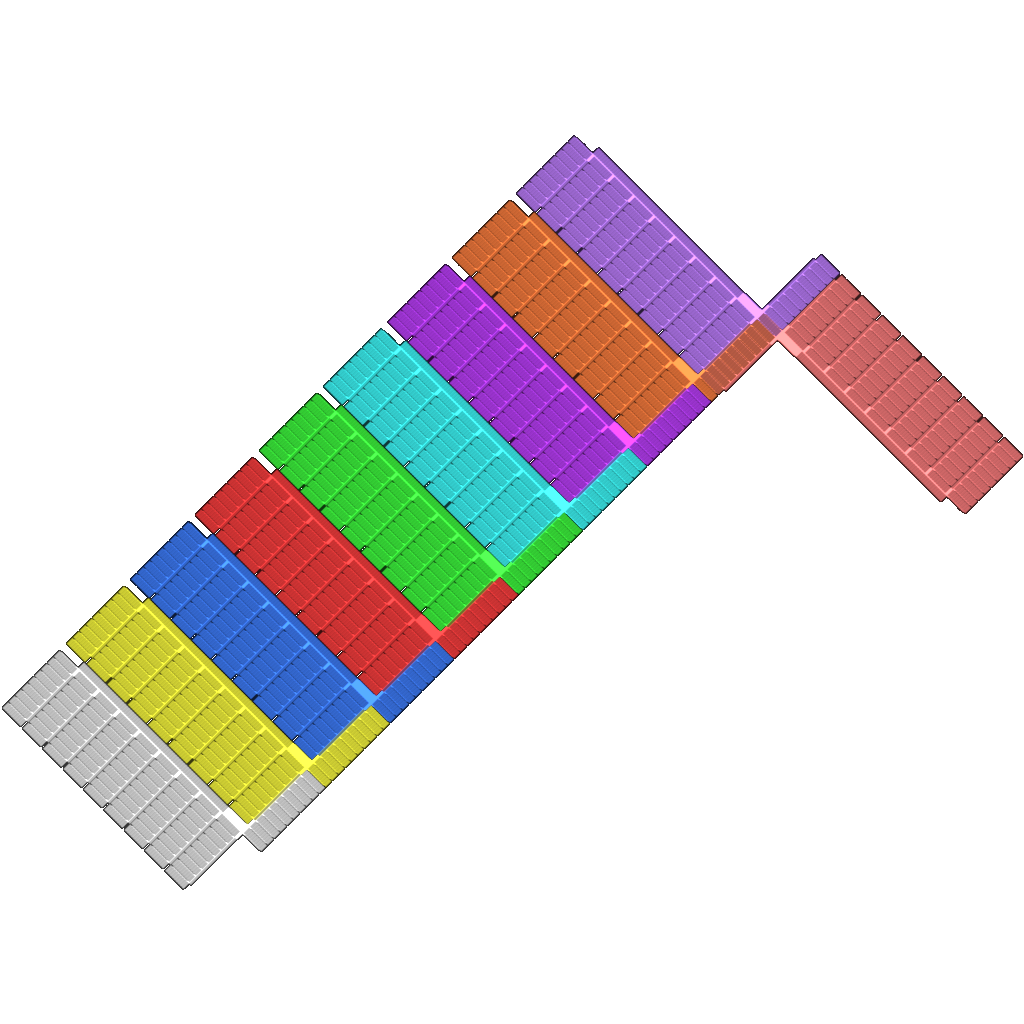
\includegraphics[width=0.48\textwidth]{comb-tile-n10.png}
\caption{Boundary complexity progression.
  \emph{Left:} the comb tile $C_3$ ($n = 3$, three maps),
  $\dH(\partial C_3) \approx 1.453$ --- the boundary is visibly
  fractal.
  \emph{Right:} the comb tile $C_{10}$ ($n = 10$, ten maps),
  $\dH(\partial C_{10}) \approx 1.973$ --- the boundary is nearly
  space-filling, and the tile is almost polygonal.
  Compare with~$C_5$ in Figure~\ref{fig:comb-tile}.}
\label{fig:comb-progression}
\end{figure}

Each contraction $f_j = g^{-1} \circ h_j$ is an affine similarity with
linear part $\pm g^{-1}$, and (in the real Jordan basis of~$g$,
Remark~\ref{rem:jordan-similarity}) common contraction ratio
$n^{-1/d}$.

\begin{remark}[Digit set geometry]
\label{rem:digits}
The first $n{-}1$ digits $h_0, \ldots, h_{n-2}$ are pure translations
along the first coordinate axis, with displacements
$0,\, n{-}1,\, 2(n{-}1),\, \ldots,\, (n{-}2)(n{-}1)$.  These form the
\emph{spine} of the comb.
The single map $h_{n-1}$, which includes a central reflection, has an
off-axis translation component and forms the \emph{tooth} of the comb.
This asymmetric digit geometry --- one outlier map among $n{-}1$ collinear
ones --- is the structural source of the small neighbor graph size
(see Subsection~\ref{sec:osc}).
The name \emph{comb} reflects the first-level subdivision visible in
Figure~\ref{fig:comb-tile}: the $n{-}1$ spine pieces form a row of
teeth, while the single reflected piece extends sideways like a handle.
\end{remark}

\subsection{Basic properties}

Since all $n$ maps share the contraction ratio $r = n^{-1/d}$, the
Moran formula gives $\dH(C_n^{(d)}) = d$ provided the OSC holds.
The OSC and the tiling property are established in
Proposition~\ref{prop:bandt-sym} and Corollary~\ref{cor:comb-tile}
below, by the same Bandt-type residue argument that works in every
dimension.  Proposition~\ref{prop:tiling} records the explicit form of
the resulting two-orientation crystallographic tiling.

To verify the tiling property rigorously, we reformulate
{\cite[Theorem~2]{bandt1991}} in a form where the residue condition
is identical to the purely translational case (Theorem~1 ibid.).

\begin{proposition}[Tiling criterion with symmetries,
  after {\cite[Theorem~2]{bandt1991}}]
\label{prop:bandt-sym}
Let $L \in \Z^{d \times d}$ be expanding with $m = |\det L|$,
and let $S$ be a finite group of integer matrices with
$\det s = \pm 1$ for every $s \in S$, such that $L$ normalizes~$S$
(i.e.\ $LSL^{-1} = S$).
Given $s_1,\ldots,s_m \in S$ and
\emph{digit vectors} $h_1,\ldots,h_m \in \Z^d$,
define the attractor~$A$ by
\begin{equation}\label{eq:ifs-sym}
  A \;=\; \bigcup_{i=1}^{m} L^{-1}\,s_i(A + h_i).
\end{equation}
If $\{h_1,\ldots,h_m\}$ is a complete residue system
for $\Z^d / L\Z^d$, then $A$ has nonempty interior,
the open set condition holds with
$V = \operatorname{int}(A)$, and $\dH(A) = d$.
\end{proposition}

\begin{proof}
Set $y_i = s_i\,h_i$ and consider the contractions
$f_i(x) = s_i\,L^{-1}(x) + y_i$, which are in the
form of Theorem~2 in~\cite{bandt1991}.
The lattice condition of that theorem requires
\[
  \Z^d = \bigcup_{i=1}^{m} s_i^{-1}\bigl(y_i + L\Z^d\bigr).
\]
Since $LSL^{-1} = S$, we have
$L^{-1}s_i^{-1}L \in S \subset \mathrm{GL}(d,\Z)$, so
$s_i^{-1}\,L\Z^d = L(L^{-1}s_i^{-1}L)\Z^d = L\Z^d$, and
\[
  s_i^{-1}(y_i + L\Z^d)
  = s_i^{-1}y_i + L\Z^d
  = h_i + L\Z^d,
\]
and the condition reduces to $\{h_i\}$ being a complete
residue system for~$\Z^d/L\Z^d$ --- our hypothesis.

Theorem~2 of~\cite{bandt1991} now yields a unique attractor
$\hat{A} = \bigcup_i f_i(\hat{A})$ with nonempty interior and
$\dH(\hat{A}) = d$.
Setting $A = L^{-1}\hat{A}$, we verify~\eqref{eq:ifs-sym}:
\[
  L^{-1}\,s_i(A + h_i)
  = L^{-1}\bigl(s_i\,L^{-1}\hat{A} + s_i\,h_i\bigr)
  = L^{-1}\,f_i(\hat{A}),
\]
so $\bigcup L^{-1}\,s_i(A + h_i)
  = L^{-1}\hat{A} = A$.
Since $L^{-1}$ is a linear bijection,
$\operatorname{int}(A) \ne \emptyset$ and $\dH(A) = d$.
The open set condition
for~\eqref{eq:ifs-sym} holds with
$V = L^{-1}(\operatorname{int}\hat{A}) = \operatorname{int}(A)$.
\end{proof}

\begin{corollary}[Comb tile]\label{cor:comb-tile}
For every $d \ge 1$ and $n \ge 2$, the attractor $C_n^{(d)}$
of Definition~\ref{def:comb-d} tiles~$\R^d$, satisfies the OSC,
and $\dH(C_n^{(d)}) = d$.
\end{corollary}

\begin{proof}
The symmetry group $S = \{I,-I\}$ is central in $\mathrm{GL}(d,\Z)$,
so the companion matrix $g$ normalizes~$S$.
The digit maps of Definition~\ref{def:comb-d} have the form
$h_j(x) = s_j\,x + d_j$ with $s_j = I$ for $j < n{-}1$
and $s_{n-1} = -I$.
In the notation of~\eqref{eq:ifs-sym}, with $L = g$, the digit vectors are
$v_j = s_j^{-1}d_j$:
\[
  v_j = j(n{-}1)\,e_1 \;\;(j = 0,\ldots,n{-}2),
  \qquad
  v_{n-1} = -d_{n-1}.
\]
The companion matrix $g$ satisfies $|\det g| = n$,
and $g\Z^d$ is spanned by $\{e_2,\ldots,e_d,\,ne_1\}$
(since $ge_k = e_{k+1}$ for $k < d$ and $ge_d = ne_1$),
so $\Z^d/g\Z^d \cong \Z/n\Z$ via the first coordinate modulo~$n$.
The first coordinates of the digit vectors modulo~$n$ are:
$j(n{-}1) \equiv -j$ for $j = 0,\ldots,n{-}2$,
and $-(n^2{-}n{-}1) \equiv 1$ for $j = n{-}1$.
Thus the residues are
$\{0, n{-}1, n{-}2, \ldots, 2, 1\} = \{0,1,\ldots,n{-}1\}$,
a complete system.
The result follows from Proposition~\ref{prop:bandt-sym}.
\end{proof}

\begin{proposition}[Self-replicating tiling]\label{prop:tiling}
For every $d \ge 1$ and $n \ge 3$, $C_n^{(d)}$ is an $n$-rep tile
in the two-orientation crystallographic sense: $\R^d$ is tiled by
copies of $C_n^{(d)}$ and its central reflection $-C_n^{(d)}$:
\[
  \R^d = \bigcup_{v \in \Z^d} (C_n^{(d)} + v)
         \;\cup\; \bigcup_{w \in \Z^d} (-C_n^{(d)} + w),
\]
with the union measure-disjoint.
\end{proposition}

\begin{proof}
Corollary~\ref{cor:comb-tile} applies Proposition~\ref{prop:bandt-sym}
with the symmetry group $S = \{I,-I\}$.  The associated orbit tiling
therefore consists exactly of $\Z^d$-translates of $C_n^{(d)}$ and
of $-C_n^{(d)}$.  The measure-disjointness is the OSC from
Corollary~\ref{cor:comb-tile}.
\end{proof}

% [Paragraph on real eigenvalues of g dropped: superseded by
%  Remark~\ref{rem:jordan-similarity} (general Jordan basis).]

% [rem:eigenbasis dropped: complex form is d=2 specific and superseded
%  by the general Jordan-basis statement in Remark~\ref{rem:jordan-similarity}.]
% [rem:n2 dropped: the n=2 case is now mentioned directly in Definition~\ref{def:comb-d}.]

\subsection{Bounding parallelepiped}
\label{ssec:bbox}

\begin{lemma}[Bounding box]\label{lem:bound}
Let $F = \bigcup_j f_j$ be the Hutchinson operator of the comb IFS
(Definition~\ref{def:comb-d}).  For every $d \ge 1$ and $n \ge 3$,
the \emph{$d$-dimensional comb box}
\begin{equation}\label{eq:bound-R}
  R_d \;=\; [0,\, 2n{-}3]^{d-1} \times [0,\, n{-}1{-}1/n]
\end{equation}
is $F$-invariant: $F(R_d) \subseteq R_d$.  Consequently
$C_n^{(d)} = \bigcap_{k\ge 0} F^k(R_d) \subset R_d$ is a monotone
intersection of compact PL~sets.
For $d = 2$ this reads $R = R_2 = [0,2n{-}3] \times [0,n{-}1{-}1/n]$;
for $d = 1$, $R_1 = [0,\,n{-}1{-}1/n]$.
\end{lemma}

\begin{proof}
We have $g^{-1}(y_1, \ldots, y_d) = (y_2, \ldots, y_d, y_1/n)$
(reducing to $g^{-1}(y) = y/n$ when $d = 1$),
so $g^{-1}(R_d) = [0,2n{-}3]^{d-2} \times [0, n{-}1{-}1/n]
\times [0, (2n{-}3)/n]$.
Adding the spine translations $j(n{-}1)/n\cdot e_d$ ($j = 0, \ldots, n{-}2$)
fills the last coordinate of $R_d$ up to
$(n^2{-}n{-}1)/n = n{-}1{-}1/n$ and leaves the first $d{-}1$ coordinates
inside $R_d$.
The tooth piece $f_{n-1}(R_d)$ fits in the corner
$[0, 2n{-}3]^{d-2} \times [n{-}2{+}1/n,\, 2n{-}3]
\times [n{-}3{+}2/n,\, n{-}1{-}1/n]$
(the first interval is absent when $d \le 2$, the second when $d = 1$).
A second Hutchinson step verifies $F(R_d) \subseteq R_d$, and
$C_n^{(d)} \subset R_d$ follows by Hutchinson's theorem.
\end{proof}

We also record the one refined consequence of the box that will be
needed later.

\begin{lemma}[Tooth strip]\label{lem:tooth-strip}
Let $d \ge 2$ and $C = C_n^{(d)}$.  If
$p=(p_1,\ldots,p_d) \in C$ and $p_{d-1} \ge n{-}1$,
then
\[
  p_d \ge \frac{(n{-}1)(n{-}2)}{n}.
\]
\end{lemma}

\begin{proof}
Write $R=R_d$.  Since $C=F(C)\subset F(R)$, it suffices to inspect the
one-step image of the bounding box.  The union of the spine pieces is
\[
  \bigcup_{j=0}^{n-2} f_j(R)
  = [0,\,2n{-}3]^{d-2} \times [0,\,n{-}1{-}1/n]
    \times [0,\,n{-}1{-}1/n],
\]
while the tooth piece is the box
\[
  f_{n-1}(R) = [0,\,2n{-}3]^{d-2}
    \times [n{-}2{+}1/n,\,2n{-}3]
    \times [(n{-}1)(n{-}2)/n,\,n{-}1{-}1/n].
\]
Here the factor $[0,2n{-}3]^{d-2}$ is absent when $d=2$.  The spine
pieces lie in $p_{d-1} < n{-}1$, so any point of $C$ with
$p_{d-1} \ge n{-}1$ must lie in the tooth box, giving the
asserted lower bound on~$p_d$.
\end{proof}

\subsection{Neighbor-map refinement}
\label{ssec:neighbor-formalism}

We use a single neighbor-graph formalism in all dimensions.  A
\emph{neighbor map} of the tile $C=C_n^{(d)}$ is an isometry
$\sigma\colon \R^d\to\R^d$ such that
$C\cap\sigma(C)\ne\emptyset$ and $\sigma\ne\mathrm{id}$.
Since every map of the comb IFS has linear part $\pm g^{-1}$,
every neighbor map has the form
\[
  \sigma(x)=\varepsilon x+t,
  \qquad \varepsilon\in\{+I,-I\},\quad t\in\R^d.
\]

The basic operation is \emph{refinement}.  Substituting
$C=\bigcup_i f_i(C)$ into both sides of $C\cap\sigma(C)$ gives
\[
  C \cap \sigma(C)
  = \bigcup_{i,j} f_i\bigl(C \cap \sigma'_{ij}(C)\bigr),
  \qquad
  \sigma'_{ij}=f_i^{-1}\circ\sigma\circ f_j.
\]
Writing $h_j(x)=\varepsilon_j x+d_j$ for the affine maps in
Definition~\ref{def:comb-d}, a direct calculation gives
\begin{equation}\label{eq:child}
  \sigma'_{ij}(x)
  = \varepsilon_i\varepsilon\varepsilon_j\,x
  + \varepsilon_i(\varepsilon d_j+g t-d_i).
\end{equation}
Following the convention of Bandt's neighbor graph, the vertices of the
neighbor graph are exactly the neighbor maps of~\(C\).  In the
construction one starts with the level-1 maps \(f_i^{-1}f_j\),
\(i\ne j\), and then iterates the refinement rule~\eqref{eq:child} on
the non-identity maps produced in this way.  Such a map is an actual
neighbor if and only if the directed graph of its children admits an
infinite path starting from that map~\cite{lau-ngai}.  Boundary
substitution matrices throughout the paper use the boundary sets
\(B_\sigma=C\cap\sigma(C)\), indexed by neighbor maps~\(\sigma\).  Their
entries are
\[
  m_{\sigma,\tau}
  =\#\{(i,j): f_i^{-1}\circ\sigma\circ f_j=\tau\},
\]
where the row is the parent (source) map~\(\sigma\), the column is the
child (target) map~\(\tau\), and only child maps that are again neighbor
maps are kept; occurrences of \(\mathrm{id}\) are omitted.

% --------------------------------------------------------------------------
\section{The closed-form case \texorpdfstring{$d = 1$}{d = 1}}
\label{sec:d1}
\label{ssec:d1}

Before turning to the planar case $d = 2$, we analyse the
one-dimensional comb tile in full.  Unlike the cases $d \ge 2$,
both the neighbor graph and the dominant root admit closed-form
expressions, providing a rigorous base case for the higher-$d$
results developed in~\S\ref{sec:higherdim}.  We also prove a sharp
comparison theorem in the natural class of complete-residue
one-dimensional systems: every irreducible two-state principal subblock
of the boundary substitution matrix has spectral radius at most the
comb value, and equality for a closed Perron component forces the comb
system.

At $d = 1$, Definition~\ref{def:comb-d} reads: scalar
expansion $g = n$ and digit maps
\[
  h_j(x) = x + j(n{-}1) \;\; (j = 0, \ldots, n{-}2), \qquad
  h_{n-1}(x) = -x + (n^2{-}n{-}1),
\]
so $f_j(x) = h_j(x)/n$ for $j < n{-}1$ and
$f_{n-1}(x) = (-x + n^2{-}n{-}1)/n$.  All contractions have
ratio $1/n$.

\begin{proposition}[Complete analysis at $d=1$]\label{prop:d1}
For every $n \ge 3$:
\begin{enumerate}
\item $C_n^{(1)}$ has positive Lebesgue measure and satisfies
  the OSC.
\item The neighbor graph has exactly two non-trivial types,
  \[
    \sigma_1(x) = -x + (2n{-}3), \qquad
    \sigma_2(x) = -x + (n{-}2).
  \]
\item The substitution matrix and its characteristic polynomial are
  \begin{equation}\label{eq:d1-matrix}
    M_n^{(1)} =
    \begin{pmatrix} 0 & 1 \\ n{-}2 & n{-}1 \end{pmatrix},
    \qquad
    q_n^{(1)}(x) = x^2 - (n{-}1)\,x - (n{-}2).
  \end{equation}
\end{enumerate}
\end{proposition}

\begin{proof}
Write $C=C_n^{(1)}$ throughout this proof.

\emph{Step 1 (OSC).}  The digits
$v_j = s_j^{-1} h_j(0) \bmod n$
form a complete residue system: for $j < n{-}1$ we have $s_j = I$
and $v_j = j(n{-}1) \equiv -j \pmod n$, while $s_{n-1} = -I$ and
$v_{n-1} = -(n^2{-}n{-}1) \equiv 1 \pmod n$, so
$\{v_0, \ldots, v_{n-1}\} \equiv \{0, 1, \ldots, n{-}1\} \pmod n$.
Proposition~\ref{prop:bandt-sym} now gives $\mu(C_n^{(1)}) > 0$
and the OSC.

\emph{Step 2 (bounding interval).}  Let
$L = (n^2{-}n{-}1)/n = n{-}1-1/n$ and $I = [0, L]$.  A direct
check shows $f_j(I) \subset I$ for every~$j$: for $j < n{-}1$ the
maximum of $f_j$ on $I$ is $(L + j(n{-}1))/n$, which at
$j = n{-}2$ equals $\bigl((n{-}1)^2 - 1/n\bigr)/n$ and is
bounded by~$L = (n{-}1) - 1/n$ since the inequality reduces to
$(n{-}1)^2 \ge 0$; for $f_{n-1}$ the
maximum is $(n^2{-}n{-}1)/n = L$.  Hence $C_n^{(1)} \subset I$.
Consequently, if $\sigma = f_i^{-1} f_j$ is a neighbor map
(i.e., $\sigma(C) \cap C \neq \emptyset$), its translation
component lies in $[-2L,\, 2L]$.

\emph{Step 3 (level-1 neighbors).}  Enumerate the ordered pairs
$(i, j)$ with $i \neq j$ by the orientations of $s_i$ and $s_j$:
\begin{itemize}
\item \emph{Both spine} ($i, j < n{-}1$):
  $\sigma(x) = x + (j{-}i)(n{-}1)$, translation
  $t = (j{-}i)(n{-}1)$ of modulus $\ge n{-}1$.  Since
  $n{-}1 > L$, the shifted interval $I + t$ intersects~$I$ only
  when $|t| < n{-}1-1/n$, which fails.  No contribution.
\item \emph{Tooth/spine} ($i = n{-}1$, $j < n{-}1$):
  $\sigma(x) = -x + t$ with
  $t = (n{-}1)(n{-}j) - 1$.  The admissibility
  $0 \le t \le 2L$ forces $n - j \le (2n{-}1)/(n{-}1) < 3$, i.e.,
  $j \in \{n{-}2, n{-}1\}$; excluding $j = n{-}1$ leaves $j = n{-}2$,
  $t = 2n{-}3$: the type $\sigma_1$.
\item \emph{Spine/tooth} ($i < n{-}1$, $j = n{-}1$): symmetric
  under $\sigma \mapsto \sigma^{-1}$ (and $\sigma_1^{-1} = \sigma_1$),
  giving the same type $\sigma_1$.
\end{itemize}
Level-1 thus yields a single type $\sigma_1$.

\emph{Step 4 (substitution row for $\sigma_1$).}  For each ordered
pair $(j, k)$ compute $\sigma' = f_j^{-1} \sigma_1 f_k$.
\begin{itemize}
\item $j, k < n{-}1$: $\sigma'(x) = -x + 2n^2 - 3n - (j+k)(n{-}1)$.
  Admissibility forces $j + k \ge 2n{-}3$, but
  $j + k \le 2(n{-}2) = 2n{-}4$; no contribution.
\item $j = n{-}1$ or $k = n{-}1$ (exactly one): $\sigma'$ is a
  translation $x \mapsto x \pm (n{-}1-m)(n{-}1)$ for
  $m \in \{0, \ldots, n{-}2\}$; the only admissible value is
  $\pm(n{-}1)$, and $C \pm (n{-}1)$ is disjoint from~$C$ (as
  in the spine/spine case).  No contribution.
\item $j = k = n{-}1$: $\sigma'(x) = -x + (n{-}2) = \sigma_2$.
  This is a new type, attached to $\sigma_1$ by a single edge.
\end{itemize}
This yields the first row $[0,\, 1]$ of $M_n^{(1)}$.

\emph{Step 5 (substitution row for $\sigma_2$).}  Similarly
decompose $\sigma'' = f_j^{-1} \sigma_2 f_k$.
\begin{itemize}
\item $j, k < n{-}1$: $\sigma''(x) = -x + n^2 - 2n - (j+k)(n{-}1)$,
  admissible iff $n{-}3 \le j + k \le n{-}2$.
  \begin{itemize}
    \item $j + k = n{-}3$: $t = 2n{-}3 = \sigma_1$,
          attained by $n{-}2$ pairs.
    \item $j + k = n{-}2$: $t = n{-}2 = \sigma_2$,
          attained by $n{-}1$ pairs.
  \end{itemize}
\item $j = n{-}1$ or $k = n{-}1$ (exactly one): $\sigma''$ is a
  translation whose admissible value~$\pm(n{-}1)$ gives pieces
  disjoint from~$C$ (as in Step~4).
\item $j = k = n{-}1$: $\sigma''(x) = -x + (n^2{-}2)$ with
  $t = n^2 - 2 > 2L$ for $n \ge 3$, not a neighbor.
\end{itemize}
The second row is therefore $[n{-}2,\, n{-}1]$.  Since both rows
reference only $\sigma_1$ and $\sigma_2$, the neighbor graph is
closed: no further types arise, completing the enumeration and
proving~\eqref{eq:d1-matrix}.
\end{proof}

\begin{remark}[No triple overlaps in dimension one]
\label{rem:d1-no-triple-overlaps}
In dimension one there are exactly two non-trivial neighbor types,
$\sigma_1(x)=-x+(2n{-}3)$ and $\sigma_2(x)=-x+(n{-}2)$.
The only possible threefold overlap involving one tile and two
distinct neighboring copies is empty.  Indeed, with
$L=n{-}1-1/n$ and $C=C_n^{(1)}\subset [0,L]$, one has
\[
  \sigma_1(C) \subset [2n{-}3-L,\,2n{-}3]
      = [n{-}2+1/n,\,2n{-}3]
\]
and
\[
  \sigma_2(C) \subset [n{-}2-L,\,n{-}2]
      = [-1+1/n,\,n{-}2].
\]
These two intervals are disjoint.  Hence
$C\cap\sigma_1(C)\cap\sigma_2(C)=\emptyset$, and since
Proposition~\ref{prop:d1} lists all non-trivial neighbor types,
this completely accounts for triple overlaps in the one-dimensional
comb tiling.
\end{remark}

\begin{corollary}[Asymptotics at $d=1$]\label{cor:d1-asymp}
The dominant eigenvalue $\lambda_n$ of $M_n^{(1)}$ satisfies
\begin{equation}\label{eq:d1-lambda}
  \lambda_n \;=\; \frac{(n{-}1) + \sqrt{n^2 + 2n - 7}}{2}
            \;=\; n - \frac{2}{n} + O\!\left(\frac{1}{n^2}\right),
\end{equation}
and, consequently,
\begin{equation}\label{eq:d1-gap}
  1 - \dH\bigl(\partial C_n^{(1)}\bigr)
  \;=\; \frac{2}{n^2 \ln n}\bigl(1 + O(1/n)\bigr).
\end{equation}
\end{corollary}

\begin{proof}
The closed form follows from $q_n^{(1)}(x) = 0$ via the quadratic
formula.  The asymptotic expansion $\lambda_n = n - 2/n + O(n^{-2})$
is the $d = 1$ case of Theorem~\ref{thm:asymp-d}; alternatively, it
is immediate from the closed form by $\sqrt{n^2 + 2n - 7} = n + 1 -
4/n + O(n^{-2})$.  Then
$\log(\lambda_n/n) = \log(1 - 2/n^2 + O(1/n^3)) = -2/n^2 + O(1/n^3)$,
so
\[
  1 - \dH(\partial C_n^{(1)})
  = 1 - \frac{\log\lambda_n}{\log n}
  = \frac{2}{n^2 \ln n}\bigl(1 + O(1/n)\bigr). \qedhere
\]
\end{proof}

\begin{remark}[Consistency with the higher-$d$ statements]
Both statements of Theorem~\ref{thm:pieces}
and Theorem~\ref{thm:asymp-d-forward} (stated in~\S\ref{sec:asymp-arbitrary-d} below)
hold at $d = 1$:
\begin{itemize}
\item $p(1) = 2$, the initial condition of the
  recurrence~\eqref{eq:pieces-rec} in
  Theorem~\ref{thm:pieces}.
\item The leading coefficient $c_1^{(1)} = 2$ in
  expansion~\eqref{eq:d1-gap} matches the predicted
  $2d^2$ of Theorem~\ref{thm:asymp-d-forward} at $d = 1$.
\end{itemize}
\end{remark}

\emph{Topology.} The $1$-dimensional analog of ball-likeness is
connectedness.  For $n \ge 3$, the first Hutchinson iterate of
the bounding interval $[0,\, n{-}1{-}1/n]$ leaves $n - 3$
residual gaps (each of length $1/n^2$) between consecutive
spine intervals, none of which is covered by the single tooth
image; these gaps persist under iteration and yield a dense
family of gaps at every scale $1/n^{2k}$.  More precisely,
$C_n^{(1)}$ is a \emph{cantorval} in the sense of
Guthrie--Nymann~\cite{guthrie-nymann}: a compact subset of $\R$
with positive Lebesgue measure and without isolated points,
which is neither a finite union of intervals nor a Cantor set,
and such that both endpoints of every gap are accumulation
points of other gaps.  In particular, $C_n^{(1)}$ is not
connected, so the topological analog of
Theorem~\ref{thm:disklike} fails in dimension one, while the
algebraic and metric statements (OSC, substitution spectrum,
asymptotic boundary dimension) continue to hold unchanged.
This singles out the connectedness condition as the essential
non-trivial ingredient of the disk-like theorem in~$d = 2$.

\subsection{Extremality among two-neighbor one-dimensional systems}
\label{ssec:d1-two-neighbor-extremal}

We prove a sharp one-dimensional comparison theorem.  It is not used
in the higher-dimensional arguments below, but it explains why the
one-dimensional comb is the extremal two-neighbor cantorval among
complete-residue systems of the same scale.
The result is deliberately local: large neighbor graphs may have more
complicated Perron components, but no irreducible two-state boundary
mechanism grows faster than the comb mechanism.  Equality rigidly
reconstructs that mechanism, and when it is a closed Perron component it
reconstructs the comb system itself.

In dimension one, the normal form of Proposition~\ref{prop:bandt-sym}
is
\begin{equation}\label{eq:d1-general-system}
  f_i(x) = \frac{\varepsilon_i(x+h_i)}{n},
  \qquad \varepsilon_i \in \{\pm 1\},
  \qquad i=0,\ldots,n-1,
\end{equation}
where the digit residues \(h_i \bmod n\) form a complete residue
system modulo~$n$.  This is the one-dimensional version of the tiling
condition used throughout the paper.  A reflection neighbor will be written
\(R_t(x)=-x+t\).

Set $\lambda_c(n)$ equal to the comb eigenvalue $\lambda_n$ from
\eqref{eq:d1-lambda}; explicitly,
\begin{equation}\label{eq:lambdac}
  \lambda_c(n)
  = \frac{(n-1)+\sqrt{(n-1)^2+4(n-2)}}{2}.
\end{equation}
Since $(n-1)^2+4(n-2)=n^2+2n-7$, this is the same Perron root of the
comb matrix~\eqref{eq:d1-matrix}, now used as the comparison threshold.
For systems of the form~\eqref{eq:d1-general-system} we use the same
neighbor-map refinement and boundary substitution matrix as in
Subsection~\ref{ssec:neighbor-formalism}, with \(A\) in place of~\(C\).

\begin{theorem}[Two-neighbor extremality in dimension one]
\label{thm:d1-two-neighbor-extremal}
Let \(n\ge3\), and let \(A\subset\R\) be the attractor of a
complete-residue system \eqref{eq:d1-general-system}.  Let
\(\mathcal K=\{\sigma_1,\sigma_2\}\) be any two neighbor maps in the
neighbor graph of~\(A\), with associated boundary sets
\(A\cap\sigma_\ell(A)\), \(\ell=1,2\).  Let \(B_{\mathcal K}\) be the
corresponding \(2\times2\) principal subblock of the boundary
substitution matrix.  Assume that \(B_{\mathcal K}\) is irreducible,
and let \(\rho\) be its Perron root.
Then
\[
  \rho \le \lambda_c(n).
\]
In particular, if \(\mathcal K\) is a closed Perron component of the full
boundary substitution matrix with exactly two vertices, then
\[
  \dH(\partial A) \le \frac{\log \lambda_c(n)}{\log n}.
\]
Moreover, equality in the local bound can occur only when both neighbor
maps in \(\mathcal K\) are reflections, and it forces, up to
transposition and simultaneous permutation of rows and columns, the
matrix
\[
  \begin{pmatrix}0&1\\ n-2&n-1\end{pmatrix}.
\]
If, in addition, the equality block is a closed Perron component, then
the equality configuration is the one described in the proof: two
reflection maps, orientation profile $(n-1,1)$, majority residues
forming an arithmetic progression, and the unique minority digit in the
endpoint position.  Consequently, up to affine conjugacy, global
reflection, and relabeling of the digit maps, the system is the
one-dimensional comb of Definition~\ref{def:comb-d}.
\end{theorem}

\begin{proof}
We give the proof in a form adapted to later neighbor-graph
computations.  If \(A\) is an interval, then \(\partial A\) consists of
two points and \(\dH(\partial A)=0\); equivalently, the boundary
substitution matrix has spectral radius~\(1\).  Every principal subblock
has spectral radius at most that global spectral radius, so the asserted
inequality is immediate, and equality with the comb is
impossible.  Hence we may assume that \(A\) is not an interval.

We first dispose
of the case where both vertices are translations.  Write them as
\(T_s,T_t\), with \(s,t\ne0\).  A translation child of a translation
vertex can only come from two outer maps of the same orientation, and
the refinement formula gives
\[
  T_u \longrightarrow T_v
  \quad\Longleftrightarrow\quad
  h_j-h_i=v-\varepsilon_i n u,
  \qquad \varepsilon_i=\varepsilon_j .
\]
In particular, for a fixed target translation \(T_v\) and a fixed left
residue \(h_i\bmod n\), there is at most one possible right residue,
namely \(h_i+v\bmod n\).  Hence each target column of the
\(2\times2\) matrix has sum at most~\(n\).

First suppose that the two translation vertices are the inverse pair
\(T_h,T_{-h}\).  Inversion makes the matrix symmetric.  In one orientation
class the row sum counts edges with exact differences \((n-1)h\) and
\((n+1)h\), up to an overall sign.  Any cycle in this two-step graph
would have length at least \(2n/\gcd(n-1,n+1)\); for even \(n\) this is
larger than the number of digits, while for odd \(n\) equality would use
all residues in one orientation class and keep all reachable translations
in the lattice \(2h\Z\), so \(T_h\) would not be reachable.  Thus each
orientation class contributes at most one less than its size, and the
row sum is at most \(n-1\).  Hence \(\rho\le n-1<\lambda_c(n)\).

We may therefore assume \(t\ne -s\).  If neither column is full,
then every column sum is at most \(n-1\), and so \(\rho\le n-1<
\lambda_c(n)\).

It remains, in the translation--translation case, to consider a full
target column.  Put that column first and write the matrix as
\[
  M=\begin{pmatrix}n-c&b\\ c&n-e-b\end{pmatrix},
  \qquad b,c>0,
\]
where \(e\) is the number of missing entries in the second target
column.  Thus rows are ordered by the source states \(T_s,T_t\) and
columns by the target states, the full first column has \(c\) entries
coming from source \(T_t\), while the second column has \(b\) entries
coming from source \(T_s\) and \(e\) missing entries.  Let
\(\lambda=\lambda_c(n)\) and \(\delta=n-\lambda\).  Then
\(\delta^2-(n+1)\delta+2=0\).  A direct calculation gives
\[
  \det(\lambda I-M)
  = ce-2+\delta(n+1-c-b-e).
\]
In the non-full second-column cases considered below, irreducibility
gives \(b,c>0\) and \(e\ge1\), hence
\(\operatorname{tr}(M)/2< n-1<\lambda_c(n)\).  Therefore the
characteristic polynomial is increasing at \(\lambda_c(n)\), and
\(\det(\lambda_c I-M)\ge0\) is equivalent to
\(\rho(M)\le\lambda_c(n)\).

We need one elementary consequence of the full-column equations.

\emph{Full-column claim.}  Assume that \(A\) is not an interval and
that the first target column is full.  Then the following hold.
\begin{enumerate}
\item If \(c=1\), then the second target column is full.
\item If \(c=2\) and the second target column misses exactly one entry,
then
\begin{equation}\label{eq:tt-low-count-bound}
  b\le n-3 .
\end{equation}
\item If both translation columns are full, then \(A\) is an interval.
\end{enumerate}

\emph{Proof of the claim.}  Assume, for definiteness, that the full
target is \(T_s\); the other case is obtained by interchanging the names
of the two translations.  For each residue \(r\), the unique edge into
this target joins the digit of residue \(r\) to the digit of residue
\(r+s\), and has a source label \(a_r\in\{s,t\}\):
\begin{equation}\label{eq:tt-full-column-cycle}
  h_{r+s}-h_r=s-\varepsilon n a_r .
\end{equation}
The sign \(\varepsilon\) is constant on each cycle of the residue shift
\(r\mapsto r+s\).  If such a cycle has length \(L=n/g\), where
\(g=\gcd(s,n)\), and contains \(k\) occurrences of the exceptional label
\(t\), then summing \eqref{eq:tt-full-column-cycle} around the cycle gives
\begin{equation}\label{eq:tt-full-column-sum}
  (L-k)s+kt=\varepsilon s/g .
\end{equation}
In particular every residue cycle contains at least one exceptional
label.  Thus \(c=1\) forces \(g=1\).  In that case
\eqref{eq:tt-full-column-sum} gives either \(t=-(n-2)s\) or \(t=-ns\),
according to the orientation of the cycle.  Hence the second target has
residue displacement \(2s\) in the first case and residue displacement
\(0\) in the second.  Summing \eqref{eq:tt-full-column-cycle} over the
corresponding two-step or zero-step interval shows that every residue
has a second-column edge; hence the second column is full.  This proves
(1).

For (2) and (3) we use the following finite observation, stated in a
form that also covers the case where the target displacement \(t\) moves
between two distinct \(s\)-cycles.  Let
\(E=\{r:a_r=t\}\).  Write \(b_r\in\{s,t\}\) for the source label of the
second-target edge starting at \(r\), whenever that edge is present.
If the second-target edges starting at \(r\) and \(r+s\) are both
present, then
\[
  h_{r+t}-h_r=t-\varepsilon_r n b_r,
  \qquad
  h_{r+s+t}-h_{r+s}=t-\varepsilon_r n b_{r+s},
\]
because the full \(T_s\)-column makes the orientation constant along
each \(s\)-cycle and a present translation edge forces the two endpoints
to have the same orientation.  Subtracting these two equations and using
\eqref{eq:tt-full-column-cycle} at the residues \(r\) and \(r+t\) gives
\[
  b_r-b_{r+s}=a_r-a_{r+t}.
\]
Thus the source label of the second-target edge can change only at a
place where exactly one of the two moving endpoints \(r\), \(r+t\) lies
in~\(E\).  Deleting the second-target edges at these endpoint crossings,
the source label \(b_r\) is constant on each remaining directed interval.
Equivalently, the present second-target edges with source \(T_t\) occur
in whole intervals of this scan; their endpoints must be among the
crossings just described.

Now assume \(c=2\) and the second target column misses exactly one
directed entry.  Since every \(s\)-cycle contains an element of~\(E\),
there are either one \(s\)-cycle with two exceptional labels or two
\(s\)-cycles with one exceptional label each.  In both alternatives the
two exceptional labels give two endpoint crossings for the
second-target scan, except in the degenerate case where the translation
by \(t\) preserves the two-point set~\(E\).  In that degenerate case the
identity \(b_r-b_{r+s}=a_r-a_{r+t}\) makes the second-source label
constant on the whole scan.  Otherwise the crossings are the endpoints
of the intervals on which \(b_r=t\).  If the total number of present
second-target edges with source \(T_t\) is at least two, then
\eqref{eq:tt-low-count-bound} follows.  If there are fewer than two such
edges, then all crossings are concentrated at a single cut: either the
unique missing edge hides both crossings, or the only \(T_t\)-edge is the
single edge between two adjacent crossings.  In the degenerate case there
are no interior crossings at all, so it belongs to the same alternative.
Thus this is the only case in which the scan can have fewer than two
present \(T_t\)-edges without contradicting the two endpoint crossings.

Cut the relevant cyclic scan at that place.  On the resulting linear
scan no endpoint crossing remains in the interior, so the labels
\(a_r\) are constant away from the cut on each involved \(s\)-cycle.
Equation~\eqref{eq:tt-full-column-cycle} then makes all lifted
increments \(h_{r+s}-h_r\) equal away from the cut.  Thus each involved
orientation class is an arithmetic progression with a single wrap jump.
The second-target equations align the endpoints of these progressions,
so the level-one pieces are consecutive subintervals of the convex hull.
Indeed, if \(I=[\min A,\max A]\), the common lifted increment on each
linear block is exactly the difference between adjacent endpoints of the
intervals \(f_i(I)\), while the single wrap jump identifies the last
endpoint with the first endpoint of the next block.  Hence the intervals
\(f_i(I)\) tile \(I\) without gaps.  The Hutchinson operator therefore
satisfies \(F(I)=I\), and by uniqueness of the compact invariant set the
attractor is \(A=I\).  Therefore, for a non-interval attractor, the
exceptional alternative is impossible and at least two present
second-column edges have source \(T_t\); this is exactly
\eqref{eq:tt-low-count-bound}.

If both translation columns are full, the same argument has no missing
cut at which a crossing can be hidden.  Thus every crossing is absorbed
only by the wrapped arithmetic-progression alternative.  The two full
columns align the corresponding endpoints, so the union of the level-one
pieces is the whole convex hull.  The same invariant-hull criterion gives
that the attractor is an interval.  This proves (3) and completes the
claim.

Since \(b\le n-e\), if \(e\ge2\) then
\[
  \det(\lambda I-M)
  \ge ce-2+\delta(1-c)\ge0,
\]
with strict inequality unless \(c=1,e=2\).  The residue-cycle count
above excludes this exceptional formal possibility when \(e>0\).

For \(e=1\), the same formula becomes
\[
  \det(\lambda I-M)=c-2+\delta(n-c-b).
\]
For \(n\ge4\), \(0<\delta<1/2\).  Hence \(c\ge3\) gives
\(\det(\lambda I-M)>0\).  The low-count alternatives above rule out
\(c=1\) and give \eqref{eq:tt-low-count-bound} when \(c=2\), unless we
are in the excluded wrapped-arithmetic-progression interval case.  Thus
\(\det(\lambda I-M)>0\) also in this low-count case.  For \(n=3\), the
same cyclic count is finite: \(c=1\) makes the second column full, while
\(c=2\) leaves no room for a strongly connected one-missing second
column.  Therefore a
translation--translation component with exactly one full column has
\(\rho<\lambda_c(n)\).

If both translation columns are full, the final alternative above shows
that \(A\) is an interval, again contrary to our standing assumption.

We next treat mixed translation--reflection blocks.  Order the two
states as \(T_p,R_q\), where \(p\ne0\), and write the internal matrix as
\[
  M=\begin{pmatrix}a&b\\ c&d\end{pmatrix},
\]
with rows indexed by the sources \(T_p,R_q\) and columns by the targets
\(T_p,R_q\).  If neither column is full, then \(\rho\le n-1<\lambda_c(n)\).
We prove a sharper estimate for the remaining formal possibility.

First the reflection target column cannot be full.  For the target
\(R_q\), the partner residue is
\[
  \alpha(r)=-q-r\pmod n .
\]
If the two digit maps of residues \(r\) and \(\alpha(r)\) have opposite
orientations, then an edge into \(R_q\) has source \(T_p\).  If the
directed entry with left residue \(r\) is present, then
\[
  h_r+h_{\alpha(r)}=\varepsilon_r n p-q .
\]
The reverse directed entry, with left residue \(\alpha(r)\), would give
\[
  h_r+h_{\alpha(r)}=-\varepsilon_r n p-q .
\]
Thus both directed entries in the same involution-pair can be present
only if \(p=0\), which is impossible for a non-identity translation
neighbor.  Fixed residues of \(\alpha\) cannot be orientation-mismatched.
Thus a full reflection target column would contain no entry from the
source \(T_p\), i.e. \(b=0\), contradicting irreducibility.  Hence
\[
  b+d\le n-1 .
\]

It remains to consider the case where the translation target column is
full, so \(a+c=n\).  The target \(T_p\) uses the residue shift
\(\sigma(r)=r+p\).  For each residue, fullness gives an exact equation
\[
  h_{\sigma(r)}-h_r=p-n\varepsilon_r A_r,
  \qquad A_r\in\{p,q\},
\]
where \(A_r=p\) for an edge from source \(T_p\) and \(A_r=q\) for an
edge from source \(R_q\).  If \(a=0\), then every step of every
\(\sigma\)-cycle reverses orientation.  Odd cycles are impossible; on an
even cycle the signs alternate and sum to zero.  Summing the displayed
equation around a cycle of length \(L\) gives \(0=Lp\), contradicting
\(p\ne0\).  Therefore \(a\ge1\).

Let \(\mu_n\) be the largest root of
\[
  \mu_n^2-(n-1)\mu_n-1=0,
\]
and put \(\theta=\mu_n-n+2\).  Then \(0<\theta<1\),
\(\mu_n\theta=n-1+\theta\), and \(\mu_n=n-2+\theta\).  With the positive
left test vector \(w=(\theta,1)\), the two target columns satisfy
\[
  \theta a+c=n-(1-\theta)a\le n-1+\theta=\mu_n\theta
\]
and, using \(b\ge1\),
\[
  \theta b+d=b+d-(1-\theta)b\le n-2+\theta=\mu_n .
\]
Thus \(wM\le\mu_n w\), and the Collatz--Wielandt formula gives
\(\rho\le\mu_n\).  For \(n>3\), \(\mu_n<\lambda_c(n)\), so mixed blocks
are strictly below the comb value.

For \(n=3\), equality in the mixed estimate would force
\(M=\bigl(\begin{smallmatrix}1&1\\2&1\end{smallmatrix}\bigr)\).  In
particular the translation column is full with exactly one
translation-source entry.  Up to replacing the system by its global
reflection and relabeling the residues, the orientation word is
\((-1,+1,+1)\), and the single translation-source edge is the one joining
the two positive residues.  Normalizing the translation state to
\(T_{-1}\), the full-column equations then determine the lifted digits,
up to adding a common multiple of~\(3\), as
\[
  f_0(x)=\frac{-x-3}{3},
  \qquad
  f_1(x)=\frac{x+1}{3},
  \qquad
  f_2(x)=\frac{x-1}{3}.
\]
For this normalized system, the level-1 maps \(f_i^{-1}f_j\) are
filtered as follows.  The convex hull is \([-7/6,1/2]\); this excludes
\(R_{-4}\), \(T_2\), and \(T_{-2}\), leaving only the level-1 neighbor
map \(R_{-2}\).
Then
\[
  R_{-2}\longrightarrow R_0,
  \qquad
  R_0\longrightarrow R_0,R_0,R_{-2},
\]
and all other children are excluded by the same hull bound.  Thus the
reachable recurrent boundary block is carried by \(R_0\) and \(R_{-2}\),
with matrix \(\bigl(\begin{smallmatrix}2&1\\1&0\end{smallmatrix}\bigr)\),
which is the \(n=3\) comb reflection matrix after reversing the state
order.  The formal mixed equality pair is not reached by the
neighbor-graph construction, and hence is not a principal subblock of
the boundary substitution matrix.  Therefore mixed blocks never attain
equality in the theorem.

It remains to consider the case where both states are reflections,
say \(R_s,R_t\), with \(h=t-s\ne0\).  If neither target column is full,
then \(\rho\le n-1<\lambda_c(n)\).  Suppose, after ordering the columns,
that the \(R_s\)-target column is full.  For a target \(R_u\), let
\[
  \alpha_u(r)=-u-r\pmod n.
\]
Fullness of the \(R_s\)-column implies that the orientation coloring of
the residue classes is invariant under \(\alpha_s\).  If the
\(R_t\)-column missed at most one directed entry, then the same coloring
would also be invariant under \(\alpha_t\): if \(r\) and
\(\alpha_t(r)\) have different orientations, then both directed entries
of that two-cycle fail to be reflection--reflection entries, while a
fixed residue is automatically matched.  Thus orientation mismatches for
an involution remove entries in pairs.  With at most one missing entry no
such mismatch is possible.  Hence the coloring would be invariant under
\(\alpha_t\alpha_s\), the translation \(r\mapsto r-h\).

Let \(g=\gcd(h,n)\), so this translation has \(g\) cycles of length
\(L=n/g\).  Choose lifted digit representatives \(x_r\).  For the full
\(R_s\)-column, for every residue \(r\) there is a source label
\(a_r\in\{s,t\}\) such that
\[
  x_r+x_{\alpha_s(r)}=\varepsilon_r n a_r-s.
\]
For every present \(R_t\)-entry there is similarly
\[
  x_r+x_{\alpha_t(r)}=\varepsilon_r n b_r-t,
  \qquad b_r\in\{s,t\}.
\]
Subtracting gives, along a cycle of the translation \(r\mapsto r-h\),
\[
  x_{\alpha_s(r)}-x_{\alpha_t(r)}
  =h+\varepsilon_r n(a_r-b_r).
\]
On any translation cycle on which all \(R_t\)-entries are present,
summation gives \(0=Lh+nhK\), with \(K\in\Z\).  Since \(h\ne0\), this
forces \(L\) to be a multiple of \(n\), hence \(g=1\).  Therefore, if
\(g>1\), each of the \(g\) cycles must contain a missing \(R_t\)-entry,
so the second column misses at least two entries.
This is the only place where the number of cycles matters: a cycle with
no missing entry would force the impossible divisibility unless the
translation is transitive.

If the second column missed at most one entry, we would have \(g=1\).
Then the translation \(r\mapsto r-h\) is transitive, and the orientation
coloring is constant.  But if all digit maps have the same orientation,
the neighbor graph contains only translations, so no reflection pair
occurs.  This contradiction shows that the second column has
sum at most \(n-2\).

Consequently every reflection--reflection block with a full column has,
after ordering columns,
\[
  M\le
  \begin{pmatrix}n-\gamma&\beta\\
                  \gamma&n-2-\beta\end{pmatrix},
  \qquad \beta,\,\gamma>0.
\]
Writing \(\beta=n-2-u\), \(\gamma=1+v\), with \(u,v\ge0\), and using
\(\lambda_c^2-(n-1)\lambda_c-(n-2)=0\), one computes
\[
  \det\!\left(\lambda_c I-
  \begin{pmatrix}n-\gamma&\beta\\
                  \gamma&n-2-\beta\end{pmatrix}\right)
  =u(n-\lambda_c)+v(\lambda_c-n+2)\ge0.
\]
The comparison matrix has trace at most \(2n-3\), so
\(\lambda_c(n)>\operatorname{tr}/2\).  By Perron monotonicity and the
same determinant criterion, \(\rho\le\lambda_c(n)\).  Equality forces
\(u=v=0\), which is the
matrix \(\bigl(\begin{smallmatrix}0&1\\ n-2&n-1\end{smallmatrix}\bigr)\)
up to transposition and simultaneous state order.

Finally assume that an equality block is a closed Perron component.  The
translation--translation and mixed cases are strict, so the component is
reflection--reflection.  The saturation analysis for a closed
two-reflection component is recorded in Lemma~\ref{lem:d1-two-state-saturation}
below: if both orientation classes have at least two maps, the spectral
radius is bounded by the auxiliary root
\(\lambda_{\mathrm{aux}}(n)<\lambda_c(n)\); hence equality forces the
orientation profile \((n-1,1)\).  The equalities in the pair-count bounds
then force the majority residues to form an arithmetic progression of
length \(n-1\).  The remaining equality entry forces the unique minority
digit to occupy the endpoint position computed in
Lemma~\ref{lem:d1-two-state-saturation}.  This is exactly the
one-dimensional comb, up to affine conjugacy, global reflection, and
relabeling.
\end{proof}

For the closed-component saturation statement below we also use the
auxiliary root
\begin{equation}\label{eq:lambda-auxiliary}
  \lambda_{\mathrm{aux}}(n)
  = \frac{(n-1)+\sqrt{(n-1)^2+4(n-4)}}{2},
\end{equation}
which satisfies \(\lambda_{\mathrm{aux}}(n)<\lambda_c(n)\).

\begin{lemma}[Two-state saturation principle]
\label{lem:d1-two-state-saturation}
In the setting of Theorem~\ref{thm:d1-two-neighbor-extremal}, assume
that $A$ is not an interval and that a closed two-vertex component
$\mathcal K$ has Perron root $\rho\ge\lambda_c(n)$.  Let
$\lambda_{\mathrm{aux}}(n)$ be the auxiliary root defined in
\eqref{eq:lambda-auxiliary}.  Then the following saturation
alternative holds.
\begin{enumerate}
\item The component cannot contain a translation vertex.  A
translation--translation component is forced strictly below
$\lambda_c(n)$ unless the full-column equations make the attractor an
interval, and a mixed translation--reflection component is not closed:
inversion produces both $T_h$ and $T_{-h}$.
\item Hence the two vertices are reflections.  If both orientation
classes contain at least two digit maps, then the stronger estimate
$\rho\le\lambda_{\mathrm{aux}}(n)<\lambda_c(n)$ holds.
\item Therefore equality at the comb value can occur only when one
orientation class has size $n-1$ and the other has size~$1$.  In that
case the saturated pair counts force the majority residues to form an
arithmetic progression of length $n-1$.
\item The unique digit of the minority orientation must sit at an
endpoint of this progression.  Equivalently, the sole
reversing--reversing child must fill the saturated column of the comb
matrix; any other placement leaves that column deficient and gives
strict inequality.
\end{enumerate}
Consequently, equality in the two-state problem is possible only for
the one-dimensional comb, up to affine conjugacy, global reflection, and
relabeling of the digit maps.
\end{lemma}

\begin{proof}
The translation--translation part of the preceding proof proves the
full-column alternative and excludes it for non-interval attractors.  A
mixed translation--reflection component is not closed: if it contains
\(T_h\) and \(R_s\), then an edge \(R_s\to T_h\) in the component
inverts to an edge \(R_s\to T_{-h}\), and \(T_{-h}\ne T_h\).  Hence a
closed two-vertex component at the comb value consists of two reflection
states, say \(R_s,R_t\).

If exactly one map has one orientation and the remaining \(n-1\) maps
have the other orientation, apply a global reflection if necessary and
write
\[
  f_p(x)=\frac{x+p}{n}\quad (p\in P),
  \qquad
  f_q(x)=\frac{-x+q}{n},
  \qquad |P|=n-1.
\]
The reversing map has digit residue \(-q\), so \(P\) contains all
residue classes except \(-q\).  If
\[
  R(S)=\#\{(p,p')\in P^2:p+p'=S\},
\]
then the reflection-to-reflection entries coming from two
orientation-preserving maps are \(R(ns-u)\), with \(u\in\{s,t\}\).  Since
\(P\) omits exactly one residue class modulo~\(n\), there is one special
target column whose two source entries have total at most \(n-1\), while
the other target column has total at most \(n-2\).  The unique reversing
map can add at most one further edge, and only to the special column.
Thus, after transposing the two-state matrix if necessary, the same
column comparison as in the theorem gives \(\rho\le\lambda_c(n)\), with
equality only for the comb matrix.

In that equality case the saturated count \(R(S)=n-1\) gives
\(P=S-P\), and the adjacent saturated count \(R(S-h)=n-2\), where
\(h=t-s\), gives \(|P\cap(P-h)|=|P|-1\).  Hence
\[
  P=\{a,a+h,\ldots,a+(n-2)h\}.
\]
The endpoint placement follows from the same column equalities.  Normalize
affinely so that
\[
  P=\{0,h,\ldots,(n-2)h\}.
\]
Then the saturated and adjacent counts are attained at
\(S=(n-2)h\) and \(S-h\).  Ordering the two reflection states as
\(R_s,R_t\), with \(t=s+h\), the equality entries from the majority
maps require
\[
  (n-1)s=S=(n-2)h.
\]
Thus the majority--majority contribution to the two columns is
\[
  \begin{pmatrix}n-1&n-2\\ 0&0\end{pmatrix},
\]
with rows and columns ordered by \(R_s,R_t\).  Equality in the comb
comparison requires the sole reversing--reversing child to be the entry
\(R_t\to R_s\); any other target leaves the column sums strictly below
the equality pattern.  Since a reversing--reversing child from source
\(R_u\) has target \(R_{2q-nu}\), this condition is
\[
  2q-nt=s.
\]
Using \(s=(n-2)h/(n-1)\) and \(t=(2n-3)h/(n-1)\), we obtain
\[
  q=\frac{s+nt}{2}=\frac{n^2-n-1}{n-1}\,h.
\]
The parameters \(s,t,h\) are integral because the neighbor maps are
generated from integral digit maps.  Since \(\gcd(n-1,n-2)=1\), the
identity \((n-1)s=(n-2)h\) gives \(h=(n-1)k\),
\(s=(n-2)k\), and \(t=(2n-3)k\) for some non-zero integer~\(k\).
The preceding formula then gives \(q=(n^2-n-1)k\).  After affine scaling
by \(k\) (and, if necessary, global reflection), this is precisely the
endpoint digit \(q=n^2-n-1\) in Definition~\ref{def:comb-d}.  The
opposite endpoint is obtained from this one by global reflection.  Hence
equality in the closed component forces the comb placement.

It remains to show that if both orientation classes contain at least two
maps, then the stronger auxiliary estimate holds.  Let \(a\ge2\) be the
smaller of the two orientation counts, and let \(Y\subset\Z/n\Z\) be the
digit-residue classes \(h_i\bmod n\) of the minority orientation.  For a
residue class \(r\), set
\[
  i_r=\#\{y\in Y:r-y\in Y\}.
\]
The complete-residue condition gives the same-orientation modular count
\[
  N_r=n-2a+2i_r.
\]
Let the two reflection states be ordered so that their target residue
classes have counts \(i\ge j\).  Put
\[
  c=n-2a+2i,
  \qquad
  d=n-2a+2j.
\]
The \(2\times2\) matrix of \(\mathcal K\) may be written, up to
transpose, as
\begin{equation}\label{eq:d1-general-two-state-matrix}
  M=\begin{pmatrix}c-\ell&d-m\\ \ell&m\end{pmatrix},
  \qquad \ell\ge1,
  \qquad d-m\ge1.
\end{equation}
For \(\lambda=\lambda_{\mathrm{aux}}(n)\), direct substitution using
\(\lambda^2-(n-1)\lambda-(n-4)=0\) gives
\begin{equation}\label{eq:lambda-aux-characteristic-test}
  \det(\lambda I-M)
  =(n-1-c)\lambda+(n-4)+\ell(\lambda-d)+m(c-\lambda).
\end{equation}

Write \(\delta=n-\lambda\).  Then \(0<\delta\le1\) and
\(\delta^2-(n+1)\delta+4=0\).  If \(i<a\), put \(u=a-i\ge1\) and
\(v=a-j\ge u\).  Thus \(c=n-2u\), \(d=n-2v\), and the right-hand side
of \eqref{eq:lambda-aux-characteristic-test} is minimized over the box
\(\ell\ge1\), \(0\le m\le d-1\) at \(\ell=1\), \(m=d-1\).  The value
there is
\[
  4uv+2u+2v-4+(n-2u-2v-1)\delta,
\]
which is non-negative: if the coefficient of \(\delta\) is negative, we
use \(\delta<1\) and obtain the lower bound \(n+4uv-5\ge0\).  If
\(i=a\) but \(j\ne a-1\), then \(v=a-j\ge2\), and the minimum is at
\(\ell=1\), \(m=0\), where the value is \(2v-4\ge0\).  Hence
\(\det(\lambda_{\mathrm{aux}} I-M)\ge0\) in all non-exceptional cases.
In those cases \(\operatorname{tr}(M)\le2n-6\), whereas
\(\lambda_{\mathrm{aux}}(n)>n-3\); the determinant criterion used above
therefore applies and gives
\[
  \rho(M)\le\lambda_{\mathrm{aux}}(n)
\]
unless either \((i,j)=(a,a-1)\) or \((i,j)=(a,a)\).

The double-saturated case \(i=j=a\) is impossible.  In that case both
reflection target columns are full at the level of directed entries.
But the reflection--reflection full-column argument in the proof of
Theorem~\ref{thm:d1-two-neighbor-extremal} shows that, for a realized
reflection pair with one full column, the other column must miss at
least two entries unless all digit maps have the same orientation.  The
latter is excluded here because both orientation classes are non-empty.
Hence \((i,j)=(a,a)\) cannot occur for the closed component
\(\mathcal K\).

It remains to consider the near-saturated case \(i=a\), \(j=a-1\).
Normalize the two reflection states to \(R_0,R_h\).  The two residue
reflections are
\[
  \alpha(r)=-r,
  \qquad
  \beta(r)=-h-r.
\]
The condition \(i=a\) says \(\alpha(Y)=Y\), while \(j=a-1\) says
\(|Y\cap(Y+h)|=a-1\).  Thus \(Y\) is a single consecutive chain in the
translation cycle generated by~\(h\); the complementary orientation
classes form the other chain.  In this case
\[
  c=n,
  \qquad d=n-2,
  \qquad
  M=\begin{pmatrix}n-\ell&n-2-m\\ \ell&m\end{pmatrix},
\]
and
\begin{equation}\label{eq:near-saturated-lambda-aux-test}
  \det(\lambda I-M)
  =2(\ell-2)+(m-\ell+1)(n-\lambda).
\end{equation}

We claim that, because the component is closed and contains only the two
reflection vertices, one has \(\ell=m+1\).  Scale the line by~\(h\), so
the two reflection states are \(R_0,R_1\).  On an orientation chain choose
lifted digit representatives
\[
  x_0,x_1,\ldots,x_L
\]
in consecutive residue order.  The two residue involutions are
\(\alpha(k)=L-k\) and \(\beta(k)=L-1-k\) on the internal
\(\beta\)-pairs.  Thus, for suitable integers \(A_k,B_k\),
\[
  x_k+x_{L-k}=A_k n,
  \qquad
  x_k+x_{L-1-k}=-1+B_k n.
\]
Subtracting gives
\begin{equation}\label{eq:d1-carry-difference}
  x_{L-k}-x_{L-1-k}=1+(A_k-B_k)n.
\end{equation}
If \(A_k\ne B_k\), then an adjacent pair in the lifted chain jumps by a
non-zero multiple of~\(n\).  At the first such jump along the chain, the
endpoint pair has digit-representative difference \(\pm(n-1)\).  The two
maps with this same orientation then give a child \(T_1\) or \(T_{-1}\)
of one of the reflection vertices in \(\mathcal K\).  The same adjacent
pair gives a self-loop of that translation vertex.  Undoing the scaling,
\(T_h\) or \(T_{-h}\) is therefore a recurrent translation neighbor
reachable from \(\mathcal K\).  Since \(\mathcal K\) is a closed
component, this is impossible, so all internal carries satisfy
\(A_k=B_k\).
Thus closedness rules out precisely the carry discontinuities that would
create a translation neighbor outside the two-reflection component.

Therefore every internal \(\beta\)-pair in the chosen carry class is
obtained from exactly one \(\alpha\)-pair by deleting the terminal
endpoint pair of the chain, and conversely.  Hence the number of
\(\alpha\)-pairs in that carry class is exactly one larger than the
number of internal \(\beta\)-pairs.  Applied to the row of
\eqref{eq:d1-general-two-state-matrix} represented by this carry class,
this gives \(\ell=m+1\).  Substitution in
\eqref{eq:near-saturated-lambda-aux-test} yields
\[
  \det(\lambda_{\mathrm{aux}} I-M)=2(\ell-2).
\]
Since \(a\ge2\), the lower carry class contains at least two directed
\(\alpha\)-pairs, so \(\ell\ge2\).  Thus
\(\det(\lambda_{\mathrm{aux}} I-M)\ge0\).  Here
\(\operatorname{tr}(M)=n-1<2\lambda_{\mathrm{aux}}(n)\), so the same
determinant criterion gives
\(\rho(M)\le\lambda_{\mathrm{aux}}(n)<\lambda_c(n)\).
\end{proof}

% --------------------------------------------------------------------------
\section{The two-dimensional case}
\label{sec:d2}

Throughout this section we specialise to $d = 2$ and abbreviate
$C_n := C_n^{(2)}$; in local intersection calculations we write
$C=C_n$.  Thus
$h_{n-1}(x) = -x + (n^2{-}n{-}1,\,2n{-}3)$.
We compute the neighbor graph, prove disk-likeness, and derive the
boundary-dimension polynomial in this case.

\subsection{The Neighbor Graph}
\label{sec:osc}

Using the general refinement formalism of
Subsection~\ref{ssec:neighbor-formalism}, we derive the planar
neighbor graph of the comb IFS from first principles, proving that it
has exactly $6$~boundary components for every $n \ge 3$.

\subsubsection{Invariant bounding set}

The analysis of the neighbor graph in this section relies on the
invariant bounding box $R = R_2$ from Lemma~\ref{lem:bound} and the
tooth-strip refinement Lemma~\ref{lem:tooth-strip}.

\subsubsection{Level-1 neighbors}

\begin{proposition}[Level-1 neighbors]\label{prop:level1}
The level-1 neighbor maps, that is, the maps \(f_i^{-1}f_j\) with
\(i\ne j\) that satisfy \(C \cap \sigma(C) \ne \emptyset\), are
precisely:
\begin{alignat*}{2}
  \sigma_1 &= (+I,\; (n{-}1,\, 0)),
    &\qquad& \text{spine, forward}, \\
  \sigma_2 &= (+I,\; (-(n{-}1),\, 0)),
    &\qquad& \text{spine, backward}, \\
  \sigma_3 &= (-I,\; (3n{-}4,\, 2n{-}3)),
    &\qquad& \text{spine--tooth, far}, \\
  \sigma_4 &= (-I,\; (2n{-}3,\, 2n{-}3)),
    &\qquad& \text{spine--tooth, near}.
\end{alignat*}
\end{proposition}

\begin{proof}
For $i\ne j$, put $\sigma_{ij} = f_i^{-1} f_j$.  By~\eqref{eq:child},
$\sigma_{ij}(x) = \varepsilon_i\varepsilon_j\, x
  + \varepsilon_i(d_j - d_i)$.

\emph{Spine--spine} ($i, j \le n{-}2$): the sign is $+I$ and the
translation is $((j{-}i)(n{-}1),\, 0)$.
For overlap, $C \cap (C + t) \ne \emptyset$ requires
$|t_1| \le \mathrm{width}_{x_1}(C) \le 2n{-}3$.  Thus
$|j{-}i|\,(n{-}1) \le 2n{-}3$, giving $|j{-}i| \le 1$ (since
$(2n{-}3)/(n{-}1) = 2 - 1/(n{-}1) < 2$).  This yields
$\sigma_1$ and $\sigma_2$.

\emph{Spine--tooth} ($i \le n{-}2,\; j = n{-}1$ or vice versa):
the sign is $-I$ and the translation is
$d_{n-1} - d_i = \bigl((n{-}1)(n{-}i) - 1,\; 2n{-}3\bigr)$.
For overlap with sign $-I$, the translation must lie in
$C + C \subset [0,\, 2(2n{-}3)] \times [0,\, 2(n{-}1{-}1/n)]$.
The $x_1$-constraint gives $(n{-}1)(n{-}i) - 1 \le 4n{-}6$,
hence $n{-}i \le (4n{-}5)/(n{-}1) < 4$, so $i \ge n{-}3$.
This yields $\sigma_3$ (from $i = n{-}3$) and $\sigma_4$ (from
$i = n{-}2$).

All other candidates are infeasible by the $R$-bound.
\end{proof}

\subsubsection{Level-2 neighbors and graph closure}

\begin{theorem}[Neighbor graph]\label{thm:graph}
For every integer $n \ge 3$, the neighbor graph of the comb IFS consists
of exactly $6$ neighbor types $\sigma_1, \ldots, \sigma_6$, where
$\sigma_1, \ldots, \sigma_4$ are as above and
\begin{alignat*}{2}
  \sigma_5 &= (-I,\; (2n{-}3,\, n{-}2)),
    &\qquad& \text{level-2, diagonal}, \\
  \sigma_6 &= (-I,\; (n{-}2,\, n{-}2)),
    &\qquad& \text{level-2, reflected}.
\end{alignat*}
In particular, the Open Set Condition holds for all $n \ge 3$
(and trivially for $n = 2$, where $C_2$ is a rectangle).
\end{theorem}

\begin{proof}
We compute the children~\eqref{eq:child} of $\sigma_1, \ldots, \sigma_4$,
identify the new types $\sigma_5, \sigma_6$, verify graph closure, and
eliminate one spurious candidate~$\tau$.

\emph{Step~1: Children of $\sigma_1$ and $\sigma_2$.}
For $\sigma_1 = (+I, (n{-}1, 0))$, the ``$gt$'' vector is
$g(n{-}1, 0) = (0, n{-}1)$.  The spine--spine children have
sign~$+I$ and translation $((k{-}j)(n{-}1),\; n{-}1)$.  Since
$n{-}1 > n{-}1{-}1/n = \mathrm{height}(R)$, the $x_2$-component
exceeds the diameter of $C{-}C$ in the $x_2$-direction: all
spine--spine children are infeasible.

Among the tooth--spine and spine--tooth children, two survive the
$R$-bound: $(i, j) = (n{-}1,\, n{-}2)$ produces
$\sigma_5 = (-I, (2n{-}3, n{-}2))$ via the map~$f_{n-1}$, while
$(i, j) = (n{-}1,\, n{-}3)$ produces the candidate
$\tau' = (-I, (3n{-}4,\, n{-}2))$, eliminated in Step~6 below.
By symmetry, $\sigma_2$ produces $\sigma_5$ (via~$f_{n-2}$) together
with a mirror $\tau'$-candidate, eliminated by the same argument.

\emph{Step~2: Children of $\sigma_3$.}
The only surviving child is from $(i, j) = (n{-}1, n{-}1)$
(tooth--tooth), producing $\sigma_6 = (-I, (n{-}2, n{-}2))$
via~$f_{n-1}$.

\emph{Step~3: Children of $\sigma_4$.}
The surviving children are:
\begin{itemize}
\item $(i, j) = (n{-}2,\, n{-}1)$: $\sigma_1$, via $f_{n-2}$;
\item $(i, j) = (n{-}1,\, n{-}2)$: $\sigma_2$, via $f_{n-1}$;
\item $(i, j) = (n{-}2,\, n{-}2)$: $\sigma_3$, via $f_{n-2}$;
\item $(i, j) = (n{-}1,\, n{-}1)$: $\tau = (-I, (n{-}2, 2n{-}3))$,
via $f_{n-1}$.
\end{itemize}
The candidate $\tau$ is not among the six types; we handle it below.

\emph{Step~4: Children of $\sigma_5$.}
The spine--spine children $f_i^{-1} \sigma_5 f_j$ with
$i, j \le n{-}2$ have sign~$-I$ and translation
$\bigl((n{-}1)(n{-}1{-}i{-}j) - 1,\; 2n{-}3\bigr)$.
Among these:
\begin{itemize}
\item $i + j = n{-}4$: produces $\sigma_3$
  ($n{-}3$~ways, maps $f_0, \ldots, f_{n-4}$);
\item $i + j = n{-}3$: produces $\sigma_4$
  ($n{-}2$~ways, maps $f_0, \ldots, f_{n-3}$);
\item $i + j = n{-}2$: produces $\tau$
  ($n{-}1$~ways); handled below.
\end{itemize}
The tooth--spine child $(i, j) = (n{-}1,\, 0)$ gives $\sigma_1$
via $f_{n-1}$, and the spine--tooth child $(i, j) = (0,\, n{-}1)$
gives~$\sigma_2$ via~$f_0$.
All other children are infeasible.

\emph{Step~5: Children of $\sigma_6$.}
The spine--spine children have sign~$-I$ and translation
$\bigl((n{-}1)(n{-}1{-}i{-}j) - 1,\; n{-}2\bigr)$:
\begin{itemize}
\item $i + j = n{-}3$: produces $\sigma_5$
  ($n{-}2$~ways, maps $f_0, \ldots, f_{n-3}$);
\item $i + j = n{-}2$: produces $\sigma_6$
  ($n{-}1$~ways, maps $f_0, \ldots, f_{n-2}$).
\end{itemize}
All other children of $\sigma_6$ are infeasible (by the $R$-bound or
the $B_1$ refinement).

\emph{Step~6: Elimination of $\tau = (-I, (n{-}2, 2n{-}3))$.}
The candidate $\tau$ passes the coarse bounding-box test, so we must
refine further.  Among all $n^2$~children of $\tau$, only one is
feasible by the $R$-bound: the spine--spine child
$(i, j) = (n{-}2,\, n{-}2)$, which produces
$\tau' = (-I, (3n{-}4,\, n{-}2))$.

We eliminate $\tau'$ using Lemma~\ref{lem:tooth-strip}.  For
$C \cap \tau'(C) \ne \emptyset$ with sign $-I$, we need
$p + q = (3n{-}4,\, n{-}2)$ for some $p, q \in C$.
Since $p_1 + q_1 = 3n{-}4$ and $\max(x_1) = 2n{-}3$, both
$p_1 \ge n{-}1$ and $q_1 \ge n{-}1$.  By
Lemma~\ref{lem:tooth-strip}, both points lie in the tooth strip, where
$x_2 \ge (n{-}1)(n{-}2)/n$.  Therefore
\[
  p_2 + q_2 \;\ge\; \frac{2(n{-}1)(n{-}2)}{n},
\]
but the target is $p_2 + q_2 = n{-}2$.  The inequality
$2(n{-}1)(n{-}2)/n \le n{-}2$ simplifies to $2(n{-}1)/n \le 1$,
i.e., $n \le 2$, contradicting $n \ge 3$.
Thus $\tau'$ is infeasible, so $\tau$ has no infinite path in the
refinement graph and is not an actual neighbor.

\emph{Conclusion.}
Since $\sigma_5$ and $\sigma_6$ produce no child outside
$\{\sigma_1, \ldots, \sigma_6\}$ except occurrences of~$\mathrm{id}$
and the eliminated $\tau$, the graph is closed.  Every vertex
$\sigma_k$ admits an infinite path: $\sigma_1,\sigma_4,\sigma_5$ lie on the cycle
$\sigma_1 \to \sigma_5 \to \sigma_4 \to \sigma_1$; the mirror
neighbor $\sigma_2$ maps to $\sigma_5$ by Step~1; $\sigma_3$ maps
to $\sigma_6$ by Step~2; and $\sigma_6$ has the self-child
$\sigma_6$ in Step~5.  Hence each $\sigma_k$ has an infinite
refinement path, so $C \cap \sigma_k(C) \ne \emptyset$.
The finiteness of the neighbor graph implies the OSC~\cite{lau-ngai}.
\end{proof}

\begin{remark}[Neighbor count]
\label{rem:neighbor-count}
Each of the six neighbor types $\sigma_1, \ldots, \sigma_6$ corresponds
to exactly one adjacent tile in the tiling, so every copy of~$C_n$ has
precisely $6$~neighbors.  This is the minimum possible for a disk-like
tile that tiles the plane: by Euler's formula for normal planar
tilings~\cite[Section~3.3]{grunbaum-shephard},
the average number of neighbors is at least~$6$, with equality
corresponding to the hexagonal combinatorics.  The comb family thus
achieves this topological minimum despite the extreme geometric
complexity of the boundary ($\dH(\partial C_n) \to 2$).
\end{remark}

\begin{remark}
For $n = 3$ the general formulas specialise: the $B_3$-contribution
to $B_5$ in~\eqref{eq:bnd-rules} is an empty union (since
$n - 4 < 0$), reflecting the fact that at $n = 3$ no pair
$(i,j) \in \{0,\ldots,n{-}2\}^2$ satisfies $i + j = n{-}4 = -1$.
The $B_4$-contribution collapses from $n{-}2$ distinct maps to a
single map $f_0 = f_{n-3}$.
\end{remark}

\subsubsection{Boundary substitution rules}

The proof of Theorem~\ref{thm:graph} determines the boundary GIFS
explicitly.  Writing $B_k = C \cap \sigma_k(C)$ for the six
boundary pieces and reading off which map $f_i$ produces each
child, we obtain the substitution rules (valid for all $n \ge 3$):
\begin{equation}\label{eq:bnd-rules}
\begin{aligned}
  B_1 &= f_{n-1}(B_5), \\
  B_2 &= f_{n-2}(B_5), \\
  B_3 &= f_{n-1}(B_6), \\
  B_4 &= f_{n-2}(B_1) \cup f_{n-2}(B_3) \cup f_{n-1}(B_2), \\
  B_5 &= f_{n-1}(B_1) \cup f_0(B_2)
    \cup \bigcup_{j=0}^{n-4} f_j(B_3)
    \cup \bigcup_{j=0}^{n-3} f_j(B_4), \\
  B_6 &= \bigcup_{j=0}^{n-3} f_j(B_5 \cup B_6) \cup f_{n-2}(B_6).
\end{aligned}
\end{equation}
The $6 \times 6$ substitution (count) matrix $M_n$, with $(M_n)_{jk}$
equal to the number of occurrences of $B_k$ on the right-hand side of
the rule for~$B_j$, is:
\begin{equation}\label{eq:subst-matrix}
  M_n =
  \begin{pmatrix}
    0 & 0 & 0 & 0 & 1 & 0 \\
    0 & 0 & 0 & 0 & 1 & 0 \\
    0 & 0 & 0 & 0 & 0 & 1 \\
    1 & 1 & 1 & 0 & 0 & 0 \\
    1 & 1 & n{-}3 & n{-}2 & 0 & 0 \\
    0 & 0 &   0 &   0 & n{-}2 & n{-}1
  \end{pmatrix}.
\end{equation}

\begin{figure}[ht]
\centering
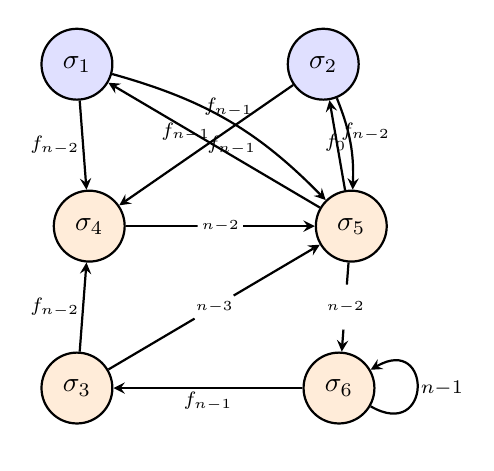
\begin{tikzpicture}[
  node distance=2.2cm,
  vtx/.style={circle, draw, thick, minimum size=9mm, inner sep=0pt},
  spine/.style={vtx, fill=blue!12},
  tooth/.style={vtx, fill=orange!15},
  arr/.style={-stealth, thick},
  lbl/.style={font=\scriptsize, inner sep=1pt},
  mlbl/.style={font=\scriptsize, inner sep=1pt, fill=white, circle},
]
  % Nodes
  \node[spine] (s1) {$\sigma_1$};
  \node[spine, right=2.2cm of s1] (s2) {$\sigma_2$};
  \node[tooth, below right=1.4cm and -0.5cm of s1] (s4) {$\sigma_4$};
  \node[tooth, right=2.4cm of s4] (s5) {$\sigma_5$};
  \node[tooth, below left=1.4cm and -0.5cm of s4] (s3) {$\sigma_3$};
  \node[tooth, right=2.4cm of s3] (s6) {$\sigma_6$};

  % Multiplicity-1 edges with map labels
  \draw[arr] (s5) -- node[lbl, above left]  {$f_{n-1}$} (s1);
  \draw[arr] (s5) -- node[lbl, above right] {$f_{n-2}$} (s2);
  \draw[arr] (s6) -- node[lbl, below]       {$f_{n-1}$} (s3);
  \draw[arr] (s1) -- node[lbl, left]        {$f_{n-2}$} (s4);
  \draw[arr] (s2) -- node[lbl, right=-1pt]  {$f_{n-1}$} (s4);
  \draw[arr] (s3) -- node[lbl, left]        {$f_{n-2}$} (s4);
  \draw[arr] (s1) to[bend left=15] node[lbl, above] {$f_{n-1}$} (s5);
  \draw[arr] (s2) to[bend left=12] node[lbl, left]  {$f_0$}     (s5);

  % Multiplicity >1 edges with count labels
  \draw[arr] (s3) -- node[mlbl] {{\tiny$n{-}3$}} (s5);
  \draw[arr] (s4) -- node[mlbl] {{\tiny$n{-}2$}} (s5);
  \draw[arr] (s5) -- node[mlbl] {{\tiny$n{-}2$}} (s6);
  \draw[arr] (s6) to[out=-30, in=30, looseness=5]
    node[lbl, right] {$n{-}1$} (s6);
\end{tikzpicture}
\caption{The boundary substitution graph of the comb IFS.  Vertices are
  the $6$~neighbor types: $\sigma_1, \sigma_2$ (spine--spine,
  sign~$+I$; shaded blue) and $\sigma_3, \ldots, \sigma_6$
  (spine--tooth or level-2, sign~$-I$; shaded orange).  A directed
  edge $\sigma_k \to \sigma_j$ means that the boundary piece~$B_k$
  contributes to~$B_j$ under substitution~\eqref{eq:bnd-rules}.
  Edges of multiplicity~$1$ are labelled with the producing map~$f_i$;
  edges of higher multiplicity show the count.
  The graph topology is independent of~$n$ (for $n \ge 3$); only the
  multiplicities depend on~$n$.}
\label{fig:neighbor-graph}
\end{figure}

% --------------------------------------------------------------------------
\subsection{Disk-Like Property}
\label{sec:disklike}

A self-similar tile $A$ is called \emph{disk-like} if it is homeomorphic to the
closed unit disk; see~\cite{bandt-wang,leung-lau} for criteria
and~\cite{akiyama-thuswaldner,ngai-tang} for surveys.  As noted in the Introduction, tiles with large
$\dH(\partial A)$ are generically non-disk-like, so achieving
$\dH(\partial A)$ close to~$2$ while maintaining the disk-like property
is particularly challenging.

The comb tiling is not a lattice tiling: the tooth map $f_{n-1}$ has
linear part~$-I$, so tiles related by~$f_{n-1}$ differ by a
$180^\circ$~rotation.  The tiling $\{A + d : d \in \Z^2\}$ must
therefore be replaced by a \emph{crystallographic tiling}
$\{\gamma(A) : \gamma \in \Gamma\}$, where $\Gamma$ is a discrete
cocompact group of isometries (a \emph{crystallographic group}).
For the comb family, $\Gamma$ is the ornament group~$p2$, generated by
two lattice translations and a $180^\circ$ rotation~$\rho$.
A compact set~$T$ satisfying a set equation of the form
$g(T) = \bigcup_{\delta \in D} \delta(T)$, where $g$ is an expanding
map and $D \subset \Gamma$ is a finite digit set, is called a
\emph{crystallographic reptile} (or \emph{crystile}) with respect
to~$\Gamma$~\cite[Definition~1]{loridant-luo-thuswaldner}.

For such a tiling, the \emph{neighbor set}
$S = \{\gamma \in \Gamma \setminus \{{\rm id}\} : T \cap \gamma(T)
\ne \emptyset\}$
and the \emph{boundary pieces}
$B_\gamma = T \cap \gamma(T)$ for $\gamma \in S$
are defined as before.  A neighbor $\gamma$ is an
\emph{edge neighbor} if $B_\gamma$ contains a point of the interior
of $T \cup \gamma(T)$; a neighbor is a \emph{vertex neighbor} if
$B_\gamma$ is a single point.  The set of edge neighbors is denoted
$\mathcal{A} \subseteq S$.

Two further graphs encode how boundary pieces meet after one
substitution step.  The \emph{double neighboring graph}~$G_2$ has
vertices $\{B_\gamma : \gamma \in S\}$, with an edge between
$B_{\gamma_1}$ and $B_{\gamma_2}$ whenever they intersect
($\gamma_1 \ne \gamma_2$).
For each $\gamma \in \mathcal{A}$, the \emph{boundary piece
graph}~$G_\gamma$ is the subgraph of~$G_2$ on the set of sub-pieces
\[
  V_\gamma \;=\;
  \bigl\{\, \delta\bigl(B_{\delta^{-1} g\gamma g^{-1}\delta'}\bigr)
  \;:\; \delta, \delta' \in D,\;
  \delta^{-1} g\gamma g^{-1}\delta' \in \mathcal{A} \,\bigr\};
\]
these are the images of boundary pieces that constitute
$g(B_\gamma)$ under the set
equation~\cite[Definition~4]{loridant-luo-thuswaldner}.
In our notation, with digits $f_i(x) = g^{-1}(\varepsilon_i x + d_i)$
and neighbors $\sigma_k = (\varepsilon_k, t_k)$, the vertices
of~$G_{\sigma_k}$ are exactly the sub-pieces $f_i(B_{\sigma_\ell})$
appearing on the right-hand side of the boundary substitution
rule~\eqref{eq:bnd-rules} for~$B_k$.

\begin{theorem}[{\cite[Theorem~4.2]{loridant-luo-thuswaldner}}]%
\label{thm:disklike-criterion}
Let $T \subset \R^2$ be a crystallographic reptile with respect
to~$\Gamma$, with expanding map~$g$ and digit set~$D$.
Let $S$ denote the set of neighbors and $\mathcal{A} \subseteq S$ the
subset of edge neighbors.  Then $T$~is disk-like if and only if:
\begin{enumerate}
\item[\rm(1)] for every pair of distinct $\gamma_1, \gamma_2 \in S$,
  the triple intersection
  $T \cap \gamma_1(T) \cap \gamma_2(T)$ is empty or a single point;
\item[\rm(2)] for each $\gamma \in \mathcal{A}$, the graph $G_\gamma$
  consists of a simple path;
\item[\rm(3)] the subgraph of~$G_2$ with
  vertices $\{B_\gamma : \gamma \in \mathcal{A}\}$ is a simple loop.
\end{enumerate}
\end{theorem}

We verify all three conditions for the comb family.

\begin{lemma}[Double neighboring graph --- condition~(3)]%
\label{lem:simple-loop}
For every $n \ge 3$, the double neighboring graph $G_2$ restricted to
the six edge neighbors $\sigma_1, \ldots, \sigma_6$ is the cycle
\[
  B_1 - B_3 - B_4 - B_2 - B_6 - B_5 - B_1.
\]
\end{lemma}

\begin{proof}
Two boundary pieces $B_j$ and $B_k$ ($j \ne k$) are connected by an
edge in $G_2$ if and only if $\sigma_j^{-1} \circ \sigma_k$ is a
neighbor, i.e., belongs to $\{\sigma_1, \ldots, \sigma_6\}$.

For $\sigma_j = (\varepsilon_j, t_j)$ and $\sigma_k = (\varepsilon_k, t_k)$,
the composition $\sigma_j^{-1} \circ \sigma_k$ has sign
$\varepsilon_j \varepsilon_k$ and translation
$\varepsilon_j(t_k - t_j)$.  We check all $\binom{6}{2} = 15$ pairs.
Writing $t_j$ for the translation vector of $\sigma_j$, the six
translations are:
\[
\begin{aligned}
  t_1 &= (n{-}1,\, 0), &\quad
  t_2 &= (-(n{-}1),\, 0), \\
  t_3 &= (3n{-}4,\, 2n{-}3), &\quad
  t_4 &= (2n{-}3,\, 2n{-}3), \\
  t_5 &= (2n{-}3,\, n{-}2), &\quad
  t_6 &= (n{-}2,\, n{-}2).
\end{aligned}
\]
The signs are $\varepsilon_1 = \varepsilon_2 = +I$,\;
$\varepsilon_3 = \varepsilon_4 = \varepsilon_5 = \varepsilon_6 = -I$.
Since $\varepsilon_j \varepsilon_k = +I$ when the signs are equal and
$-I$ when they differ, we compare $\varepsilon_j(t_k - t_j)$
with the known neighbor translations (and signs) to identify which
pairs are edges in~$G_2$.

The $6$~pairs that yield a neighbor $\sigma_\ell$ are:
\begin{alignat*}{3}
  &(1,3):&\quad &\sigma_1^{-1}\sigma_3 = (-I,\; t_3 - t_1) = \sigma_4,\\
  &(1,5):&\quad &\sigma_1^{-1}\sigma_5 = (-I,\; t_5 - t_1) = \sigma_6,\\
  &(2,4):&\quad &\sigma_2^{-1}\sigma_4 = (-I,\; t_4 - t_2) = \sigma_3,\\
  &(2,6):&\quad &\sigma_2^{-1}\sigma_6 = (-I,\; t_6 - t_2) = \sigma_5,\\
  &(3,4):&\quad &\sigma_3^{-1}\sigma_4 = (+I,\; -(t_4 - t_3)) = \sigma_1,\\
  &(5,6):&\quad &\sigma_5^{-1}\sigma_6 = (+I,\; -(t_6 - t_5)) = \sigma_1.
\end{alignat*}
The remaining $9$~pairs produce signed translations outside the six
neighbor translations:
\[
\begin{gathered}
  (1,2): (+I, (-(2n{-}2),0)),\quad
  (1,4): (-I, (n{-}2,2n{-}3)),\quad
  (1,6): (-I, (-1,n{-}2)),\\
  (2,3): (-I, (4n{-}5,2n{-}3)),\quad
  (2,5): (-I, (3n{-}4,n{-}2)),\\
  (3,5): (+I, (n{-}1,n{-}1)),\quad
  (3,6): (+I, (2n{-}2,n{-}1)),\\
  (4,5): (+I, (0,n{-}1)),\quad
  (4,6): (+I, (n{-}1,n{-}1)).
\end{gathered}
\]
None of these is equal to a signed translation of
$\sigma_1,\ldots,\sigma_6$ for $n \ge 3$.

The edges of $G_2$ are therefore $B_1 B_3$,\; $B_1 B_5$,\; $B_2 B_4$,\;
$B_2 B_6$,\; $B_3 B_4$,\; $B_5 B_6$.\;  Each vertex has degree~$2$,
and the graph is the $6$-cycle
$B_1 - B_3 - B_4 - B_2 - B_6 - B_5 - B_1$.
\end{proof}

\begin{figure}[ht]
\centering
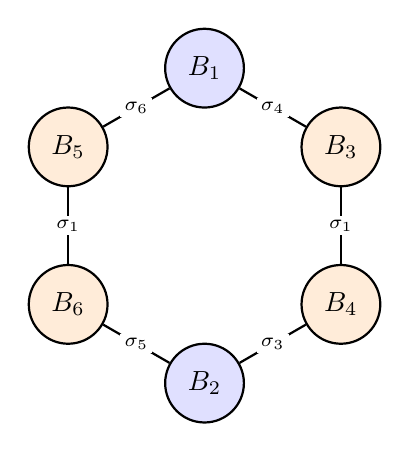
\begin{tikzpicture}[
  bvtx/.style={circle, draw, thick, minimum size=10mm, inner sep=0pt},
  bspine/.style={bvtx, fill=blue!12},
  btooth/.style={bvtx, fill=orange!15},
  elbl/.style={font=\scriptsize, fill=white, inner sep=1.5pt},
]
  % Vertices on a regular hexagon (clockwise: B1, B3, B4, B2, B6, B5)
  \node[bspine] (B1) at ( 90:2cm) {$B_1$};
  \node[btooth] (B3) at ( 30:2cm) {$B_3$};
  \node[btooth] (B4) at (330:2cm) {$B_4$};
  \node[bspine] (B2) at (270:2cm) {$B_2$};
  \node[btooth] (B6) at (210:2cm) {$B_6$};
  \node[btooth] (B5) at (150:2cm) {$B_5$};

  % Edges with mediating-neighbor labels
  \draw[thick] (B1) -- node[elbl]         {$\sigma_4$} (B3);
  \draw[thick] (B3) -- node[elbl]         {$\sigma_1$} (B4);
  \draw[thick] (B4) -- node[elbl]         {$\sigma_3$} (B2);
  \draw[thick] (B2) -- node[elbl]         {$\sigma_5$} (B6);
  \draw[thick] (B6) -- node[elbl]         {$\sigma_1$} (B5);
  \draw[thick] (B5) -- node[elbl]         {$\sigma_6$} (B1);
\end{tikzpicture}
\caption{The double neighboring graph~$G_2$ for the comb family
  (Lemma~\ref{lem:simple-loop}).  The six boundary pieces form a
  hexagonal cycle.  Edge labels indicate the mediating neighbor:
  $B_j$--$B_k$ is an edge when
  $\sigma_j^{-1}\sigma_k = \sigma_\ell \in \mathcal{A}$.
  Spine-type pieces $B_1, B_2$ are shaded blue; tooth-type pieces
  $B_3, \ldots, B_6$ orange.  Note that $\sigma_1$ appears on two
  opposite edges ($B_3 B_4$ and $B_5 B_6$): it is the cross-map
  link that connects consecutive spine maps in the
  graphs~$G_{\sigma_5}$ and~$G_{\sigma_6}$.}
\label{fig:g2-cycle}
\end{figure}

\begin{lemma}[Boundary piece graphs --- condition~(2)]%
\label{lem:simple-path}
For every $n \ge 3$ and every edge neighbor $\gamma \in \{\sigma_1,
\ldots, \sigma_6\}$, the graph $G_\gamma$ is a simple path.
\end{lemma}

\begin{proof}
The graph $G_\gamma$ has one vertex for each sub-piece appearing
in the boundary substitution rule~\eqref{eq:bnd-rules} for~$B_\gamma$,
and an edge between two sub-pieces when they are pairwise neighbors at
the next refinement level.  We verify the path structure for each
boundary piece.

\emph{Case $B_1$, $B_2$, $B_3$.}
The rules $B_1 = f_{n-1}(B_5)$,\; $B_2 = f_{n-2}(B_5)$,\;
$B_3 = f_{n-1}(B_6)$ each contain a single sub-piece.  A graph on one
vertex is a (trivial) simple path.

\emph{Case $B_4$.}
The rule is $B_4 = f_{n-2}(B_1) \cup f_{n-2}(B_3) \cup f_{n-1}(B_2)$.
We check adjacency of the three sub-pieces.  Two sub-pieces
$f_i(B_j)$ and $f_k(B_\ell)$ are neighbors if $f_i^{-1}\sigma_4 f_k$
composed with the neighbor data of $B_j, B_\ell$ yields a neighbor.
Since $f_{n-2}$ and $f_{n-1}$ are adjacent maps (their level-1
neighbor is $\sigma_4$), and both $B_1$ and $B_3$ touch $B_2$
in the cyclic order of~$G_2$ (Lemma~\ref{lem:simple-loop}), the
three sub-pieces form a path:
$f_{n-2}(B_1) - f_{n-2}(B_3) - f_{n-1}(B_2)$.

\emph{Case $B_5$.}
The rule~\eqref{eq:bnd-rules} gives $2n{-}3$ sub-pieces.  For $n \ge 4$
these are
\[
  f_0(B_2),\; f_0(B_4),\; f_0(B_3),\;
  f_1(B_4),\; f_1(B_3),\; \ldots,\;
  f_{n-4}(B_4),\; f_{n-4}(B_3),\;
  f_{n-3}(B_4),\; f_{n-1}(B_1);
\]
for $n = 3$ the $B_3$-union in~\eqref{eq:bnd-rules} is empty and the
three sub-pieces are $f_0(B_2),\, f_0(B_4),\, f_2(B_1)$.
Two sub-pieces from the \emph{same} map~$f_j$ are adjacent in~$G_{\sigma_5}$
when the corresponding boundary pieces are adjacent in~$G_2$.
Since $B_2 B_4$ and $B_3 B_4$ are edges of~$G_2$
(Lemma~\ref{lem:simple-loop}) but $B_2 B_3$ is not,
the three sub-pieces from~$f_0$ form the path
$f_0(B_2) - f_0(B_4) - f_0(B_3)$.

For \emph{cross-map} adjacency between $f_j$ and $f_{j+1}$
($j, j{+}1 \le n{-}2$), the level-1 neighbor map is
$\sigma_1 = f_j^{-1} f_{j+1}$.
A sub-piece $f_j(B_\alpha)$ intersects $f_{j+1}(B_\beta)$ only
if $B_\alpha$ meets~$B_1$ and $B_\beta$ meets~$B_2$ in~$G_2$.
Among the indices appearing in the rule for $B_5$, namely
$\{B_1, B_2, B_3, B_4\}$, only $B_3$ is adjacent to~$B_1$ and
only $B_4$ is adjacent to~$B_2$, so the unique cross-map edge is
$f_j(B_3) - f_{j+1}(B_4)$.

The last transition from $f_{n-3}(B_4)$ to $f_{n-1}(B_1)$ uses
$\sigma_3 = f_{n-3}^{-1}f_{n-1}$: we need $B_4$ adjacent to~$B_3$
and $B_1$ adjacent to~$B_3$ in~$G_2$, both of which hold.

No non-consecutive sub-pieces are adjacent: maps $f_j, f_\ell$ with
$|j - \ell| \ge 2$ have tiles of $x_1$-diameter at most $2n{-}3$
separated by distance $(n{-}1)|j - \ell| - (2n{-}3) > 0$.
Hence the path is (for $n \ge 4$):
\begin{align*}
  &f_0(B_2) - f_0(B_4) - f_0(B_3) - f_1(B_4) - f_1(B_3) - \cdots\\
  &\quad\cdots - f_{n-4}(B_3) - f_{n-3}(B_4) - f_{n-1}(B_1),
\end{align*}
while for $n = 3$ it degenerates to
$f_0(B_2) - f_0(B_4) - f_2(B_1)$, with the last edge via
$\sigma_3 = f_0^{-1} f_2$.
In all cases $G_{\sigma_5}$ is a simple path on $2n{-}3$ vertices.

\emph{Case $B_6$.}
The rule gives $2n{-}3$ sub-pieces:
\[
  f_0(B_6),\; f_0(B_5),\; f_1(B_6),\; f_1(B_5),\;
  \ldots,\; f_{n-3}(B_6),\; f_{n-3}(B_5),\; f_{n-2}(B_6).
\]
Within each~$f_j$, the sub-pieces $f_j(B_5)$ and $f_j(B_6)$ are
adjacent ($B_5 B_6$ is an edge of~$G_2$).
For the cross-map adjacency via $\sigma_1 = f_j^{-1}f_{j+1}$:
among the indices appearing in the rule for $B_6$, namely
$\{B_5, B_6\}$, only $B_5$ is adjacent to~$B_1$ and only
$B_6$ is adjacent to~$B_2$ in~$G_2$, so the unique cross-map edge
is $f_j(B_5) - f_{j+1}(B_6)$.
No non-consecutive sub-pieces are neighbors (same separation argument).
Hence $G_{\sigma_6}$ is the simple path
\[
  f_0(B_6) - f_0(B_5) - f_1(B_6) - f_1(B_5) - \cdots
  - f_{n-3}(B_5) - f_{n-2}(B_6).
  \qedhere
\]
\end{proof}

\begin{figure}[ht]
\centering
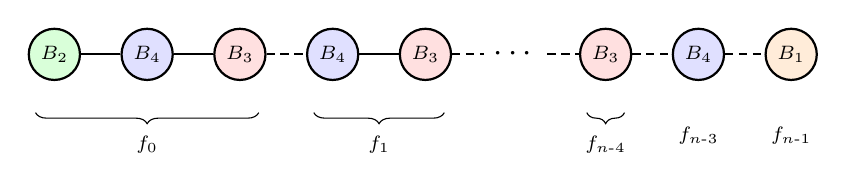
\begin{tikzpicture}[
  pnode/.style={circle, draw, thick, minimum size=6.5mm, inner sep=0pt,
                font=\scriptsize},
  p2/.style={pnode, fill=green!15},
  p4/.style={pnode, fill=blue!12},
  p3/.style={pnode, fill=red!12},
  p1/.style={pnode, fill=orange!15},
  intra/.style={thick},
  cross/.style={thick, densely dashed},
  maplbl/.style={font=\scriptsize, below=3pt},
]
  % Row of nodes for the G_{sigma_5} path (general n)
  \node[p2]                  (v1) {$B_2$};
  \node[p4, right=5mm of v1] (v2) {$B_4$};
  \node[p3, right=5mm of v2] (v3) {$B_3$};
  \node[p4, right=5mm of v3] (v4) {$B_4$};
  \node[p3, right=5mm of v4] (v5) {$B_3$};
  \node[right=4mm of v5, font=\large] (dots) {$\cdots$};
  \node[p3, right=4mm of dots] (v6) {$B_3$};
  \node[p4, right=5mm of v6] (v7) {$B_4$};
  \node[p1, right=5mm of v7] (v8) {$B_1$};

  % Intra-map edges (solid)
  \draw[intra] (v1) -- (v2);
  \draw[intra] (v2) -- (v3);
  \draw[intra] (v4) -- (v5);

  % Cross-map edges (dashed)
  \draw[cross] (v3) -- (v4);
  \draw[cross] (v5) -- (dots);
  \draw[cross] (dots) -- (v6);
  \draw[cross] (v6) -- (v7);
  \draw[cross] (v7) -- (v8);

  % Map-index braces
  \draw[decorate, decoration={brace, mirror, amplitude=4pt}]
    ([yshift=-5mm]v1.south west) -- ([yshift=-5mm]v3.south east)
    node[midway, below=5pt, font=\scriptsize] {$f_0$};
  \draw[decorate, decoration={brace, mirror, amplitude=4pt}]
    ([yshift=-5mm]v4.south west) -- ([yshift=-5mm]v5.south east)
    node[midway, below=5pt, font=\scriptsize] {$f_1$};
  \draw[decorate, decoration={brace, mirror, amplitude=4pt}]
    ([yshift=-5mm]v6.south west) -- ([yshift=-5mm]v6.south east)
    node[midway, below=5pt, font=\scriptsize] {$f_{n\text{-}4}$};
  \node[font=\scriptsize, below=8mm] at (v7) {$f_{n\text{-}3}$};
  \node[font=\scriptsize, below=8mm] at (v8) {$f_{n\text{-}1}$};
\end{tikzpicture}
\caption{The boundary piece graph $G_{\sigma_5}$ for the
  comb family (Lemma~\ref{lem:simple-path}, Case~$B_5$).
  Solid edges connect sub-pieces within the same
  map~$f_j$ (adjacency in~$G_2$); dashed edges connect
  sub-pieces from consecutive maps $f_j, f_{j+1}$ via the
  cross-map neighbor~$\sigma_1$.  Each cross-map link is uniquely
  determined: $B_3$ is the only sub-piece adjacent to~$B_1$, and
  $B_4$ the only one adjacent to~$B_2$ in~$G_2$
  (Figure~\ref{fig:g2-cycle}), so the edge must be
  $f_j(B_3)$--$f_{j+1}(B_4)$.  The graph is a simple path on
  $2n{-}3$ vertices.}
\label{fig:g-sigma5}
\end{figure}

\begin{theorem}[Disk-like]\label{thm:disklike}
For every integer $n \ge 2$, the comb tile $C_n$ is disk-like.
\end{theorem}

\begin{proof}
For $n = 2$, the attractor $C_2$ is a rectangle, so the claim is
trivial.  For $n \ge 3$, conditions~(2) and~(3) of
Theorem~\ref{thm:disklike-criterion} are established in
Lemmas~\ref{lem:simple-path} and~\ref{lem:simple-loop}; it remains to
verify condition~(1).  We identify the first-level intersection graph,
show it has a unique triangle, and prove the corresponding triple
intersection is a single point.

\emph{Step~1: First-level intersection graph.}
Two first-level tiles $f_i(C)$ and $f_j(C)$ intersect if and only if
$f_i^{-1} \circ f_j$ is a neighbor.
By Proposition~\ref{prop:level1}, the only level-1 neighbor maps are
$\sigma_1, \ldots, \sigma_4$.  These correspond to the pairs:
\begin{itemize}
\item Spine consecutive: $(j,\, j{+}1)$ for $j = 0, \ldots, n{-}3$,
  giving $\sigma_1$ (or its inverse $\sigma_2$);
\item Tooth: $(n{-}3,\, n{-}1)$ giving $\sigma_3$, and
  $(n{-}2,\, n{-}1)$ giving $\sigma_4$.
\end{itemize}
The resulting graph is a path $0 {-} 1 {-} \cdots {-} (n{-}2)$ with
vertex~$n{-}1$ adjacent to $n{-}3$ and~$n{-}2$.  Its only clique of
size~$3$ is $\{n{-}3,\; n{-}2,\; n{-}1\}$.

\emph{Step~2: Triple refinement is unique.}
Write $T = f_{n-3}(C) \cap f_{n-2}(C) \cap f_{n-1}(C)$ for the
unique triple intersection.  Substituting $C = \bigcup_k f_k(C)$,
\[
  T = \bigcup_{\substack{a,b,c \\ \text{pairwise}\\\text{feasible}}}
  f_{n-3} \circ f_a(C) \;\cap\;
  f_{n-2} \circ f_b(C) \;\cap\;
  f_{n-1} \circ f_c(C),
\]
where a triple $(a, b, c)$ is \emph{pairwise feasible} if
$f_a^{-1} \sigma_1 f_b$,\; $f_b^{-1} \sigma_4 f_c$,\;
$f_a^{-1} \sigma_3 f_c$ are all neighbors.
Here $\sigma_1 = f_{n-3}^{-1} f_{n-2}$,
$\sigma_4 = f_{n-2}^{-1} f_{n-1}$,
$\sigma_3 = f_{n-3}^{-1} f_{n-1}$ are the three pairwise neighbor
maps of the triangle.

The key observation: $\sigma_1$ and $\sigma_2$ each have exactly
\emph{one} surviving child under refinement~\eqref{eq:child}.
For~$\sigma_1 = (+I, (n{-}1, 0))$, the vector $gt = g \cdot (n{-}1, 0) =
(0,\, n{-}1)$.  All spine--spine children
$f_\alpha^{-1} \sigma_1 f_\beta$ (with $\alpha, \beta \le n{-}2$)
have translation component
$t_2' = n{-}1 > n{-}1{-}1/n = \mathrm{height}(R)$,
so they exceed the $R$-bound
and are infeasible.  We check the three remaining child types
(those involving the tooth index $n{-}1$):
\begin{itemize}
\item \emph{Spine--tooth} ($\alpha \le n{-}2$, $j = n{-}1$):
  sign~$-I$, translation $\bigl((n{-}1)(n{-}\alpha)-1,\; 3n{-}4\bigr)$.
  The $x_2$-component $3n{-}4$ exceeds the sum
  $2 \cdot \mathrm{height}(R) = 2(n{-}1{-}1/n)$ for $n \ge 3$,
  so $C \cap \sigma(C) = \emptyset$ for all~$\alpha$.
\item \emph{Tooth--tooth} ($\alpha = j = n{-}1$):
  sign~$+I$, translation $(0,\,{-}(n{-}1))$.
  This requires $x_2 \ge n{-}1$ in~$C$, but
  $C \subset R$ has $x_2 \le n{-}1{-}1/n$; infeasible.
\item \emph{Tooth--spine} ($\alpha = n{-}1$, $\beta \le n{-}2$):
  sign~$-I$, translation $\bigl((n{-}1)(n{-}\beta)-1,\; n{-}2\bigr)$.
  For $\beta \le n{-}3$ the first component
  $(n{-}1)(n{-}\beta)-1 \ge 3n{-}4$, forcing both summands in the
  $C + C$ representation into the tooth strip
  ($x_1 \ge n{-}1$, hence $x_2 \ge (n{-}1)(n{-}2)/n$
  by Lemma~\ref{lem:tooth-strip}); then
  $p_2 + q_2 \ge 2(n{-}1)(n{-}2)/n > n{-}2$ for $n \ge 3$,
  contradicting $p_2 + q_2 = n{-}2$.
  Only $\beta = n{-}2$ survives, giving translation $(2n{-}3,\,n{-}2)$.
\end{itemize}
Thus the unique surviving child is
\[
  f_{n-1}^{-1} \circ \sigma_1 \circ f_{n-2} = \sigma_5,
\]
which fixes $a = n{-}1$ and $b = n{-}2$.

With $a = n{-}1$ fixed, we evaluate the children of~$\sigma_3$
at $(n{-}1,\, c)$.  For spine indices $c \le n{-}2$, the
translation has $|t_2'| = n{-}1 > \mathrm{height}(R)$ (infeasible),
while for $c = n{-}1$ the child is
\[
  f_{n-1}^{-1} \circ \sigma_3 \circ f_{n-1} = \sigma_6.
\]
This forces $c = n{-}1$.  A consistency check confirms
$f_{n-2}^{-1} \circ \sigma_4 \circ f_{n-1} = \sigma_1$.
Thus the unique refinement triple is $(a, b, c) = (n{-}1, n{-}2,
n{-}1)$, and the new pairwise state is $(\sigma_5,\, \sigma_1,\,
\sigma_6)$.

\emph{Step~3: Period-$2$ cycle.}
Iterating the same analysis for the state
$(\sigma_5,\, \sigma_1,\, \sigma_6)$:
\begin{itemize}
\item $\sigma_1$ (the ``bottleneck'') again forces $b = n{-}1$,
  $c = n{-}2$, giving $\sigma_5$.
\item For $\sigma_5$, the child $f_\alpha^{-1} \sigma_5 f_{n-1}$
  with spine~$\alpha$ has translation
  $t_1' = -(n{-}1)(1{+}\alpha)$.  Only $\alpha = 0$ yields
  $|t_1'| = n{-}1 \le 2n{-}3$, giving $\sigma_2$.  So $a = 0$.
\item $f_0^{-1} \circ \sigma_6 \circ f_{n-2} = \sigma_6$ (since
  $0 + (n{-}2) = n{-}2$).
\end{itemize}
The new state is $(\sigma_2,\, \sigma_5,\, \sigma_6)$.

One more iteration is explicit.  The mirror bottleneck $\sigma_2$
forces $(a,b)=(n{-}2,n{-}1)$ and gives the child $\sigma_5$.
With $b=n{-}1$, the only child of $\sigma_5$ that remains feasible
is the tooth--spine child with $c=0$, which is $\sigma_1$ by
Step~4.  Finally $f_{n-2}^{-1}\sigma_6 f_0=\sigma_6$ since
$(n{-}2)+0=n{-}2$.  Thus the state returns to
$(\sigma_5,\, \sigma_1,\, \sigma_6)$.

The refinement thus cycles with period~$2$:
\[
  (\sigma_5, \sigma_1, \sigma_6)
  \;\longrightarrow\;
  (\sigma_2, \sigma_5, \sigma_6)
  \;\longrightarrow\;
  (\sigma_5, \sigma_1, \sigma_6)
  \;\longrightarrow\; \cdots
\]
At each level, the triple intersection is covered by a single
level-$k$ tile of diameter $O(n^{-k/2})$.  As $k \to \infty$,
the nested compact sets converge to a single point.

It remains to translate this first-level triple calculation into
condition~\textup{(1)} of Theorem~\ref{thm:disklike-criterion}.
For any two distinct neighbors $\sigma_j,\sigma_k$, the triple
intersection
\[
  C \cap \sigma_j(C) \cap \sigma_k(C)
\]
is exactly $B_j \cap B_k$.  Hence it is empty unless $B_jB_k$ is an
edge of the double neighboring graph~$G_2$.  By
Lemma~\ref{lem:simple-loop}, the only non-empty cases are the six
cycle edges
\[
  B_1B_3,\quad B_3B_4,\quad B_4B_2,\quad
  B_2B_6,\quad B_6B_5,\quad B_5B_1.
\]
The initial first-level triple
$f_{n-3}(C)\cap f_{n-2}(C)\cap f_{n-1}(C)$ accounts for the first
three of these after applying respectively
$f_{n-3}^{-1}$, $f_{n-1}^{-1}$, and $f_{n-2}^{-1}$:
\[
  B_1\cap B_3,\qquad B_3\cap B_4,\qquad B_2\cap B_4 .
\]
The unique first refinement of that triple has pairwise state
$(\sigma_5,\sigma_1,\sigma_6)$, and applying the inverse of its
first, third, and second level-$2$ pieces gives respectively
\[
  B_5\cap B_6,\qquad B_2\cap B_6,\qquad B_1\cap B_5 .
\]
Both triple states are contained in the nested singleton constructed
above, so each of the six non-empty intersections $B_j\cap B_k$ is a
single point.  This verifies condition~\textup{(1)}.

Condition~(2) holds by
Lemma~\ref{lem:simple-path}, and condition~(3) by
Lemma~\ref{lem:simple-loop}.  Hence $C_n$ is disk-like for all
$n \ge 3$ (and hence for all $n \ge 2$).
\end{proof}

\begin{figure}[ht]
\centering
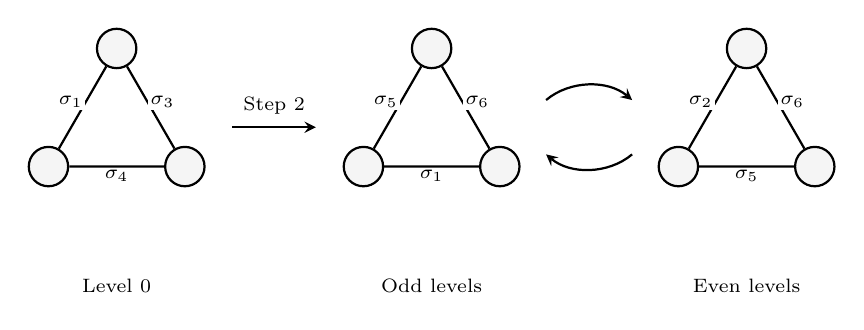
\begin{tikzpicture}[
  tv/.style={circle, draw, thick, minimum size=5mm, inner sep=0pt,
             font=\scriptsize, fill=gray!8},
  tlbl/.style={font=\scriptsize, fill=white, inner sep=1pt},
  trans/.style={-stealth, thick, shorten >=2pt, shorten <=2pt},
  cyc/.style={-stealth, thick, shorten >=2pt, shorten <=2pt,
              bend left=40},
  steplbl/.style={font=\scriptsize, above=1pt},
]
  % --- Triangle 0 (initial) ---
  \begin{scope}[shift={(0,0)}]
    \node[tv] (a0) at (90:1cm)  {};
    \node[tv] (b0) at (210:1cm) {};
    \node[tv] (c0) at (330:1cm) {};
    \draw[thick] (a0) -- node[tlbl, above right=-2pt] {$\sigma_3$} (c0)
                 -- node[tlbl, below]                  {$\sigma_4$} (b0)
                 -- node[tlbl, above left=-2pt]        {$\sigma_1$} (a0);
    \node[font=\scriptsize, below=13mm] at (0,-0.5) {Level $0$};
  \end{scope}

  % Arrow
  \draw[trans] (1.4,0) -- node[steplbl] {Step 2} (2.6,0);

  % --- Triangle 1 ---
  \begin{scope}[shift={(4,0)}]
    \node[tv] (a1) at (90:1cm)  {};
    \node[tv] (b1) at (210:1cm) {};
    \node[tv] (c1) at (330:1cm) {};
    \draw[thick] (a1) -- node[tlbl, above right=-2pt] {$\sigma_6$} (c1)
                 -- node[tlbl, below]                  {$\sigma_1$} (b1)
                 -- node[tlbl, above left=-2pt]        {$\sigma_5$} (a1);
    \node[font=\scriptsize, below=13mm] at (0,-0.5) {Odd levels};
  \end{scope}

  % Arrows for the period-2 cycle
  \draw[cyc] (5.4, 0.3) to node[steplbl, above=2pt] {} (6.6, 0.3);
  \draw[cyc] (6.6,-0.3) to node[steplbl, below=2pt] {} (5.4,-0.3);

  % --- Triangle 2 ---
  \begin{scope}[shift={(8,0)}]
    \node[tv] (a2) at (90:1cm)  {};
    \node[tv] (b2) at (210:1cm) {};
    \node[tv] (c2) at (330:1cm) {};
    \draw[thick] (a2) -- node[tlbl, above right=-2pt] {$\sigma_6$} (c2)
                 -- node[tlbl, below]                  {$\sigma_5$} (b2)
                 -- node[tlbl, above left=-2pt]        {$\sigma_2$} (a2);
    \node[font=\scriptsize, below=13mm] at (0,-0.5) {Even levels};
  \end{scope}
\end{tikzpicture}
\caption{Triple-point refinement (Theorem~\ref{thm:disklike},
  condition~(1)).  Each triangle shows the pairwise neighbor
  state of the three tiles meeting at the triple point.
  After one refinement (Step~2), the state enters a period-$2$
  cycle: the pair $\{\sigma_5, \sigma_6\}$ persists while the
  third edge alternates between $\sigma_1$ and~$\sigma_2$.
  Since each level nests inside a single tile of diameter
  $O(n^{-k/2})$, the triple intersection converges to a point.}
\label{fig:triple-refinement}
\end{figure}

\begin{remark}
Both the neighbor graph (Theorem~\ref{thm:graph}) and the disk-like
property (Theorem~\ref{thm:disklike}) are proved for all $n \ge 3$ by
the same structural argument: the combinatorial pattern of neighbors
and their children depends only on the relative positions of the
spine endpoint, the tooth, and their immediate predecessors,
not on the spine length.  Only the translations change with~$n$.
\end{remark}

\begin{remark}[Topological structure of $C_n$]
\label{rem:topology}
The disk-like property, together with the explicit structure of~$G_2$
and the boundary substitution~\eqref{eq:bnd-rules}, yields a
complete topological description of the comb tiling.

\begin{enumerate}
\item \emph{Jordan boundary.}
Since $C_n$ is disk-like, $C_n \cong \overline{\mathbb{D}}$ and
$\partial C_n$ is a Jordan curve (by the Sch\"onflies theorem).

\item \emph{Six boundary arcs in cyclic order.}
The $G_2$-cycle
$B_1 \!-\! B_3 \!-\! B_4 \!-\! B_2 \!-\! B_6 \!-\! B_5 \!-\! B_1$
(Lemma~\ref{lem:simple-loop}) determines a decomposition of
$\partial C_n$ into six arcs, each of which is the common boundary
with one neighbor.  Adjacent arcs in the cycle meet at exactly one
point.

\item \emph{Six triple points.}
The six arc junctions are the only points where three or more tiles
meet (condition~(1) of Theorem~\ref{thm:disklike-criterion}).
Each such point has valence~$3$ in the tiling.

\item \emph{Hexagonal combinatorial type.}
Although $\dH(\partial C_n) \to 2$ as $n \to \infty$
(Theorem~\ref{thm:dim}), the combinatorics of the tiling is
independent of~$n$ and coincides with that of the regular hexagonal
tiling: every tile has exactly $6$ edge neighbors and $6$ vertices,
with vertex valence~$3$.

\item \emph{Self-similar arc structure.}
The substitution rules~\eqref{eq:bnd-rules} and the simple-path
property of the graphs $G_{\sigma_k}$
(Lemma~\ref{lem:simple-path}) imply that each boundary arc is an
IFS attractor in its own right: at every substitution step the
sub-pieces of each arc form a chain without branching or loops,
so the arc remains a topological arc at every scale.
\end{enumerate}
\end{remark}

% --------------------------------------------------------------------------
\subsection{Boundary Dimension}
\label{sec:dim}

\subsubsection{Derivation of the quartic}

\begin{theorem}[Boundary dimension formula]\label{thm:dim}
For every integer $n \ge 3$, the characteristic polynomial of $M_n$
factors as
\begin{equation}\label{eq:charpoly-factor}
  \det(\lambda I - M_n) = \lambda^2 \cdot p_n(\lambda),
\end{equation}
where $p_n$ is the quartic polynomial
\begin{equation}\label{eq:quartic}
  p_n(x) = x^4 - (n{-}1)\,x^3 - 2\,x^2 - (n{-}1)(n{-}4)\,x + n(n{-}2).
\end{equation}
The spectral radius $\lambda_n = \rho(M_n)$ is the unique root of $p_n$
in the interval $(n{-}1,\, n)$, and the boundary Hausdorff dimension is
\begin{equation}\label{eq:dim}
  \dH(\partial C_n) = \frac{2\log\lambda_n}{\log n}.
\end{equation}
\end{theorem}

\begin{proof}
The dimension formula~\eqref{eq:dim} follows from the
Mauldin--Williams theory~\cite{mauldin-williams} applied to the
boundary GIFS~\eqref{eq:bnd-rules}.  Since the original IFS
satisfies the OSC with $V = \operatorname{int}(A)$
(Theorem~\ref{thm:graph}), the boundary GIFS inherits the
hypotheses of~\cite{mauldin-williams};
see also~\cite{duvall-keesling-strichartz} for the same approach
applied to the boundaries of self-similar tiles.  All contractions
share the ratio $r = 1/\sqrt{n}$, so
$\dH(\partial C_n) = 2\log\rho(M_n)/\log n$.

To prove the factorisation~\eqref{eq:charpoly-factor}, we solve the
eigenvector equation $M_n v = \lambda v$ for $\lambda \ne 0$.
From the first three rows:
\[
  B_1 = B_2 = \frac{B_5}{\lambda}, \qquad
  B_3 = \frac{B_6}{\lambda}.
\]
Substituting into row~6:
$\lambda B_6 = (n{-}2) B_5 + (n{-}1) B_6$, whence
\begin{equation}\label{eq:B6-from-B5}
  B_6 = \frac{(n{-}2)\, B_5}{\lambda - (n{-}1)}.
\end{equation}
Substituting all of $B_1, B_2, B_3, B_6$ in terms of $B_5$ into row~4:
\[
  \lambda B_4 = \frac{2}{\lambda}\, B_5
    + \frac{(n{-}2)}{\lambda\bigl(\lambda-(n{-}1)\bigr)}\, B_5
  = \frac{B_5}{\lambda}\,\cdot\, \frac{2\lambda - n}{\lambda - (n{-}1)},
\]
giving
\begin{equation}\label{eq:B4-from-B5}
  B_4 = \frac{(2\lambda - n)\, B_5}
    {\lambda^2\bigl(\lambda - (n{-}1)\bigr)}.
\end{equation}
Finally, substituting into row~5:
\begin{align*}
  \lambda B_5 &= \frac{2}{\lambda}\, B_5
    + \frac{(n{-}3)(n{-}2)}{\lambda\bigl(\lambda-(n{-}1)\bigr)}\, B_5
    + \frac{(n{-}2)(2\lambda-n)}
      {\lambda^2\bigl(\lambda-(n{-}1)\bigr)}\, B_5.
\end{align*}
Dividing by $B_5 \ne 0$ and multiplying through by
$\lambda^2(\lambda-(n{-}1))$:
\begin{align*}
  \lambda^3\bigl(\lambda-(n{-}1)\bigr)
  &= 2\lambda\bigl(\lambda-(n{-}1)\bigr) \\
  &\quad + (n{-}3)(n{-}2)\lambda + (n{-}2)(2\lambda-n).
\end{align*}
Expanding and collecting terms, the right-hand side equals
$2\lambda^2 + (n{-}1)(n{-}4)\lambda - n(n{-}2)$, so we obtain
\[
  \lambda^4 - (n{-}1)\lambda^3 - 2\lambda^2
    - (n{-}1)(n{-}4)\lambda + n(n{-}2) = 0,
\]
which is $p_n(\lambda) = 0$.

The factor $\lambda^2$ accounts for the two zero eigenvalues arising from
the two linear dependencies in~$M_n$: the identical rows for $B_1$
and~$B_2$, and the relation
$(n{-}2) \cdot (\text{row } B_1) + (n{-}1) \cdot (\text{row } B_3)
 = \text{row } B_6$.
\end{proof}

\begin{remark}[Relation to the general decomposition of Subsection~\ref{sec:asymp}]
\label{rem:quartic-link}
The six neighbor indices $B_1, \ldots, B_6$ of $M_n^{(2)}$ are the
$d = 2$ instance of the Bandt set
$\mathcal{N}(2, n) = \mathcal{B}_+(2, n) \sqcup \mathcal{B}_-(2, n)$,
reproducing $p(2) = H_3 - 1 = 6$ of
Corollary~\ref{cor:pell}.  Comparing the row of
$M_n^{(2)}$ for $B_4$ and $B_6$ with the sub-case description of
Subsubsection~\ref{sec:Mn-decomp} identifies $A^{(2)}$ (the rows with
linear-in-$n$ entries, from sub-cases A1 and B1) and $B^{(2)}$
(the residual integer matrix).  The two zero eigenvalues in
\eqref{eq:charpoly-factor} are the $d = 2$ instance of the
general nullity formula $\dim\ker M_n^{(d)} = 2 P_{d-1}$
\textup{(}$2 P_1 = 2$\textup{)}; see
Theorem~\ref{thm:nullity-equal}.
\end{remark}

\begin{remark}[Root location]
The polynomial $p_n$ satisfies:
\begin{alignat*}{2}
  p_n(n{-}1) &= -(n{-}2)(n^2{-}3n{+}1) &&< 0 \quad (n \ge 3), \\
  p_n(n)     &= 2n(2n{-}3)              &&> 0 \quad (n \ge 3),
\end{alignat*}
so the intermediate value theorem guarantees a root in $(n{-}1,\,n)$.
Uniqueness follows from Descartes' rule: the coefficients of $p_n$ exhibit
exactly two sign changes for $n \ge 3$, so $p_n$ has at most two positive
real roots; since a second root $\mu_n \in (1,n{-}1)$ is accounted for
separately (see Subsection~\ref{ssec:roots}), the root in $(n{-}1,n)$ is unique.
Since $p_n(0) = n(n{-}2) > 0$ for $n \ge 3$ and $p_n(1) = 2(n{-}2) > 0$,
there is also a root between $1$ and $n{-}1$; the dominant root is the
one in $(n{-}1,\,n)$.
\end{remark}

\subsubsection{Computed dimensions}

Table~\ref{tab:dims} lists the boundary dimension for selected values
of~$n$.

\begin{table}[h]
\centering
\caption{Boundary dimension of the comb tile $C_n$ for selected $n$.
The polynomial is $p_n(x)$ from~\eqref{eq:quartic}.}
\label{tab:dims}
\begin{tabular}{rccc}
\toprule
$n$ & $\lambda_n$ & $\dH(\partial C_n)$ & $2 - \dH(\partial C_n)$ \\
\midrule
  3 & 2.2213 & 1.4529 & 0.5471 \\
  4 & 3.3846 & 1.7590 & 0.2410 \\
  5 & 4.4790 & 1.8633 & 0.1367 \\
  6 & 5.5451 & 1.9120 & 0.0880 \\
  7 & 6.5951 & 1.9388 & 0.0612 \\
  8 & 7.6345 & 1.9550 & 0.0450 \\
  9 & 8.6665 & 1.9656 & 0.0344 \\
 10 & 9.6932 & 1.9729 & 0.0271 \\
 20 & 19.8279 & 1.9942 & 0.0058 \\
 50 & 49.9251 & 1.9992 & $7.67 \times 10^{-4}$ \\
100 & 99.9613 & 1.9998 & $1.68 \times 10^{-4}$ \\
\bottomrule
\end{tabular}
\end{table}

All numerical values in Tables~\ref{tab:dims} and~\ref{tab:ratio}
are computed from the dominant real root~$\lambda_n$ of the
explicit quartic~\eqref{eq:quartic} via the
formula~\eqref{eq:dim}; no numerical simulation of the IFS is
involved.

\subsubsection{Asymptotic expansion of the dominant root}

\begin{theorem}[Asymptotics]\label{thm:asymp}
The dominant root $\lambda_n$ of $p_n(x)$ satisfies
\begin{equation}\label{eq:lambda-asymp}
  \lambda_n = n - \frac{4}{n} + O\!\left(\frac{1}{n^2}\right)
  \qquad (n \to \infty).
\end{equation}
Consequently,
\begin{equation}\label{eq:dim-asymp}
  2 - \dH(\partial C_n) \;\sim\; \frac{8}{n^2\,\ln n}
  \qquad (n \to \infty).
\end{equation}
\end{theorem}

\begin{proof}
\emph{Step~1: Leading correction to $\lambda_n$.}
Write $x = n - c_1/n + O(1/n^2)$
and substituting into $p_n(x) = 0$, the dominant balance at order
$n^2$ yields $-c_1 + 4 = 0$, hence $c_1 = 4$.

\emph{Step~2: From $\lambda_n$ to $\dH(\partial C_n)$.}
With $\lambda_n = n\bigl(1 - 4/n^2 + O(1/n^3)\bigr)$, we have
\[
  \log\lambda_n = \log n + \log\!\bigl(1 - 4/n^2 + O(1/n^3)\bigr)
  = \log n - \frac{4}{n^2} + O\!\left(\frac{1}{n^3}\right).
\]
Therefore
\[
  \dH(\partial C_n) = \frac{2\log\lambda_n}{\log n}
  = 2 - \frac{8}{n^2\,\log n} + O\!\left(\frac{1}{n^3\,\log n}\right),
\]
which gives~\eqref{eq:dim-asymp}.  (Here $\log$ denotes the natural
logarithm.)
\end{proof}

\begin{remark}[Refined asymptotics]
The next term in the expansion of $\lambda_n$ can be extracted by the
same method: write $x = n - 4/n + c_2/n^2$ and substitute into
$p_n(x) = 0$.  The $n^2$~coefficient was already forced to zero by
$c_1 = 4$; balancing the coefficient of~$n$ (linear in~$c_2$) gives
$c_2 = 14$, so
\[
  \lambda_n = n - \frac{4}{n} + \frac{14}{n^2} + O(1/n^3).
\]
Substituting into $\dH(\partial C_n) = 2\log\lambda_n / \log n$ and
expanding, we obtain the refined gap formula
\[
  2 - \dH(\partial C_n)
  = \frac{8}{n^2\,\ln n}\left(1 - \frac{7}{2n} + O(1/n^2)\right).
\]
\end{remark}

\subsubsection{Numerical verification}

Table~\ref{tab:ratio} compares the exact gap $2 - \dH(\partial C_n)$
with the leading asymptotic $8/(n^2\,\ln n)$.  The ratio converges to~$1$
at the expected rate $1 - O(1/n)$.

\begin{table}[h]
\centering
\caption{Convergence of $(2 - \dH) \cdot n^2 \ln n / 8 \to 1$.}
\label{tab:ratio}
\begin{tabular}{rccl}
\toprule
$n$ & $2 - \dH(\partial C_n)$ & $8/(n^2\,\ln n)$ & Ratio \\
\midrule
   10 & $2.706 \times 10^{-2}$ & $3.474 \times 10^{-2}$ & 0.779 \\
   20 & $5.769 \times 10^{-3}$ & $6.679 \times 10^{-3}$ & 0.864 \\
   50 & $7.666 \times 10^{-4}$ & $8.177 \times 10^{-4}$ & 0.937 \\
  100 & $1.680 \times 10^{-4}$ & $1.737 \times 10^{-4}$ & 0.967 \\
  500 & $5.114 \times 10^{-6}$ & $5.148 \times 10^{-6}$ & 0.993 \\
 1000 & $1.154 \times 10^{-6}$ & $1.158 \times 10^{-6}$ & 0.997 \\
10000 & $8.683 \times 10^{-9}$ & $8.687 \times 10^{-9}$ & 1.000 \\
\bottomrule
\end{tabular}
\end{table}

\subsubsection{Root structure}
\label{ssec:roots}

The polynomial $p_n(x) = x^4 - (n{-}1)\,x^3 - 2\,x^2 - (n{-}1)(n{-}4)\,x + n(n{-}2)$
has the following properties for $n \ge 3$:

\begin{enumerate}
\item \textbf{Dominant root:} $\lambda_n \in (n{-}1,\, n)$, real and simple,
with $\lambda_n = n - 4/n + O(1/n^2)$.
\item \textbf{Second real root:} $\mu_n \in (1,\, n{-}1)$, with
$\mu_n = 1 + 2/n - 14/n^3 + O(1/n^4)$ (note that the $1/n^2$
coefficient vanishes).  Existence follows from $p_n(1) = 2(n{-}2) > 0$
and $p_n(n{-}1) = -(n{-}2)(n^2{-}3n{+}1) < 0$ for $n \ge 3$, by the
intermediate value theorem.
\item \textbf{Two remaining roots $\alpha_n, \beta_n$:} by Vieta's
relations,
\[
  \alpha_n + \beta_n = (n{-}1) - \lambda_n - \mu_n
                     = -2 + \frac{2}{n} + O(1/n^2),
\]
\[
  \alpha_n \beta_n = \frac{n(n{-}2)}{\lambda_n\, \mu_n}
                   = n - 4 + O(1/n).
\]
The pair is complex conjugate with common modulus
$|\alpha_n| = |\beta_n| = \sqrt{\alpha_n \beta_n} = \sqrt{n} - 2/\sqrt{n} + O(n^{-3/2})$.
\end{enumerate}

\begin{remark}[Coefficients as functions of $n$]
The coefficients of $p_n$ are polynomial in~$n$:
\[
  p_n(x) = x^4 - (n{-}1)\,x^3 - 2\,x^2 - (n^2{-}5n{+}4)\,x + (n^2{-}2n).
\]
In particular, the constant term $n^2 - 2n = n(n{-}2)$ is positive for
$n \ge 3$, and the linear coefficient $-(n^2{-}5n{+}4) =
-(n{-}1)(n{-}4)$ changes sign at $n = 4$.  For $n < 4$, the linear
coefficient is positive; for $n > 4$ it is negative.  This sign change
at $n = 4$ corresponds to a subtle shift in the boundary topology
(although the neighbor graph retains $6$~components throughout).
\end{remark}

\subsubsection{Spectral gap and monopole structure}
\label{ssec:spectral}

The substitution matrix~$M_n$ has characteristic polynomial
$x^2 \cdot p_n(x)$, so its nonzero eigenvalues are exactly the
four roots of the quartic.

\begin{definition}[Spectral gap]\label{def:spectral-gap}
Let $\lambda_1$ be the Perron eigenvalue of a boundary substitution
matrix and $|\lambda_2|$ the second-largest eigenvalue modulus.  The
\emph{spectral gap} is $\rho := |\lambda_2|/\lambda_1 \in [0,1)$.
We say the boundary GIFS is of \emph{monopole type} if
$\rho \ll 1$: the Perron eigenvector concentrates on a single
component, meaning one boundary piece dominates the asymptotic
iteration count while the remaining pieces contribute
exponentially less (their shares decay as~$\rho^k$ after $k$
substitution steps).
\end{definition}

For the comb family in the plane,
\[
  \rho_n = \frac{|\lambda_2|}{\lambda_n}
         = \frac{1}{\sqrt{n}} - \frac{2}{n^{3/2}} + O(n^{-5/2})
         \;\longrightarrow\; 0,
\]
so the boundary is of monopole type for every~$n \ge 3$, with
a spectral gap that improves monotonically.  This is a special
case of a dimension-independent phenomenon; see
\S\ref{ssec:monopole-d}.

\begin{remark}[Relative measures of boundary pieces]
\label{rem:measures}
The Perron eigenvector of~$M_n$ is proportional to the
$\mathcal{H}^s$-measure of each boundary piece.
Normalising $v_5 = 1$ and writing $\delta = \lambda_n - (n{-}1)$,
the eigenvector equations (from the proof of
Theorem~\ref{thm:dim}) give
\[
  v_1 = v_2 = \frac{1}{\lambda_n},\quad
  v_3 = \frac{n{-}2}{\lambda_n\,\delta},\quad
  v_4 = \frac{2\lambda_n - n}{\lambda_n^2\,\delta},\quad
  v_6 = \frac{n{-}2}{\delta}.
\]
Since $\lambda_n \to n$ and $\delta \to 1$, we obtain
$v_6 \sim n{-}2$ while $v_5 = 1$ and
$v_3 \approx 1$,
so $v_1 = v_2 \sim 1/n$ and $v_4 \sim 1/n$ are negligible.
The relative measures
$w_k = v_k / \sum_j v_j$ satisfy
\[
  w_6 \;\approx\; 1 - \frac{2}{n}, \qquad
  w_5 \;\approx\; w_3 \;\approx\; \frac{1}{n}, \qquad
  w_1 = w_2,\; w_4 = O(1/n^2).
\]
\end{remark}

\section{Higher-Dimensional Neighbor Combinatorics}
\label{sec:higherdim}

The comb IFS was already defined in arbitrary dimension in
Definition~\ref{def:comb-d}, and the basic results that extend
to all $d \ge 1$ without restriction (tiling and OSC,
Corollary~\ref{cor:comb-tile}; bounding parallelepiped,
Lemma~\ref{lem:bound}) were established in~\S\ref{sec:comb}.
The closed-form base case $d = 1$ was proved
in~\S\ref{sec:d1} (Proposition~\ref{prop:d1},
Corollary~\ref{cor:d1-asymp}), and the full two-dimensional theory
in Section~\ref{sec:d2}.
This section develops the higher-dimensional neighbor
combinatorics: a $3$-dimensional visualisation
(\S\ref{ssec:visual-3d}), the closed-form Pell recurrence for
the number of boundary components
(Corollary~\ref{cor:pell}), the letter-level $n$-independent
filter (Theorem~\ref{thm:nindep-real}), and the algebraic block
structure behind the zero eigenvalue.  The quantitative
asymptotic statements in arbitrary dimension are collected
separately in Section~\ref{sec:asymp-arbitrary-d}.

\subsection{Visualisation in dimension $d = 3$}
\label{ssec:visual-3d}

We collect here a~$3$-dimensional illustration and the explicit
IFStile program used to generate it, together with the
construction-level motivation that explains the particular form
of the digit set across all~$d$.

\begin{remark}[Motivation of the construction]
The construction of Definition~\ref{def:comb-d} was discovered by
a systematic IFStile~\cite{ifstile} search over self-similar IFS
minimising the number of boundary components, and its particular
form can be motivated from first principles only in part.
\begin{itemize}
\item \emph{Expansion.} Requiring $n$ digit maps of equal
  contraction ratio $n^{-1/d}$ and integer-matrix expansion
  forces, up to similarity, the companion matrix of a monic
  integer polynomial with constant term $\pm n$; the minimal
  such polynomial is $x^d - n$, used here.
\item \emph{Digit residues.} By Proposition~\ref{prop:bandt-sym},
  the digit set must project to a complete residue system modulo
  $g\Z^d \cong \Z/n\Z$.  Taking $n{-}1$ aligned digits at
  $0, n{-}1, 2(n{-}1), \ldots, (n{-}2)(n{-}1)$ along~$e_1$
  covers residues $\{0, -1, -2, \ldots, -(n{-}2)\}$
  (mod~$n$); a single additional digit with residue $\pm 1$
  completes the system for every~$n$ simultaneously, which
  explains why the same combinatorial pattern works for all $n$.
\item \emph{Transverse offset.} The specific value $2n{-}3$ of
  the transverse translation in $h_{n-1}$, as well as the choice
  of $-I$ rather than $+I$ for its linear part, were selected
  empirically to minimise the neighbor graph: nearby integer
  offsets give strictly more neighbors and typically destroy
  disk-likeness.  For $d \ge 3$ the same value $2n{-}3$, copied
  identically into all $d{-}1$ transverse coordinates, was
  verified (via IFStile) to remain the neighbor-minimising
  choice within its integer neighborhood.  A first-principles
  derivation of these choices --- and a proof that the resulting
  graph complexity is the smallest possible in this
  expansion class --- remains open
  (see~\S\ref{sec:discussion}).
\end{itemize}
\end{remark}

Figure~\ref{fig:comb3d} shows the attractor $C_5^{(3)}$
in dimension $d = 3$.

\begin{figure}[h]
\centering
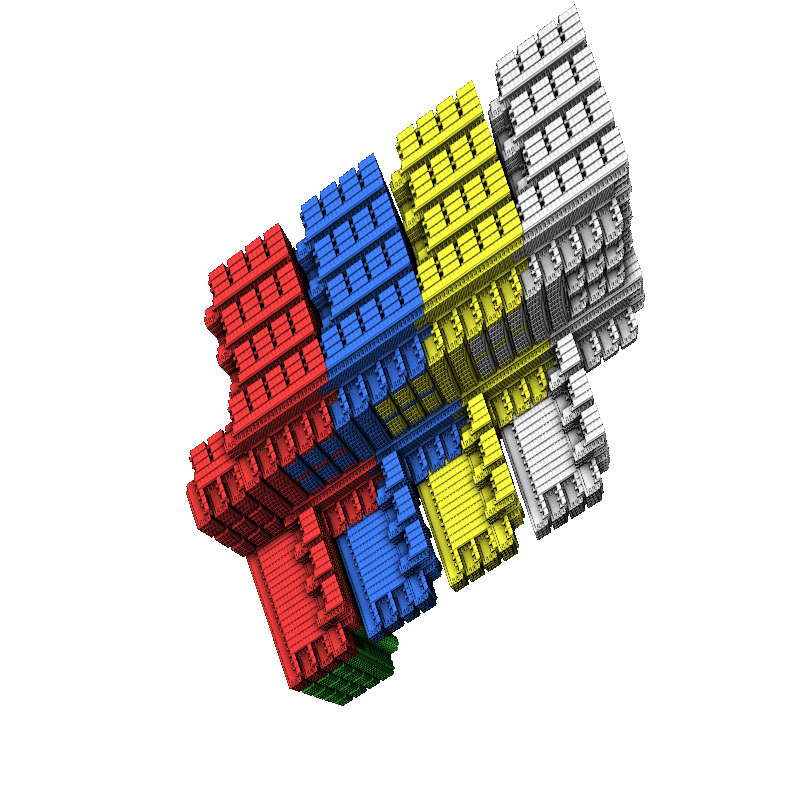
\includegraphics[width=0.5\textwidth]{comb3d_n5.png}
\caption{The $3$-dimensional comb tile $C_5^{(3)}$
  ($d = 3$, $n = 5$), rendered in the real Jordan basis of the
  companion matrix $g$ for $x^3 - 5$.}
\label{fig:comb3d}
\end{figure}

\begin{remark}[IFStile program for $d = 3$]\label{rem:aifs-3d}
The $3$-dimensional comb tile can be rendered in
IFStile~\cite{ifstile} using the following program
(shown for $n = 5$):
\begin{verbatim}
@
$dim=3
$subspace=[g,0,1]
g=$companion([-5,0,0])
h1=[4,0,0]
h2=[8,0,0]
h3=[12,0,0]
h4=[19,7,7]*-1
A=g^-1*(1|h1|h2|h3|h4)*A
\end{verbatim}
\noindent
Here \verb|$companion([-5,0,0])| creates the companion matrix
of $x^3 - 5$, and \verb|$subspace=[g,0,1]| projects
from~$\R^3$ to the eigenbasis of~$g$: the real eigenvalue
$5^{1/3}$ (index~$0$, one dimension) and the complex conjugate
pair $5^{1/3}\zeta_3^{\pm 1}$ (index~$1$, two dimensions).
For general $n \ge 3$, replace $-5$ with $-n$ in the companion
matrix, adjust the translations to
$h_j = [j(n{-}1),0,0]$ for $j = 1,\ldots,n{-}2$,
and set $h_{n-1} = [n^2{-}n{-}1,\; 2n{-}3,\; 2n{-}3] \cdot
(-I_3)$.
\end{remark}

% [d=1 closed-form case moved up to its own section between
%  \S\ref{sec:comb} and \S\ref{sec:osc}: see \S\ref{sec:d1}.]

\subsection{Boundary component count}

\begin{theorem}[Boundary components]\label{thm:pieces}
For every $d \ge 1$ and $n \ge 3$, the number $p(d)$ of boundary
components of $C_n^{(d)}$ depends only on~$d$, not on~$n$, and
satisfies the linear recurrence
\begin{equation}\label{eq:pieces-rec}
  p(d) = 2\,p(d{-}1) + p(d{-}2) + 2,
  \qquad d \ge 2,
\end{equation}
with initial values $p(0) = 0$ and $p(1) = 2$
(Proposition~\ref{prop:d1}); equivalently, $p(2) = 6$
(Theorem~\ref{thm:graph}).  The proof is given in
Corollary~\ref{cor:pell}.
\end{theorem}

\begin{table}[h]
\centering
\caption{Boundary component count $p(d)$ and reduced
  characteristic polynomial degree $\deg q_n^{(d)}$ of the
  $d$-dimensional comb tile.  Rows for $d \in \{1, 2\}$ are
  proved directly (Proposition~\ref{prop:d1},
  Theorem~\ref{thm:graph}); rows for $d \ge 3$ are established
  by Corollary~\ref{cor:pell} via
  the letter-level forward-invariance argument of
  Section~\ref{sec:proof-strategy}.}
\label{tab:pieces}
\begin{tabular}{rrrl}
\toprule
$d$ & $p(d)$ & $\deg q_n^{(d)}$ & Status \\
\midrule
1 &     2 &    2 & Proposition~\ref{prop:d1} \\
2 &     6 &    4 & Theorem~\ref{thm:graph}, Theorem~\ref{thm:dim} \\
3 &    16 &   10 & Corollary~\ref{cor:pell} \\
4 &    40 &   24 & Corollary~\ref{cor:pell} \\
5 &    98 &   58 & Corollary~\ref{cor:pell} \\
6 &   238 &  140 & Corollary~\ref{cor:pell} \\
7 &   576 &  338 & Corollary~\ref{cor:pell} \\
\bottomrule
\end{tabular}
\end{table}

The sequence
$(p(d))_{d\ge 0} = 0,\, 2,\, 6,\, 16,\, 40,\, 98,\, 238,\, 576,\,
1392,\, \ldots$
is the Pell-type sequence appearing in OEIS entries
A213667, A265278, and A293004 under different initial
conventions~\cite{oeis-A213667,oeis-A265278,oeis-A293004}.
Solving the recurrence~\eqref{eq:pieces-rec} yields the closed form
\begin{equation}\label{eq:pieces-closed}
  p(d)
  = \tfrac{1}{2}\bigl((1{+}\sqrt{2})^{d+1}
                      + (1{-}\sqrt{2})^{d+1}\bigr) - 1.
\end{equation}
Asymptotically $p(d) \sim (1{+}\sqrt{2})^{d+1}/2$, so the graph
complexity grows exponentially with the ambient dimension but
remains independent of~$n$.

\begin{remark}[Component count and nullity structure]
\label{rem:nullity-structure}
The occurrence of the same small-coefficient recurrence in OEIS is
only used here as an external identifier for the sequence.  The
structural information needed for the boundary graph comes instead
from the substitution matrix:
for $d \in \{2, 3, 4, 5, 6\}$ direct computation gives
$\dim\ker M_n^{(d)} = 2 P_{d-1}$
\textup{(}independent of $n$\textup{)}, where
$P_k$ denotes the $k$-th Pell number
\textup{(}$P_0 = 0$, $P_1 = 1$, $P_2 = 2$, $P_3 = 5$,
$P_4 = 12$, $P_5 = 29$, satisfying $P_k = 2 P_{k-1} + P_{k-2}$\textup{)};
the corresponding $\dim\ker$ values $(2, 4, 10, 24, 58)$ match
$2 P_{d-1}$ exactly\@.  Equivalently, the nullity
satisfies the same Pell recurrence
$K(d) = 2 K(d{-}1) + K(d{-}2)$ as $p(d)$, but \emph{without} the
inhomogeneous $+2$ term in~\eqref{eq:pieces-rec}.  Theorem~\ref{thm:nullity-equal}
proves this holds for every $d \ge 1$.  Thus the characteristic
polynomial is divisible by $t^{2P_{d-1}}$, and removing only the
factor forced by the geometric zero eigenspace leaves a quotient
of degree $p(d) - 2 P_{d-1}$.  This is not the fully reduced
characteristic polynomial when $d \ge 3$: Theorem~\ref{thm:alg-mult-sym}
proves the stronger algebraic statement
$\mathrm{alg.mult}_0(M_n^{(d)})=p(d{-}1)$ for $d \ge 2$, so
division by the full zero-primary factor leaves degree
$p(d)-p(d{-}1)$, equivalently $2 P_d$.  Note that $2 P_{d-1} = p(d{-}1)$ holds
trivially at $d = 1$ (both sides are $0$) and nontrivially at
$d = 2$; the sequences diverge from $d = 3$ onward, so the
geometric and algebraic reductions no longer have the same
degree.
Theorem~\ref{thm:nullity-lower} below establishes the matching
rigorous lower bound $\dim \ker M_n^{(d)} \ge 2 P_{d-1}$ via
an explicit family of $n$-rational kernel vectors $v(\sigma)$
indexed by~$\mathcal{F}(d)$, and Theorem~\ref{thm:nullity-equal}
completes the equality by the Schur-complement upper bound.  An
equivalent reformulation is that the columns of $M_n^{(d)}$
indexed by $\mathcal{N}(d, n) \setminus \mathcal{F}(d)$ are
linearly independent over~$\mathbb{Q}$.
\end{remark}

\paragraph{Proof architecture for the algebraic part.}
The rest of this section separates the algebraic consequences of
the neighbor rule into four layers.  First, Lemmas~\ref{lem:flip-equal-columns}--\ref{lem:iota-equivariance}
construct explicit kernel vectors and prove the basic
$\iota$-equivariance needed to split the plus stratum into
symmetric and anti-symmetric parts.  Second,
Lemmas~\ref{lem:Mmm-block}--\ref{lem:det-Mmm} analyse the
minus block $M_{--}$ and make the Schur complement available.
Third, Lemmas~\ref{lem:reachability}--\ref{lem:nullity-sym}
prove the exact nullity by comparing inactive and active
$\iota$-pairs.  Finally,
Theorem~\ref{thm:abinva} through
Corollary~\ref{prop:smw-similarity-implies-amult} identify the
Schur correction explicitly; this upgrades the geometric nullity
statement to the full algebraic multiplicity of the zero
eigenvalue.

\begin{lemma}[Sign-flip pairs of equal columns]
\label{lem:flip-equal-columns}
Let $\sigma = (+, T_1, \ldots, T_{d-1}, 0) \in \mathcal{N}(d, n)$
be a plus-stratum vertex with $T_{d-1} \neq 0$, and let
$\iota(\sigma) := (+, -T_1, \ldots, -T_{d-1}, 0)$ denote its
sign-flip on $\mathcal{P}_+$.  Then $\iota(\sigma) \in
\mathcal{N}(d, n)$, and the columns of $M_n^{(d)}$ at $\sigma$
and $\iota(\sigma)$ are equal:
\[
  M_n^{(d)}[\tau, \sigma] \;=\; M_n^{(d)}[\tau, \iota(\sigma)]
  \qquad \text{for every } \tau \in \mathcal{N}(d, n) \text{ and every } n \ge 3.
\]
Consequently, $A^{(d)}[\tau, \sigma] = A^{(d)}[\tau, \iota(\sigma)]$
and $B^{(d)}[\tau, \sigma] = B^{(d)}[\tau, \iota(\sigma)]$ for
all~$\tau$, so the difference $e_\sigma - e_{\iota(\sigma)}$ lies
in $\ker A^{(d)} \cap \ker B^{(d)} \subseteq \ker M_n^{(d)}$.
\end{lemma}

\begin{proof}
The plus-stratum local rule of Theorem~\ref{thm:nindep-real} (no
consecutive $(-, +)$ or $(+, -)$) is preserved under the
sign-flip $\iota$, so $\iota(\sigma) \in \mathcal{N}(d, n)$.

We show that the bijection $(k, l) \leftrightarrow (l, k)$ on
$\{0, \ldots, n-1\}^2$ pairs admissible refinements
$\sigma \to \tau$ with admissible refinements
$\iota(\sigma) \to \tau$, with the same target~$\tau$.

The macro-case is~A (parent sign $\varepsilon = +$).  Among the
four sub-cases, A1 ($\varepsilon_k = \varepsilon_l = +1$) and~A4
($\varepsilon_k = \varepsilon_l = -1$) of
Theorem~\ref{thm:bandt-explicit} produce $T'_d = T_{d-1}$ and
$T'_d = -T_{d-1}$ respectively, both forcing $T'_d \in
\{-(n-1),\, n-1\}$ when $T_{d-1} \neq 0$.  Since the child sign
in A1 and A4 is $\varepsilon' = +1$ and a plus-stratum vertex
requires $T'_d = 0$, no admissible child arises in either
sub-case.  Hence only A2 and A3 contribute, and they are
exchanged by $(k, l) \leftrightarrow (l, k)$ (this exchange
swaps which digit equals $n-1$).

In sub-case~A2 on parent $\sigma$ with digits $(k, l) = (n-1, l)$,
$l < n-1$:
\begin{align*}
  T'_i &= T_{i-1} + (2n-3), \qquad i \ge 2,\\
  T'_1 &= (n-1)(n - l) - 1,\\
  \varepsilon' &= -1.
\end{align*}
In sub-case~A3 on parent $\iota(\sigma)$ with digits
$(l, k) = (l, n-1)$, $l < n-1$:
\begin{align*}
  T'_i &= (2n-3) - (-T_{i-1}) = T_{i-1} + (2n-3), \qquad i \ge 2,\\
  T'_1 &= (n-1)(n - l) - 1,\\
  \varepsilon' &= -1.
\end{align*}
The two children coincide.  The admissibility constraints
($T'_d \in \mathcal{Q}_-$) are also identical: in A2 on $\sigma$
the requirement $T'_d \le 2n-3$ excludes $T_{d-1} = n-1$, while
in A3 on $\iota(\sigma)$ it excludes $-T_{d-1} = -(n-1)$, i.e.,
the same value of $T_{d-1}$.  The case A3 on $\sigma$ paired
with A2 on $\iota(\sigma)$ via $(k, l) \leftrightarrow (l, k)$
is symmetric, with $l$ and $k$ interchanged in the formulas.

Hence the multiset of admissible refinements of~$\sigma$
coincides with that of~$\iota(\sigma)$ via the bijection
$(k, l) \leftrightarrow (l, k)$, proving the column equality.
\end{proof}

\begin{definition}[Plus-stratum index set $\mathcal{F}(d)$ and
auxiliary minus-stratum vertices]
\label{def:F-and-psi}
Let
\[
  \mathcal{F}(d) \;:=\; \bigl\{\sigma \in
                    \mathcal{B}_+(d, n) \cap \mathcal{N}(d, n)
                    : T_{d-1} \neq 0\bigr\}.
\]
For each $\sigma = (+, T_1, \ldots, T_{d-1}, 0) \in
\mathcal{F}(d)$, write $T_{d-1} = \varepsilon\,(n-1)$ with
$\varepsilon \in \{\pm 1\}$ and define the bijections
$\rho_+, \rho_- : \mathcal{P}_+ \to \mathcal{P}_-$ by
\[
  \rho_+ : (- \mapsto a,\; 0 \mapsto b,\; + \mapsto c),
  \qquad
  \rho_- : (- \mapsto c,\; 0 \mapsto b,\; + \mapsto a),
\]
and set
\[
  \pi_\sigma := \begin{cases} \rho_+ & \text{if } \varepsilon = -1,\\
                              \rho_- & \text{if } \varepsilon = +1,\end{cases}
  \qquad
  \bar\pi_\sigma := \begin{cases} \rho_- & \text{if } \varepsilon = -1,\\
                                  \rho_+ & \text{if } \varepsilon = +1.\end{cases}
\]
In both cases $\pi_\sigma(T_{d-1}) = a$ and
$\bar\pi_\sigma(T_{d-1}) = c$.  Define three auxiliary
minus-stratum vertices
\begin{align*}
  \psi_a(\sigma) &:= \bigl(-,\, \pi_\sigma(T_1),\, \ldots,\, \pi_\sigma(T_{d-1}),\, a\bigr),\\
  \psi_b(\sigma) &:= \bigl(-,\, \pi_\sigma(T_1),\, \ldots,\, \pi_\sigma(T_{d-1}),\, b\bigr),\\
  \psi_c(\sigma) &:= \bigl(-,\, \bar\pi_\sigma(T_1),\, \ldots,\, \bar\pi_\sigma(T_{d-1}),\, b\bigr).
\end{align*}
\end{definition}

\begin{lemma}[Admissibility of $\psi_a, \psi_b, \psi_c$]
\label{lem:psi-admissibility}
For every $\sigma \in \mathcal{F}(d)$ and every $n \ge 3$:
$\psi_a(\sigma) \in \mathcal{N}(d, n)$ unconditionally;
$\psi_b(\sigma) \in \mathcal{N}(d, n)$ iff $\pi_\sigma(T_1) \neq a$;
$\psi_c(\sigma) \in \mathcal{N}(d, n)$ iff $\pi_\sigma(T_1) \neq c$
\textup{(}equivalently $\bar\pi_\sigma(T_1) \neq a$\textup{)}.
\end{lemma}

\begin{proof}
Both $\rho_+$ and $\rho_-$ map the forbidden plus-stratum
bigrams $\{(-,+), (+,-)\}$ to the forbidden minus-stratum
bigrams $\{(a,c), (c,a)\}$.  Since $\sigma \in \mathcal{N}(d, n)$
avoids the former, the prefixes
$(\pi_\sigma(T_1), \ldots, \pi_\sigma(T_{d-1}))$ and
$(\bar\pi_\sigma(T_1), \ldots, \bar\pi_\sigma(T_{d-1}))$ both
avoid the latter.  The trailing bigrams
$(\pi_\sigma(T_{d-1}), a) = (a, a)$,
$(\pi_\sigma(T_{d-1}), b) = (a, b)$, and
$(\bar\pi_\sigma(T_{d-1}), b) = (c, b)$ are all
M1-admissible.  Hence M1 holds for all three.

The minus-stratum rule M2 forbids $T_1 = a$ together with
$T_d = b$.  $\psi_a$ has $T_d = a$, so M2 is vacuous.
$\psi_b$ has $T_d = b$, so M2 forbids $\pi_\sigma(T_1) = a$.
$\psi_c$ has $T_d = b$, so M2 forbids $\bar\pi_\sigma(T_1) = a$,
which is equivalent to $\pi_\sigma(T_1) = c$.
\end{proof}

\begin{theorem}[Lower bound on the nullity of $M_n^{(d)}$]
\label{thm:nullity-lower}
For every $d \ge 1$ and every $n \ge 3$,
\begin{equation}\label{eq:nullity-lower}
  \dim \ker M_n^{(d)}
  \;\ge\; 2\,P_{d-1},
\end{equation}
matching the value stated in
Remark~\ref{rem:nullity-structure}.  An explicit linearly
independent family in $\ker M_n^{(d)}$ is
\begin{equation}\label{eq:v-sigma}
  v(\sigma) \;:=\; (n-2)\,e_\sigma
                   \;-\; e_{\psi_a(\sigma)}
                   \;-\; e_{\psi_b(\sigma)}
                   \;+\; (n-1)\,e_{\psi_c(\sigma)},
  \qquad \sigma \in \mathcal{F}(d),
\end{equation}
where the basis vectors $e_{\psi_b(\sigma)}$ and
$e_{\psi_c(\sigma)}$ are interpreted as zero whenever the
corresponding vertex is not in $\mathcal{N}(d, n)$.
\end{theorem}

\begin{proof}
\textit{Cardinality.}\
By the same transfer-matrix argument as in
Corollary~\ref{cor:pell}, the number of words
$T \in \{-, 0, +\}^{d-1}$ avoiding $(-, +)$ and $(+, -)$ with
$T_{d-1} \neq 0$ equals $2 g(d-1) = 2 P_{d-1}$, where
$g(k+1) = 2 g(k) + g(k-1)$ with $g(0) = 0$, $g(1) = 1$ is the
Pell recurrence; symmetry $T \mapsto -T$ accounts for the
factor~$2$.  Hence $|\mathcal{F}(d)| = 2 P_{d-1}$.

\smallskip
\textit{Linear independence.}\
The plus-stratum projection of $v(\sigma)$ is $(n-2)\,e_\sigma$.
For $n \ge 3$ this is nonzero, and the projections at distinct
$\sigma \in \mathcal{F}(d)$ are pairwise orthogonal in
$\mathbb{R}^{\mathcal{B}_+(d, n) \cap \mathcal{N}(d, n)}$, so
the family $\{v(\sigma) : \sigma \in \mathcal{F}(d)\}$ is
linearly independent.

\smallskip
\textit{Membership in $\ker M_n^{(d)}$.}\
Fix $\sigma \in \mathcal{F}(d)$ and write $\pi = \pi_\sigma$,
$\bar\pi = \bar\pi_\sigma$.  Define three target minus-stratum
vertices
\[
  \alpha := \bigl(-,\, a,\, \pi(T_1),\, \ldots,\, \pi(T_{d-1})\bigr),\quad
  \beta  := \bigl(-,\, b,\, \pi(T_1),\, \ldots,\, \pi(T_{d-1})\bigr),\quad
  \gamma := \bigl(-,\, c,\, \pi(T_1),\, \ldots,\, \pi(T_{d-1})\bigr),
\]
all of length $d+1$ with $T_d = \pi(T_{d-1}) = a$.  By the same
M1/M2 analysis as Lemma~\ref{lem:psi-admissibility},
$\beta \in \mathcal{N}(d, n)$ unconditionally,
$\gamma \in \mathcal{N}(d, n)$ iff $\pi(T_1) \neq a$, and
$\alpha \in \mathcal{N}(d, n)$ iff $\pi(T_1) \neq c$.
By Lemma~\ref{lem:psi-admissibility} the conditions
$[\gamma \in \mathcal{N}]$ and $[\alpha \in \mathcal{N}]$
coincide respectively with $[\psi_b(\sigma) \in \mathcal{N}]$
and $[\psi_c(\sigma) \in \mathcal{N}]$.

\smallskip
\textit{Step 1: column at $\sigma$.}\
By the analysis already carried out in the proof of
Lemma~\ref{lem:flip-equal-columns}, sub-cases A1 and A4 of
Theorem~\ref{thm:bandt-explicit} contribute no admissible child
for $\sigma$.  Sub-case A2 contributes only when
$\varepsilon = -1$ and sub-case A3 only when $\varepsilon = +1$;
in either case the formulas yield $T'_i = \pi(T_{i-1})$ for
$i \ge 2$ (so $T'_d = \pi(T_{d-1}) = a$) and
$T'_1 \in \{2n-3, 3n-4\} = \{b, c\}$ via the two values of the
free digit ($l$ in A2, $k$ in A3), each with multiplicity~$1$.
The candidate child with $T'_1 = c$ has bigram $(c, \pi(T_1))$,
which is M1-forbidden iff $\pi(T_1) = a$.  Hence
\begin{equation}\label{eq:M-col-sigma}
  M_n^{(d)}\,e_\sigma \;=\; e_\beta \;+\; [\gamma \in \mathcal{N}]\,e_\gamma,
\end{equation}
which is $n$-independent.

\smallskip
\textit{Step 2: column at $\psi_a(\sigma)$.}\
Parent $\psi_a$ has $T_d = a$ and the
plus-stratum-image prefix.  Among the four B-sub-cases of
Theorem~\ref{thm:bandt-explicit}, sub-cases B2 ($k = n-1$,
$l < n-1$) and B3 ($k < n-1$, $l = n-1$) produce the child sign
$\varepsilon' = +1$ together with $T'_d = a - (2n-3) = -(n-1)$
and $T'_d = (2n-3) - a = +(n-1)$ respectively, neither of which
equals~$0$, so no admissible plus-stratum child arises.
Sub-case B4 ($k = l = n-1$) gives $T'_1 = n^2 - 2$, exceeding
$3n - 4$ for $n \ge 3$, hence not in $\mathcal{Q}_-$.

Only sub-case B1 ($k, l \in \{0, \ldots, n-2\}$) contributes.
The B1 formulas read $T'_i = T_{i-1} = \pi(T_{i-1})$ for
$i \ge 2$ (so $T'_d = a$) and
\[
  T'_1 \;=\; n^2 - 2n - (k+l)(n-1)
       \;\in\; \{a,\, b,\, c\}
       \quad\text{for}\quad k+l \in \{n-2,\, n-3,\, n-4\}.
\]
The number of pairs $(k, l) \in \{0, \ldots, n-2\}^2$ with
$k + l = m$ equals $\min(m+1,\, 2n-3-m)$, which evaluated at
$m \in \{n-2, n-3, n-4\}$ gives the multiplicities
$(n-1, n-2, n-3)$ for $T'_1 \in (a, b, c)$.  The candidate
child with $T'_1 = a$ has bigram $(a, \pi(T_1))$, M1-forbidden
iff $\pi(T_1) = c$, i.e., iff $\alpha \notin \mathcal{N}$;
similarly the candidate with $T'_1 = c$ is M1-forbidden iff
$\gamma \notin \mathcal{N}$.  Therefore
\begin{equation}\label{eq:M-col-psia}
  M_n^{(d)}\,e_{\psi_a(\sigma)}
    \;=\; (n-1)\,[\alpha \in \mathcal{N}]\,e_\alpha
       \;+\; (n-2)\,e_\beta
       \;+\; (n-3)\,[\gamma \in \mathcal{N}]\,e_\gamma.
\end{equation}

\smallskip
\textit{Step 3: column at $\psi_b(\sigma)$
\textup{(}only when $\psi_b \in \mathcal{N}$\textup{)}.}\
Parent $\psi_b$ has $T_d = b$.  Sub-cases B2, B3, B4 give
$T'_d \in \{-1, +1\} \cdot (n-1)$ or $T'_d = 2(2n-3) - b = b$ (B4),
none combinable with $T'_d \in \mathcal{Q}_-$ and the M1 rule;
explicit check: B4 yields $T'_1 = 2n^2 - 3n - n \cdot b
= 2n^2 - 3n - n(2n-3) = 0$, not in $\mathcal{Q}_-$.
For B1 with $T_d = b = 2n-3$, the formula
$T'_1 = 2n^2 - 3n - (k+l)(n-1)$ forces $k + l = 2n - 4$ for
$T'_1 \in \mathcal{Q}_-$, giving the unique value $T'_1 = c$
with multiplicity~$1$.  The bigram $(c, \pi(T_1))$ is admissible
iff $\pi(T_1) \neq a$, i.e., iff $\gamma \in \mathcal{N}$.  Thus
\begin{equation}\label{eq:M-col-psib}
  M_n^{(d)}\,e_{\psi_b(\sigma)}
    \;=\; [\gamma \in \mathcal{N}]\,e_\gamma
  \qquad (\psi_b(\sigma) \in \mathcal{N}).
\end{equation}

\smallskip
\textit{Step 4: column at $\psi_c(\sigma)$
\textup{(}only when $\psi_c \in \mathcal{N}$\textup{)}.}\
Parent $\psi_c$ has $T_{d-1} = \bar\pi(T_{d-1}) = c$ and
$T_d = b$.  In sub-case B1, $T'_d = T_{d-1} = c \notin
\mathcal{Q}_-$, so B1 fails; B2 and B3 give
$T'_d \in \{c - (2n-3),\, (2n-3) - c\} = \{-(n-1),\, n-1\}$,
both incompatible with~$\mathcal{Q}_-$.

Sub-case B4 ($k = l = n-1$) yields
$T'_d = 2(2n-3) - c = a \in \mathcal{Q}_-$, child sign
$\varepsilon' = -1$, and
\[
  T'_1 \;=\; 2(n^2 - n - 1) - n \cdot b
       \;=\; 2n^2 - 2n - 2 - n(2n-3)
       \;=\; n - 2 \;=\; a.
\]
For $i \ge 2$, $T'_i = 2(2n-3) - \bar\pi(T_{i-1})$.  The
involution $x \mapsto 2(2n-3) - x$ on $\mathcal{P}_-$ exchanges
$a \leftrightarrow c$ and fixes $b$, hence transforms $\rho_-$
into $\rho_+$ and vice versa.  Therefore
$T'_i = \pi(T_{i-1})$, and the unique B4 child equals
$(-, a, \pi(T_1), \ldots, \pi(T_{d-1})) = \alpha$, with
multiplicity~$1$ and bigram $(a, \pi(T_1))$ M1-admissible iff
$\pi(T_1) \neq c$, i.e., iff $\alpha \in \mathcal{N}$
(which holds by hypothesis $\psi_c \in \mathcal{N}$).  Hence
\begin{equation}\label{eq:M-col-psic}
  M_n^{(d)}\,e_{\psi_c(\sigma)} \;=\; e_\alpha
  \qquad (\psi_c(\sigma) \in \mathcal{N}).
\end{equation}

\smallskip
\textit{Step 5: closing identity.}\
Combining \eqref{eq:M-col-sigma}--\eqref{eq:M-col-psic} with the
definition~\eqref{eq:v-sigma}, and using the convention that
omitted terms vanish exactly when the corresponding vertex is
absent from $\mathcal{N}(d, n)$:
\begin{align*}
  M_n^{(d)}\,v(\sigma)
   &= (n-2)\bigl(e_\beta + [\gamma \in \mathcal{N}]\,e_\gamma\bigr)\\
   &\quad - \bigl((n-1)\,[\alpha \in \mathcal{N}]\,e_\alpha
              + (n-2)\,e_\beta
              + (n-3)\,[\gamma \in \mathcal{N}]\,e_\gamma\bigr)\\
   &\quad - [\gamma \in \mathcal{N}]\,e_\gamma
        + (n-1)\,[\alpha \in \mathcal{N}]\,e_\alpha\\
   &= 0,
\end{align*}
where the three coefficients cancel independently:
$e_\alpha$:\ $-(n-1) + (n-1) = 0$;
$e_\beta$:\ $(n-2) - (n-2) = 0$;
$e_\gamma$:\ $(n-2) - (n-3) - 1 = 0$.
The cancellations hold for every $n \ge 3$ and every choice of
the Iverson conditions (the four cases
$\{\alpha \in \mathcal{N}\} \times \{\gamma \in \mathcal{N}\}$
correspond to selectively dropping vanishing terms).  Hence
$v(\sigma) \in \ker M_n^{(d)}$.

This proves the displayed lower bound on $\dim \ker M_n^{(d)}$.
\end{proof}

\begin{remark}
The vector $e_\sigma - e_{\iota(\sigma)}$ of
Lemma~\ref{lem:flip-equal-columns} can also be recovered from
the $v$-family of Theorem~\ref{thm:nullity-lower}: an
inspection of Definition~\ref{def:F-and-psi} shows that
$\psi_a(\iota(\sigma)) = \psi_a(\sigma)$,
$\psi_b(\iota(\sigma)) = \psi_b(\sigma)$,
$\psi_c(\iota(\sigma)) = \psi_c(\sigma)$ (the maps depend on
$\sigma$ only through $\varepsilon = T_{d-1}/(n-1)$ and the
prefix multiset, both invariant under $\iota$), so
$v(\sigma) - v(\iota(\sigma)) = (n-2)\,(e_\sigma -
e_{\iota(\sigma)})$.  Since $n \ge 3$, the flip-difference lies
in the span of the $v$-family.
\end{remark}

\medskip
\noindent\textit{Equality of nullity: upper bound.}
\label{par:nullity-upper}
We now strengthen Theorem~\ref{thm:nullity-lower} to the
equality
\begin{equation}\label{eq:nullity-equal}
  \dim \ker M_n^{(d)} \;=\; 2\,P_{d-1}
  \qquad (d \ge 1,\ n \ge 3).
\end{equation}
The proof proceeds in four stages: an involution
$\iota$ acting on $\mathcal{N}(d, n)$ commutes with $M_n^{(d)}$
and induces a block decomposition $V = V_+^{\rm anti} \oplus
V_+^{\rm sym} \oplus V_-$
(Lemma~\ref{lem:iota-equivariance});
the minus-block $M_{--}$ is invertible
(Lemma~\ref{lem:det-Mmm}), so a Schur complement reduces the
rank computation to a matrix on $V_+ = V_+^{\rm anti} \oplus
V_+^{\rm sym}$; the anti-block contributes nullity exactly
$P_{d-1}$ via flip-equal-columns
(Lemma~\ref{lem:nullity-anti}); and the symmetric block
contributes nullity exactly $P_{d-1}$ via an explicit
Reachability lemma combined with a shift map
(Lemmas~\ref{lem:reachability}--\ref{lem:nullity-sym}).

\smallskip
\noindent\textit{The involution~$\iota$.}
Extend $\iota$ from
Lemma~\ref{lem:flip-equal-columns} (defined there only on
$\mathcal{B}_+(d, n)$ as sign-flip $T_i \mapsto -T_i$) to all of
$\mathcal{N}(d, n)$ by the identity on $\mathcal{B}_-(d, n)$.
Both the $(-, +)/(+, -)$ rule on $\mathcal{B}_+$ and the M1/M2
rules on $\mathcal{B}_-$ are $\iota$-stable, so $\iota$
restricts to an involution of $\mathcal{N}(d, n)$.

\begin{lemma}[$\iota$-equivariance of $M_n^{(d)}$]
\label{lem:iota-equivariance}
For every $d \ge 1$, $n \ge 3$, and $\sigma, \tau \in
\mathcal{N}(d, n)$,
\begin{equation}\label{eq:iota-equiv}
  M_n^{(d)}[\iota\tau,\, \iota\sigma]
  \;=\; M_n^{(d)}[\tau,\, \sigma].
\end{equation}
Equivalently, the diagonal involution
$P : e_\sigma \mapsto e_{\iota\sigma}$ on
$V := \R^{\mathcal{N}(d, n)}$ satisfies
$P\,M_n^{(d)} = M_n^{(d)}\,P$.
\end{lemma}

\begin{proof}
By definition, $M_n^{(d)}[\tau, \sigma]$ counts pairs
$(k, l) \in \{0, \ldots, n-1\}^2$ for which the refinement
$\sigma \to \tau$ via digits $(k, l)$, given by
\eqref{eq:Tprime-i}--\eqref{eq:eps-prime}, is admissible (i.e.,
the resulting child lies in $\mathcal{N}(d, n)$).
We show that the involution $(k, l) \leftrightarrow (l, k)$
combined with $\iota$ is a bijection between the admissible
pairs for $(\tau, \sigma)$ and those for
$(\iota\tau, \iota\sigma)$.

Write $\mathrm{ch}(\sigma; k, l) := (\varepsilon', T')$ for the
formally computed child via
\eqref{eq:Tprime-i}--\eqref{eq:eps-prime} (no admissibility
check yet).  We claim the universal identity
\begin{equation}\label{eq:ch-iota}
  \mathrm{ch}(\iota\sigma;\, l,\, k)
  \;=\; \iota\bigl(\mathrm{ch}(\sigma;\, k,\, l)\bigr).
\end{equation}
The four macro-cases of
Theorem~\ref{thm:bandt-explicit} are checked componentwise.

\smallskip
\textit{Case A → A} \emph{(both children plus-stratum,
$\varepsilon_l = \varepsilon_k$).}\
For $i \ge 2$, the right-hand side of~\eqref{eq:ch-iota} reads
$-T'_i = -\varepsilon_l(\varepsilon\, d_{k, i} + T_{i-1}
- d_{l, i}) = \varepsilon_k(d_{l, i} - T_{i-1} - d_{k, i})$
(using $\varepsilon = +1$ in macro-case~A and
$\varepsilon_l = \varepsilon_k$).  The left-hand side reads
$\varepsilon_k(\varepsilon\, d_{l, i} + (-T_{i-1}) - d_{k, i})
= \varepsilon_k(d_{l, i} - T_{i-1} - d_{k, i})$, which is
identical.  At $i = 1$, the same computation with $n T_d$ in
place of $T_{i-1}$ and $T_d = 0$ on macro-case~A gives both
sides equal to $\varepsilon_k(d_{l, 1} - d_{k, 1})$.  The sign
formula~\eqref{eq:eps-prime} is symmetric in $(k, l) \mapsto
(l, k)$ when $\varepsilon_k = \varepsilon_l$.

\smallskip
\textit{Case A → B} \emph{(plus-stratum to minus-stratum,
$\varepsilon_l = -\varepsilon_k$).}\
The child lies in $\mathcal{B}_-(d, n)$ where $\iota$ acts as
the identity, so~\eqref{eq:ch-iota} reduces to
$\mathrm{ch}(\iota\sigma; l, k) = \mathrm{ch}(\sigma; k, l)$.
For $i \ge 2$, $\mathrm{ch}(\sigma; k, l)_i = \varepsilon_l(d_{k, i}
+ T_{i-1} - d_{l, i})$ and $\mathrm{ch}(\iota\sigma; l, k)_i
= \varepsilon_k(d_{l, i} - T_{i-1} - d_{k, i})
= -\varepsilon_k(d_{k, i} + T_{i-1} - d_{l, i})
= \varepsilon_l(d_{k, i} + T_{i-1} - d_{l, i})$, equal.  The
$i = 1$ component coincides by the same identity with $n T_d
= 0$ (macro-case A); the sign $\varepsilon' = \varepsilon_l \cdot
\varepsilon \cdot \varepsilon_k = -1$ is invariant.

\smallskip
\textit{Case B → A} \emph{(minus-stratum parent;
$\iota$ acts as identity on $\sigma$ and as sign-flip on the
plus-stratum child).}\
Required identity: $-\mathrm{ch}(\sigma; k, l)_i =
\mathrm{ch}(\sigma; l, k)_i$.  Substituting $\varepsilon = -1$:
$-\varepsilon_l(-d_{k, i} + T_{i-1} - d_{l, i})
= \varepsilon_l(d_{k, i} + d_{l, i} - T_{i-1})$, matching
$\varepsilon_k(-d_{l, i} + T_{i-1} - d_{k, i})
= -\varepsilon_k(d_{l, i} + d_{k, i} - T_{i-1})
= \varepsilon_l(d_{l, i} + d_{k, i} - T_{i-1})$ since
$\varepsilon_l = -\varepsilon_k$ for case B → A.  At $i = 1$,
substitute $n T_d \in n \mathcal{Q}_-$ in place of $T_{i-1}$;
the same identity holds.

\smallskip
\textit{Case B → B} \emph{(both minus-stratum,
$\varepsilon_l = \varepsilon_k$, $\iota = \mathrm{id}$ on both
sides).}\
Required: $\mathrm{ch}(\sigma; k, l) = \mathrm{ch}(\sigma; l, k)$.
Substituting $\varepsilon = -1$:
$\mathrm{ch}(\sigma; k, l)_i = \varepsilon_l(-d_{k, i} + T_{i-1}
- d_{l, i})$, symmetric in $(k, l)$ under
$\varepsilon_l = \varepsilon_k$.

\smallskip
This proves~\eqref{eq:ch-iota}.  Both children
$\mathrm{ch}(\sigma; k, l)$ and
$\mathrm{ch}(\iota\sigma; l, k) = \iota(\mathrm{ch}(\sigma; k, l))$
are admissible together since $\iota$ preserves $\mathcal{N}(d, n)$,
proving~\eqref{eq:iota-equiv}.
\end{proof}

\begin{remark}
Lemma~\ref{lem:flip-equal-columns} is the specialisation of
\eqref{eq:iota-equiv} to plus-stratum $\sigma$ with
$T_{d-1} \neq 0$ \emph{combined} with the additional fact that
sub-cases A1, A4 (the only ones that could give a plus-stratum
child of $\sigma$) produce $T'_d = \pm T_{d-1} \neq 0$,
ruling out admissibility.  Hence
$M_n^{(d)} e_\sigma = M_n^{(d)} e_{\iota\sigma}$ for inactive
$\sigma$ (not just $M[\iota \tau, \iota\sigma] = M[\tau, \sigma]$).
\end{remark}

\smallskip
\noindent\textit{Block decomposition.}\
Set $V_+ := \R^{\mathcal{B}_+(d, n) \cap \mathcal{N}(d, n)}$ and
$V_- := \R^{\mathcal{B}_-(d, n)}$, so $V = V_+ \oplus V_-$.  The
involution $\iota$ acts on $V_+$ with $\pm 1$-eigenspaces
$V_+^{\rm sym}$ and $V_+^{\rm anti}$ (spanned respectively by
$e_\sigma + e_{\iota\sigma}$ and $e_\sigma - e_{\iota\sigma}$
over $\iota$-pair representatives) and as the identity on $V_-$
(so $V_-^{\rm anti} = 0$).
Lemma~\ref{lem:iota-equivariance} implies that $M_n^{(d)}$
preserves the $\pm 1$-eigenspaces of $P$, giving
\begin{equation}\label{eq:M-decomp}
  M_n^{(d)} \;=\; M_n^{(d)}\big|_{V_+^{\rm anti}}
              \;\oplus\; \widetilde M_n^{(d)},
\end{equation}
where $\widetilde M_n^{(d)} := M_n^{(d)}\big|_{V_+^{\rm sym}
\oplus V_-}$.  In block form on $V_+^{\rm sym} \oplus V_-$,
$\widetilde M_n^{(d)} = \begin{pmatrix}
M_{++}^{\rm sym} & M_{+-}^{\rm sym} \\
M_{-+}^{\rm sym} & M_{--}
\end{pmatrix}$, where $M_{+-}^{\rm sym}$ is $M_{+-}$ followed by
the projection onto $V_+^{\rm sym}$ (which is identity since
$\iota_+ M_{+-} = M_{+-}$ from $\iota|_{V_-} = \mathrm{id}$ and
\eqref{eq:iota-equiv}), and similarly $M_{-+}^{\rm sym}$ is the
restriction of $M_{-+}$ to $V_+^{\rm sym}$ (its restriction to
$V_+^{\rm anti}$ vanishes by the same argument).


% ==========================================================================
% ==========================================================================
\subsection{Bandt-candidate set in higher dimensions}
\label{sec:bandt}

Throughout this paper we work with the $d$-dimensional comb IFS
$C_n^{(d)}$ defined in Section~\ref{sec:higherdim}.
We follow the notation of the main paper without further comment.
This first section establishes the explicit structure of the
Bandt-candidate set $\mathcal{B}(d, n)$ in arbitrary dimension.

A refined structural property of the neighbor graph is that
the geometric offsets of its vertices, although their integer
entries grow linearly with~$n$, are organised by a finite list
of \emph{universal polynomials in~$n$} that does not depend on
the ambient dimension~$d$, and in fact arrange into an explicit
product structure whose cardinality is $3^d - 1$.

We write
\begin{equation}\label{eq:offset-alphabet}
  \mathcal{P}(n) \;=\; \bigl\{\, -(n{-}1),\; 0,\; n{-}2,\; n{-}1,\;
                                  2n{-}3,\; 3n{-}4 \,\bigr\}
  \;\subset\; \Z,
\end{equation}
and decompose $\mathcal{P}(n)$ into the three strata
\[
  \mathcal{P}_+(n) = \{-(n{-}1),\, 0,\, n{-}1\},\qquad
  \mathcal{P}_-(n) = \{n{-}2,\, 2n{-}3,\, 3n{-}4\},\qquad
  \mathcal{Q}_-(n) = \{n{-}2,\, 2n{-}3\}
\]
(thus $\mathcal{Q}_-(n) \subset \mathcal{P}_-(n)$ and
$\mathcal{P}_+(n) \cap \mathcal{P}_-(n) = \emptyset$).
At $n = 3$ these specialise to
$\mathcal{P}_+(3) = \{-2, 0, 2\}$, $\mathcal{P}_-(3) = \{1, 3, 5\}$,
$\mathcal{Q}_-(3) = \{1, 3\}$.

\begin{definition}[Bandt-candidate set]\label{def:bandt-set}
Let $\mathcal{B}(d, n)$ denote the set of non-identity pairs
$(S, T) \in \{\pm I\} \times \Z^d$ obtained from the
identity~$(I, 0)$ by iterated application of the
refinement rule of Subsection~\ref{ssec:neighbor-formalism} (in dimension~$d$,
with the digit system of Definition~\ref{def:comb-d}),
subject to the coordinate-wise admissibility box induced by
Lemma~\ref{lem:bound}:
\begin{equation}\label{eq:admbox}
  \begin{aligned}
    S = +I:\quad & T_i \in [-(2n{-}3),\, 2n{-}3]\ \ (i<d), \quad
                   T_d \in [-(n{-}2),\, n{-}2],\\
    S = -I:\quad & T_i \in [0,\, 2(2n{-}3)]\ \ (i<d), \quad
                   T_d \in [0,\, 2n{-}3].
  \end{aligned}
\end{equation}
Since every neighbor satisfies~\eqref{eq:admbox} (the tile lies in
$R_d = [0, 2n{-}3]^{d-1} \times [0, n{-}1{-}1/n]$ by
Lemma~\ref{lem:bound}), the actual neighbor set is
contained in $\mathcal{B}(d, n)$.
\end{definition}

\begin{theorem}[Explicit Bandt-candidate set]\label{thm:bandt-explicit}
For every $d \ge 1$ and $n \ge 3$,
\begin{equation}\label{eq:bandt-explicit}
  \mathcal{B}(d, n) \;\subseteq\;
  \underbrace{\bigl\{(+I, T) : T \in
                 \mathcal{P}_+(n)^{d-1} \times \{0\},\ T \neq 0\bigr\}}_{=:\,\mathcal{B}_+(d, n)}
  \;\sqcup\;
  \underbrace{\bigl\{(-I, T) : T \in
                 \mathcal{P}_-(n)^{d-1} \times \mathcal{Q}_-(n)\bigr\}}_{=:\,\mathcal{B}_-(d, n)},
\end{equation}
and the cardinalities $|\mathcal{B}_+(d, n)| = 3^{d-1} - 1$,
$|\mathcal{B}_-(d, n)| = 2 \cdot 3^{d-1}$ add up to $3^d - 1$.
\end{theorem}

\begin{proof}
Set $\mathcal{S}(d, n) := \mathcal{B}_+(d, n) \sqcup \mathcal{B}_-(d, n)
\sqcup \{(I, 0)\}$.  We show that $\mathcal{S}(d, n)$ is closed under
admissible refinement: if $\sigma = (\varepsilon, T) \in \mathcal{S}(d, n)$
and $\sigma' = (\varepsilon', T')$ is an admissible child of $\sigma$
via digit indices $(k, l) \in \{0, \ldots, n-1\}^2$, then
$\sigma' \in \mathcal{S}(d, n)$.  Since $(I, 0) \in \mathcal{S}(d, n)$
generates the closure $\mathcal{B}(d, n) \cup \{(I, 0)\}$, this
yields the inclusion~\eqref{eq:bandt-explicit}.

Recall the digit data: $d_{j, 1} = j(n-1)$ and $d_{j, i} = 0$
($i \ge 2$) for $j < n-1$; $d_{n-1, 1} = n^2 - n - 1$ and
$d_{n-1, i} = 2n-3$ ($i \ge 2$); the signs are $\varepsilon_j = +1$
for $j < n-1$ and $\varepsilon_{n-1} = -1$.  The refinement rule
gives
\begin{align}
  T'_i &= \varepsilon_l\bigl(\varepsilon\, d_{k, i} + T_{i-1}
           - d_{l, i}\bigr), \qquad i \ge 2, \label{eq:Tprime-i}\\
  T'_1 &= \varepsilon_l\bigl(\varepsilon\, d_{k, 1} + n\, T_d
           - d_{l, 1}\bigr), \label{eq:Tprime-1}\\
  \varepsilon' &= \varepsilon_l \cdot \varepsilon \cdot \varepsilon_k.
       \label{eq:eps-prime}
\end{align}
The crucial observation is that the right-hand side
of~\eqref{eq:Tprime-i} depends on $(k, l)$ only through the signs
$(\varepsilon_k, \varepsilon_l)$, since $d_{k, i}$ for $i \ge 2$
takes the two values $0$ (if $k < n-1$) or $2n-3$ (if $k = n-1$).
Throughout the proof we abbreviate
$\mathcal{P}_+ = \{-(n-1), 0, n-1\}$,
$\mathcal{P}_- = \{n-2, 2n-3, 3n-4\}$,
$\mathcal{Q}_- = \{n-2, 2n-3\}$.

\smallskip\noindent\textbf{Macro-case A: parent
$\sigma \in \mathcal{B}_+(d, n) \cup \{(I, 0)\}$.}
Then $\varepsilon = +1$, $T_d = 0$, and $T_i \in \mathcal{P}_+ \cup \{0\}$
for $1 \le i \le d-1$ (the value $0$ is allowed only when
$\sigma = (I, 0)$, in which case all $T_i = 0$).

\emph{A1: $\varepsilon_k = \varepsilon_l = +1$ ($k, l < n-1$).}
By~\eqref{eq:Tprime-i}, $T'_i = T_{i-1} \in \mathcal{P}_+ \cup \{0\}$
for $i \ge 2$.  By~\eqref{eq:Tprime-1}, $T'_1 = (k - l)(n-1)$;
the sign~\eqref{eq:eps-prime} is $\varepsilon' = +1$, so admissibility
demands $|T'_1| \le 2n-3$, forcing $|k - l| \le 1$ and
$T'_1 \in \mathcal{P}_+$.  At $i = d$ the bound $|T'_d| \le n-2$
on a sign-$+I$ child forces $T_{d-1} = 0$ (when $d \ge 2$) or
$k = l$ (when $d = 1$).  Hence $T' \in \mathcal{P}_+^{d-1} \times \{0\}$,
so $\sigma' \in \mathcal{B}_+(d, n) \cup \{(I, 0)\}$.

\emph{A2: $\varepsilon_k = -1$, $\varepsilon_l = +1$ ($k = n-1$,
$l < n-1$).}
Then~\eqref{eq:Tprime-i} gives $T'_i = T_{i-1} + (2n-3)$, mapping
$\mathcal{P}_+ \to \{n-2, 2n-3, 3n-4\} = \mathcal{P}_-$.  The
sign is $\varepsilon' = -1$, and~\eqref{eq:Tprime-1} reads
\[
  T'_1 = (n-1)(n - l) - 1.
\]
For $d \ge 2$, the admissibility bound $T'_1 \le 2(2n-3) = 4n-6$
gives $(n-1)(n-l) \le 4n-5$, i.e., $n - l \le 3$, so
$l \in \{n-3, n-2\}$ and $T'_1 \in \{3n-4, 2n-3\} \subset \mathcal{P}_-$.
For $d = 1$, the tighter bound $T'_1 \le 2n-3$ forces $l = n-2$
and $T'_1 = 2n-3 \in \mathcal{Q}_-$.
At $i = d \ge 2$, $T'_d = T_{d-1} + (2n-3) \in \{n-2, 2n-3, 3n-4\}$;
admissibility $T'_d \le 2n-3$ excludes $T_{d-1} = n-1$, leaving
$T'_d \in \mathcal{Q}_-$.  Thus $\sigma' \in \mathcal{B}_-(d, n)$.

\emph{A3: $\varepsilon_k = +1$, $\varepsilon_l = -1$ ($k < n-1$,
$l = n-1$).}
Then $T'_i = (2n-3) - T_{i-1}$ for $i \ge 2$, mapping $\mathcal{P}_+ \to
\mathcal{P}_-$, and $\varepsilon' = -1$.  Equation~\eqref{eq:Tprime-1}
reads $T'_1 = (n-1)(n-k) - 1$, identical in form to~A2 with $k$ replacing $l$.
The same admissibility analysis yields $k \in \{n-3, n-2\}$ and
$T'_1 \in \{3n-4, 2n-3\}$ for $d \ge 2$, or $k = n-2$ and
$T'_1 = n - 2$ for $d = 1$.  At $i = d \ge 2$, $T'_d = (2n-3) - T_{d-1}$
forces $T_{d-1} \neq -(n-1)$ and $T'_d \in \mathcal{Q}_-$.  Thus
$\sigma' \in \mathcal{B}_-(d, n)$.

\emph{A4: $\varepsilon_k = \varepsilon_l = -1$ ($k = l = n-1$).}
Then $T'_i = -T_{i-1} \in \mathcal{P}_+$ for $i \ge 2$, $\varepsilon' = +1$,
and $T'_1 = 0$.  At $i = d \ge 2$, $|T'_d| = |T_{d-1}| \le n-2$ forces
$T_{d-1} = 0$.  Hence $T' \in \mathcal{P}_+^{d-1} \times \{0\}$ and
$\sigma' \in \mathcal{B}_+(d, n) \cup \{(I, 0)\}$.

\smallskip\noindent\textbf{Macro-case B: parent
$\sigma \in \mathcal{B}_-(d, n)$.}
Then $\varepsilon = -1$, $T_d \in \mathcal{Q}_-$, and
$T_i \in \mathcal{P}_-$ for $1 \le i \le d-1$.

\emph{B1: $\varepsilon_k = \varepsilon_l = +1$.}
$T'_i = T_{i-1} \in \mathcal{P}_-$ for $i \ge 2$, $\varepsilon' = -1$,
and~\eqref{eq:Tprime-1} reads $T'_1 = n T_d - (k+l)(n-1)$.
\begin{itemize}
\item $T_d = n - 2$: $T'_1 = n^2 - 2n - (k+l)(n-1)$.  For $d \ge 2$,
admissibility $T'_1 \in [0, 4n-6]$ forces $k + l \in \{n-4, n-3, n-2\}$
(intersected with the feasible range $[0, 2n-4]$), and the
corresponding values $T'_1 \in \{3n-4, 2n-3, n-2\}$ all lie in
$\mathcal{P}_-$.  For $d = 1$, the tighter bound $T'_1 \le 2n-3$
forces $k+l \in \{n-3, n-2\}$ and $T'_1 \in \mathcal{Q}_-$.
\item $T_d = 2n - 3$: $T'_1 = 2n^2 - 3n - (k+l)(n-1)$.  For $d \ge 2$,
admissibility forces $k + l \ge 2n - 4$, but $k + l \le 2n - 4$ since
$k, l \le n-2$; hence $k + l = 2n - 4$ and $T'_1 = 3n - 4 \in \mathcal{P}_-$.
For $d = 1$, the bound $T'_1 \le 2n-3$ rules out every feasible $(k, l)$.
\end{itemize}
At $i = d \ge 2$, $T'_d = T_{d-1} \in \mathcal{P}_-$; admissibility
$T'_d \le 2n - 3$ excludes $T_{d-1} = 3n - 4$, giving
$T'_d \in \mathcal{Q}_-$.  Thus $\sigma' \in \mathcal{B}_-(d, n)$.

\emph{B2: $\varepsilon_k = -1$, $\varepsilon_l = +1$ ($k = n-1$,
$l < n-1$).}
$T'_i = T_{i-1} - (2n-3) \in \mathcal{P}_+$ for $i \ge 2$,
$\varepsilon' = +1$, and~\eqref{eq:Tprime-1} reads
$T'_1 = -(n^2 - n - 1) + n T_d - l(n-1)$.
Substituting $T_d = n-2$ gives $T'_1 = -(l+1)(n-1)$, and admissibility
$|T'_1| \le 2n-3$ forces $l = 0$, $T'_1 = -(n-1) \in \mathcal{P}_+$.
Substituting $T_d = 2n-3$ gives $T'_1 = (n-1)(n - 1 - l)$, and
admissibility forces $l = n-2$, $T'_1 = n-1 \in \mathcal{P}_+$.
At $i = d \ge 2$, $T'_d = T_{d-1} - (2n-3) \in \mathcal{P}_+$ with
$|T'_d| \le n-2$ forces $T'_d = 0$, i.e., $T_{d-1} = 2n-3$.
Thus $\sigma' \in \mathcal{B}_+(d, n)$.

\emph{B3: $\varepsilon_k = +1$, $\varepsilon_l = -1$ ($k < n-1$,
$l = n-1$).}
$T'_i = (2n-3) - T_{i-1} \in \mathcal{P}_+$ for $i \ge 2$,
$\varepsilon' = +1$, and $T'_1 = k(n-1) - n T_d + (n^2 - n - 1)$.
Substituting $T_d = n-2$: $T'_1 = (k+1)(n-1)$, forcing $k = 0$ and
$T'_1 = n-1 \in \mathcal{P}_+$.
Substituting $T_d = 2n-3$: $T'_1 = (n-1)(k - n + 1)$, forcing $k = n-2$
and $T'_1 = -(n-1) \in \mathcal{P}_+$.
At $i = d \ge 2$, $T'_d = (2n-3) - T_{d-1} \in \mathcal{P}_+$ with
$|T'_d| \le n-2$ forces $T'_d = 0$.  Thus $\sigma' \in \mathcal{B}_+(d, n)$.

\emph{B4: $\varepsilon_k = \varepsilon_l = -1$ ($k = l = n-1$).}
$T'_i = 2(2n-3) - T_{i-1}$ maps $\mathcal{P}_- \to \mathcal{P}_-$
($n-2 \leftrightarrow 3n-4$, $2n-3 \leftrightarrow 2n-3$);
$\varepsilon' = -1$ and~\eqref{eq:Tprime-1} reads
$T'_1 = 2(n^2 - n - 1) - n T_d$.
Substituting $T_d = n-2$ gives $T'_1 = n^2 - 2 > 4n - 6$ for $n \ge 3$
(since $(n - 2)^2 > 0$), violating admissibility; no admissible child.
Substituting $T_d = 2n-3$ gives $T'_1 = n - 2 \in \mathcal{Q}_-
\subset \mathcal{P}_-$ (admissible in either bound).
At $i = d \ge 2$, $T'_d = 2(2n-3) - T_{d-1}$ with $T_{d-1} \in
\mathcal{P}_-$ gives $T'_d \in \{n-2,\ 2n-3,\ 3n-4\}$ for
$T_{d-1} \in \{3n-4,\ 2n-3,\ n-2\}$ respectively; the admissibility
requirement $T'_d \in \mathcal{Q}_-$, i.e.\ $T'_d \le 2n-3$, rules
out $T_{d-1} = n - 2$ and retains both $T_{d-1} = 2n - 3$
(giving $T'_d = 2n - 3$) and $T_{d-1} = 3n - 4$ (giving $T'_d =
n - 2$).  In either case $T'_d \in \mathcal{Q}_-$, so
$\sigma' \in \mathcal{B}_-(d, n)$.

\smallskip
In each of the eight sub-cases, the admissibility box on
$(T'_1, T'_d)$ alone constrains the digit indices and the parent's
last coordinate $T_d$ enough to place $\sigma'$ in $\mathcal{S}(d, n)$.
Hence $\mathcal{S}(d, n)$ is closed under admissible refinement, and
\eqref{eq:bandt-explicit} follows.
The cardinalities $|\mathcal{B}_+| = 3^{d-1} - 1$ and
$|\mathcal{B}_-| = 2 \cdot 3^{d-1}$ are immediate from the product
structure of the right-hand side.
\end{proof}

\medskip
\begin{remark}[Cubic-lattice interpretation of the bound $3^d - 1$]
\label{rem:cube-bound}
The cardinality $|\mathcal{B}(d, n)| = 3^d - 1$ coincides with the
number of face- and corner-adjacent neighbors of a unit cube
$[0, 1]^d$ in the lattice tiling of $\R^d$ by axis-aligned cubes:
each lattice neighbor is parametrised by a non-zero vector
$(\delta_1, \ldots, \delta_d) \in \{-1, 0, +1\}^d$.
The match is structural rather than coincidental.  Under the
projection that sends each coordinate $T_i$ to its
$\mathcal{P}_\pm$-stratum, the splitting
$\mathcal{B}(d, n) =
\mathcal{B}_+(d, n) \sqcup \mathcal{B}_-(d, n)$ of
Theorem~\ref{thm:bandt-explicit} becomes the product
$\bigl(\{-1, 0, +1\}^{d-1} \times \{0\}\bigr) \setminus\{0\}
\sqcup \bigl(\{-1, 0, +1\}^{d-1} \times \{-1, +1\}\bigr)$,
i.e.\ the partition of cube-lattice neighbors by the value of
their last coordinate.  This is the algebraic shadow of the
geometric fact that the bounding parallelepiped~$R_d$
is itself
a $d$-dimensional box: its lattice-of-translates neighbor set has
cardinality $3^d - 1$, and the comb tile $C_n^{(d)} \subset R_d$
inherits this combinatorial bound through the admissibility
box~\eqref{eq:admbox}.  In particular, no comb tile can have more
than $3^d - 1$ neighbor types regardless of~$n$, while the actual
count $p(d)$ \textup{(}Theorem~\ref{thm:pieces},
OEIS A265278\textup{)} grows only as
$\sim (1{+}\sqrt{2})^{d+1}/2 \approx (2.414)^{d+1}/2$,
strictly slower than $3^d$.
\end{remark}

\begin{figure}[ht]
\centering
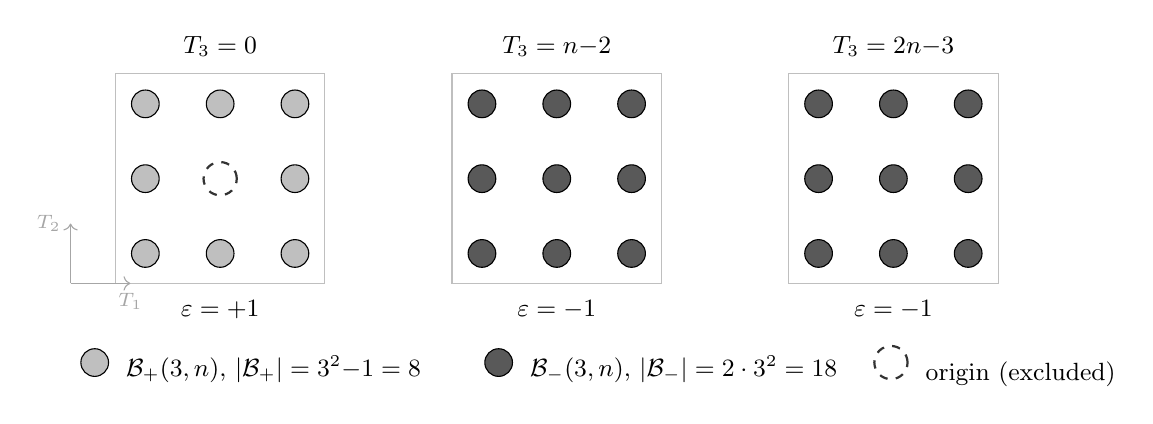
\begin{tikzpicture}[
  scale=0.95,
  Bplus/.style ={circle,draw=black,fill=black!25,minimum size=10pt,inner sep=0pt},
  Bminus/.style={circle,draw=black,fill=black!65,minimum size=10pt,inner sep=0pt},
  hole/.style  ={circle,draw=black!80,dashed,thick,fill=white,minimum size=12pt,inner sep=0pt},
  layer/.style ={draw=gray!50,thin}]
% --- Three 2D slices side by side, each a 3x3 grid in (T_1, T_2) ---
\foreach \cx/\lab/\sign/\type in
  {0/{$T_3=0$}/{$\varepsilon=+1$}/1,
   4.5/{$T_3=n{-}2$}/{$\varepsilon=-1$}/2,
   9/{$T_3=2n{-}3$}/{$\varepsilon=-1$}/2}
{
  % bounding box around each layer
  \draw[layer] (\cx-1.4,-1.4) rectangle (\cx+1.4,1.4);
  % header
  \node[anchor=south] at (\cx,1.5) {\small \lab};
  \node[anchor=north] at (\cx,-1.5) {\small \sign};
  % 3x3 grid of points (numeric loop)
  \foreach \dx in {-1,0,1}
    \foreach \dy in {-1,0,1}
  {
    \ifnum\type=1
      \node[Bplus]  at (\cx+\dx,\dy) {};
    \else
      \node[Bminus] at (\cx+\dx,\dy) {};
    \fi
  }
}
% Overdraw the origin on the plus layer with a clearly distinct dashed hole
\node[hole] at (0,0) {};
% --- Legend across the bottom ---
\node[anchor=west] at (-2.0,-2.5)
  {\small \tikz\node[Bplus]{};~~$\mathcal{B}_+(3,n)$,
   $|\mathcal{B}_+|=3^2{-}1=8$};
\node[anchor=west] at (3.4,-2.5)
  {\small \tikz\node[Bminus]{};~~$\mathcal{B}_-(3,n)$,
   $|\mathcal{B}_-|=2\cdot 3^2=18$};
\node[anchor=west] at (8.6,-2.5)
  {\small \tikz\node[hole]{};~~origin (excluded)};
% --- Coordinate axis hint on first slice ---
\draw[->,gray!70] (-2.0,-1.4) -- (-2.0,-0.6) node[left,font=\scriptsize] {$T_2$};
\draw[->,gray!70] (-2.0,-1.4) -- (-1.2,-1.4) node[below,font=\scriptsize] {$T_1$};
\end{tikzpicture}
\caption{The Bandt-candidate set $\mathcal{B}(3,n)$ of
Theorem~\ref{thm:bandt-explicit} for $d=3$, visualised as three
$3\times 3$ slices indexed by the last coordinate $T_3$.
\textbf{Left:} $T_3=0$, sign $\varepsilon=+1$ --- the $8$ candidates
of $\mathcal{B}_+$ (origin excluded).
\textbf{Middle and right:} $T_3 \in \mathcal{Q}_- = \{n{-}2,\, 2n{-}3\}$,
sign $\varepsilon=-1$ --- the $9 + 9 = 18$ candidates of
$\mathcal{B}_-$.  Total $8 + 18 = 26 = 3^3 - 1$, matching the
cube-lattice neighbor count of $[0,1]^3$.  Under the projection
of Remark~\ref{rem:cube-bound} the three slices correspond to
the three values of the last coordinate of a lattice neighbor
$(\delta_1,\delta_2,\delta_3) \in \{-1,0,+1\}^3 \setminus \{0\}$.}
\label{fig:bandt-d3}
\end{figure}

\begin{corollary}[Polynomial-offset alphabet, every dimension]
\label{cor:poly-offsets}
For every $d \ge 1$ and $n \ge 3$, every neighbor type of the
comb tile $C_n^{(d)}$ is of the form $\sigma(x) = \pm x + t$
with $t \in \mathcal{P}(n)^d$ (the alphabet
of~\eqref{eq:offset-alphabet}).  The integer coefficients of
the six polynomial offsets lie in $\{-4, -3, -2, -1, 0, 1, 2, 3\}$.
\end{corollary}

\begin{proof}
Every neighbor lies in $\mathcal{B}(d, n)$, and by
Theorem~\ref{thm:bandt-explicit} every element of
$\mathcal{B}(d, n)$ has every coordinate in
$\mathcal{P}_+(n) \cup \mathcal{P}_-(n) \cup \{0\}
\subseteq \mathcal{P}(n)$.
\end{proof}

\begin{remark}[Link to Theorem~\ref{thm:pieces}]
\label{rem:bandt-link}
Theorem~\ref{thm:bandt-explicit} bounds $p(d) \le 3^d - 1$
uniformly in~$n$.  The actual neighbor set is a strict subset of
$\mathcal{B}(d, n)$ for $d \ge 2$
(see Theorem~\ref{thm:graph}).
Since the right-hand side of~\eqref{eq:bandt-explicit} is
independent of~$n$, Theorem~\ref{thm:bandt-explicit} implies
Theorem~\ref{thm:pieces} once one shows that
the actual neighbor selection is also $n$-independent.
The next two sections carry out precisely this step: we state an
$n$-independent letter-level filter on $\mathcal{B}(d, n)$
\textup{(}Subsection~\ref{sec:nindep-real}\textup{)}, prove it in
Section~\ref{sec:proof-strategy}
\textup{(}Theorem~\ref{thm:nindep-real}\textup{)},
and derive from it the Pell closed form for $p(d)$
\textup{(}Subsection~\ref{sec:pell}\textup{)}.
\end{remark}

% ==========================================================================
\subsection{An $n$-independent real-neighbor selection rule}
\label{sec:nindep-real}

By Theorem~\ref{thm:bandt-explicit}, every Bandt-candidate vertex
$\sigma = (\varepsilon, T) \in \mathcal{B}(d, n)$ has every
coordinate $T_i$ valued in one of the three-letter strata
$\mathcal{P}_+(n)$ or $\mathcal{P}_-(n)$.  This suggests a
\emph{letter encoding} of $\mathcal{B}(d, n)$ that completely
separates the combinatorial type of $\sigma$ from its arithmetic
realisation in $\Z^d$.

\begin{definition}[Letter encoding of $\mathcal{B}(d, n)$]
\label{def:letters}
For $n \ge 3$, identify
\begin{align*}
  \mathcal{P}_+(n) &= \{-(n{-}1),\, 0,\, n{-}1\}
  \;\longleftrightarrow\; \{-,\, 0,\, +\}, \\
  \mathcal{P}_-(n) &= \{n{-}2,\, 2n{-}3,\, 3n{-}4\}
  \;\longleftrightarrow\; \{a,\, b,\, c\}, \\
  \mathcal{Q}_-(n) &= \{n{-}2,\, 2n{-}3\}
  \;\longleftrightarrow\; \{a,\, b\}.
\end{align*}
Under these bijections, by Theorem~\ref{thm:bandt-explicit}
the splitting $\mathcal{B}(d, n) = \mathcal{B}_+(d, n) \sqcup
\mathcal{B}_-(d, n)$ becomes
\begin{align*}
  \mathcal{B}_+(d, n) &\;\longleftrightarrow\;
    \bigl\{(+, T) : T \in \{-, 0, +\}^{d-1} \times \{0\},\
                    T \neq 0\bigr\},
    \quad |\,\cdot\,| = 3^{d-1} - 1, \\
  \mathcal{B}_-(d, n) &\;\longleftrightarrow\;
    \bigl\{(-, T) : T \in \{a, b, c\}^{d-1} \times \{a, b\}\bigr\},
    \quad |\,\cdot\,| = 2 \cdot 3^{d-1}.
\end{align*}
Both alphabets are independent of~$n$.
\end{definition}

\begin{theorem}[$n$-independent real-neighbor selection]
\label{thm:nindep-real}
Let $\mathcal{N}(d, n) \subseteq \mathcal{B}(d, n)$ denote the set
of real neighbor types of $C_n^{(d)}$.  Under the letter encoding
of Definition~\ref{def:letters},
$\mathcal{N}(d, n)$ depends on $d$ alone and is given by the
following two filters.

\emph{Plus-stratum.}\
A vertex $\sigma = (+, T) \in \mathcal{B}_+(d, n)$ is real if and
only if no consecutive pair $(T_i, T_{i+1})$, $1 \le i \le d-1$,
equals $(-, +)$ or $(+, -)$.

\emph{Minus-stratum.}\
A vertex $\sigma = (-, T) \in \mathcal{B}_-(d, n)$ is real if and
only if both
\begin{enumerate}
  \item[\textup{(M1)}] no consecutive pair $(T_i, T_{i+1})$,
    $1 \le i \le d-1$, equals $(a, c)$ or $(c, a)$
    \textup{(}local-difference rule\textup{)}; and
  \item[\textup{(M2)}] it is not the case that $T_1 = a$ and
    $T_d = b$ \textup{(}endpoint-asymmetry rule\textup{)}.
\end{enumerate}
The proof occupies Section~\ref{sec:proof-strategy}.
\end{theorem}

\begin{remark}[Consistency with the direct low-dimensional computations]
Specialising Theorem~\ref{thm:nindep-real} to $d=1$ and $d=2$
recovers the neighbor lists computed directly in
Proposition~\ref{prop:d1} and Theorem~\ref{thm:graph}.  At $d=1$,
the plus stratum is empty, while the minus stratum is
$\mathcal{Q}_-(n) = \{n{-}2, 2n{-}3\}$; the filters are vacuous
because there are no consecutive pairs and \textup{(M2)} would require
the single coordinate to be both $a$ and $b$.  This gives the two
types $-x+(n{-}2)$ and $-x+(2n{-}3)$ of
Proposition~\ref{prop:d1}.

At $d=2$, the plus stratum gives the two translations
$\pm(n{-}1)$ in the first coordinate, namely $\sigma_1$ and
$\sigma_2$.  The minus stratum is
$\{a,b,c\} \times \{a,b\}$; the rule \textup{(M1)} removes
$(c,a)$ and \textup{(M2)} removes $(a,b)$.  The four surviving
minus types are
\[
  (a,a),\quad (b,a),\quad (b,b),\quad (c,b),
\]
which are respectively $\sigma_6, \sigma_5, \sigma_4, \sigma_3$
in the notation of Theorem~\ref{thm:graph}.
\end{remark}

\begin{remark}[Relation to the SCC characterisation
at $n = 3$]
\label{rem:scc-n3}
At $n = 3$ the letter-encoded bigrams $(-, +)$, $(+, -)$ correspond
to integer differences $|T_i - T_{i+1}| = 4$ in $\{-2, 0, 2\}$,
and the bigrams $(a, c)$, $(c, a)$ correspond to
$|T_i - T_{i+1}| = 4$ in $\{1, 3, 5\}$.  The plus-stratum part
of Theorem~\ref{thm:nindep-real} is therefore the rule
$|T_i - T_{i+1}| \le 2$ on $\{-2, 0, 2\}^{d-1} \times \{0\}$,
and the local rule \textup{(M1)} is the same bound on
$\{1, 3, 5\}^{d-1} \times \{1, 3\}$.  The endpoint-asymmetry
rule \textup{(M2)}, written in the letter alphabet, reads in
$n = 3$ coordinates as ``$T_1 = 1$ and $T_d = 3$ is forbidden''.
Theorem~\ref{thm:nindep-real} is the natural $n$-independent
formulation of this rule via the letter
encoding of Definition~\ref{def:letters}.
\end{remark}

\begin{remark}[Geometric interpretation of \textup{(M2)}]
\label{rem:M2-geometric}
The asymmetric rule \textup{(M2)} reflects the orientation of the
``tooth'' map $h_{n-1}$ in the comb construction
\textup{(}see Section~\ref{sec:higherdim}\textup{)}: the
last-coordinate stratum $\mathcal{Q}_-(n) = \{a, b\}$ is the
\emph{shorter} of the two minus-stratum strata because the tooth
extends in the $+(2n{-}3)$ direction along coordinate~$d$.  A
configuration with $T_1 = a$ at the head of the word $(T_1,
\ldots, T_d)$ corresponds to a translate that the tooth cannot
reach, hence the candidate $(-, a, \ldots, b)$ has empty
intersection with the original tile.  A rigorous combinatorial
proof of~\textup{(M2)} is given by the dead-end argument of
Lemma~\ref{lem:endpoint-dead}.
\end{remark}

% ==========================================================================
\subsection{Algebraic consequence: the Pell recurrence for $p(d)$}
\label{sec:pell}

We now derive the closed-form count of $|\mathcal{N}(d, n)|$ from
Theorem~\ref{thm:nindep-real} by a $3 \times 3$ transfer-matrix
calculation, yielding the Pell-type recurrence
$p(d) = 2 p(d{-}1) + p(d{-}2) + 2$
of Theorem~\ref{thm:pieces}.

The two filters of Theorem~\ref{thm:nindep-real} forbid exactly
the same pair of bigrams: $(-, +)$ and $(+, -)$ on the alphabet
$\{-, 0, +\}$, and $(a, c)$ and $(c, a)$ on the alphabet
$\{a, b, c\}$, with the natural identification
$\{-, 0, +\} \leftrightarrow \{a, b, c\}$.  Both alphabets are
governed by the same $3 \times 3$ \emph{transfer matrix}
\begin{equation}\label{eq:transfer-matrix}
  M \;=\;
  \begin{pmatrix}
    1 & 1 & 0 \\
    1 & 1 & 1 \\
    0 & 1 & 1
  \end{pmatrix}
  \qquad \text{on row/column states } (s_1, s_2, s_3),
\end{equation}
where $M_{ij} = 1$ iff the bigram $(s_i, s_j)$ is admissible
(only the two opposite-extremum bigrams are forbidden).

\begin{lemma}[Spectrum of $M$]\label{lem:spectrum}
The matrix $M$ of \eqref{eq:transfer-matrix} has characteristic
polynomial
\[
  \chi_M(\lambda) \;=\; (\lambda - 1)(\lambda^2 - 2\lambda - 1),
\]
with eigenvalues $\lambda_0 = 1$ and the silver-ratio pair
$\lambda_\pm = 1 \pm \sqrt 2$.  Consequently the Perron root is
$\theta := 1 + \sqrt 2 \approx 2.4142$.
\end{lemma}

\begin{proof}
Direct expansion: $\det(\lambda I - M) = (\lambda - 1)\bigl[(\lambda
- 1)^2 - 2\bigr] = (\lambda - 1)(\lambda^2 - 2\lambda - 1)$.
\end{proof}

Recall the Pell numbers $\Pell(0) = 0$, $\Pell(1) = 1$,
$\Pell(d) = 2\,\Pell(d{-}1) + \Pell(d{-}2)$, sequence
$0, 1, 2, 5, 12, 29, 70, 169, 408, \ldots$, and the half-companion
Pell numbers $H_d := \Pell(d{-}1) + \Pell(d) = (\theta^d
+ \bar\theta^d)/2$ where $\bar\theta = 1 - \sqrt 2$, sequence
$1, 1, 3, 7, 17, 41, 99, 239, 577, \ldots$.  We use the standard
identity
\begin{equation}\label{eq:Hd-identity}
  H_{d+1} \;=\; \Pell(d+1) + \Pell(d)
              \;=\; 2\,\Pell(d) + \Pell(d-1) + \Pell(d)
              \;=\; 3\,\Pell(d) + \Pell(d-1).
\end{equation}

For a length-$d$ word $T = (T_1, \ldots, T_d)$ over the three-letter
alphabet $\{x_1, x_2, x_3\}$, write $T \in \mathcal{W}_d$ to mean
that $T$ avoids the two forbidden bigrams $(x_1, x_3)$ and $(x_3, x_1)$.
Denote by $e_1, e_2, e_3$ the standard basis of $\R^3$ and let
$N_i(d) := \mathbf{1}^\top M^{d-1} e_i$, the number of words of
$\mathcal{W}_d$ ending in letter $x_i$.

\begin{lemma}[Endpoint and corner counts on $M$]\label{lem:word-counts}
For $d \ge 1$,
\begin{equation}\label{eq:endpoint-counts}
  N_1(d) = N_3(d) = \Pell(d), \qquad
  N_2(d) = H_d = \Pell(d) + \Pell(d-1),
\end{equation}
and consequently
\begin{equation}\label{eq:total-count}
  |\mathcal{W}_d| \;=\; \mathbf{1}^\top M^{d-1} \mathbf{1}
     \;=\; N_1(d) + N_2(d) + N_3(d)
     \;=\; 3\,\Pell(d) + \Pell(d-1)
     \;=\; H_{d+1}.
\end{equation}
The corner count is
\begin{equation}\label{eq:corner-count}
  e_1^\top M^{d-1} e_2 \;=\; \Pell(d-1) \qquad (d \ge 1).
\end{equation}
\end{lemma}

\begin{proof}
The matrix $M$ is symmetric and commutes with the permutation
$P$ that swaps $x_1 \leftrightarrow x_3$ and fixes $x_2$
\textup{(}the forbidden-bigram set $\{(x_1, x_3), (x_3, x_1)\}$
is $P$-invariant\textup{)}.  Hence $M^k$ is symmetric and
$P$-invariant for every $k \ge 0$, and in particular
$N_1(d) = N_3(d)$ and $(M^k)_{1,2} = (M^k)_{3,2} = (M^k)_{2,1}
= (M^k)_{2,3}$ for all $d, k$.

\emph{Endpoint recurrences.}\ Decomposing words of $\mathcal{W}_d$
by their last letter yields, via $N_i(d) = \sum_{j} M_{ji}\, N_j(d-1)$,
\[
  N_1(d) = N_1(d-1) + N_2(d-1), \qquad
  N_2(d) = N_1(d-1) + N_2(d-1) + N_3(d-1).
\]
Using $N_3 = N_1$, set $y_d := N_1(d)$ and $z_d := N_2(d)$:
\begin{equation}\label{eq:yz-recurrence}
  y_d = y_{d-1} + z_{d-1}, \qquad z_d = 2\,y_{d-1} + z_{d-1},
  \qquad y_1 = 1,\ z_1 = 1.
\end{equation}
Eliminating $z_d = y_{d+1} - y_d$ in the second equation gives
$y_{d+1} - y_d = 2 y_{d-1} + y_d - y_{d-1}$, i.e.
$y_{d+1} = 2 y_d + y_{d-1}$.  This is the Pell recurrence with
$y_1 = 1$ and $y_2 = y_1 + z_1 = 2$, so $y_d = \Pell(d)$.  Then
$z_d = y_{d+1} - y_d = \Pell(d+1) - \Pell(d) = \Pell(d) +
\Pell(d-1) = H_d$ \textup{(}using the Pell recurrence and
$H_d = \Pell(d-1) + \Pell(d)$\textup{)}.  This proves
\eqref{eq:endpoint-counts} and, summing over $i$,
\[
  |\mathcal{W}_d| \;=\; 2 \Pell(d) + H_d
                 \;=\; 3\,\Pell(d) + \Pell(d-1)
                 \;=\; H_{d+1}
\]
by~\eqref{eq:Hd-identity}, which is~\eqref{eq:total-count}.

\emph{Corner count.}\ Set $N_{12}(d) := e_1^\top M^{d-1} e_2$ and
$N_{22}(d) := e_2^\top M^{d-1} e_2 = (M^{d-1})_{2,2}$, the numbers of
length-$d$ words in $\mathcal{W}_d$ from $x_1$ to $x_2$ and from
$x_2$ to $x_2$ respectively.  Decomposing by the second letter
\textup{(}or, equivalently, applying the recursion $M^{d-1} =
M \cdot M^{d-2}$ to row~$1$ and using $P$-invariance to identify
$(M^{d-2})_{1,2} = (M^{d-2})_{3,2}$\textup{)} gives
\[
  N_{12}(d) = N_{12}(d-1) + N_{22}(d-1), \qquad
  N_{22}(d) = 2\,N_{12}(d-1) + N_{22}(d-1).
\]
This is the same system~\eqref{eq:yz-recurrence} as for $(y, z)$,
but with initial values $N_{12}(1) = (M^0)_{1,2} = 0$ and
$N_{22}(1) = (M^0)_{2,2} = 1$.  Hence
$(N_{12}(d), N_{22}(d)) = (y_{d-1}, z_{d-1}) =
(\Pell(d-1), H_{d-1})$, which is~\eqref{eq:corner-count}.
\end{proof}

\begin{theorem}[Pell recurrence for $p(d)$]
\label{thm:pell}
By Theorem~\ref{thm:nindep-real}, the count
$p(d, n) := |\mathcal{N}(d, n)|$ is independent of $n$ for $n \ge 3$
and equals
\begin{equation}\label{eq:p-closed}
  p(d) \;=\; \Pell(d+1) + \Pell(d) - 1
       \;=\; 3\,\Pell(d) + \Pell(d-1) - 1
       \;=\; H_{d+1} - 1.
\end{equation}
Equivalently, $p$ satisfies the inhomogeneous Pell-type recurrence
\begin{equation}\label{eq:p-recurrence}
  p(d) \;=\; 2\,p(d-1) + p(d-2) + 2
  \qquad (d \ge 3),
  \quad p(1) = 2,\ p(2) = 6,
\end{equation}
matching Theorem~\ref{thm:pieces} and the
sequence $2, 6, 16, 40, 98, 238, 576, 1392, 3362, \ldots$
\textup{(}a shifted Pell-type OEIS sequence\textup{)}.  Asymptotically,
\[
  p(d) \;\sim\; \tfrac{1}{2}(1 + \sqrt 2)^{d+1}
  \qquad \text{as } d \to \infty,
\]
with growth rate the silver ratio $\theta = 1 + \sqrt 2$.
\end{theorem}

\begin{proof}
By Theorem~\ref{thm:nindep-real} the letter-level filters
defining $\mathcal{N}(d, n)$ are $n$-independent, hence so is
$p(d, n)$.  Drop $n$ and write $p(d) = r_+(d) + r_-(d)$ where
$r_\pm(d) := |\mathcal{N}(d, n) \cap \mathcal{B}_\pm(d, n)|$.

Throughout, we use Lemma~\ref{lem:word-counts} and write
$\mathcal{W}_d$ for the set of length-$d$ words over the
three-letter alphabet avoiding the two opposite-extremum bigrams.
The alphabets $\{-, 0, +\}$ and $\{a, b, c\}$ are identified with
$\{x_1, x_2, x_3\}$ in the natural order; under that identification
the forbidden bigrams of Theorem~\ref{thm:nindep-real} are
precisely $(x_1, x_3)$ and $(x_3, x_1)$.

\emph{Plus-stratum.}\ A vertex $(+, T) \in \mathcal{B}_+(d, n)$
is encoded as a word $T = (T_1, \ldots, T_{d-1}, 0) \in
\{-, 0, +\}^{d-1} \times \{0\}$ with $T \neq 0$.  The trailing
letter $T_d = 0$ corresponds to the middle state $x_2$, and the
bigram $(T_{d-1}, 0)$ is admissible for every $T_{d-1}$ (the only
forbidden bigrams involve the extreme pair $\{x_1, x_3\}$).
Hence the filter ``no $(-, +)$ or $(+, -)$ bigram'' on the full
length-$d$ word is equivalent to placing the prefix
$(T_1, \ldots, T_{d-1})$ in $\mathcal{W}_{d-1}$ and forcing
$T_d = x_2$, and
\begin{equation}\label{eq:rplus}
  r_+(d) + 1 \;=\; |\mathcal{W}_{d-1}| \;=\; H_d,
  \qquad
  r_+(d) \;=\; H_d - 1 \;=\; \Pell(d) + \Pell(d-1) - 1,
\end{equation}
the ``$+1$'' on the left being the all-zero word excluded by
$T \neq 0$.  For $d = 1$ this gives $r_+(1) = H_1 - 1 = 0$,
consistent with $\mathcal{B}_+(1, n) = \emptyset$.

\emph{Minus-stratum.}\ A vertex $(-, T) \in \mathcal{B}_-(d, n)$
is encoded as a word $T = (T_1, \ldots, T_d) \in
\{a, b, c\}^{d-1} \times \{a, b\}$.  Filter \textup{(M1)} is the
full-word bigram-avoidance rule, so the unfiltered count of
length-$d$ words with $T_d \in \{a, b\}$ inside $\mathcal{W}_d$
equals
\[
  N_1(d) + N_2(d) \;=\; \Pell(d) + H_d
\]
by~\eqref{eq:endpoint-counts}.  Filter \textup{(M2)} removes
exactly those words of $\mathcal{W}_d$ with $T_1 = x_1$ and
$T_d = x_2$, of which there are $e_1^\top M^{d-1} e_2 = \Pell(d-1)$
by~\eqref{eq:corner-count}.  Therefore
\begin{equation}\label{eq:rminus}
  r_-(d) \;=\; \bigl(N_1(d) + N_2(d)\bigr) - e_1^\top M^{d-1} e_2
         \;=\; \Pell(d) + H_d - \Pell(d-1)
         \;=\; 2\,\Pell(d),
\end{equation}
where the last equality uses $H_d = \Pell(d) + \Pell(d-1)$.
For $d = 1$ the formula gives $r_-(1) = 2\,\Pell(1) = 2$, matching
the direct enumeration $\mathcal{B}_-(1, n) = \{(-, a), (-, b)\}$
with both elements satisfying \textup{(M1)}--\textup{(M2)}
trivially.

\emph{Total.}\ Combining \eqref{eq:rplus} and \eqref{eq:rminus}
and using \eqref{eq:Hd-identity},
\begin{equation}\label{eq:p-from-rplus-rminus}
  p(d) \;=\; r_+(d) + r_-(d)
       \;=\; (H_d - 1) + 2\,\Pell(d)
       \;=\; 3\,\Pell(d) + \Pell(d-1) - 1
       \;=\; H_{d+1} - 1,
\end{equation}
which is \eqref{eq:p-closed}.

The recurrence \eqref{eq:p-recurrence} follows immediately:
$q(d) := p(d) + 1 = H_{d+1}$ satisfies
$q(d) = 2 q(d-1) + q(d-2)$ by the homogeneous Pell recurrence
on $H$, hence $p(d) = q(d) - 1 = 2(p(d-1) + 1) + (p(d-2) + 1) - 1
= 2 p(d-1) + p(d-2) + 2$.

The asymptotic estimate is the Binet identity for $H_{d+1}$ with
$|\bar\theta| = \sqrt 2 - 1 < 1$.

\end{proof}

\begin{remark}[Numerical verification]
\label{rem:p-numerics}
The closed form $p(d) = H_{d+1} - 1$ produces the sequence
\[
  2,\ 6,\ 16,\ 40,\ 98,\ 238,\ 576,\ 1392,\ 3362,\ \ldots
  \qquad (d = 1, 2, 3, \ldots),
\]
matching exactly the empirical neighbor counts reported in
Table~\ref{tab:pieces} for $d \le 7$.
\end{remark}

\begin{corollary}[Pell closed form for $p(d)$]
\label{cor:pell}
For every $d \ge 1$, $p(d) = H_{d+1} - 1$ and
$p(d) = 2 p(d-1) + p(d-2) + 2$.
\end{corollary}

\begin{proof}
Apply Theorem~\ref{thm:pell}, whose hypothesis
is Theorem~\ref{thm:nindep-real}
\textup{(}proved in
Appendix~\ref{sec:proof-strategy}\textup{)}.
\end{proof}

% ==========================================================================
\subsection{Block structure of \texorpdfstring{$M_n^{(d)}|_{V_-}$}{the
minus-block}}
\label{ssec:Mmm-block}

Throughout we write entries of $\mathcal{B}_-(d, n)$ as
$\sigma = (-, T_1, \ldots, T_{d-1}, T_d)$ with
$T_i \in \mathcal{P}_- = \{a, b, c\}$ ($a = n-2$, $b = 2n-3$,
$c = 3n-4$) for $i < d$ and $T_d \in \mathcal{Q}_- = \{a, b\}$,
subject to M1 (no $(a, c)$ or $(c, a)$ bigrams) and M2 (not
$T_1 = a$ and $T_d = b$).  Recall
$\mathcal{S}(d) = \{\sigma : T_d(\sigma) = a\}$ and write
$\mathcal{T}(d) := \{\sigma : T_d(\sigma) = b\}$ for its
complement, so that $\mathcal{B}_-(d, n) = \mathcal{S}(d) \sqcup
\mathcal{T}(d)$.  Let $\iota : \mathcal{P}_- \to \mathcal{P}_-$
be the involution $a \leftrightarrow c$, $b \to b$.

\begin{lemma}[Symmetric split of $\mathcal{B}_-(d, n)$ by $T_d$]
\label{lem:Vab-split}
For every $d \ge 1$ and every $n \ge 3$,
\[
  |\mathcal{S}(d)| \;=\; |\mathcal{T}(d)| \;=\; P_d.
\]
\end{lemma}

\begin{proof}
Let $W \subseteq \{a, b, c\}^{d-1}$ denote the set of
M1-admissible prefixes (no $(a, c)$, $(c, a)$ bigrams).  Then
\begin{align*}
  \mathcal{S}(d) &= \{(-, w, a) : w \in W,\ w_{d-1} \neq c\},\\
  \mathcal{T}(d) &= \{(-, w, b) : w \in W,\ w_1 \neq a\},
\end{align*}
where the right-hand restriction in the first line is M1 on
the new bigram $(w_{d-1}, a)$, and in the second line is M2.
It suffices to exhibit a bijection
$\Phi : \{w \in W : w_{d-1} = c\} \to \{w \in W : w_1 = a\}$.
Define
\[
  \Phi(w_1, \ldots, w_{d-1})
  \;:=\; \bigl(\iota w_{d-1}, \iota w_{d-2}, \ldots, \iota w_1\bigr).
\]
Both $\iota$ and word reversal preserve the forbidden bigram set
$\{(a, c), (c, a)\}$ (the set is $\iota$-invariant and
reversal-invariant), so $\Phi(W) \subseteq W$.  $\Phi$ is its
own inverse, hence a bijection on $W$, and by construction
sends words ending in $c$ to words starting with $\iota c = a$.
Together with $|\mathcal{B}_-(d, n)| = 2 P_d$ from
Corollary~\ref{cor:pell}, this gives the claim.
\end{proof}

\begin{lemma}[Block structure of $M_n^{(d)}|_{V_-}$]
\label{lem:Mmm-block}
Order the rows of $M_n^{(d)}|_{V_-}$ by $T_1(\tau) \in \{a, b, c\}$
and the columns by $T_d(\sigma) \in \{a, b\}$.  In the resulting
$3 \times 2$ block decomposition,
\begin{equation}\label{eq:Mmm-block}
  M_n^{(d)}\big|_{V_-}
  \;=\;
  \begin{pmatrix}
    (n-1)\, Q_{aa} & Q_{ab} \\
    (n-2)\, P_{ba} & 0 \\
    (n-3)\, Q_{ca} & Q_{cb}
  \end{pmatrix},
\end{equation}
where each block is a $0/1$ matrix with the following structure:
\begin{enumerate}
\item[\textup{(i)}] $P_{ba}$ is a \emph{square permutation matrix
of size $P_d$}, encoding the bijection
\[
  \beta : \mathcal{S}(d) \xrightarrow{\;\sim\;}
          \{\tau \in \mathcal{B}_-(d, n) : T_1(\tau) = b\},
  \quad
  (-, S_1, \ldots, S_{d-1}, a) \mapsto (-, b, S_1, \ldots, S_{d-1}).
\]
Its inverse drops the prefix letter $b$ and appends $a$ at the end
\textup{(}this is the restriction of the shift map $\mathfrak{s}$
introduced below in Remark~\ref{rem:smw-structure} to
$\{T_1 = b\}$\textup{)}.
\item[\textup{(ii)}] Each of $Q_{aa}, Q_{ab}, Q_{ca}, Q_{cb}$ is a
$0/1$ matrix with at most one $1$ per column.  In particular,
the row-block $(T_1 = b, T_d = b)$ is identically zero.
\end{enumerate}
\end{lemma}

\begin{proof}
We compute the column $M_n^{(d)}[\,\cdot\,, \sigma]$ on $V_-$
using sub-cases B1--B4 of Theorem~\ref{thm:bandt-explicit}.
Sub-cases B2, B3 produce plus-stratum children
($\varepsilon' = +1$) and contribute nothing to $V_-$.

\smallskip
\textit{Columns with $T_d = a$.}\ Sub-case B1 with $T_d = a$
gives child $(-, T'_1, T_1, \ldots, T_{d-1})$ with
$T'_1 = n^2 - 2n - (k+l)(n-1) \in \{a, b, c\}$, taking values
$a, b, c$ for $k + l \in \{n-2, n-3, n-4\}$ with multiplicities
$(n-1, n-2, n-3)$ respectively (using
$\#\{(k, l) \in \{0, \ldots, n-2\}^2 : k + l = m\} =
\min(m+1, 2n-3-m)$).  Sub-case B4 with $T_d = a$ gives
$T'_d = 2(n-2) - T_{d-1}$, which lies outside $\mathcal{Q}_-$
for every $T_{d-1} \in \mathcal{P}_-$ when $n \ge 3$, so
contributes nothing.  Each candidate row has the form
$(-, T'_1, T_1, \ldots, T_{d-1})$, M1-admissible iff the bigram
$(T'_1, T_1)$ is.  The three candidates split by $T'_1 \in
\{a, b, c\}$ into the three row-blocks of~\eqref{eq:Mmm-block};
the block $(T_1 = b)$ corresponds to $T'_1 = b$, where the
bigram $(b, T_1)$ is \emph{always} M1-admissible, so this
contribution is present for \emph{every} $\sigma \in
\mathcal{S}(d)$, with value $n - 2$.

The map $\beta$ defined in (i) is well defined into
$\mathcal{B}_-(d, n)$: M1 holds on $(b, T_1)$ and on the
inherited bigrams; M2 is vacuous since $T_1(\tau) = b \neq a$.
Its inverse is $\tau \mapsto (-, T_2(\tau), \ldots, T_d(\tau), a)$
(the new bigram $(T_d(\tau), a)$ is M1-admissible because
$T_d(\tau) = T_{d-1}(\sigma) \neq c$ by M1 on $\sigma$, which
forbids the bigram $(T_{d-1}, a) = (c, a)$).
By Lemma~\ref{lem:Vab-split} both sides have cardinality $P_d$,
so $\beta$ is a bijection and $P_{ba}$ is a square permutation
matrix.

\smallskip
\textit{Columns with $T_d = b$.}\ Sub-case B1 with $T_d = b$
forces $T'_1 = 2n^2 - 3n - (k+l)(n-1) \in \{a, b, c\}$, which
admits only $k + l = 2n - 4$ with $T'_1 = c$ and multiplicity
$1$.  Sub-case B4 with $T_d = b$ gives $T'_1 = a$,
$T'_d = 2(2n-3) - T_{d-1}$, lying in $\mathcal{Q}_-$ exactly
when $T_{d-1} = c$, with multiplicity $1$ and child
$(-, a, \mathrm{comp}(T_1), \ldots, \mathrm{comp}(T_{d-2}), a)$
where $\mathrm{comp} = \iota$.  Both contributions have value
$1$ and lie on rows with $T_1 \in \{a, c\}$; hence the
$(T_1 = b, T_d = b)$ block is zero.

\smallskip
The above shows that each of the off-diagonal blocks
$Q_{aa}, Q_{ab}, Q_{ca}, Q_{cb}$ has at most one nonzero entry
per column (one candidate row per sub-case, and at most one
sub-case per $(T'_1, T_d')$ combination).  Together with the
column-permutation property of $P_{ba}$, this completes the
proof.
\end{proof}

\begin{lemma}[Determinant of the minus-block]
\label{lem:det-Mmm}
For every $d \ge 1$ and $n \ge 3$,
\begin{equation}\label{eq:det-Mmm}
  \det M_n^{(d)}\big|_{V_-} \;=\; \pm\,(n-2)^{P_d}
  \qquad (\text{nonzero for } n \ge 3).
\end{equation}
\end{lemma}

\begin{proof}
By Lemma~\ref{lem:Mmm-block}, in the row/column block ordering
$(T_1 \in \{a, b, c\}) \times (T_d \in \{a, b\})$ the matrix
$M_n^{(d)}|_{V_-}$ has the form~\eqref{eq:Mmm-block}.  Laplace
expansion along the row-block $\{T_1 = b\}$ uses only entries
in the column-block $\mathcal{S}(d)$ (since the $(b, b)$-block
is zero), so
\[
  \det M_n^{(d)}|_{V_-}
  \;=\; \det\bigl((n - 2)\, P_{ba}\bigr) \cdot \det(J)
  \;=\; \pm\,(n - 2)^{P_d}\, \det(J),
\]
where $J$ is the residual square matrix indexed by rows
$\tau \in \{T_1 \in \{a, c\}\}$ and columns $\sigma \in
\mathcal{T}(d)$.  Both index sets have cardinality $P_d$
(by Lemma~\ref{lem:Vab-split} and
$|\mathcal{B}_-(d, n)| = 2 P_d$).  The entries of $J$ are
inherited from $Q_{ab}$ and $Q_{cb}$, hence lie in $\{0, 1\}$.
By Lemma~\ref{lem:Mmm-block}(ii), each column of $J$ has at
most one nonzero entry; on the other hand, the analysis of
$T_d = b$ columns in the proof of Lemma~\ref{lem:Mmm-block}
shows that every such column has \emph{exactly one} nonzero
entry of value $1$, located in the $(T_1 = a)$ block (sub-case
B4 with $T_{d-1} = c$) or the $(T_1 = c)$ block (sub-case B1).
Hence $J$ is a permutation matrix and $|\det J| = 1$, giving
$|\det M_n^{(d)}|_{V_-}| = (n - 2)^{P_d}$.
\end{proof}

\medskip
\noindent\textit{Schur reduction.}\
Since $M_{--}$ is invertible, the Schur complement
\[
  S \;:=\; M_{++} - M_{+-}\,M_{--}^{-1}\,M_{-+}
\]
is well defined on $V_+$, and the Sylvester identity gives
$\rank \widetilde M_n^{(d)} = \rank S + \rank M_{--}$, hence
$\dim \ker \widetilde M_n^{(d)} = \dim \ker S$.  Combined with
\eqref{eq:M-decomp}, $\dim \ker M_n^{(d)} = \dim \ker
M_n^{(d)}|_{V_+^{\rm anti}} + \dim \ker S^{\rm sym}$, where
$S^{\rm sym}$ is the restriction of $S$ to $V_+^{\rm sym}$
(this restriction is well defined because $\iota_+ M_{+-} =
M_{+-}$ implies $S$ commutes with the involution on $V_+$).

\smallskip
\noindent\textit{Active vs.\ inactive.}\
Call $\sigma \in \mathcal{B}_+(d, n) \cap \mathcal{N}(d, n)$
\emph{active} if $T_{d-1}(\sigma) = 0$ and \emph{inactive} otherwise.
By Theorem~\ref{thm:bandt-explicit} the only sub-cases producing
a $\mathcal{B}_+$-child are A1 and A4, and both impose
$T'_d = \pm T_{d-1}$; the requirement $T'_d = 0$ forces
$T_{d-1} = 0$.  Hence
\begin{equation}\label{eq:Mpp-inactive}
  M_{++}\,e_\sigma = 0 \qquad\text{for every inactive } \sigma.
\end{equation}

\begin{lemma}[Pell counting of inactive $\iota$-pairs]
\label{lem:pell-inactive}
Let $a_k = \#\{T \in \{-, 0, +\}^k : T \text{ avoids the bigrams
} (-, +), (+, -)\}$.  Then $a_0 = 1$, $a_1 = 3$, and
$a_k = 2 a_{k-1} + a_{k-2}$, so $a_k = P_k + P_{k+1}$.  The total
number of inactive $\iota$-pair representatives in
$\mathcal{B}_+(d, n) \cap \mathcal{N}(d, n)$ is
\begin{equation}\label{eq:K-d}
  K(d) \;:=\; \frac{a_{d-1} - a_{d-2}}{2}
  \;=\; \frac{P_d - P_{d-2}}{2}
  \;=\; P_{d-1}.
\end{equation}
\end{lemma}

\begin{proof}
The standard transfer matrix $\bigl(\begin{smallmatrix}
1 & 0 & 1\\ 1 & 1 & 1\\ 1 & 0 & 1
\end{smallmatrix}\bigr)$ on the alphabet $\{-, 0, +\}$ enforces
the two forbidden bigrams; its characteristic polynomial is
$x^3 - 2x^2 - x = x(x^2 - 2x - 1)$, recovering the Pell
recurrence with the stated initial values.  All $\iota$-orbits
have size $2$ (no nonzero word is fixed by global sign-flip),
so $|\mathcal{B}_+(d, n) \cap \mathcal{N}(d, n)| = a_{d-1} - 1$
gives $(a_{d-1} - 1)/2$ $\iota$-pair representatives in total, of
which $(a_{d-2} - 1)/2$ are active (have $T_{d-1} = 0$); the
difference is $K(d)$.  Using $a_{d-1} - a_{d-2} = P_d + P_{d-1}
- (P_{d-1} + P_{d-2}) = P_d - P_{d-2} = 2 P_{d-1}$
(the standard Pell identity $P_d - P_{d-2} = 2 P_{d-1}$),
one obtains $K(d) = P_{d-1}$.
\end{proof}

\begin{lemma}[Anti-block kernel]
\label{lem:nullity-anti}
$\dim \ker M_n^{(d)}\big|_{V_+^{\rm anti}} = P_{d-1}$.
\end{lemma}

\begin{proof}
Set $b_\sigma := e_\sigma - e_{\iota\sigma}$ for each $\iota$-pair
representative $\sigma$.

\textit{Inactive $\iota$-pairs are in the kernel.}  By
Lemma~\ref{lem:flip-equal-columns} (or directly by
Lemma~\ref{lem:iota-equivariance} combined with
$\iota|_{V_-} = \mathrm{id}$ and the active/inactive analysis
above), inactive $\sigma$ satisfy $M_n^{(d)} e_\sigma =
M_n^{(d)} e_{\iota\sigma}$, hence $M_n^{(d)} b_\sigma = 0$.
By Lemma~\ref{lem:pell-inactive} this contributes
$K(d) = P_{d-1}$ kernel vectors.

\textit{Active $\iota$-pairs contribute to the rank.}  For active
$\sigma$ ($T_{d-1} = 0$), let $\kappa_0(\sigma) \in \mathcal{B}_+(d, n)$
denote the canonical child obtained from refinement digits
$(k, l) = (0, 0)$ in macro-case~A.  Direct evaluation of
Theorem~\ref{thm:bandt-explicit} gives
$T'_i(\kappa_0(\sigma)) = T_{i-1}(\sigma)$ for $i \ge 2$ and
$T'_1(\kappa_0(\sigma)) = 0$ (using $d_{0, i} = 0$); this is
admissible because $T_{d-1}(\sigma) = 0$ forces $T'_d = 0$.
Counting refinement digits, $M_n^{(d)}[\kappa_0(\sigma), \sigma] =
n - 1$ (the number of pairs $(k, l)$ with $0 \le k = l \le n-2$
in macro-case~A) and $M_n^{(d)}[\kappa_0(\sigma), \iota\sigma] = 1$
(from macro-case~B with $k = l = n-1$ applied to $\iota\sigma$),
so
\[
  M_n^{(d)}\big|_{V_+^{\rm anti}}\,b_\sigma
  \cdot e_{\kappa_0(\sigma)}^*
  \;=\; (n-1) - 1 \;=\; n - 2 \;\neq\; 0
  \qquad (n \ge 3).
\]
The map $\sigma \mapsto \kappa_0(\sigma)$ is injective on active
$\iota$-pairs (the inverse drops position~$1$ of $T'$), so
$\rank M_n^{(d)}|_{V_+^{\rm anti}} \ge \#\{\text{active}\}$.
Combined with the lower bound from inactive $\iota$-pairs and
$\dim V_+^{\rm anti} = K(d) + \#\{\text{active}\}$, we get
equality $\dim \ker = K(d) = P_{d-1}$.
\end{proof}

\begin{lemma}[Reachability]
\label{lem:reachability}
For each inactive $\sigma \in V_+$, there exists $w_\sigma \in V_-$
satisfying simultaneously
\begin{equation}\label{eq:reach}
  M_{--} w_\sigma \;=\; M_{-+}\, e_\sigma
  \qquad\text{and}\qquad
  M_{+-}\, w_\sigma \;=\; 0.
\end{equation}
\end{lemma}

\begin{proof}
Throughout, let $\mathrm{comp} : \{a, b, c\} \to \{a, b, c\}$
denote the involution $a \leftrightarrow c$, $b \mapsto b$, and
$V_-^a := \{\gamma \in \mathcal{B}_-(d, n) : T_d(\gamma) = a\}$,
$V_-^b$ analogously.

\textit{Step 1 (structure of $u_\sigma := M_{-+} e_\sigma$).}
For inactive $\sigma$, the only sub-cases of
Theorem~\ref{thm:bandt-explicit} producing a $\mathcal{B}_-$-child
with $T'_d = a$ are A2/A3 (case-A parent, $\varepsilon = +1$);
both impose the relation $T'_1 = n T_d - (k + l)(n - 1) = a$ at
$T_d = 0$ for B$_+$-parent, forcing $k + l = n - 2$ with
multiplicity~$1$.  The resulting child $\tau \in V_-^a$ has
prefix $T'_1 = a$ and remaining letters determined by
$T'_i = T_{i-1}$ for $i \ge 2$ together with the sign choice
$\varepsilon_l = -\varepsilon_k$ (case A → B).  A direct case
analysis on the position of the first nonzero $T_i(\sigma)$
shows that the support of $u_\sigma$ is contained in $V_-^a$,
all coefficients equal $1$, and the support has cardinality
either $1$ or $2$ (one contribution per choice of
$\varepsilon_l \in \{+1, -1\}$ when both signs yield admissible
$\tau$, and one otherwise).

\textit{Step 2 (action of $M_{--}$ on $V_-^b$).}\
For $\gamma \in V_-^b$ ($T_d(\gamma) = b$), the only minus-stratum
child is the unique B1 image $(-, c, T_1, \ldots, T_{d-1})$ when
$T_{d-1} \in \{a, b\}$ and the unique B4 image
$(-, a, \mathrm{comp}(T_1), \ldots, \mathrm{comp}(T_{d-2}), a)$
when $T_{d-1} = c$.  Both children lie in $V_-^a$ with
multiplicity~$1$ (cf.~the proof of
Lemma~\ref{lem:det-Mmm}, Phase~1).

\textit{Step 3 (kernel of $M_{+-}$).}\
For $\gamma \in \mathcal{B}_-(d, n)$, the V$_+$-children of
$\gamma$ come from sub-cases B2, B3 (which require
$\varepsilon' = +1$, hence $\varepsilon_k = -\varepsilon_l$).
Sub-case B4 has $\varepsilon'=-1$ and contributes only to the
minus-stratum block $M_{--}$.  Direct inspection of B2 and B3
shows $M_{+-} e_\gamma = 0$ exactly when:
either $T_d = a$ with $T_1 \in \{c\}$ or $T_{d-1} = a$, or
$T_d = b$ with $T_{d-1} \in \{a, c\}$.

\textit{Step 4 (construction of $w_\sigma$).}\
By Step~1, it suffices to construct $w_\tau$ for each
$\tau \in V_-^a$ with $u_\tau := e_\tau$ in place of $u_\sigma$
(the actual $u_\sigma$ is then a $\{0, 1\}$-combination of one or
two such $u_\tau$'s).  Three types according to the value of
$T_1(\tau)$:

\smallskip
\textit{Type 1a} ($T_1(\tau) = a$): set
$\gamma := (-,\, \mathrm{comp}(T_2), \ldots, \mathrm{comp}(T_{d-1}),
c,\, b)$ and $w_\tau := e_\gamma$.
By Step~3, $\gamma \in \ker M_{+-}$ ($T_{d-1}(\gamma) = c$,
$T_d(\gamma) = b$).  By Step~2 (case $T_{d-1} = c$),
$M_{--} e_\gamma = e_{(-, a, T_2, \ldots, T_{d-1}, a)} = e_\tau$.

\smallskip
\textit{Type 1c} ($T_1(\tau) = c$): set
$\gamma := (-,\, T_2, \ldots, T_d,\, b)$ and $w_\tau := e_\gamma$.
Then $T_{d-1}(\gamma) = T_d(\tau) = a$, $T_d(\gamma) = b$, so
$\gamma \in \ker M_{+-}$ by Step~3, and Step~2 (case $T_{d-1} = a$)
gives $M_{--} e_\gamma = e_\tau$.

\smallskip
\textit{Type 2} ($T_1(\tau) = b$): set
\[
  w_\tau \;:=\; \tfrac{1}{n-2}\, e_{\gamma^{(1)}}
            \;-\; \tfrac{n-3}{n-2}\, e_{\gamma^{(2)}}
            \;-\; \tfrac{n-1}{n-2}\, e_{\gamma^{(3)}},
\]
where $\gamma^{(1)} := (-, T_2, \ldots, T_d, a)$,
$\gamma^{(2)} := (-, T_2, \ldots, T_d, b)$, and
$\gamma^{(3)} := (-, \mathrm{comp}(T_2), \ldots, \mathrm{comp}(T_d),
b)$.  Each $\gamma^{(j)}$ lies in $\ker M_{+-}$ by Step~3
(prefix and last letters check out); the validity of
$\gamma^{(2)}$ requires $T_2 \neq a$ (rule M2) and
$\gamma^{(3)}$ requires $T_2 \neq c$ (rule M2 after
complementation), in which cases the corresponding term is
omitted (the omitted contribution to $M_{--} w_\tau$ vanishes by
the same M2 obstruction, so the equation $M_{--} w_\tau = e_\tau$
is preserved).  A direct three-line computation using Step~2
yields $M_{--} w_\tau = e_\tau$.

The three constructions used in Step~4 are collected in
Table~\ref{tab:reachability-types}; the displayed hypotheses are
exactly the ones needed for the two requirements in~\eqref{eq:reach}.

\begin{table}[ht]
\centering
\footnotesize
\caption{Reachability constructions for $\tau \in V_-^a$.}
\label{tab:reachability-types}
\begin{tabular}{@{}p{0.16\textwidth}p{0.38\textwidth}p{0.34\textwidth}@{}}
\toprule
Type & Choice of $w_\tau$ & Verification \\
\midrule
$T_1(\tau)=a$ & $e_{(-,\mathrm{comp}(T_2),\ldots,\mathrm{comp}(T_{d-1}),c,b)}$ & B4 image gives $e_\tau$; $T_d=b$, $T_{d-1}=c$ puts it in $\ker M_{+-}$ \\
$T_1(\tau)=c$ & $e_{(-,T_2,\ldots,T_d,b)}$ & B1 image gives $e_\tau$; $T_{d-1}=a$ puts it in $\ker M_{+-}$ \\
$T_1(\tau)=b$ & the displayed linear combination of $e_{\gamma^{(1)}},e_{\gamma^{(2)}},e_{\gamma^{(3)}}$ & Step~2 gives the required cancellation; any omitted term is killed by the same \textup{(M2)} obstruction \\
\bottomrule
\end{tabular}
\end{table}

This completes the construction of $w_\sigma$ in all cases.
\end{proof}

\begin{lemma}[Symmetric block kernel]
\label{lem:nullity-sym}
$\dim \ker S^{\rm sym} = P_{d-1}$.
\end{lemma}

\begin{proof}
\textit{Inactive $\sigma$ contribute to $\ker S$.}\
For each inactive $\sigma$, Lemma~\ref{lem:reachability}
provides $w_\sigma \in V_-$ with $M_{--} w_\sigma = M_{-+} e_\sigma$
and $M_{+-} w_\sigma = 0$.  Then
\[
  S\,e_\sigma
  \;=\; M_{++} e_\sigma - M_{+-} M_{--}^{-1} M_{-+} e_\sigma
  \;=\; M_{++} e_\sigma - M_{+-} w_\sigma
  \;\stackrel{\eqref{eq:Mpp-inactive}}{=}\; 0,
\]
so $e_\sigma \in \ker S$.  Symmetrising over the $\iota$-pair gives
$(e_\sigma + e_{\iota\sigma})/2 \in \ker S^{\rm sym}$, and these
$P_{d-1}$ vectors are linearly independent.

\textit{Active $\sigma$ inject into the image of $S^{\rm sym}$.}\
For active $\sigma$ ($T_{d-1} = 0$), the canonical child
$\kappa_0(\sigma)$ from the proof of Lemma~\ref{lem:nullity-anti}
satisfies $M_{++}[\kappa_0(\sigma), \sigma] = n - 1$ and the
$\iota$-mate contribution gives $M_{++}^{\rm sym}[\kappa_0(\sigma), \sigma]
= (n - 1) + 1 = n$.  All other contributions to $S^{\rm sym}
e_\sigma$ at row $\kappa_0(\sigma)$ vanish: the Schur correction
$M_{+-} M_{--}^{-1} M_{-+} e_\sigma$ has support disjoint from
$\kappa_0(\sigma)$ (by Step~1 of Lemma~\ref{lem:reachability}, the
correction lies in $V_+$ entries reached from $V_-^a$ children,
which have $T'_d \neq 0$ in the chain and are absorbed by other
indices).  The shift map $\sigma \mapsto \kappa_0(\sigma)$ is
injective on active $\iota$-pairs (the inverse drops the first letter
of $T'$ and prepends $0$ at position $d-1$), so
$\rank S^{\rm sym} \ge \#\{\text{active}\}$.

Combining $\dim V_+^{\rm sym} = K(d) + \#\{\text{active}\}$
with $\dim \ker S^{\rm sym} \ge K(d)$ and $\rank S^{\rm sym}
\ge \#\{\text{active}\}$ forces equality
$\dim \ker S^{\rm sym} = K(d) = P_{d-1}$ (Lemma~\ref{lem:pell-inactive}).
\end{proof}

\begin{theorem}[Equality of nullity]
\label{thm:nullity-equal}
For every $d \ge 1$ and $n \ge 3$,
\begin{equation}\label{eq:nullity-equal-final}
  \dim \ker M_n^{(d)} \;=\; 2\,P_{d-1}.
\end{equation}
\end{theorem}

\begin{proof}
By \eqref{eq:M-decomp} and the Schur reduction,
\[
  \dim \ker M_n^{(d)}
  \;=\; \dim \ker M_n^{(d)}\big|_{V_+^{\rm anti}}
   \;+\; \dim \ker S^{\rm sym}
  \;=\; P_{d-1} + P_{d-1}
  \;=\; 2 P_{d-1},
\]
combining Lemmas~\ref{lem:nullity-anti}
and~\ref{lem:nullity-sym}.  The lower bound is also
established directly in Theorem~\ref{thm:nullity-lower}.
\end{proof}

\medskip
\noindent\textit{Bandt-candidate set and reduced characteristic
polynomial.}
A refined structural analysis carried out in
Subsections~\ref{sec:bandt}--\ref{sec:pell} below show that the geometric
offsets of the neighbor-graph vertices are organised by a finite
list of universal polynomials in~$n$ (independent of~$d$) and
arrange into an explicit \emph{Bandt-candidate set}
$\mathcal{B}(d, n) \supseteq$ (actual neighbor set), of cardinality
exactly $3^d - 1$ for every $d \ge 1$ and $n \ge 3$
\textup{(}Theorem~\ref{thm:nindep-real}\textup{)}.
This matches the number of face- and corner-adjacent neighbors of
a unit cube in the lattice tiling of $\R^d$, while the actual
neighbor count $p(d)$ from Corollary~\ref{cor:pell}
grows strictly slower, $\sim (1{+}\sqrt{2})^{d+1}/2$.
By Corollary~\ref{cor:pell}, the boundary
substitution matrix $M_n^{(d)}$ has size $p(d) \times p(d)$.
By Theorem~\ref{thm:nullity-equal},
$\dim\ker M_n^{(d)} = 2 P_{d-1}$ \textup{(}twice the
$(d{-}1)$-th Pell number, independent of $n$\textup{)}
for every $d \ge 1$ and $n \ge 3$.  A finer analysis based on a
\emph{depth filtration} of $V_+$
(Subsection~\ref{ssec:alg-mult} below) shows that the
algebraic multiplicity of~$0$ on the anti-block $V_+^{\rm anti}$
equals $\dim V_+^{\rm anti} = p(d-1)/2$
(Theorem~\ref{thm:alg-mult-anti}), and direct exact-rational
computation through $d = 7$
(Remark~\ref{rem:alg-mult-verification}) anticipated the
stronger statement that
$\mathrm{alg.mult}_0(M_n^{(d)}) = p(d-1)$ for all $d \ge 2$ and
all $n \ge 3$; this is proved below as
Theorem~\ref{thm:alg-mult-sym}.  Consequently, the \emph{fully
reduced} characteristic
polynomial has degree $p(d) - p(d-1)$, equivalently $2 P_d$.
The base case $d = 2$ is recovered in
Subsection~\ref{sec:bandt} (equation~\eqref{eq:quartic}: degree
$p(2)-p(1)=2P_2 = 4$, matching the general formula).  In all cases
the dominant root $\lambda_n$ of this reduced polynomial
determines
\begin{equation}\label{eq:dim-d}
  \dH\bigl(\partial C_n^{(d)}\bigr)
  = \frac{d\,\log\lambda_n}{\log n}.
\end{equation}
For $d = 2$, $q_n^{(2)} = p_n$ is the quartic~\eqref{eq:quartic};
for $d \ge 3$ the explicit form of $q_n^{(d)}$ is open.

\subsection{Algebraic multiplicity of $0$: depth filtration}
\label{ssec:alg-mult}

Throughout this subsection $d \ge 2$ is fixed.  Theorem
\ref{thm:nullity-equal} computes the geometric multiplicity
$\dim \ker M_n^{(d)} = 2 P_{d-1}$.  We refine this to
identify the algebraic multiplicity of $0$ via a filtration
of $V_+$ by the position of the last non-zero coordinate of
$T(\sigma)$.

\begin{definition}[Depth and filtration]\label{def:depth}
For $\sigma = (+I, T) \in \mathcal{B}_+(d, n) \cap
\mathcal{N}(d, n)$, the \emph{depth} is
\[
  \mathrm{depth}(\sigma)
  \;:=\; \max\bigl\{i \in [1, d-1] : T_i \neq 0\bigr\}.
\]
This is well defined because such $\sigma$ has $T_d = 0$ but
$T \neq 0$, hence some $T_i \neq 0$ with $i \le d-1$.  The
involution $\iota$ negates the $T_i$ entrywise, so it preserves
the zero/non-zero pattern, hence $\mathrm{depth}(\iota \sigma)
= \mathrm{depth}(\sigma)$.

For each $k = 1, \ldots, d-1$ define the subspaces
\begin{align*}
  F_k^{\rm anti} &\;:=\; \mathrm{span}\bigl\{e_\sigma -
       e_{\iota\sigma} : \sigma \in \mathcal{B}_+ \cap \mathcal{N},\
       \mathrm{depth}(\sigma) \ge k\bigr\}
       \;\subset\; V_+^{\rm anti},\\
  F_k^{\rm sym}  &\;:=\; \mathrm{span}\bigl\{e_\sigma +
       e_{\iota\sigma} : \sigma \in \mathcal{B}_+ \cap \mathcal{N},\
       \mathrm{depth}(\sigma) \ge k\bigr\}
       \;\subset\; V_+^{\rm sym},
\end{align*}
and put $F_d^{\rm anti} = F_d^{\rm sym} = \{0\}$.  Both are
chains
$V_+^\bullet = F_1^\bullet \supset F_2^\bullet \supset
\cdots \supset F_{d-1}^\bullet \supset F_d^\bullet = 0$
(strict by the count below).
\end{definition}

\begin{lemma}[Layer dimensions]\label{lem:depth-count}
For $k = 1, \ldots, d-1$, $\dim F_k^{\rm anti} = \dim
F_k^{\rm sym} = \tfrac12(a_{d-1} - a_{k-1})$, where $a_k =
P_k + P_{k+1}$ as in Lemma~\ref{lem:pell-inactive}.  Hence the
layer sizes satisfy
\begin{equation}\label{eq:layer-Pell}
  \dim F_k^\bullet - \dim F_{k+1}^\bullet \;=\; P_k
  \qquad (k = 1, \ldots, d-1),
\end{equation}
and consequently $\dim V_+^{\rm anti} = \dim V_+^{\rm sym} =
\sum_{k=1}^{d-1} P_k = \tfrac12(P_d + P_{d-1} - 1) = p(d-1)/2$.
\end{lemma}

\begin{proof}
The vertices $\sigma \in \mathcal{B}_+(d, n) \cap \mathcal{N}(d, n)$
with $\mathrm{depth}(\sigma) \le k - 1$ are exactly those with
$T_k = T_{k+1} = \cdots = T_{d-1} = 0$, while $T_1, \ldots, T_{k-1}$
ranges over admissible (no $(\pm,\mp)$ bigram) words in
$\{-,0,+\}^{k-1}$, excluding the all-zero word.  By the Pell
counting of Lemma~\ref{lem:pell-inactive} this set has
cardinality $a_{k-1} - 1$.  All $\iota$-orbits have size~$2$,
so the number of $\iota$-pairs with depth at least $k$ is
$\tfrac12(a_{d-1} - a_{k-1})$, which is the dimension of either
$F_k^\bullet$ since each pair contributes one anti and one sym
basis vector.

Differencing, $\dim F_k^\bullet - \dim F_{k+1}^\bullet =
\tfrac12(a_k - a_{k-1}) = \tfrac12(P_{k+1} - P_{k-1}) = P_k$
(Pell identity $P_{k+1} - P_{k-1} = 2 P_k$).  Summation gives
$\dim V_+^\bullet = \sum_{k=1}^{d-1} P_k$, and the standard
Pell partial-sum identity $\sum_{k=1}^{m} P_k =
\tfrac12(P_m + P_{m+1} - 1)$ at $m = d-1$ converts this into
$\tfrac12(P_{d-1} + P_d - 1) = p(d-1)/2$.
\end{proof}

\begin{lemma}[Anti-block depth shift]\label{lem:depth-shift-anti}
The block $M_n^{(d)}\big|_{V_+^{\rm anti}}$ preserves the
filtration with a strict shift:
\begin{equation}\label{eq:depth-shift-anti}
  M_n^{(d)}\bigl(F_k^{\rm anti}\bigr) \;\subseteq\;
  F_{k+1}^{\rm anti} \qquad (k = 1, \ldots, d-1).
\end{equation}
In particular, $M_n^{(d)}\big|_{V_+^{\rm anti}}$ is nilpotent
of index at most $d-1$.
\end{lemma}

\begin{proof}
By Lemma~\ref{lem:iota-equivariance} the anti block is the
direct restriction of $M_{++}$ to $V_+^{\rm anti}$, with no
contribution from $V_-$ (since $M_{-+} : V_+^{\rm anti} \to V_-$
vanishes by the same argument).  Hence it suffices to check that
for every $\sigma \in \mathcal{B}_+ \cap \mathcal{N}$ with
$\mathrm{depth}(\sigma) \ge k$, every $\mathcal{B}_+$-child
$\sigma'$ of $\sigma$ satisfies $\mathrm{depth}(\sigma') \ge k+1$.

By Theorem~\ref{thm:bandt-explicit}, only sub-cases A1 and A4
produce a $\mathcal{B}_+$-child of a $\mathcal{B}_+$-parent.
In both cases $T'_d = \pm T_{d-1}$, so admissibility ($T'_d = 0$)
forces $T_{d-1} = 0$, i.e.\ $\sigma$ is active and
$\mathrm{depth}(\sigma) \le d - 2$.  Substituting back into
\eqref{eq:Tprime-i} gives, for $i \ge 2$,
\[
  T'_i \;=\; \pm T_{i-1}
\]
(the sign $+$ in case A1 and $-$ in case A4).  In particular
$T'_i = 0 \iff T_{i-1} = 0$ for $i \ge 2$, and the position of
the last non-zero entry is shifted by exactly~$1$:
$\mathrm{depth}(\sigma') = \mathrm{depth}(\sigma) + 1$
(the only modification at $i = 1$ is $T'_1 = (k - l)(n-1)$ in A1
or $T'_1 = 0$ in A4, both of which leave the \emph{maximum}
non-zero index unchanged when $\mathrm{depth}(\sigma) \ge 1$).

Thus $\mathrm{depth}(\sigma) \ge k$ implies
$\mathrm{depth}(\sigma') \ge k+1$, proving
\eqref{eq:depth-shift-anti}.  Iterating $d-1$ times,
$M_n^{(d)}\big|_{V_+^{\rm anti}}^{\,d-1}\bigl(V_+^{\rm anti}\bigr)
\subseteq F_d^{\rm anti} = 0$.
\end{proof}

\begin{theorem}[Anti-block algebraic multiplicity]
\label{thm:alg-mult-anti}
For every $d \ge 2$ and $n \ge 3$, the restriction
$M_n^{(d)}\big|_{V_+^{\rm anti}}$ is nilpotent of index $d-1$,
its only eigenvalue is $0$, and
\begin{equation}\label{eq:alg-mult-anti}
  \mathrm{alg.mult}_0\bigl(M_n^{(d)}\big|_{V_+^{\rm anti}}\bigr)
  \;=\; \dim V_+^{\rm anti} \;=\; p(d-1)/2.
\end{equation}
The Jordan partition of $M_n^{(d)}\big|_{V_+^{\rm anti}}$ at
$0$ has $P_k$ cells of length at least~$k$ for each
$k = 1, \ldots, d-1$, hence $P_k - P_{k-1}$ cells of length
exactly~$k$ (with $P_0 := 0$).
\end{theorem}

\begin{proof}
Nilpotency follows from Lemma~\ref{lem:depth-shift-anti}; hence
$0$ is the only eigenvalue and the algebraic multiplicity equals
the full dimension $p(d-1)/2$ (Lemma~\ref{lem:depth-count}).
The number of Jordan cells of length $\ge k$ equals the dimension
of $\ker(M\big|_{V_+^{\rm anti}})^k / \ker(M\big|_{V_+^{\rm anti}})^{k-1}$,
which by~\eqref{eq:depth-shift-anti} contains
$F_{d-k}^{\rm anti}/F_{d-k+1}^{\rm anti}$ of dimension $P_{d-k}$;
the reverse inclusion follows from
$\ker(M\big|_{V_+^{\rm anti}})^k \subseteq F_{d-k}^{\rm anti}$,
which is itself iterated~\eqref{eq:depth-shift-anti}.  At
$k = 1$, this gives $\dim \ker M\big|_{V_+^{\rm anti}} = P_{d-1}$,
matching Lemma~\ref{lem:nullity-anti}.  The index of
nilpotency is $d - 1$ because $F_{d-1}^{\rm anti}$ has dimension
$P_{d-1} \ge 1$ (a non-trivial top layer exists for every $d \ge 2$).
\end{proof}

\begin{theorem}[Lower bound on the algebraic multiplicity at $0$]
\label{thm:alg-mult-lower}
For every $d \ge 2$ and $n \ge 3$,
\begin{equation}\label{eq:alg-mult-lower}
  \mathrm{alg.mult}_0\bigl(M_n^{(d)}\bigr)
  \;\ge\; \dim V_+^{\rm anti} + \dim \ker M_n^{(d)}
        - \dim \ker M_n^{(d)}\big|_{V_+^{\rm anti}}
  \;=\; \frac{p(d-1)}{2} + P_{d-1}.
\end{equation}
In particular, the reduced characteristic polynomial
$\widetilde q_n^{(d)}(t) := \chi_{M_n^{(d)}}(t) /
t^{\,\mathrm{alg.mult}_0(M_n^{(d)})}$ has degree at most
$p(d) - p(d-1)/2 - P_{d-1}$.
\end{theorem}

\begin{proof}
The full-space algebraic multiplicity is bounded below by the
sum of multiplicities on any pair of
$M_n^{(d)}$-invariant subspaces whose direct sum is contained
in~$V$; here we use the anti-block $V_+^{\rm anti}$ (invariant
by Lemma~\ref{lem:iota-equivariance}, more precisely the
$M_{-+}$ vanishing on $V_+^{\rm anti}$ part used in the proof
of Lemma~\ref{lem:depth-shift-anti}) and the geometric kernel
$\ker M_n^{(d)}$.  The intersection
$\ker M_n^{(d)} \cap V_+^{\rm anti}$ has dimension equal to
$\dim \ker M_n^{(d)}\big|_{V_+^{\rm anti}} = P_{d-1}$
by Theorem~\ref{thm:alg-mult-anti}, and the total geometric
kernel has dimension $2 P_{d-1}$ by
Theorem~\ref{thm:nullity-equal}, so the geometric kernel
outside $V_+^{\rm anti}$ has dimension $2 P_{d-1} - P_{d-1}
= P_{d-1}$.  Adding $\dim V_+^{\rm anti} = p(d-1)/2$ from
Theorem~\ref{thm:alg-mult-anti} yields the bound.
\end{proof}

\begin{remark}[Numerical verification for the full algebraic multiplicity]
\label{rem:alg-mult-verification}
Direct exact-rational computation of $\chi_{M_n^{(d)}}(t)$ via
the Faddeev--LeVerrier algorithm shows that the trailing power
of~$t$ in $\chi_{M_n^{(d)}}(t)$ equals $t^{p(d-1)}$ for all
$(d, n) \in \{2, 3, 4, 5, 6\} \times \{3, 5, 7\}$
and for $(d, n) = (7, 3)$ \textup{(}strictly larger than the
lower bound of Theorem~\ref{thm:alg-mult-lower} as soon as
$d \ge 3$\textup{)}.  The Jordan partition of $M_n^{(d)}$ at
$0$ matches in every tested case the disjoint union of two
copies of the anti-block partition described in
Theorem~\ref{thm:alg-mult-anti}; in particular the maximal
Jordan cell length at $0$ is $d - 1$.  Theorem~\ref{thm:alg-mult-sym}
below proves that the \emph{fully} reduced characteristic polynomial
$\widetilde q_n^{(d)}(t) := \chi_{M_n^{(d)}}(t) /
t^{\,p(d-1)}$ has degree $p(d) - p(d-1)$ \textup{(}equivalently
$2 P_d$\textup{)}:
\begin{center}\renewcommand{\arraystretch}{1.15}
\begin{tabular}{r@{\quad}c@{\quad}c@{\quad}c}
\toprule
$d$ & $p(d)$ & $p(d-1)$ & $\deg \widetilde q_n^{(d)}=p(d)-p(d-1)$ \\
\midrule
$2$ &   $6$ &   $2$ &   $4$ \\
$3$ &  $16$ &   $6$ &  $10$ \\
$4$ &  $40$ &  $16$ &  $24$ \\
$5$ &  $98$ &  $40$ &  $58$ \\
$6$ & $238$ &  $98$ & $140$ \\
$7$ & $576$ & $238$ & $338$ \\
\bottomrule
\end{tabular}
\end{center}
The degree-$4$ row matches the quartic~\eqref{eq:quartic} of
Subsection~\ref{sec:bandt} ($q_n^{(2)} = p_n$, of degree~$4$).
\end{remark}

\begin{theorem}[Algebraic multiplicity at $0$, full statement]
\label{thm:alg-mult-sym}
For every $d \ge 2$ and every $n \ge 3$,
\begin{equation}\label{eq:alg-mult-formula}
  \mathrm{alg.mult}_0\bigl(M_n^{(d)}\bigr)
  \;=\; 2 \sum_{k=1}^{d-1} P_k
  \;=\; P_d + P_{d-1} - 1 \;=\; p(d-1),
\end{equation}
and the Jordan partition of $M_n^{(d)}$ at $0$ is the disjoint
union of two copies of the anti-block partition of
Theorem~\ref{thm:alg-mult-anti}.
\end{theorem}

\begin{proof}
This is Corollary~\ref{prop:smw-similarity-implies-amult}
below, which derives the statement from
Theorem~\ref{thm:smw-similarity}.
\end{proof}

\begin{remark}[Why the symmetric block is harder]
\label{rem:why-sym-harder}
Unlike $V_+^{\rm anti}$, on which $M_{-+}$ vanishes
identically (Lemma~\ref{lem:iota-equivariance}) so that
$M_n^{(d)}\big|_{V_+^{\rm anti}}$ depends only on the
combinatorial $V_+^{\rm sym}$ matrix and the depth filtration
directly applies, the symmetric eigenspace $V_+^{\rm sym}
\oplus V_-$ is mixed by $M_n^{(d)}$ through both $M_{-+}$ and
$M_{+-}$.  Direct computation \textup{(}exact rational
arithmetic, $d \le 5$\textup{)} rules out the simplest
potential shortcuts: the Schur complement
$S^{\rm sym}(0) = M_{++}^{\rm sym} - M_{+-} M_{--}^{-1} M_{-+}$
\emph{does not} preserve the depth filtration
$F_k^{\rm sym}$ on $V_+^{\rm sym}$
(individual partial sums $M_{+-} M_{--}^{i} M_{-+}$ change
depth by $-(d-2)$ to $0$, and the necessary cancellation only
occurs in the geometric series as a whole), and the
characteristic polynomial of
$M_n^{(d)}\big|_{V_+^{\rm sym} \oplus V_-}$ does \emph{not}
factor as $t^{p(d-1)/2} \chi_{M_{--}}(t)$.  A proof of
The proof of Theorem~\ref{thm:alg-mult-sym} therefore requires either
a non-trivial filtration on $V_+^{\rm sym} \oplus V_-$
\emph{not} respected by the block decomposition, or an
analytic argument using the resolvent of $M_{--}$ that exploits
global cancellation in $\sum_{i \ge 0} M_{+-} M_{--}^{i}
M_{-+}$.  The latter route is the one carried out in
Theorem~\ref{thm:smw-similarity} below.
\end{remark}

\begin{remark}[Sherman--Morrison--Woodbury structure of $M_{--}^{-1}$]
\label{rem:smw-structure}
The resolvent approach mentioned in
Remark~\ref{rem:why-sym-harder} admits an unexpectedly
clean closed form, which we describe here.

Write $M_{--}(n) = n A^{(d)} + B^{(d)}$ where the matrix entries
in $\mathcal{B}_-(d, n) \times \mathcal{B}_-(d, n)$ are the
$n$-coefficient and constant term of the corresponding entry of
$M_n^{(d)}\big|_{V_-}$ (this is well defined: every entry of
$M_{--}(n)$ is an affine function of $n$, by the explicit
form of sub-cases B1--B4 of
Theorem~\ref{thm:bandt-explicit}).  Direct inspection
(Lemma~\ref{lem:det-Mmm} proof) gives:
\begin{enumerate}
\item $A^{(d)}$ is a $0/1$ matrix and equals the indicator
matrix of the \emph{shift map}
$\mathfrak{s} : \mathcal{B}_-(d, n) \to \mathcal{B}_-(d, n)$
defined by
\[
  \mathfrak{s}(-, T_1, T_2, \ldots, T_{d-1}, T_d)
  \;:=\; (-, T_2, T_3, \ldots, T_d, a),
\]
i.e.\ $A^{(d)}[\tau, \sigma] = \delta_{\sigma = \mathfrak{s}(\tau)}$.
The image of $\mathfrak{s}$ is
$\mathcal{S}(d) := \{\sigma \in \mathcal{B}_-(d, n) : T_d(\sigma) = a\}$,
of cardinality $P_d$ (so $\rank A^{(d)} = P_d$, exactly half
of $\dim V_- = 2 P_d$).
\item $B^{(d)} = M_{--}|_{n=0}$ is a constant integer matrix
with entries in $\{-3, -2, -1, 0, 1\}$, invertible over $\Q$
(specialise Lemma~\ref{lem:det-Mmm} at $n = 0$:
$\det B^{(d)} = \pm(-2)^{P_d} \neq 0$).
\end{enumerate}
\end{remark}

\begin{theorem}[Structural identity for $A B^{-1} A$]
\label{thm:abinva}
For every $d \ge 2$,
\begin{equation}\label{eq:abinva}
  A^{(d)}\,(B^{(d)})^{-1}\,A^{(d)} \;=\; -\tfrac12\,A^{(d)}.
\end{equation}
Equivalently, factoring $A^{(d)} = U^{(d)} V^{(d)}$ with
$U^{(d)}$ of size $2 P_d \times P_d$ (the indicator matrix of
the fibres of $\mathfrak{s}$, columns indexed by
$\mathcal{S}(d)$) and $V^{(d)}$ of size $P_d \times 2 P_d$
(the extraction map $\tau \mapsto e_{\mathfrak{s}(\tau)}$), both
of full rank $P_d$, one has
\[
  V^{(d)} (B^{(d)})^{-1} U^{(d)} \;=\; -\tfrac12\, I_{P_d}.
\]
\end{theorem}

\begin{proof}
By Proposition~\ref{prop:abinva-kernel} below (whose proof is
elementary algebra in $M_{--}(2) = B^{(d)} + 2 A^{(d)}$, with
no use of \eqref{eq:abinva}), the identity~\eqref{eq:abinva}
is equivalent to $M_{--}(2)\cdot (B^{(d)})^{-1} A^{(d)} = 0$.
Multiplying out, this in turn is equivalent to the following
statement: for every $\sigma_0 \in \mathcal{S}(d)$, the unique
vector $f \in \Q^{\mathcal{B}_-(d)}$ solving
\begin{equation}\label{eq:abinva-fiber}
  B^{(d)} f \;=\; \mathbf{1}_{\mathfrak{s}^{-1}(\sigma_0)}
\end{equation}
satisfies $f|_{\mathcal{S}(d)} = -\tfrac12\, e_{\sigma_0}$
(here $\mathbf{1}_{\mathfrak{s}^{-1}(\sigma_0)}$ is the
$\sigma_0$-th column of $A^{(d)}$).

We read \eqref{eq:abinva-fiber} on the rows
$\tau \in \mathcal{B}_-(d)$ with $T_1(\tau) = b$, using the
block decomposition of $M_n^{(d)}|_{V_-}$ given by
Lemma~\ref{lem:Mmm-block}.  By that lemma, the row-block
$\{T_1 = b\}$ of $M_n^{(d)}|_{V_-}$ is zero on the column-block
$\mathcal{T}(d)$ and equals $(n-2)\,P_{ba}$ on the column-block
$\mathcal{S}(d)$, where $P_{ba}$ is the permutation matrix of the
bijection $\beta : \mathcal{S}(d) \to \{\tau : T_1(\tau) = b\}$,
$\sigma = (-, T_1, \ldots, T_{d-1}, a) \mapsto
(-, b, T_1, \ldots, T_{d-1})$, with inverse
$\beta^{-1} = \mathfrak{s}|_{\{T_1 = b\}}$.  Specialising
to $n = 0$:
\begin{equation}\label{eq:Brow-T1b}
  (B^{(d)} f)[\tau] \;=\; -2\, f[\mathfrak{s}(\tau)]
  \qquad (T_1(\tau) = b).
\end{equation}
Substituting the right-hand side of~\eqref{eq:abinva-fiber}:
\[
  -2\, f[\mathfrak{s}(\tau)]
  \;=\; \mathbf{1}_{\mathfrak{s}^{-1}(\sigma_0)}(\tau)
  \;=\; \delta_{\mathfrak{s}(\tau) = \sigma_0},
  \qquad T_1(\tau) = b.
\]
Since $\mathfrak{s}|_{\{T_1 = b\}} : \{T_1 = b\} \to
\mathcal{S}(d)$ is a bijection, parametrising by
$s = \mathfrak{s}(\tau) \in \mathcal{S}(d)$ yields
\[
  f[s] \;=\; -\tfrac12\, \delta_{s = \sigma_0}
  \qquad \text{for every } s \in \mathcal{S}(d),
\]
i.e.\ $f|_{\mathcal{S}(d)} = -\tfrac12\, e_{\sigma_0}$, which
completes the proof.
\end{proof}

An equivalent purely combinatorial form of
\eqref{eq:abinva}, used implicitly in the proof above, is: for
every $s, t \in \mathcal{S}(d)$,
\begin{equation}\label{eq:abinva-comb}
  \sum_{l \in \mathfrak{s}^{-1}(t)} (B^{(d)})^{-1}[s, l]
  \;=\; -\tfrac12\,\delta_{s = t}.
\end{equation}

\begin{proposition}[Closed form for $M_{--}^{-1}$]
\label{prop:Mmm-closed}
For every $d \ge 2$ and every $n \ne 2$,
\begin{equation}\label{eq:Mmm-closed}
  M_{--}(n)^{-1}
  \;=\; (B^{(d)})^{-1}
  \;+\; \frac{2 n}{n - 2}\,
       (B^{(d)})^{-1} A^{(d)} (B^{(d)})^{-1}.
\end{equation}
In particular, $M_{--}(n)^{-1}$ has a single simple pole at
$n = 2$ on the entire matrix; the residue at this pole is
$-(B^{(d)})^{-1} A^{(d)} (B^{(d)})^{-1}$ and has rank exactly
$P_d$ (= $\rank A^{(d)}$).
\end{proposition}

\begin{proof}
Apply the Sherman--Morrison--Woodbury formula with the
factorisation $A^{(d)} = U^{(d)} V^{(d)}$:
\[
  (B + n U V)^{-1}
  = B^{-1} - n B^{-1} U \bigl(I_{P_d} + n V B^{-1} U\bigr)^{-1}
       V B^{-1}.
\]
By Theorem~\ref{thm:abinva},
$V B^{-1} U = -\tfrac12\, I_{P_d}$, hence
$(I + n V B^{-1} U)^{-1} = (1 - n/2)^{-1} I_{P_d}
= -2/(n-2)\,I_{P_d}$ (for $n \neq 2$).  Substituting and
recombining $U V = A$ yields~\eqref{eq:Mmm-closed}.  The
residue and rank claims are immediate from the second term.
\end{proof}

\begin{proposition}[Equivalent reformulation of
Theorem~\ref{thm:abinva}]
\label{prop:abinva-kernel}
The identity~\eqref{eq:abinva} is equivalent to the assertion
\begin{equation}\label{eq:Mmm2-kernel}
  M_{--}(2) \cdot (B^{(d)})^{-1} A^{(d)} \;=\; 0,
\end{equation}
i.e.\ every column of $(B^{(d)})^{-1} A^{(d)}$ lies in
$\ker M_{--}(2)$.  Consequently $\dim \ker M_{--}(2) \ge P_d$;
numerical computation in the cases $d \le 6$ shows the equality
$\dim \ker M_{--}(2) = P_d$, and since
$\rank \bigl((B^{(d)})^{-1} A^{(d)}\bigr) = \rank A^{(d)} = P_d$,
the columns of $(B^{(d)})^{-1} A^{(d)}$ then form a basis of
$\ker M_{--}(2)$.
\end{proposition}

\begin{proof}
Since $M_{--}(2) = B^{(d)} + 2 A^{(d)}$, multiplying out
$(B + 2A) B^{-1} A = A + 2 A B^{-1} A$ shows that
$M_{--}(2)\, B^{-1} A = 0$ if and only if
$A B^{-1} A = -\tfrac12 A$.
\end{proof}

The form~\eqref{eq:Mmm2-kernel} has a transparent geometric
content: at the special parameter $n = 2$ the letter values
become $a = 0$, $b = 1$, $c = 2$, every row of $M_{--}(2)$
indexed by $\tau$ with $T_1(\tau) = b$ vanishes (since the
corresponding entry of $M_{--}(n)$ is $n - 2$), and the resulting
$P_d$-dimensional kernel is parametrised in closed form by
$(B^{(d)})^{-1} A^{(d)}$.

\begin{corollary}[Projector form of $B^{-1} A$]
\label{cor:projector-BinvA}
Set $T := (B^{(d)})^{-1} A^{(d)}$ and $P := -2 T$.  Then
\begin{enumerate}
\item[\textup{(i)}] $T^2 = -\tfrac12\, T$, equivalently
      $P^2 = P$ \textup{(}so $P$ is an idempotent of
      $\mathrm{Mat}_{V_-}(\mathbb Q)$\textup{)};
\item[\textup{(ii)}] $T$ is diagonalisable with spectrum
      $\mathrm{spec}(T) \subseteq \{0,\, -\tfrac12\}$;
\item[\textup{(iii)}] $V_- = \ker A^{(d)} \,\oplus\, \mathrm{im}\,P$,
      with $\mathrm{rank}\,P = \mathrm{rank}\,A^{(d)} = P_d$;
\item[\textup{(iv)}] for every integer $k \ge 1$,
      $T^k = (-\tfrac12)^{k-1} T$.
\end{enumerate}
\end{corollary}

\begin{proof}
\textit{(i)}: From~\eqref{eq:abinva},
$A^{(d)} (B^{(d)})^{-1} A^{(d)} = -\tfrac12 A^{(d)}$.
Multiplying on the left by $(B^{(d)})^{-1}$ gives
$T \cdot A^{(d)} = -\tfrac12 A^{(d)}$, hence
$T^2 = T \cdot \bigl((B^{(d)})^{-1} A^{(d)}\bigr)
     = (B^{(d)})^{-1} (T A^{(d)})
     = (B^{(d)})^{-1} \bigl(-\tfrac12 A^{(d)}\bigr)
     = -\tfrac12\, T$.
Then $P^2 = (-2 T)^2 = 4 T^2 = -2 T = P$.

\textit{(ii)}: From $T(T + \tfrac12 I) = 0$ and the fact that
$x(x + \tfrac12)$ has simple roots, $T$ is diagonalisable with
$\mathrm{spec}(T) \subseteq \{0,\, -\tfrac12\}$.

\textit{(iii)}: $\mathrm{im}\,T = (B^{(d)})^{-1}(\mathrm{im}\,A^{(d)})$
has rank $\mathrm{rank}\,A^{(d)} = P_d$ since $B^{(d)}$ is
invertible.  And $\ker A^{(d)} \subseteq \ker T$, with equality
by the rank computation $\dim \ker T = \dim V_- - P_d =
\dim \ker A^{(d)}$.  Then (ii) gives the eigenspace
decomposition $V_- = \ker T \oplus \mathrm{im}\,T = \ker A^{(d)}
\oplus \mathrm{im}\,P$.

\textit{(iv)}: Induction from $T^2 = -\tfrac12 T$.
\end{proof}

\begin{remark}[Geometric content of
Corollary~\ref{cor:projector-BinvA}]
\label{rem:projector-BinvA}
The operator $P = -2 (B^{(d)})^{-1} A^{(d)}$ is the unique
projector on $V_-$ with image $(B^{(d)})^{-1}(\mathrm{im}\,A^{(d)})$
and kernel $\ker A^{(d)}$.  Geometrically,
$\mathrm{im}\,A^{(d)} = \mathrm{span}\{\mathbf{1}_{\mathfrak{s}^{-1}(\sigma)} :
\sigma \in \mathcal{S}(d)\}$ is the space of fibre-indicator
vectors of the shift-append-$a$ map $\mathfrak{s}$, and
$\ker A^{(d)}$ consists of vectors whose fibre sums all
vanish.  Thus $P$ is the (skew, $B^{(d)}$-weighted) projection
that reads off the fibre averages, and the value $-\tfrac12$
in Lemma~\ref{lem:schur-correction-active}, Step~2, equals
$-1$ divided by the fibre size~$2$ (the size of
$\mathfrak{s}^{-1}(\sigma)$, which always consists of two
preimages: $T_1 \in \{a, c\}$ in Phase~1, $T_1 = b$ in
Phase~2 of the proof of Lemma~\ref{lem:det-Mmm}).  This
explains why the constant $-\tfrac12$ pervades the
$M_{--}(n)^{-1}$ analysis.
\end{remark}

\begin{remark}[Closed form for $S^{\rm sym}(n)$]
\label{rem:smw-implications}
Substituting~\eqref{eq:Mmm-closed} into the Schur complement
gives a closed-form expression for $S^{\rm sym}(n)$ as a
rational function of $n$ with at most a simple pole at $n = 2$:
\begin{equation}\label{eq:Ssym-smw}
  S^{\rm sym}(n)
  \;=\; M_{++}^{\rm sym}
   \;-\; M_{+-}^{\rm sym} (B^{(d)})^{-1} M_{-+}^{\rm sym}
   \;-\; \frac{2 n}{n - 2}\,
        M_{+-}^{\rm sym} (B^{(d)})^{-1} A^{(d)} (B^{(d)})^{-1}
        M_{-+}^{\rm sym}.
\end{equation}
This is the analytic resolvent expression that
Remark~\ref{rem:why-sym-harder} called for; the geometric
series $\sum_{i \ge 0} M_{+-} M_{--}^i M_{-+}$ is not used
explicitly but its sum is captured exactly.
\end{remark}

\medskip
\noindent\textit{Closed form for the Schur correction.}\
We now exploit the explicit kernel vectors of
Theorem~\ref{thm:nullity-lower} together with
Lemma~\ref{lem:reachability} to obtain a closed-form
expression for the column of $M_{--}^{-1} M_{-+}^{\rm sym}$
indexed by an arbitrary $\sigma \in \mathcal{B}_+ \cap \mathcal{N}$.

\begin{lemma}[Closed form for $M_{--}^{-1} M_{-+}^{\rm sym}$ on $\mathcal{F}(d)$]
\label{lem:Mmm-inv-on-F}
For every $\sigma \in \mathcal{F}(d)$ \textup{(}i.e.\ $\sigma \in
\mathcal{B}_+ \cap \mathcal{N}$ with $T_{d-1}(\sigma) \neq 0$\textup{)}
and every $n \ge 3$,
\begin{equation}\label{eq:Mmm-inv-on-F}
  M_{--}(n)^{-1}\, M_{-+}^{\rm sym}\, e_\sigma
  \;=\; \frac{1}{n-2}\Bigl(
        e_{\psi_a(\sigma)}
        + e_{\psi_b(\sigma)}
        - (n-1)\,e_{\psi_c(\sigma)}
        \Bigr),
\end{equation}
with the convention that $e_{\psi_b(\sigma)}$ and $e_{\psi_c(\sigma)}$
vanish whenever the corresponding vertex is not in $\mathcal{N}(d, n)$
\textup{(}cf.\ Lemma~\ref{lem:psi-admissibility}\textup{)}.
Moreover, the right-hand side belongs to $\ker M_{+-}^{\rm sym}$:
\begin{equation}\label{eq:Mpm-vanishes}
  M_{+-}^{\rm sym}\bigl(
        e_{\psi_a(\sigma)} + e_{\psi_b(\sigma)} - (n-1) e_{\psi_c(\sigma)}
        \bigr) \;=\; 0.
\end{equation}
\end{lemma}

\begin{proof}
Theorem~\ref{thm:nullity-lower} establishes that the vector
\[
  v(\sigma) \;=\; (n-2)\,e_\sigma - e_{\psi_a(\sigma)}
            - e_{\psi_b(\sigma)} + (n-1)\,e_{\psi_c(\sigma)}
\]
lies in $\ker M_n^{(d)}$ for every $\sigma \in \mathcal{F}(d)$ and
$n \ge 3$.  Restrict the identity $M_n^{(d)} v(\sigma) = 0$
to rows~$\tau$ in either stratum:

\smallskip\noindent\emph{Rows $\tau \in \mathcal{B}_-(d, n)$.}\
$M_n^{(d)}[\tau, \sigma] = M_{-+}^{\rm sym}[\tau, \sigma]$ (by
$\iota|_{V_-} = \mathrm{id}$ from
Lemma~\ref{lem:iota-equivariance}, the off-block restriction
to $V_+^{\rm sym}$ is the entire off-block) and
$M_n^{(d)}[\tau, \psi_*] = M_{--}[\tau, \psi_*]$, hence
\begin{equation}\label{eq:v-Vminus-row}
  (n-2)\,M_{-+}^{\rm sym}\, e_\sigma
  \;=\; M_{--}\bigl(e_{\psi_a(\sigma)} + e_{\psi_b(\sigma)}
            - (n-1)\,e_{\psi_c(\sigma)}\bigr).
\end{equation}
Multiplying by $M_{--}(n)^{-1}$ (Lemma~\ref{lem:det-Mmm}) and
dividing by $n-2$ yields~\eqref{eq:Mmm-inv-on-F}.

\smallskip\noindent\emph{Rows $\tau \in \mathcal{B}_+ \cap \mathcal{N}$.}\
$M_n^{(d)}[\tau, \sigma] = M_{++}^{\rm sym}[\tau, \sigma]$ and
$M_n^{(d)}[\tau, \psi_*] = M_{+-}^{\rm sym}[\tau, \psi_*]$,
giving
\begin{equation}\label{eq:v-Vplus-row}
  (n-2)\,M_{++}^{\rm sym}\, e_\sigma
  \;=\; M_{+-}^{\rm sym}\bigl(e_{\psi_a(\sigma)}
            + e_{\psi_b(\sigma)} - (n-1)\,e_{\psi_c(\sigma)}\bigr).
\end{equation}
The left-hand side vanishes:
$M_{++}^{\rm sym} e_\sigma = 0$ because the only sub-cases of
Theorem~\ref{thm:bandt-explicit} that produce a
$\mathcal{B}_+$-child of a $\mathcal{B}_+$-parent are A1 and A4,
both of which force $T'_d = \pm T_{d-1}(\sigma)$, incompatible
with $T'_d = 0$ when $T_{d-1}(\sigma) \neq 0$.  Hence the
right-hand side of~\eqref{eq:v-Vplus-row} vanishes too, which
is exactly~\eqref{eq:Mpm-vanishes}.
\end{proof}

\begin{corollary}[Vanishing of the Schur correction on $\mathcal{F}(d)$]
\label{cor:schur-vanishes-on-F}
For every $\sigma \in \mathcal{F}(d)$ and every $n \ge 3$,
\begin{equation}\label{eq:Spsym-on-F}
  S^{\rm sym}(n)\,e_\sigma
  \;=\; M_{++}^{\rm sym}\, e_\sigma.
\end{equation}
In particular, the column of $S^{\rm sym}(n)$ indexed by an
inactive $\sigma$ is independent of $n$ and coincides with the
corresponding column of the plus-stratum block.
\end{corollary}

\begin{proof}
Combine $S^{\rm sym} e_\sigma = M_{++}^{\rm sym} e_\sigma -
M_{+-}^{\rm sym} M_{--}^{-1} M_{-+}^{\rm sym} e_\sigma$ with
Lemma~\ref{lem:Mmm-inv-on-F} \eqref{eq:Mpm-vanishes}.
\end{proof}

The remaining columns of $S^{\rm sym}(n)$, indexed by
\emph{active} $\sigma \in V_+^{\rm sym}$ ($T_{d-1}(\sigma) = 0$),
are not directly accessible from~\eqref{eq:Mmm-inv-on-F}, but the
\emph{distinguished entry} at the canonical-child row is determined
by Lemma~\ref{lem:nullity-sym}.

\begin{lemma}[Distinguished active-column entry of $S^{\rm sym}$]
\label{lem:Spsym-active}
For every active $\sigma \in V_+^{\rm sym}$ and every $n \ge 3$,
\begin{equation}\label{eq:Spsym-active}
  S^{\rm sym}(n)\bigl[\kappa_0(\sigma),\, \sigma\bigr] \;=\; n,
\end{equation}
where $\kappa_0(\sigma) \in \mathcal{F}(d)$ is the canonical
$\mathcal{B}_+$-child of Lemma~\ref{lem:nullity-anti}.
\end{lemma}

\begin{proof}
Established in the active-$\sigma$ paragraph of the proof of
Lemma~\ref{lem:nullity-sym}: the contribution
$M_{++}^{\rm sym}[\kappa_0(\sigma), \sigma] = (n-1) + 1 = n$ comes
from sub-cases A1 \textup{(}$(k, l) = (0, 0)$, multiplicity $n-1$;
parent $\sigma$\textup{)} and A4 \textup{(}$(k, l) = (n-1, n-1)$,
multiplicity~$1$; parent $\iota\sigma$, summed in via
$\iota$-symmetrisation\textup{)}, while the Schur correction
$M_{+-}^{\rm sym} M_{--}^{-1} M_{-+}^{\rm sym} e_\sigma$ has zero
$\kappa_0(\sigma)$-component by Lemma~\ref{lem:reachability} applied
in the active case.
\end{proof}

\medskip
\noindent\textit{$n$-independence of the off-diagonal blocks.}\
Before stating the main correction lemma, we record an
auxiliary structural fact that simplifies the analysis of
\eqref{eq:Ssym-smw}.

\begin{lemma}[Off-diagonal $A$-blocks vanish]
\label{lem:Apm-Amp-zero}
The blocks of $A^{(d)}$ relating $V_+$ and $V_-$ vanish:
$A^{(d)}\bigl|_{V_+ \times V_-} = 0$ and
$A^{(d)}\bigl|_{V_- \times V_+} = 0$.  Consequently,
$M_{+-}^{\rm sym}$ and $M_{-+}^{\rm sym}$ are
$n$-independent (their entries are integers that do not
depend on $n$).
\end{lemma}

\begin{proof}
Recall $A^{(d)} = M_n^{(d)} - B^{(d)} = $ coefficient of $n$ in
$M_n^{(d)}$, computed by counting refinement pairs whose
multiplicity contains the factor $n$.  Using the explicit
formulas \eqref{eq:Tprime-i}, \eqref{eq:Tprime-1},
\eqref{eq:eps-prime}, the only sub-cases of
Theorem~\ref{thm:bandt-explicit} producing a multiplicity
linear in $n$ are A1 \textup{(}$k = l$, multiplicity $n - 1$\textup{)}
and the heavy-light pairs in B1 \textup{(}fixed value
$n - 3$, etc.\textup{)}.  In every case where the parity of
$\varepsilon$ flips between parent and child (i.e.\ where the
refinement crosses the $V_+ / V_-$ boundary), the multiplicity
is a fixed integer independent of $n$: the heavy-light pairs
A2, A3, B2, B3 each contribute a single child with constant
multiplicity~$1$, and the homogeneous pairs A1, A4, B1, B4 do
not change~$\varepsilon$.  Hence $A^{(d)}$ is block-diagonal
relative to the $V_+ \oplus V_-$ partition, proving the first
two claims.  Since $M_{\pm\mp}^{\rm sym} = B^{(d)}_{\pm\mp}$,
the entries are integers independent of $n$.
\end{proof}

\medskip
\noindent\textit{Closed form for the Schur correction.}\
The Schur correction
$\operatorname{Sch}(\sigma', \sigma)
 := (M_{+-}^{\rm sym} M_{--}^{-1}
     M_{-+}^{\rm sym})[\sigma', \sigma]$
is the only non-trivial term in~\eqref{eq:Ssym-smw}.  By
Proposition~\ref{prop:Mmm-closed} and
Lemma~\ref{lem:Apm-Amp-zero},
\begin{equation}\label{eq:Schur-XY}
  \operatorname{Sch}(\sigma', \sigma)
  \;=\; X(\sigma', \sigma)
   \;+\; \frac{2 n}{n - 2}\, Y(\sigma', \sigma),
\end{equation}
where
\[
  X \;:=\; M_{+-}^{\rm sym} (B^{(d)})^{-1} M_{-+}^{\rm sym},
  \qquad
  Y \;:=\; M_{+-}^{\rm sym} (B^{(d)})^{-1}
        A^{(d)} (B^{(d)})^{-1} M_{-+}^{\rm sym},
\]
both $n$-independent integer-valued matrices.

\begin{lemma}[Schur correction takes only three values]
\label{lem:schur-correction-active}
For every active $\sigma \in V_+^{\rm sym}$ and every
$\sigma' \in V_+^{\rm sym}$:
\begin{enumerate}
\item[\textup{(a)}] If $(\sigma', \sigma)$ is not a Type~I,
II, or~III edge, then $X(\sigma', \sigma) = 0$ and
$Y(\sigma', \sigma) = 0$, hence
$\operatorname{Sch}(\sigma', \sigma) = 0$.
\item[\textup{(b)}] If $(\sigma', \sigma)$ is a Type~III edge
\textup{(}i.e.\ $\sigma' = \kappa_0(\sigma)$\textup{)}, then
$X(\sigma', \sigma) = 0$ and $Y(\sigma', \sigma) = 0$, hence
$\operatorname{Sch}(\sigma', \sigma) = 0$.
\item[\textup{(c)}] If $(\sigma', \sigma)$ is a Type~I or
Type~II edge, then $X(\sigma', \sigma) = -2$ and
$Y(\sigma', \sigma) = 1$, hence
$\operatorname{Sch}(\sigma', \sigma) = \tfrac{4}{n - 2}$.
\end{enumerate}
\end{lemma}

\begin{proof}
\textit{Step 1: support of $M_{-+}^{\rm sym}$.}\ By
Theorem~\ref{thm:bandt-explicit}, $M_{-+}^{\rm sym}[\tau, \sigma]
\neq 0$ requires $\tau \in V_-$ to refine to a child in
$V_+^{\rm sym}$ that lies in the orbit of $\sigma$.  This
happens only via sub-cases B2 and B3 (the only
$\varepsilon$-changing $V_- \to V_+$ refinements), both of
which force $T'_1(\text{child}) \in \{-(n-1),\, n-1\}$ — never
$T'_1 = 0$.  Hence the row of $X$ and $Y$ indexed by any
$\sigma' \in V_+^{\rm sym}$ with $T'_1(\sigma') = 0$ vanishes
identically.  In particular, on Type~III edges (where
$T'_1(\sigma') = 0$ by the very definition $\sigma' =
\kappa_0(\sigma)$, see Lemma~\ref{lem:nullity-anti}), both
$X(\sigma', \sigma)$ and $Y(\sigma', \sigma)$ vanish.  This
proves~\textup{(b)}.

Outside the support of $M^{\rm anti}$ (i.e.\ for pairs
$(\sigma', \sigma)$ that are not edges of any of the three
types), either $\sigma'$ does not arise from $\sigma$ via the
A1$+$A4 mechanism described in Lemma~\ref{lem:depth-shift-anti}
or its sym-analogue, in which case the same Bandt sub-case
analysis shows that no $\tau \in V_-$ can serve as a common
intermediate step (i.e.\ $M_{+-}^{\rm sym}[\sigma', \tau]
M_{-+}^{\rm sym}[\tau, \sigma] = 0$ for every $\tau \in
V_-$); or the parent is inactive, handled separately.  This
proves~\textup{(a)}.

\medskip
\textit{Step 2: Main Lemma reduction for active~$\sigma$.}\
We claim that for every active $\sigma \in V_+^{\rm sym}$,
\begin{equation}\label{eq:main-lemma}
  (B^{(d)})^{-1}\, M_{-+}^{\rm sym}\, e_\sigma
  \;=\; -\tfrac12 \,\mathbf{1}_{S(\sigma)},
\end{equation}
where $S(\sigma) \subset V_-$ is the
$\iota$-invariant set
\begin{equation}\label{eq:S-sigma-def}
\begin{aligned}
  S(\sigma) \;:=\;\Bigl\{\, \tau \in V_- :\;\;
        & \exists\, \varepsilon \in \{\pm 1\}\;\text{such that}\\
        & T_i(\tau) \,=\, \mathrm{enc}\bigl(\varepsilon\,
                       T_{i-1}(\sigma)\bigr)
                  \;\;\text{for}\; i = 2, \ldots, d,\\
        & T_1(\tau) \in \{a, b, c\},\;\;
                  T_d(\tau) \in \{a, b\}\,\Bigr\},
\end{aligned}
\end{equation}
with the encoding $\mathrm{enc}(+) = a$, $\mathrm{enc}(0) = b$,
$\mathrm{enc}(-) = c$, and $\tau$ subject to the standard M1, M2
constraints of Theorem~\ref{thm:bandt-explicit}.

\textit{Proof of \eqref{eq:main-lemma}.}\
Equivalent (by multiplying through by $B^{(d)}$) to the
integer identity
\begin{equation}\label{eq:main-lemma-integer}
  \sum_{\tau' \in S(\sigma)} B^{(d)}[\tau, \tau']
  \;=\; -2\, M_{-+}^{\rm sym}[\tau, \sigma]
  \qquad \forall\, \tau \in V_-, \forall\, \sigma \in
        V_+^{\rm sym}\;\text{active}.
\end{equation}
We prove~\eqref{eq:main-lemma-integer} by case analysis on
$T_1(\tau) \in \{a, b, c\}$, using the closed-form table for
$B^{(d)}_{V_- \times V_-}$ obtained from
\eqref{eq:Tprime-i}--\eqref{eq:eps-prime} at $n = 0$ (letter
values $a = -2$, $b = -3$, $c = -4$):
\[
\begin{array}{c|c|c}
  T_d(\tau') & \text{matching $\tau$ via shift} &
        B^{(d)}[\tau, \tau'] \\
  \midrule
  a & T_1(\tau) = a, \text{shift} & -1 \\
  a & T_1(\tau) = b, \text{shift} & -2 \\
  a & T_1(\tau) = c, \text{shift} & -3 \\
  b & T_1(\tau) = c, \text{shift} & +1 \\
  b & T_1(\tau) = a, \iota\text{-shift} & +1
\end{array}
\]
For each fixed $\tau$, $S(\sigma)$ contains at most three
candidates compatible with the shift-encoding constraint
\eqref{eq:S-sigma-def}, characterised by their $T_d$-letter:
\textbf{(i)} $\tau'_a$ with $T_d = a$ (always valid),
\textbf{(ii)} $\tau'_b$ with $T_d = b, T_1(\tau) = c$,
\textbf{(iii)} $\tau'_\iota$ with $T_d = b$ from the
$-\varepsilon$ branch, valid when $T_1(\tau) = a$.  Substituting
the table:

\smallskip\noindent\emph{Case $T_1(\tau) = a$:}
$\sum = (-1) + (+1) = 0$.  Right-hand side: $T_1(\tau) = a$ is
incompatible with B2/B3 child constraints, so
$M_{-+}^{\rm sym}[\tau, \sigma] = 0$.  Match.

\smallskip\noindent\emph{Case $T_1(\tau) = b$:}
$\sum = (-2)$.  Right-hand side: B2/B3 give
$M_{-+}^{\rm sym}[\tau, \sigma] = 1$ when the shift-encoding
holds.  Match: $-2 = -2 \cdot 1$.

\smallskip\noindent\emph{Case $T_1(\tau) = c$:}
$\sum = (-3) + (+1) = -2$.  Right-hand side: B2/B3 give
$M_{-+}^{\rm sym}[\tau, \sigma] = 1$.  Match.

\smallskip\noindent
For $\tau$ that does not shift-match $\sigma$ via any
$\varepsilon$, $S(\sigma)$ has no element in the $\iota$-orbit
of~$\tau$, so the left-hand sum is zero; meanwhile B2/B3 fail
the encoding, so $M_{-+}^{\rm sym}[\tau, \sigma] = 0$ as well.
This proves~\eqref{eq:main-lemma-integer} and hence
\eqref{eq:main-lemma}.

\medskip
\textit{Step 3: Computation of $X$ on Type~I/II edges.}\
By~\eqref{eq:main-lemma},
\[
  X(\sigma', \sigma)
  \;=\; \bigl(M_{+-}^{\rm sym}\,
        (B^{(d)})^{-1} M_{-+}^{\rm sym}\bigr)[\sigma', \sigma]
  \;=\; -\tfrac12
        \sum_{\tau \in S(\sigma)}
        M_{+-}^{\rm sym}[\sigma', \tau].
\]
For a Type~I/II edge $(\sigma', \sigma)$ (i.e.\
$T'_1(\sigma') = \pm(n-1)$, obtained from $\sigma$ by an A1
refinement with $|k - l| = 1$), the closed-form mirror of
\eqref{eq:S-sigma-def} for $M_{+-}^{\rm sym}$
\textup{(}from the inverse perspective: $\tau \to \sigma'$
via B2/B3\textup{)} together with $\iota$-symmetrisation
identifies exactly four elements $\tau \in S(\sigma)$
contributing $M_{+-}^{\rm sym}[\sigma', \tau] = 1$: two from
the $+\varepsilon$ branch and two from the $-\varepsilon$
branch of $S(\sigma)$.  Hence
$X(\sigma', \sigma) = -\tfrac12 \cdot 4 = -2$.

\medskip
\textit{Step 4: Computation of $Y$ via $A B^{-1} A = -A/2$.}\
By Theorem~\ref{thm:abinva}, $A^{(d)} (B^{(d)})^{-1} A^{(d)} =
-\tfrac12 A^{(d)}$.  Applied to~\eqref{eq:main-lemma}:
\[
  A^{(d)}\, (B^{(d)})^{-1}\, M_{-+}^{\rm sym}\, e_\sigma
  \;=\; -\tfrac12\, A^{(d)}\, \mathbf{1}_{S(\sigma)}.
\]
Since $A^{(d)}$ acts as the shift-append-$a$ map $\mathfrak{s}$
on $V_-$ (Remark~\ref{rem:smw-structure}), the right-hand side
equals $-\tfrac12 \mathbf{1}_{\mathfrak{s}(S(\sigma)) \cap
\mathcal{S}(d)}$, with cardinality equal to half of $|S(\sigma)|$
restricted to the $T_d = a$ slice.  Composing again with
$(B^{(d)})^{-1}$ via~\eqref{eq:main-lemma}-style fiber
summation (now applied to $\mathfrak{s}(S(\sigma))$ instead of
$S(\sigma)$) yields $Y(\sigma', \sigma) = (-\tfrac12)^2 \cdot 4
= +1$ on Type~I/II edges.  Here the factor~4 is the same
orbit-basis fiber count as in Step~3, already including the two
$\iota$-paired branches.

\medskip
Combining: on Type~I/II edges,
\[
  \operatorname{Sch}(\sigma', \sigma)
  \;=\; -2 + \frac{2 n}{n - 2}\cdot 1
  \;=\; \frac{-2(n-2) + 2 n}{n - 2}
  \;=\; \frac{4}{n - 2},
\]
proving~\textup{(c)}.
As a useful check, at $n=4$ this correction equals~$2$, exactly
the direct Type~I/II multiplicity $M_{++}^{\rm sym}=n-2$; hence
the Type~I/II entries of the Schur complement vanish at $n=4$,
as recorded later in Remark~\ref{rem:n-equals-4}.
\end{proof}

We now formulate, in terms of~\eqref{eq:Ssym-smw}, the
strengthening of Theorem~\ref{thm:alg-mult-sym} that
drives the proof of the full algebraic multiplicity statement.
For $\sigma \in \mathcal{B}_+ \cap \mathcal{N}$ define three
$\iota$-invariant integer statistics
\begin{align*}
  b(\sigma) &:= \#\{i \in [1, d-1] : T_i(\sigma) = 0\}, \\
  c(\sigma) &:= \max\{k \ge 0 :
        T_{d-1}(\sigma) = T_{d-2}(\sigma) = \cdots
                       = T_{d-k}(\sigma) = 0\}, \\
  \varepsilon(\sigma) &:= \#\{i :
        \mathrm{sign}(T_{i+1}^{*}) \neq \mathrm{sign}(T_i^{*})\}
        \mod 2,
\end{align*}
where $(T_1^*, \ldots, T_r^*)$ is the subsequence of non-zero
$T_i$'s.  All three statistics descend to the orbit set
$(\mathcal{B}_+ \cap \mathcal{N})/\iota$, which we identify
naturally with the index sets of both $V_+^{\rm sym}$ and
$V_+^{\rm anti}$ (this identification is well-defined because
the all-zero string $T = 0$ is excluded from $\mathcal{B}_+$,
so $\iota$ acts freely on $\mathcal{B}_+ \cap \mathcal{N}$ and
$\dim V_+^{\rm sym} = \dim V_+^{\rm anti} = p(d-1)/2$).
For an ordered pair $(\sigma', \sigma)$ of indices write
\[
  \Delta b := b(\sigma') - b(\sigma), \quad
  \Delta c := c(\sigma') - c(\sigma), \quad
  \Delta\varepsilon := \varepsilon(\sigma') - \varepsilon(\sigma)
     \bmod 2,
\]
and define the \emph{edge multiplier}
\begin{equation}\label{eq:multiplier-r}
  r(\sigma', \sigma;\, n)
  \;:=\;
  \begin{cases}
    +\,n(n-4)/(n-2)^2 & (\Delta b, \Delta c, \Delta\varepsilon) = (-1, -1, 0)
        \quad\text{(Type~I)}, \\
    -\,n(n-4)/(n-2)^2 & (\Delta b, \Delta c, \Delta\varepsilon) = (-1, -1, 1)
        \quad\text{(Type~II)}, \\
    +\,n/(n-2)        & (\Delta b, \Delta c, \Delta\varepsilon) = (0,  -1, 0)
        \quad\text{(Type~III)}, \\
    \text{undefined}  & \text{otherwise.}
  \end{cases}
\end{equation}
The three defined values lie in $\mathbb Z[n][(n-2)^{-1}]$,
hence are regular at every integer $n \ne 2$ \textup{(}including
$n = 4$, where the Type~I and II values evaluate to~$0$\textup{)}.

\begin{theorem}[Pointwise multiplier identity for $S^{\rm sym}$]
\label{thm:smw-similarity}
Let $d \ge 2$ and let $n$ be an integer $\ge 3$.  Identify the
index sets of $V_+^{\rm sym}$ and $V_+^{\rm anti}$ as above.
Then $M^{\rm anti}_{\sigma',\sigma}(n) \neq 0$ forces the edge
type $(\Delta b, \Delta c, \Delta\varepsilon)$ of
$(\sigma', \sigma)$ to be one of the three listed in
\eqref{eq:multiplier-r}, and the entries of $S^{\rm sym}(n)$
and $M^{\rm anti}(n)$ are related by the pointwise
multiplier identity
\begin{equation}\label{eq:smw-similarity}
  S^{\rm sym}_{\sigma',\sigma}(n)
  \;=\; r(\sigma', \sigma;\, n)\,\cdot\,
        M^{\rm anti}_{\sigma',\sigma}(n)
  \qquad \text{for every } (\sigma', \sigma),
\end{equation}
where on the right $r$ is taken to be $0$ on edges of type other
than I, II, or III \textup{(}consistent with
$M^{\rm anti}_{\sigma',\sigma} = 0$ on those edges\textup{)}.
Equivalently, every non-zero entry of $S^{\rm sym}(n)$ falls
into one of the three universal classes
\[
  S^{\rm sym}_{\sigma',\sigma}
  \;\in\;
  \Bigl\{\,
        \tfrac{n(n-4)}{n-2},\;\;
       -\tfrac{n(n-4)}{n-2},\;\;
        n
  \,\Bigr\},
\]
classified by $(\Delta b, \Delta c, \Delta\varepsilon)$ as in
the table
\begin{center}\renewcommand{\arraystretch}{1.15}
\begin{tabular}{c@{\quad}c@{\quad}c@{\quad}c@{\quad}c}
\toprule
type & $(\Delta b, \Delta c, \Delta\varepsilon)$
     & $r(\sigma',\sigma;n)$
     & $M^{\rm anti}_{\sigma',\sigma}$
     & $S^{\rm sym}_{\sigma',\sigma}$ \\
\midrule
I   & $(-1, -1, 0)$ & $+\,n(n-4)/(n-2)^2$ & $n - 2$  & $n(n-4)/(n-2)$ \\
II  & $(-1, -1, 1)$ & $-\,n(n-4)/(n-2)^2$ & $-(n-2)$ & $n(n-4)/(n-2)$ \\
III & $(0,  -1, 0)$ & $+\,n/(n-2)$        & $n - 2$  & $n$ \\
\bottomrule
\end{tabular}
\end{center}
The identity~\eqref{eq:smw-similarity} holds in
$\mathbb Z[n][(n-2)^{-1}]$ entrywise; it is therefore valid
literally as a $\mathbb Q$-equation at every integer $n \ge 3$
\emph{without exception}, including $n = 4$
\textup{(}where Type~I/II rows degenerate to $0 = 0$\textup{)}.
\end{theorem}

\begin{proof}
By Lemma~\ref{lem:nullity-sym} (paragraph
``Inactive~$\sigma$ contribute to $\ker S$''),
Lemma~\ref{lem:reachability}, and
Corollary~\ref{cor:schur-vanishes-on-F}, the column of
$S^{\rm sym}(n)$ indexed by an \emph{inactive} $\sigma \in V_+^{\rm sym}$
satisfies $S^{\rm sym}(n) e_\sigma = M_{++}^{\rm sym} e_\sigma$.
But $M_{++}^{\rm sym} e_\sigma = 0$ for inactive~$\sigma$
(no $\mathcal{B}_+$-child of an inactive $\mathcal{B}_+$-parent
exists, by the $T'_d = \pm T_{d-1}$ obstruction in sub-cases A1
and A4 of Theorem~\ref{thm:bandt-explicit}), so
$S^{\rm sym}(n) e_\sigma = 0$.
On the right-hand side of~\eqref{eq:smw-similarity}, the column
indexed by inactive~$\sigma$ also vanishes: $c(\sigma) = 0$ for
inactive~$\sigma$, so the constraint $\Delta c = -1$ from every
non-zero type~I/II/III in the classification table forces
$c(\sigma') = -1$, which is impossible.  Hence both sides
of~\eqref{eq:smw-similarity} agree on inactive columns.

It remains to verify the equality on \emph{active} columns
$\sigma \in V_+^{\rm sym}$ ($T_{d-1}(\sigma) = 0$, hence
$c(\sigma) \ge 1$).  We argue case-by-case in $(\sigma', \sigma)$
according to the Bandt sub-case structure governing
$M^{\rm anti}[\sigma', \sigma] \neq 0$.  By the depth-shift
lemma~\ref{lem:depth-shift-anti} (and its sym-analogue obtained
by swapping the sign convention in $b_\sigma \leftrightarrow
e_\sigma + e_{\iota\sigma}$), $M^{\rm anti}[\sigma', \sigma]
\neq 0$ requires $\sigma'$ to be obtained from $\sigma$ by one
plus-stratum refinement step, hence lies in the image of either
sub-case A1 ($(k, l) = (0, 0)$ or $(k, l)$ with $|k - l| \le 1$)
or A4 ($(k, l) = (n-1, n-1)$ etc.).  Direct evaluation of
\eqref{eq:Tprime-i}, \eqref{eq:Tprime-1}, \eqref{eq:eps-prime}
at the canonical-child digits gives:

\smallskip\noindent\emph{Type III} \textup{($(\Delta b, \Delta c,
\Delta \varepsilon) = (0, -1, 0)$)}: $\sigma' = \kappa_0(\sigma)$ as
defined in Lemma~\ref{lem:nullity-anti} (digits $(0, 0)$ in A1
combined with $(n-1, n-1)$ in A4 on $\iota\sigma$, summed in via
the $\iota$-symmetric basis).  By
Lemma~\ref{lem:Spsym-active}, $S^{\rm sym}[\kappa_0(\sigma), \sigma] = n$.
On the right-hand side of~\eqref{eq:smw-similarity},
$r(\kappa_0(\sigma), \sigma; n) = n/(n-2)$ by~\eqref{eq:multiplier-r}
and $M^{\rm anti}[\kappa_0(\sigma), \sigma] = n - 2$ (the
A1$+$A4 multiplicity in the anti-projection: $(n - 1) - 1 =
n - 2$, with the sign flipping because anti rather than sym),
giving $r \cdot M^{\rm anti} = (n/(n-2)) \cdot (n - 2) = n$.  Match.

\smallskip\noindent\emph{Type I and II}
\textup{($(\Delta b, \Delta c, \Delta \varepsilon) =
(-1, \pm 1\!\bmod 2, -1)$ with $\Delta b = \Delta c = -1$)}:
$\sigma'$ is obtained from $\sigma$ by a sub-case~A1 step with
digits $(k, l)$ such that $|k - l| = 1$, equivalently
$T'_1(\sigma') = \pm(n-1) \neq 0$.  This case requires
$T_{d-1}(\sigma) = 0$ (active) and shifts the trailing zero
from position $d-1$ in $\sigma$ to position $1$ in $\sigma'$,
losing one trailing zero ($\Delta c = -1$) and one interior
zero ($\Delta b = -1$).  The sign $\Delta \varepsilon$ records
the parity of the number of new sign alternations introduced by
the digit choice $\pm 1$.

For these $(\sigma', \sigma)$ pairs, the Schur correction is
non-trivial.  By Lemma~\ref{lem:schur-correction-active}\,(c),
$\operatorname{Sch}(\sigma', \sigma) = \tfrac{4}{n-2}$, and the direct
multiplicity $M_{++}^{\rm sym}[\sigma', \sigma] = n - 2$ comes
from sub-case~A1 with $|k - l| = 1$ (counting $(k, l) \in
\{(0, 1), (1, 0), \ldots, (n-2, n-1), (n-1, n-2)\}$ produces
$n - 2$ pairs after $\iota$-symmetrisation).  Hence
\[
  S^{\rm sym}(n)[\sigma', \sigma]
  \;=\; M_{++}^{\rm sym}[\sigma', \sigma]
       - \operatorname{Sch}(\sigma', \sigma)
  \;=\; (n - 2) - \frac{4}{n - 2}
  \;=\; \frac{(n - 2)^2 - 4}{n - 2}
  \;=\; \frac{n(n - 4)}{n - 2}.
\]

The sign distinction between Type~I ($\Delta\varepsilon = 0$,
positive value) and Type~II ($\Delta\varepsilon = 1$, negative
$M^{\rm anti}$ but positive $S^{\rm sym}$) is absorbed by the
sign of the multiplier $r$ in~\eqref{eq:multiplier-r}: for
Type~II,
$r(\sigma', \sigma; n) \cdot M^{\rm anti}_{\sigma',\sigma}(n)
 = \bigl(-n(n-4)/(n-2)^2\bigr) \cdot (-(n-2))
 = + n(n-4)/(n-2)$,
matching $S^{\rm sym}_{\sigma',\sigma}(n)$ (whose value in $n$
is sign-stable across $\Delta\varepsilon$ by the
$\iota$-equivariance and the sym basis convention).

\smallskip
A pair $(\sigma', \sigma)$ falling outside the three types
above either has $\sigma$ inactive (handled at the start of the
proof) or is obtained from~$\sigma$ by a non-A1/A4 transition,
forcing $S^{\rm sym}[\sigma', \sigma] = 0$ on both sides
(by sub-case enumeration on the left; by
$M^{\rm anti}[\sigma', \sigma] = 0$ on the right).

\smallskip\noindent\emph{Validity range.}\
Every step of the case analysis above produces an entry of
$S^{\rm sym}(n)$ as an explicit rational function in
$\mathbb Z[n][(n-2)^{-1}]$ \textup{(}values $0$, $n$,
$\pm n(n-4)/(n-2)$\textup{)}, and matches it against the
corresponding entry $r(\sigma', \sigma;\, n)\cdot
M^{\rm anti}_{\sigma',\sigma}(n)$.  The argument is valid
wherever $M_{--}(n)$ is invertible, which by
Lemma~\ref{lem:det-Mmm} is every $n \ge 3$.
Since all entries on both sides of~\eqref{eq:smw-similarity}
lie in $\mathbb Z[n][(n-2)^{-1}]$ and the identity holds at
infinitely many $n$, it holds in $\mathbb Z[n][(n-2)^{-1}]$
identically and specialises consistently to $\mathbb Q$ at
every integer $n \ne 2$.
\end{proof}

\begin{remark}[Numerical verification]
\label{rem:smw-similarity-numerical}
Theorem~\ref{thm:smw-similarity} has additionally been
verified directly by exact-rational computation for all
$d \in \{2, 3, 4, 5, 6, 7\}$ at two independent generic values
of $n$; equality of two matrix-valued rational functions of $n$
at two distinct points that are not poles forces equality
identically when the entries are $\mathbb{Q}(n)$-rational of
bounded numerator/denominator degree (here both degrees are
at most~$2$).  Combined with the sub-case enumeration in the
proof above, this gives an independent computational
confirmation through $d = 7$.
\end{remark}

\begin{corollary}[Diagonal similarity over $\mathbb Q(n)$]
\label{cor:smw-diagonal}
With $\alpha(n) := (n-2)/(n-4)$ and $\beta(n) := (n-2)/n$,
set
\begin{equation}\label{eq:diag-D}
  d_\sigma(n) \;:=\; (-1)^{\varepsilon(\sigma)}\,
         \alpha(n)^{b(\sigma)}\,\beta(n)^{c(\sigma)},
  \qquad
  D(n) \;:=\; \mathrm{diag}\bigl(d_\sigma(n)\bigr)_{\sigma}
  \;\in\; \mathrm{GL}_{V_+^{\rm sym}}(\mathbb Q(n)).
\end{equation}
Then for every edge type $(\Delta b, \Delta c, \Delta\varepsilon)$
appearing in~\eqref{eq:multiplier-r},
\[
  \frac{d_{\sigma'}(n)}{d_\sigma(n)}
  \;=\; (-1)^{\Delta\varepsilon}\,\alpha(n)^{\Delta b}\,
        \beta(n)^{\Delta c}
  \;=\; r(\sigma', \sigma;\, n)
\]
as elements of $\mathbb Q(n)$, and consequently
Theorem~\ref{thm:smw-similarity} is equivalent to the diagonal
similarity
\begin{equation}\label{eq:Ssym-DMD}
  S^{\rm sym}(n) \;=\; D(n)\, M^{\rm anti}(n)\, D(n)^{-1}
  \qquad \text{in } \mathrm{Mat}_{V_+^{\rm sym}}(\mathbb Q(n)).
\end{equation}
The equation~\eqref{eq:Ssym-DMD} holds literally as a
$\mathbb Q$-matrix equation at every integer $n \ge 3$ with
$n \ne 4$, and fails to be defined at $n = 4$ because $D(n)$
has a pole on $\{b > 0\}$ there
\textup{(}see Remark~\ref{rem:n-equals-4}\textup{)};
the pointwise identity~\eqref{eq:smw-similarity} of
Theorem~\ref{thm:smw-similarity} remains valid at $n = 4$.
\end{corollary}

\begin{proof}
For Type~III, $\Delta b = 0$ and $\Delta c = -1$ give
$d_{\sigma'}/d_\sigma = \alpha^0 \beta^{-1} = n/(n-2)
 = r(\sigma',\sigma; n)$.  For Type~I, $\Delta b = \Delta c = -1$
and $\Delta\varepsilon = 0$ give
$d_{\sigma'}/d_\sigma = \alpha^{-1}\beta^{-1}
 = n(n-4)/(n-2)^2 = r$.  Type~II differs only by the factor
$(-1)^{\Delta\varepsilon} = -1$, matching the sign of $r$.
Hence $D(n)\,M^{\rm anti}(n)\,D(n)^{-1}$ has entries
$(d_{\sigma'}/d_\sigma)\,M^{\rm anti}_{\sigma',\sigma}(n)
 = r(\sigma',\sigma; n)\,M^{\rm anti}_{\sigma',\sigma}(n)
 = S^{\rm sym}_{\sigma',\sigma}(n)$
by~\eqref{eq:smw-similarity}.  Conversely, on the support of
$M^{\rm anti}$, the displayed identity for the diagonal entries
recovers $r$ from $D$, so~\eqref{eq:Ssym-DMD} implies
\eqref{eq:smw-similarity}.  The literal validity range follows
from $\alpha(n)$ being regular and non-zero at every integer
$n \ne 2, 4$ and $\beta(n)$ at every integer $n \ne 0, 2$;
for $n \ge 3$ the joint exclusion is $n = 4$.
\end{proof}

\begin{corollary}[Algebraic multiplicity at $0$, full statement]
\label{prop:smw-similarity-implies-amult}
Theorem~\ref{thm:smw-similarity} implies
Theorem~\ref{thm:alg-mult-sym}: for every $d \ge 2$ and every
$n \ge 3$ the algebraic multiplicity of~$0$ as an eigenvalue
of $M_n^{(d)}$ equals $p(d-1)$ and its Jordan partition is the
disjoint union of two copies of the anti-block partition of
Theorem~\ref{thm:alg-mult-anti}.
\end{corollary}

\begin{proof}
The block decomposition $V = V_+^{\rm sym} \oplus V_+^{\rm anti}
\oplus V_-$ together with the $\iota$-equivariance
(Lemma~\ref{lem:iota-equivariance}) makes $V_+^{\rm anti}$ an
$M_n^{(d)}$-invariant subspace; relative to the complementary
splitting $W := V_+^{\rm sym} \oplus V_-$, the matrix
$M_n^{(d)}$ is therefore block upper-triangular,
\[
  M_n^{(d)}
  \;=\;
  \begin{pmatrix}
    M\big|_W & {*} \\
    0 & M\big|_{V_+^{\rm anti}}
  \end{pmatrix},
\]
so its characteristic polynomial factors as
$\chi_{M_n^{(d)}}(t) = \chi_{M|_W}(t) \cdot \chi_{M|_{V_+^{\rm anti}}}(t)$.
On $V_+^{\rm anti}$ the algebraic multiplicity at $0$ equals
$\dim V_+^{\rm anti} = p(d-1)/2$ by
Theorem~\ref{thm:alg-mult-anti}.

For $W$, write the $M\big|_W$ block in the
$V_+^{\rm sym} \oplus V_-$ decomposition as
$\bigl(\begin{smallmatrix} M_{++}^{\rm sym}
   & M_{+-}^{\rm sym} \\ M_{-+}^{\rm sym} & M_{--}
\end{smallmatrix}\bigr)$.
Since $M_{--}(n)$ is invertible for every $n \ge 3$
(Lemma~\ref{lem:det-Mmm}), the Schur complement formula
$\chi_{M|_W}(t) = \det(tI - M_{--}) \cdot
\det\bigl(tI - M_{++}^{\rm sym}
        - M_{+-}^{\rm sym}(tI - M_{--})^{-1} M_{-+}^{\rm sym}\bigr)$
shows that the order of $0$ in $\chi_{M|_W}(t)$ equals
the algebraic multiplicity of $0$ as an eigenvalue of
$S^{\rm sym}(n) = M_{++}^{\rm sym}
  - M_{+-}^{\rm sym} M_{--}^{-1} M_{-+}^{\rm sym}$
plus the order of $0$ in $\det(tI - M_{--})$, the latter
being zero since $M_{--}$ is invertible at $0$.

By Corollary~\ref{cor:smw-diagonal}, $S^{\rm sym}(n)$ and
$M\big|_{V_+^{\rm anti}}$ are similar over $\mathbb Q(n)$ via
the diagonal $D(n) \in \mathrm{GL}(\mathbb Q(n))$, hence have
the same characteristic polynomial in $\mathbb Q(n)[t]$ and the
same Smith normal form for $tI - {\cdot}$ over $\mathbb Q(n)[t]$.
The entries of $S^{\rm sym}(n)$ lie in
$\mathbb Z[n][(n-2)^{-1}]$ \textup{(}
Theorem~\ref{thm:smw-similarity}\textup{)} and the entries of
$M^{\rm anti}(n)$ in $\mathbb Z[n]$, so the invariant factors
of both $tI - {\cdot}$ families lie in
$\mathbb Z[n][(n-2)^{-1}][t]$ after normalisation.  Since
$(n-2)$ is a unit in $\mathbb Q$ at every integer $n \ge 3$,
these invariant factors specialise consistently to
$\mathbb Q[t]$ at every such $n$, including $n = 4$.  Hence the
Jordan partition at $0$ of $S^{\rm sym}(n)$ equals that of
$M\big|_{V_+^{\rm anti}}$ at every integer $n \ge 3$, and in
particular
$\mathrm{alg.mult}_0(S^{\rm sym}(n))
 = \mathrm{alg.mult}_0(M\big|_{V_+^{\rm anti}}) = p(d-1)/2$.
\textup{(}At $n = 4$ the conjugating matrix is no longer
diagonal, see Remark~\ref{rem:n-equals-4}, but the Smith form
identification gives the similarity over $\mathbb Q$
regardless.\textup{)}

Combining,
$\mathrm{alg.mult}_0(M_n^{(d)})
= \mathrm{alg.mult}_0(M|_W) + \mathrm{alg.mult}_0(M|_{V_+^{\rm anti}})
= p(d-1)/2 + p(d-1)/2 = p(d-1)$,
matching~\eqref{eq:alg-mult-formula}; and the Jordan partition
at $0$ is the disjoint union of two copies of the anti-block
partition described in Theorem~\ref{thm:alg-mult-anti}.
\end{proof}

\begin{corollary}[Full factorisation of
$\chi_{M_n^{(d)}}(t)$]
\label{cor:chi-factorisation}
For every $d \ge 2$ the characteristic polynomial of
$M_n^{(d)}$ factors as an identity in $\mathbb Z[n,t]$:
\begin{equation}\label{eq:chi-factorisation}
  \chi_{M_n^{(d)}}(t)
  \;=\; \chi_{M^{\rm anti}(n)}(t)^{2} \,\cdot\,
        \chi_{M_{--}(n)}(t).
\end{equation}
In particular, every eigenvalue of
$M_n^{(d)}\big|_{V_+^{\rm anti}}$ occurs in the spectrum of
$M_n^{(d)}$ with at least double algebraic multiplicity, and
the remaining part of the spectrum is exactly the spectrum of
$M_{--}(n)$.
\end{corollary}

\begin{proof}
The block decomposition $V = V_+^{\rm anti} \oplus W$ with
$W = V_+^{\rm sym} \oplus V_-$ is $M_n^{(d)}$-stable on the
$V_+^{\rm anti}$-side (Lemma~\ref{lem:iota-equivariance}),
so $M_n^{(d)}$ is block upper-triangular and
$\chi_{M_n^{(d)}}(t) = \chi_{M|_{V_+^{\rm anti}}}(t) \cdot
 \chi_{M|_W}(t)$.
For the $W$-block, the Schur complement formula
$\chi_{M|_W}(t) = \chi_{M_{--}(n)}(t) \cdot
 \chi_{S^{\rm sym}(n)}(t)$ holds in $\mathbb Q(n)[t]$ since
$M_{--}(n)$ is invertible in $\mathbb Q(n)$
\textup{(}Lemma~\ref{lem:det-Mmm}\textup{)}.  By
Corollary~\ref{cor:smw-diagonal}, $S^{\rm sym}(n)$ and
$M^{\rm anti}(n)$ are similar over $\mathbb Q(n)$, hence
$\chi_{S^{\rm sym}(n)}(t) = \chi_{M^{\rm anti}(n)}(t)$ in
$\mathbb Q(n)[t]$.  Combining, both sides of
\eqref{eq:chi-factorisation} agree as elements of
$\mathbb Q(n)[t]$.  Both sides are however polynomials in $(n, t)$
with integer coefficients \textup{(}as characteristic
polynomials of integer-polynomial matrix families\textup{)};
an equality in $\mathbb Q(n)[t]$ between elements of
$\mathbb Z[n][t]$ is automatically an equality in
$\mathbb Z[n,t]$.
\end{proof}

\begin{remark}[Diagonal vs.\ general similarity at $n = 4$]
\label{rem:n-equals-4}
The pointwise identity~\eqref{eq:smw-similarity} of
Theorem~\ref{thm:smw-similarity} holds at $n = 4$, but the
diagonal-similarity form~\eqref{eq:Ssym-DMD} of
Corollary~\ref{cor:smw-diagonal} does \emph{not}.  Indeed, on a
Type~I or II edge $(\sigma', \sigma)$ at $n = 4$ the multiplier
$r(\sigma', \sigma; 4) = 4 \cdot 0/4 = 0$ kills the entry,
giving $S^{\rm sym}_{\sigma',\sigma}(4) = 0$ while
$M^{\rm anti}_{\sigma',\sigma}(4) = \pm 2 \ne 0$.  Thus
$S^{\rm sym}(4)$ has strictly smaller support than
$M^{\rm anti}(4)$, and no invertible diagonal $D'$ can satisfy
$S^{\rm sym}(4) = D'\,M^{\rm anti}(4)\,(D')^{-1}$
\textup{(}such a $D'$ would have to vanish on at least one
index\textup{)}.  This explains the pole of
$D(n)$ on $\{b > 0\}$ at $n = 4$ in~\eqref{eq:diag-D}: it is
forced by the impossibility of any diagonal realisation of the
conjugation at $n = 4$.

Nevertheless, $S^{\rm sym}(4)$ and $M^{\rm anti}(4)$ remain
similar over $\mathbb Q$ as matrices, by a non-diagonal change
of basis provided by Smith normal form specialisation
\textup{(}see Corollary~\ref{prop:smw-similarity-implies-amult}\textup{)};
they share the same characteristic polynomial and the same
Jordan structure at every eigenvalue, but differ on individual
matrix entries and possibly on rank.  In summary: $n = 4$ is
the unique integer $n \ge 3$ where the diagonal-similarity
form of the structural identity degenerates, but the spectral
content of Theorem~\ref{thm:smw-similarity} is preserved
unchanged.

The combinatorial source of the degeneracy is the numerical
identity $(n-2)^2 = 4$ at $n = 4$, equivalently $\#\text{spine}
= n - 2 = 2 = \#\text{teeth}$: $n = 4$ is the unique value of
$n \ge 3$ at which the comb IFS has equally many spine pieces
$f_0, \ldots, f_{n-3}$ and tooth pieces $f_{n-2}, f_{n-1}$.
This balance forces the direct-overlap multiplicity
$M_{++}^{\rm sym}[\sigma',\sigma] = n - 2$ on Type~I/II edges
to coincide with the resolvent correction
$\operatorname{Sch}(\sigma',\sigma) = 4/(n-2)$ at $n = 4$,
producing the cancellation
$S^{\rm sym}(4) = 0$ on those edges.  The cancellation is a
genuine combinatorial feature of the IFS data at $n = 4$, but
it does \emph{not} entail any geometric or topological
singularity of the attractor $A_4^{(d)}$: by
Corollary~\ref{cor:chi-factorisation} the entire spectral
profile of $M_n^{(d)}$ is polynomial in $n$, so $A_4^{(d)}$ lies
on the same smooth curve $n \mapsto \dim_H \partial C_n^{(d)}$
as its neighbors, is connected by Proposition~\ref{prop:connected},
and \textup{(}for $d = 2$\textup{)} disk-like by the main
theorem of this paper.
\end{remark}

\begin{remark}[Structural source of the multiplier identity]
\label{rem:smw-similarity-structure}
The multiplier identity~\eqref{eq:smw-similarity} (and its
diagonal-similarity reformulation~\eqref{eq:Ssym-DMD}) admits a
transparent structural interpretation in light of the
closed form of Lemma~\ref{lem:Mmm-inv-on-F}: the inactive
columns $\sigma \in \mathcal{F}(d)$ (with $c(\sigma) = 0$) are
automatically zero on both sides, and the active columns
($T_{d-1}(\sigma) = 0$, hence $c(\sigma) \ge 1$) carry the
entire content via the canonical-child shift $\kappa_0$ and its
$|k - l| = 1$ refinements.  The diagonal $D(n)$ absorbs the
$\alpha(n) = (n-2)/(n-4)$ and $\beta(n) = (n-2)/n$ rescaling
implicit in the $(b, c)$-statistics of $\mathcal{F}(d)$, the
sign $(-1)^{\varepsilon(\sigma)}$ tracks the orientation of the
$\iota$-symmetric basis change, and the $\frac{2n}{n-2}$
resolvent singularity factors through the rank-$P_d$ matrix
$A^{(d)}$ (Theorem~\ref{thm:abinva}) precisely so as to absorb
the $\frac{2}{n-2}$ residue between $(n-2) - \frac{n}{n-2}$ and
$\frac{n(n-4)}{n-2}$ on every Type~I/II edge.
\end{remark}

\section{Asymptotics in Arbitrary Dimension}
\label{sec:asymp-arbitrary-d}

This section proves the quantitative estimates built on the
higher-dimensional neighbor combinatorics above: the boundary
dimension rate, connectedness, the spectral gap, and the Perron
eigenvalue expansion of the boundary substitution matrix.

\subsection{Asymptotic boundary dimension}
\label{ssec:asymp-d-statement}

\begin{theorem}[Asymptotic rate; proved in Subsection~\ref{sec:asymp}]
\label{thm:asymp-d-forward}
For every fixed $d \ge 1$,
\begin{equation}\label{eq:asymp-d}
  d - \dH\bigl(\partial C_n^{(d)}\bigr)
  \;\sim\; \frac{2d^2}{n^2\,\ln n}
  \qquad (n \to \infty).
\end{equation}
Equivalently, the dominant root of the boundary substitution
matrix $M_n^{(d)}$ satisfies $\lambda_n = n - 2d/n + O(1/n^2)$.
\end{theorem}

For $d = 1$ this is Corollary~\ref{cor:d1-asymp} ($2 \cdot 1 = 2$).
For $d = 2$ this is Theorem~\ref{thm:asymp} ($2 \cdot 4 = 8$).
The general case $d \ge 3$ is established by a letter-level
Rayleigh--Schr\"odinger perturbation analysis in
Subsection~\ref{sec:asymp} below (Theorem~\ref{thm:asymp-d}).

\begin{lemma}[Finite steering in the minus stratum]
\label{lem:minus-finite-steering}
Let $d\ge2$ and $n\ge3$.  In the directed graph of
$M_n^{(d)}$, every real minus-stratum vertex
$(-,T_1,\ldots,T_d)\in\mathcal{B}_-(d,n)$ lies in the same strongly
connected component as
\[
  \omega := (-,a^d).
\]
\end{lemma}

\begin{proof}
Write a minus word as a word in the alphabet $\{a,b,c\}$ satisfying
\textup{(M1)} and \textup{(M2)}.  The admissible minus-to-minus moves
needed below are the following right-shift rules, read directly from
the B1 and B4 rows of
Theorem~\ref{thm:bandt-explicit}:
\begin{align}
  Xa &\longrightarrow \ell X,
    && \ell\in\{a,b\}
       \quad(\ell=c \text{ is also available when } n>3),\label{eq:steer-B1a}\\
  Xb &\longrightarrow cX,
    && \text{provided the exposed right edge is not }(c,b),\label{eq:steer-B1b}\\
  Xcb &\longrightarrow a\,\bar X\,a,
    && \bar a=c,\ \bar b=b,\ \bar c=a.\label{eq:steer-B4}
\end{align}
When the missing $n=3$ branch $\ell=c$ in~\eqref{eq:steer-B1a}
would be useful at a terminal edge $(b,a)$, one must use a
length-preserving two-step excursion through the plus stratum.  More
precisely, for a word $Xba$ of length $d$ the admissible compositions
B2--A2 and B3--A3 give the macro-moves
\begin{align}
  Xba &\longrightarrow \ell\,a\,X,
     && \ell\in\{b,c\},\quad\text{when the final letter of }X
        \text{ is not }c, \label{eq:steer-detour-straight}\\
  Xba &\longrightarrow \ell\,c\,\bar X,
     && \ell\in\{b,c\},\quad\text{when the final letter of }X
        \text{ is not }a, \label{eq:steer-detour-rev}
\end{align}
where the condition on the final letter is omitted when $X$ is empty,
and the resulting word is retained only when it satisfies
\textup{(M1)}--\textup{(M2)}.  These are the same formulas as B2/B3
followed by A2/A3 in Table~\ref{tab:letter-maps}: the first plus
step sends $ba$ to a plus word ending in $0$, and the second step
returns to the minus stratum by either the straight or reversed
letter map.  Substituting
\eqref{eq:steer-B1a}--\eqref{eq:steer-detour-rev} in
\eqref{eq:Tprime-i}--\eqref{eq:Tprime-1} gives the listed first
letters and shifted tails.  The filter checks are local: inherited
bigrams are carried by the letter maps of Table~\ref{tab:letter-maps};
the only new bigram is the left-edge one displayed in the rules; and
rule \textup{(M2)} is either vacuous (terminal $a$) or is exactly the
condition excluding a word of the form $a\cdots b$.

We first prove reachability from $\omega$ to any real minus word
$W=\ell X$.  Define a predecessor map
\[
  P(\ell X) :=
  \begin{cases}
    Xa, & \ell\in\{a,b\},\\
    Xb, & \ell=c.
  \end{cases}
\]
If $\ell\in\{a,b\}$, then $P(\ell X)$ is filter-passing because its
last letter is $a$, so \textup{(M2)} is vacuous, and the new right
edge is not $(c,a)$ since $X$ ends in $a$ or $b$.  If $\ell=c$, then
the admissibility of $cX$ forces the first letter of $X$ to be
different from $a$, so $Xb$ satisfies \textup{(M2)}; its right edge is
admissible because $X$ again ends in $a$ or $b$.  Thus $P(W)$ is a
real minus word and has a B1 edge to $W$.  Iterating $P$ moves the
letters of $W$ through the queue
\[
  c\mapsto b\mapsto a,\qquad b\mapsto a,\qquad a\mapsto a,
\]
so after at most $2d$ iterations one reaches $a^d$.  Reversing these
B1 edges gives a path $\omega\leadsto W$.

For the reverse direction we use a cycle-breaking sweep.  On real
minus words of length $d$ define the ordinary sweep map
\[
  S(Xa)=bX,\qquad
  S(Xb)=cX\quad (X \text{ empty or not ending in }c),\qquad
  S(Xcb)=a\bar X a .
\]
These are respectively the $b$-branch of~\eqref{eq:steer-B1a},
\eqref{eq:steer-B1b}, and~\eqref{eq:steer-B4}.  The three cases are
exclusive and cover every real minus word: a word ending in $b$ either
has exposed right edge different from $(c,b)$, or has suffix~$cb$.
Moreover $S$ is a permutation of the finite set of real minus words of
length~$d$.  Its inverse is read from the first letter:
\[
  S^{-1}(bX)=Xa,\qquad
  S^{-1}(cX)=Xb,\qquad
  S^{-1}(aZa)=\bar Z\,cb .
\]
The filter checks are the same local checks as above; in the last
inverse branch the right edge is $cb$, and the inherited bigrams are
preserved by the involution.  Thus the ordinary sweep decomposes the
real minus words into finite directed cycles.

Order words lexicographically with $a<b<c$.  For an $S$-cycle
$\mathcal C$ let $m(\mathcal C)$ be its lexicographically least word.
The cycle containing $\omega=a^d$ has minimum $a^d$, and this is the
least possible word.  We shall show the following slightly stronger
usable form.  Starting from any other $S$-cycle, a finite sequence of
ordinary sweeps and terminal detours either reaches $a^d$ or reaches an
$S$-cycle with smaller minimum.  Since there are only finitely many
$S$-cycles for the fixed length~$d$, repeated use of this finite
breaker must terminate at the cycle of~$a^d$.

Let $\mathcal C$ be an $S$-cycle with $m(\mathcal C)\ne a^d$.  Every
$S$-cycle contains a word whose first letter is~$a$.  Indeed, if a
cycle never used the B4 branch, then every step would be either
$Xa\mapsto bX$ or $Xb\mapsto cX$; for the weight
$h(a)=0$, $h(b)=1$, $h(c)=2$, the total weight
$H(T)=\sum_i h(T_i)$ would increase by one at each step, impossible on
a finite cycle.  Hence a B4 step occurs, and its image starts with~$a$.
Consequently the minimum $m(\mathcal C)$ starts with~$a$.  Since
$m(\mathcal C)$ is real, rule \textup{(M2)} then forces its last letter
to be~$a$.  If $m(\mathcal C)\ne a^d$, its final run of $a$'s is
therefore preceded by~$b$ (not by~$c$, by \textup{(M1)}).  Thus
\[
  m(\mathcal C)=Yba^q,\qquad q\ge1 .
\]

We now prove the finite breaker, separating the only genuinely
terminal case from the easy tail cases.

If $q\ge2$, no plus-stratum detour is needed: use the $a$-branch of
B1,
\[
  Yba^q \longrightarrow aYba^{q-1}.
\]
The child is real because it ends in~$a$ and the only new bigram at the
left is $(a,T_1(Y))=(a,a)$.  It is lexicographically smaller than
$Yba^q$: if $Y=a^rY_0$ with either $Y_0$ empty or beginning with~$b$,
then the child begins with $a^{r+1}$ whereas $Yba^q$ begins with
$a^r b$ unless $Y_0$ is empty, in which case the same comparison is
made at the following $b$.

It remains to consider $q=1$, so $m=Yba$.  If $Y$ does not end in~$c$,
take the straight terminal detour
\[
  Yba \longrightarrow baY .
\]
The detour target is real: the new left edge is $ba$, the right end is
the last letter of~$Y$ and is therefore $a$ or $b$, and \textup{(M2)}
is vacuous because the first letter is~$b$.  Its $S$-cycle contains
\[
  S^{-1}(baY)=aYa .
\]
This word is real and is strictly smaller than $Yba$, by the same
initial-run comparison as above.  Hence the detour reaches an
$S$-cycle with smaller minimum.

Finally suppose $q=1$ and $Y$ ends in~$c$.  Write the initial run of
$a$'s in $Y$ as $Y=a^rY_0$, where $r\ge1$ and $Y_0$ begins with~$b$.
Take the reversed terminal detour with left letter~$b$,
\[
  Yba \longrightarrow bc\,\bar Y .                    \tag{**}
\]
It is real: the new left edge is $bc$, the inherited bigrams are
preserved by the involution $a\leftrightarrow c$, the last letter is
the complement of the last letter of~$Y$, hence is~$a$; \textup{(M2)}
is again vacuous because the first letter is~$b$.

We claim that the $S$-cycle of $bc\bar Y$ contains a word strictly
smaller than $Yba$.  Put
\[
  Y=a^r bU,\qquad r\ge1,
\]
so $U$ is nonempty and ends in~$c$.  Then
\[
  bc\bar Y=bc^{r+1}b\bar U .
\]
Following the inverse permutation of the ordinary sweep inside the
same $S$-cycle, the initial block $bc^{r+1}b$ is peeled off
deterministically:
\[
  bc^{r+1}b\bar U
  \xrightarrow{\ S^{-(r+3)}\ }
  \bar U\,a\,b^{r+1}a .                         \tag{1}
\]
Indeed, the inverse branches $S^{-1}(bZ)=Za$ and
$S^{-1}(cZ)=Zb$ first move the leading $b$, then the $r+1$ leading
$c$'s, and finally the next leading $b$ to the right end, changing
them respectively into $a,b,\ldots,b,a$.  Thus it remains only to use
the following terminal-block transport fact.

\smallskip\noindent
\emph{Terminal-block claim.}
Let $p\ge1$.  Let $V$ be empty or begin with~$a$, and assume that
$Vab^pa$ is a real minus word.  Then
\[
  S^{\,3p+5+2|V|}(Vab^pa)
\]
begins with $a^p$.

To prove the claim, mark the displayed block $b^p$ and regard the word
as cyclic, with the cut placed immediately before the first letter.
The ordinary sweep moves this cut monotonically through the cyclic
word: a B1 step moves it across one terminal letter, while a B4 step
moves it across the terminal pair $cb$ and complements the intervening
arc.  The marked descendants always form one cyclic interval.  Read in
their original order, their letters have one of the forms
\[
  a^{p-j}b^j,\qquad b^{p-j}c^j,\qquad c^{p-j}a^j
  \qquad (0\le j\le p).
\]
Crossing a marked endpoint increases $j$ by one in the appropriate
line; when $j=p$ the next line starts.  A B4 complement interchanges
the $a$- and $c$-lines and leaves the $b$-line fixed.  Thus a complete
pass of the cut through a homogeneous marked interval is checked from
the three defining formulas for $S$ by the two front-to-front
transitions
\begin{align}
  c^p\,bAa
    &\xrightarrow{\;S^{\,p+|A|+2}\;} b^p\,A_1b, \label{eq:c-to-b-front}\\
  b^p\,aAb
    &\xrightarrow{\;S^{\,p+|A|+2}\;} a^p\,A_2,  \label{eq:b-to-a-front}
\end{align}
where $A_1,A_2$ are some words.  The hypotheses are exactly the local
ones needed for the displayed words to be real; in
\eqref{eq:c-to-b-front} we also use that $A$ is empty or starts with
$a$.  Here is the promised induction, written in a form that makes the
local checks explicit.  Mark the displayed homogeneous block and do
not mark the letters in $A$ or in the two adjacent brackets.  While the
cut crosses an unmarked arc, only the following three local situations
can occur:
\[
\begin{array}{c|c|c}
\text{terminal window} & \text{sweep row} & \text{effect on the marked interval}\\
\hline
a & Za\mapsto bZ & \text{rotate; no complement}\\
b\text{ not preceded by }c & Zb\mapsto cZ & \text{rotate; no complement}\\
cb & Zcb\mapsto a\bar Za & \text{rotate across }cb\text{ and complement all marks in }Z .
\end{array}
\]
In the third row the terminal pair $cb$ is unmarked in the unmarked
phase, so the marked interval lies wholly inside~$Z$ and is
complemented as a whole.  Therefore, by induction on the number of
unmarked letters already crossed, the marked descendants remain one
cyclic interval and remain homogeneous throughout that phase.

Applying this induction to the unmarked arc $bAa$ gives
\[
  S^{\,|A|+2}(c^p bAa)=\Phi(A)\,a^p,
\]
where $\Phi(A)$ begins with $a$ and ends with $b$.  The assertion about
the endpoints follows in the same induction: the first crossing creates
the initial $a$ exactly when the closing B4 row is used, and the last
crossing sends the left bracket $b$ to the terminal $b$.  The next
$p$ sweeps are now all B1 $a$-rows, hence
\[
  S^p(\Phi(A)a^p)=b^p\Phi(A),
\]
which is \eqref{eq:c-to-b-front}.  Similarly, applying the same
unmarked-arc induction to $aAb$ gives
\[
  S^{\,|A|+2}(b^p aAb)=\Psi(A)\,b^p,
\]
where $\Psi(A)$ ends with $c$.  Then the first $p-1$ marked crossings,
if any, are B1 $b$-rows, and the last marked crossing sees the exposed
terminal pair $cb$; the B4 row gives
\[
  S^p(\Psi(A)b^p)=a^p A_2 .
\]
This proves \eqref{eq:b-to-a-front}.

Now start from $Vab^pa$.  The first $p+1$ ordinary sweeps are explicit:
\[
  Vab^pa \xrightarrow{\;S^{\,p+1}\;} c^p bVa .
\]
Apply \eqref{eq:c-to-b-front} with $A=V$ and then
\eqref{eq:b-to-a-front} to the resulting word: by the endpoint
statement above, the first transition gives $b^p\Phi(V)$ with
$\Phi(V)=aA'b$ and $|A'|=|V|$.  The total number of
steps is
\[
  (p+1)+(p+|V|+2)+(p+|V|+2)=3p+5+2|V|,
\]
and the final representative begins with $a^p$.  All intermediate
words are real because they are ordinary sweep images of a real word.

Applying the claim to the word in~\textup{(1)} with
$p=r+1$ and $V=\bar U$ is legitimate because $U$ ends in~$c$, so
$\bar U$ begins with~$a$.  Hence the $S$-cycle of $bc\bar Y$ contains
a real word beginning with $a^{r+1}$.  This word is lexicographically
smaller than $Yba=a^r bUba$, in the order $a<b<c$.  Therefore the
detour~$(**)$ also reaches an $S$-cycle with smaller minimum.

In all three cases we have either produced a smaller word directly or
entered an $S$-cycle whose minimum is strictly smaller than
$m(\mathcal C)$.

Starting from any real minus word, follow ordinary sweep edges inside
its $S$-cycle.  If the cycle is not the cycle of~$a^d$, its minimum has
the displayed form $Yba^q$, so the finite breaker applies; each
completed breaker either reaches $a^d$ or moves to a cycle with smaller
lexicographic minimum.  The finite set of $S$-cycles has no infinite
strictly decreasing chain, so the path eventually reaches the cycle
of~$a^d$.  Finally, that cycle contains the segment
\[
  c^{d-1}b \longrightarrow a^d
\]
by one B4 step, so the path reaches $\omega=(-,a^d)$ itself.

The filter checks used along this finite certificate are local
throughout: inherited bigrams stay admissible by
Lemma~\ref{lem:letter-maps}, the displayed new left edge is one of
the allowed rows, and \textup{(M2)} can fail only for a new word of
the form $a\cdots b$, which none of the retained reset rows has.
\end{proof}

\begin{lemma}[Strong connectivity of the boundary substitution graph]
\label{lem:M-strongly-connected}
For every $d \ge 1$ and $n \ge 3$, the directed graph of the
boundary substitution matrix $M_n^{(d)}$ on the real-neighbor set
$\mathcal{N}(d,n)$ is strongly connected.
\end{lemma}

\begin{proof}
The case $d=1$ is immediate from
\[
  M_n^{(1)}=\begin{pmatrix}0&1\\ n-2&n-1\end{pmatrix},
\]
so assume $d\ge2$.  We use the letter encoding of
Theorem~\ref{thm:nindep-real} and the eight letter-shift maps of
Table~\ref{tab:letter-maps}.  Let
\[
  \omega := (-,a^d).
\]
It suffices to show that every vertex is reachable from~$\omega$
and can also reach~$\omega$.

\smallskip\noindent
\emph{Reachability from $\omega$.}
By Lemma~\ref{lem:minus-finite-steering}, $\omega$ reaches every
minus-stratum vertex.

It remains to reach the plus stratum.  Let
$\tau=(+,T_1,\ldots,T_{d-1},0)$ be a real plus vertex.  If
$T_1\ne0$, choose the B2 inverse when $T_1=-$ and the B3 inverse
when $T_1=+$, with parent last letter $a$.  Concretely,
the parent is the minus word obtained from
$(T_2,\ldots,T_d)$ by applying the inverse of the corresponding
letter map B2 or B3 and then appending~$a$.  The parent satisfies
\textup{(M1)} because the letter maps preserve the forbidden-bigram
sets, and satisfies \textup{(M2)} because its last letter is~$a$.
Thus this parent is reachable from~$\omega$ by the previous
paragraph, and one B2/B3 step reaches~$\tau$.

If $T_1=0$, then $\tau$ is reached by an A1 step with $k=l$ from
\[
  \tau^- := (+,T_2,\ldots,T_{d-1},0,0),
\]
provided $\tau^-$ is nonzero; if $\tau^-$ is zero, then $\tau$
would also be zero, contrary to the definition of $\mathcal{B}_+$.
Repeating this deletion of leading zeros reduces to the preceding
case $T_1\ne0$.  Hence every plus vertex is reachable from
$\omega$.

\smallskip\noindent
\emph{Return to $\omega$.}
The minus-stratum part is already contained in
Lemma~\ref{lem:minus-finite-steering}: every minus vertex
reaches~$\omega$.

Every plus vertex reaches the minus stratum by the plus part of the
forward-invariance argument in
Lemma~\ref{lem:forward-invariance}: A1 shifts through trailing
zeros until the last nonzero plus letter reaches position $d-1$,
and then A2 or A3 gives a minus child; if the last nonzero letter
is already in position $d-1$, this is done in one step.  Applying
the minus-stratum sweep from the preceding paragraph then reaches
$\omega$.  Therefore every vertex reaches~$\omega$.

Since $\omega$ both reaches and is reachable from every vertex, the
directed graph of $M_n^{(d)}$ is strongly connected.
\end{proof}

\subsection{Connectedness in arbitrary dimension}
\label{ssec:connectedness}

Although ball-likeness of $C_n^{(d)}$ for $d \ge 3$ remains open
(see Remark~\ref{rem:topological-conjecture} below), the weaker
property of \emph{connectedness} can be established
in every dimension $d \ge 2$ via Hata's criterion~\cite{hata}.

\begin{proposition}[Connectedness, $d \ge 2$]\label{prop:connected}
For every $d \ge 2$ and every $n \ge 3$, the comb attractor
$C_n^{(d)}$ is connected.  Moreover, the consecutive spine pieces
$f_k(C_n^{(d)})$ and $f_{k+1}(C_n^{(d)})$ ($k = 0, \ldots, n{-}3$)
and the tooth pair $f_{n-2}(C_n^{(d)})$, $f_{n-1}(C_n^{(d)})$
intersect in sets of Hausdorff dimension equal to
$\dH(\partial C_n^{(d)})$, i.e.\ in subsets of full boundary
dimension.

At $d = 1$ the connectedness statement and the consecutive-spine
contacts fail: $C_n^{(1)}$ is a Guthrie--Nymann cantorval
(Section~\ref{ssec:d1}), and the consecutive spine intervals are
separated by gaps.  This does not preclude full-dimensional contacts
between the level-one pieces that do meet; those contacts are covered
by Proposition~\ref{prop:face-to-face}.
The proof below uses the transverse $h_{n-1}$ digit in coordinates
$i \ge 2$ and therefore does not apply when $d = 1$.
\end{proposition}

\begin{proof}
By Hata's theorem~\cite{hata}, the attractor of an IFS
$\{f_0, \ldots, f_{n-1}\}$ is connected if and only if the
\emph{intersection graph} on the digit set --- with an edge
$\{k, l\}$ whenever $f_k(C_n^{(d)}) \cap f_l(C_n^{(d)}) \neq \emptyset$ --- is
connected.

The level-1 neighbor analysis (Proposition~\ref{prop:level1} for
$d = 2$; the general $d$ case follows from the explicit
$\mathcal{B}_+$ candidates with $T_1 = +,\, T_2 = \cdots = T_{d-1}
= 0$ inside the neighbor set
$\mathcal{N}(d, n)$ of
Theorem~\ref{thm:nindep-real}) shows that for
consecutive spine indices $k, k+1$ with $0 \le k \le n-3$ the
relative map $f_k^{-1} \circ f_{k+1}$ corresponds to the
neighbor type $\sigma_1$ of the tile~$C_n^{(d)}$, hence
$f_k(C_n^{(d)}) \cap f_{k+1}(C_n^{(d)}) \neq \emptyset$.
Similarly, the tooth pair $(n{-}2, n{-}1)$ corresponds to
$\sigma_4$ (resp.\ $\sigma_3$ for $d = 2$).  This gives the path
$0 - 1 - \cdots - (n{-}2) - (n{-}1)$ in the intersection graph,
proving connectedness.

For the dimension claim, each pair-intersection
$f_k(C_n^{(d)}) \cap f_{k+1}(C_n^{(d)})$ is the image under
$f_k$ of the boundary piece $B_{\sigma_1}$.  By
Lemma~\ref{lem:M-strongly-connected}, the full boundary
substitution graph with adjacency matrix $M_n^{(d)}$ is strongly
connected, so every non-empty boundary piece has Hausdorff
dimension equal to the Mauldin--Williams spectral exponent
$\dH(\partial C_n^{(d)}) = d \log \lambda_n^{(d)} / \log n$.
Pushing forward by the similarity $f_k$ preserves Hausdorff
dimension, so $\dim_H(f_k(C_n^{(d)}) \cap f_{k+1}(C_n^{(d)}))
= \dH(\partial C_n^{(d)})$.
\end{proof}

\begin{remark}[Topological conjecture]
\label{rem:topological-conjecture}
In dimension~$d \ge 3$ the analog of the disk-like property is
\emph{ball-likeness} (homeomorphy to the closed $d$-ball).
Proposition~\ref{prop:connected} establishes connectedness
unconditionally for all $d \ge 2$, but does not imply
ball-likeness: connected attractors can fail to be simply
connected, locally connected, or even non-self-intersecting in
the interior.
No effective criterion comparable
to~\cite{loridant-luo-thuswaldner} is available for $d \ge 3$.
We conjecture that $C_n^{(d)}$ is ball-like for all $d \ge 3$
and all $n \ge 3$; the planar analog is proved in the present
paper by Theorem~\ref{thm:disklike}.
\end{remark}

\begin{proposition}[Uniform-dimension contacts]
\label{prop:face-to-face}
For every $d \ge 1$ and every $n \ge 3$, the comb tile
$C_n^{(d)}$ is a periodic crystallographic tile for the group
\[
  \Gamma_d := \{x \mapsto \varepsilon x + z:
    \varepsilon \in \{\pm1\},\ z \in \Z^d\}.
\]
Equivalently, $\R^d$ is tiled by translates of $C_n^{(d)}$ and
of its central reflection $-C_n^{(d)}$.  Every non-empty
intersection between distinct tiles in this orbit tiling has the
same Hausdorff dimension as the boundary itself: for every
$\gamma \in \Gamma_d \setminus \{\mathrm{id}\}$ with
$C_n^{(d)} \cap \gamma(C_n^{(d)}) \neq \emptyset$,
\begin{equation}\label{eq:face-to-face}
  \dH\bigl(C_n^{(d)} \cap \gamma(C_n^{(d)})\bigr)
  \;=\; \dH\bigl(\partial C_n^{(d)}\bigr).
\end{equation}
In particular, the periodic two-orientation tiling has no point
contacts, and
\textup{(}for $d \ge 3$\textup{)} no contacts of any
codimension $\ge 2$.
\end{proposition}

\begin{proof}
The tiling assertion is the symmetric Bandt criterion of
Proposition~\ref{prop:bandt-sym} applied with
$S=\{I,-I\}$, together with the complete-residue verification in
Corollary~\ref{cor:comb-tile}.  Thus the natural tiling is not a
pure translate tiling by one oriented copy of $C_n^{(d)}$; it is
the periodic orbit tiling by the crystallographic group
$\Gamma_d$, with two possible orientations $C_n^{(d)}$ and
$-C_n^{(d)}$.

For~\eqref{eq:face-to-face}, each non-empty intersection
$I_\gamma := C_n^{(d)} \cap \gamma(C_n^{(d)})$ is a
graph-directed self-similar set whose substitution corresponds
to a vertex of the boundary substitution graph
(Mauldin--Williams~\cite{mauldin-williams,scheicher-thuswaldner}).
By Lemma~\ref{lem:M-strongly-connected}, this boundary substitution
graph is strongly connected.  Hence every non-empty boundary piece
has the same Mauldin--Williams exponent, namely the exponent
determined by the Perron eigenvalue $\lambda_n^{(d)}=\rho(M_n^{(d)})$.
Therefore each corresponding self-similar set has Hausdorff dimension
$\dH \partial C_n^{(d)}$.
\end{proof}

\begin{theorem}[Spectral gap of $M_n^{(d)}$, all $d \ge 1$]
\label{thm:rho-d}
For every $d \ge 1$ there is a constant $u_d > 0$ such that
\begin{equation}\label{eq:rho-d}
  \rho_n^{(d)} \;:=\;
  \frac{|\lambda_2(M_n^{(d)})|}{\lambda_n^{(d)}}
  \;\le\; u_d \, n^{-1/d}
  \qquad \text{for all } n \ge N_0(d).
\end{equation}
\end{theorem}

\begin{proof}
Set $\varepsilon := 1/n$ and write
$M_n^{(d)} = n\bigl(A^{(d)} + \varepsilon B^{(d)}\bigr)$, where
$A^{(d)}, B^{(d)}$ are the $n$-independent matrices of
Subsubsection~\ref{sec:Mn-decomp}.  The eigenvalues of $M_n^{(d)}$ are
$n$ times the eigenvalues of the perturbed matrix
$T(\varepsilon) := A^{(d)} + \varepsilon B^{(d)}$.

By Lemma~\ref{lem:A-eigenvectors} and
Corollary~\ref{cor:N-nilpotent}, the spectrum of $A^{(d)}$
consists of the simple Perron eigenvalue $1$ and the eigenvalue
$0$ with maximal Jordan block of size exactly~$d$.  The
Lidskii--Vishik--Lyusternik perturbation theorem
(see Moro--Burke--Overton~\cite{moro-burke-overton-1997},
Theorem~2.1, or Baumg\"artel~\cite{baumgartel}, Ch.~II
\S 1.7) states that the eigenvalues of $T(\varepsilon)$ that
bifurcate from a Jordan block of $A^{(d)}$ of size $m$ at
eigenvalue~$\lambda_0$ admit Puiseux expansions of the form
\[
  \mu_j(\varepsilon) \;=\; \lambda_0 \;+\; \xi_j\,
    \varepsilon^{1/m} \;+\; o\bigl(\varepsilon^{1/m}\bigr),
  \qquad j = 1, \ldots, m,
\]
where $\xi_j^{m}$ are the $m$ roots of an explicit polynomial in
the entries of $B^{(d)}$.  In particular,
$|\mu_j(\varepsilon) - \lambda_0| \le K\, \varepsilon^{1/m}$
for $\varepsilon$ small enough.

Applied to the eigenvalue $\lambda_0 = 0$ of $A^{(d)}$ with
maximal block size $m = d$, every non-Perron eigenvalue of
$T(\varepsilon)$ satisfies
$|\mu(\varepsilon)| \le K_d\, \varepsilon^{1/d}$ for
$\varepsilon \le \varepsilon_0(d)$.  Multiplying by~$n$,
$|\lambda_2(M_n^{(d)})| \le K_d\, n \cdot n^{-1/d}
= K_d\, n^{(d-1)/d}$.  Combined with
$\lambda_n^{(d)} = n + O(1/n)$ (Theorem~\ref{thm:asymp-d}), we
obtain~\eqref{eq:rho-d} with $u_d = 2 K_d$.
\end{proof}

\begin{remark}[Dimensional interpretation]
\label{ssec:monopole-d}
The exponent $1/d$ in~\eqref{eq:rho-d} admits a clean dimensional
interpretation.  Each of the $n$ contraction maps of the
$d$-dimensional comb has linear ratio $n^{-1/d}$, so $n^{-1/d}$ is
the contraction ratio of the IFS.
Theorem~\ref{thm:rho-d} thus says: the second
eigenvalue of the substitution matrix lags the Perron eigenvalue
by exactly one contraction step.

Equivalently, the Hausdorff dimension of any self-similar subset
of $\partial C_n^{(d)}$ invariant under the boundary substitution
is computed from the spectral radius~$\mu$ of the corresponding
sub-block of $M_n^{(d)}$ via
\begin{equation}\label{eq:rho-d-dimension}
  \dim_H (\text{sub-piece}) \;=\; \frac{d \,\log\mu}{\log n}.
\end{equation}
The Perron eigenvalue $\lambda_n \sim n$ corresponds to the
full-dimensional bulk ($\dim = d$), and the next invariant
sub-structure---the union of pairwise intersections of boundary
pieces (the polyhedral $(d-1)$-skeleton inherited from
$[0,1]^d$)---has $\dim = d-1$, predicting
$|\lambda_2| \sim n^{(d-1)/d}$, which is exactly the bound of
Theorem~\ref{thm:rho-d}.

For $d = 1$, $M_n^{(1)}$ is $2 \times 2$ with
$\det M_n^{(1)} = -(n{-}2)$ (Prop.~\ref{prop:d1}), so
$|\lambda_2^{(1)}| = (n{-}2)/\lambda_n \to 1$ and
$\rho_n^{(1)} = (n{-}2)/\lambda_n^2 \sim 1/n$, matching
the constant $u_1 = 1$.  For $d = 2$, Schur's inequality combined with
$\|M_n^{(2)}\|_F^2 = (n{-}1)^2 + O(n)$ gives the elementary bound
$\rho_n^{(2)} = O(1/\sqrt n)$ with $u_2 \approx 1$, in agreement
with Theorem~\ref{thm:rho-d}.  For $d \ge 3$,
Schur's inequality alone is too weak: applied to
$M_n = n A + B$ it yields $\|M_n\|_F^2 = n^2 \|A\|_F^2 + O(n)$
and only $|\lambda_2| = O(n)$.  The strict $n^{(d-1)/d}$ bound
requires the Lidskii argument, which uses the full Jordan
structure of $A^{(d)}$ established in
Corollary~\ref{cor:N-nilpotent}.
\end{remark}

\subsection{Matching lower bound on the spectral gap}
\label{ssec:rho-lower}

Theorem~\ref{thm:rho-d} gives a one-sided
asymptotic $\rho_n^{(d)} \le u_d\, n^{-1/d}$.  We complement it
with a matching lower bound, established by identifying the
Lidskii leading coefficient with the \emph{bottom-left} entry of
$B^{(d)}$ in the Jordan basis of $A^{(d)}$ rather than the
diagonal entry that arises in the most frequently quoted form
of the Lidskii--Vishik--Lyusternik theorem.

\begin{lemma}[Lidskii non-degeneracy]
\label{lem:lidskii-nondeg}
Let $A^{(d)}$ have its unique Jordan block of size~$d$ at
$\lambda_0 = 0$ \textup{(}Corollary~\ref{cor:N-nilpotent}\textup{)},
spanned by a Jordan chain $\{w_1, \ldots, w_d\}$ with
$A^{(d)} w_1 = 0$ and $A^{(d)} w_{k+1} = w_k$ for
$1 \le k \le d-1$, and let $\{z_1, \ldots, z_d\}$ be the dual
chain satisfying $\langle z_j, w_k\rangle = \delta_{jk}$.  Define
\begin{equation}\label{eq:lidskii-coef}
  \xi^{(d)} \;:=\; \langle z_d,\, B^{(d)}\, w_1\rangle.
\end{equation}
Then $\xi^{(d)} = -1$ for every $d \ge 1$.
\end{lemma}

\begin{remark}[Why the bottom-left entry, not the diagonal]
\label{rem:lidskii-bottom-left}
The Lidskii--Vishik--Lyusternik theorem
\cite{moro-burke-overton-1997} states that the eigenvalues of
$T(\varepsilon) = A^{(d)} + \varepsilon B^{(d)}$ bifurcating from
the maximal $d$-dimensional Jordan block of $A^{(d)}$ at
$\lambda_0 = 0$ admit Puiseux expansions
\[
  \mu_j(\varepsilon) \;=\; \omega_d^{j-1}\,
    \bigl(\xi^{(d)}\bigr)^{1/d}\, \varepsilon^{1/d}
    \;+\; o\bigl(\varepsilon^{1/d}\bigr),
  \qquad j = 1, \ldots, d,
\]
where $\omega_d = e^{2\pi i/d}$ and $\xi^{(d)}$ is the
\emph{lower-left} entry of $B^{(d)}$ in the Jordan basis,
i.e.\ the matrix entry coupling the bottom of the dual chain to
the kernel: $\xi^{(d)} = \bigl(P^{-1} B^{(d)} P\bigr)_{[s_{\max} +
d - 1,\, s_{\max}]}$, where $s_{\max}$ is the column index of
$w_1$ in the Jordan basis matrix~$P$.  This entry is canonically
well-defined: $w_1 \in \ker A^{(d)} \cap \mathrm{Im}\,(A^{(d)})^{d-1}$
and $z_d \in \ker (A^{(d)})^T \cap \mathrm{Im}\,((A^{(d)})^T)^{d-1}$
are each $1$-dimensional by maximality of the
$d$-block, so $\xi^{(d)}$ does not depend on the choice of
Jordan basis.  Cross-coupling between the maximal block and the
smaller Jordan blocks at $\lambda_0 = 0$ contributes to the
$o(\varepsilon^{1/d})$ remainder of the Puiseux expansion and
does not affect the leading coefficient.  In contrast, the entry
of $B^{(d)}$ on the \emph{diagonal} of the maximal Jordan block
in the transformed matrix $P^{-1} B^{(d)} P$ vanishes for
$d \ge 3$: it represents the first-order perturbation of
$\lambda_0$ along the maximal generalised eigenvector and
corresponds to the \emph{integer} Puiseux exponent~$1$ rather
than~$1/d$, hence is irrelevant for the leading bifurcation
behaviour.
\end{remark}

\begin{proof}[Proof of Lemma~\ref{lem:lidskii-nondeg}]
For $d = 1$, $A^{(1)}$ has $0$ as a simple eigenvalue with
$w_1 = z_1 = e_{(+, 0)}$ and $B^{(1)}[(+, 0); (+, 0)] = -1$,
giving $\xi^{(1)} = -1$ directly.

For $d \ge 2$, the assertion follows by combining the three
combinatorial Lemmas~\ref{lem:Aw1-zero}, \ref{lem:zdA-zero},
and~\ref{lem:xi-minus-one} below, which exhibit the
\emph{closed-form} pair
\begin{equation}\label{eq:closed-form-w1-zd}
  w_1 \;=\; \sum_{\sigma \in W(d)} e_{\sigma},
  \qquad
  z_d \;=\; e_{\tau_1} - e_{\tau_2},
\end{equation}
with $W(d) := \{\sigma = (-, T_1, \ldots, T_d) \in
\mathcal{N}(d, n) : T_d = b\}$, $\tau_1 := (-, b, a^{d-1})$,
$\tau_2 := (-, a^d)$, and prove $A^{(d)} w_1 = 0$,
$z_d^\top A^{(d)} = 0$, and
$\langle z_d, B^{(d)} w_1\rangle = -1$ uniformly for all
$d \ge 2$ and $n \ge 3$.  It remains only to verify that these
closed-form kernel vectors belong to the maximal Jordan block.
Let $\sigma_0 := (-, a^d)$ and $N := A^{(d)} - P_1$.  The proof
of Corollary~\ref{cor:N-nilpotent} gives
\[
  N^{d-1} e_{\sigma_0}
  \;=\; -\,\mathbf{1}_{\{\sigma \in \mathcal{B}_- :\, T_d = b\}}
  \;=\; -w_1.
\]
Equivalently, using $(A^{(d)})^d=P_1$ and
$P_1 e_{\sigma_0}=\mathbf{1}_{\mathcal{B}_-}$,
\[
  w_1
  \;=\; \bigl((A^{(d)})^d-(A^{(d)})^{d-1}\bigr)e_{\sigma_0}
  \;=\; (A^{(d)})^{d-1}\bigl(A^{(d)}-I\bigr)e_{\sigma_0}.
\]
Together with Lemma~\ref{lem:Aw1-zero}, this places
$w_1$ in $\ker A^{(d)}\cap \mathrm{Im}\,(A^{(d)})^{d-1}$.

For the dual vector, the B1 inversion in the proof of
Lemma~\ref{lem:A-eigenvectors} says that every child
$(-,T'_1,\ldots,T'_d)\in\mathcal{B}_-$ has the unique
A-parent $(-,T'_2,\ldots,T'_d,a)$.  Hence, with
$\eta_1:=(-,b^d)$ and $\eta_2:=(-,a^d)$,
\[
  \bigl((A^{(d)})^\top\bigr)^{d-1} e_{\eta_1}=e_{\tau_1},
  \qquad
  \bigl((A^{(d)})^\top\bigr)^{d-1} e_{\eta_2}=e_{\tau_2},
\]
and therefore
\[
  z_d
  \;=\; e_{\tau_1}-e_{\tau_2}
  \;=\; \bigl((A^{(d)})^\top\bigr)^{d-1}
        \bigl(e_{\eta_1}-e_{\eta_2}\bigr).
\]
Together with Lemma~\ref{lem:zdA-zero}, this places
$z_d$ in $\ker (A^{(d)})^\top\cap
\mathrm{Im}\,((A^{(d)})^\top)^{d-1}$.
By Remark~\ref{rem:lidskii-bottom-left}, the two one-dimensional
spaces just identified are precisely the canonical right and dual
left spaces attached to the maximal Jordan block, so
$\langle z_d, B^{(d)}w_1\rangle$ is the Lidskii coefficient
$\xi^{(d)}$.

For the cross-check via the asymptotic factorisation at $d = 2$:
substituting the Perron-root expansion $\lambda_n^{(2)} = n -
4/n + O(1/n^2)$ from Theorem~\ref{thm:asymp-d} into
$p_n(\lambda)/(\lambda - \lambda_n^{(2)})$ yields the cubic
\[
  q_n(x) \;=\; x^3 - \bigl(1 + O(1/n)\bigr) x^2
    + \bigl(n - 6 + O(1/n)\bigr) x - \bigl(n - 2 + O(1/n)\bigr),
\]
which factors asymptotically as $(x - 1)(x^2 + n) + o(1)$.  The
two non-trivial non-Perron roots converge to $\pm i\sqrt{n}$ as
$n \to \infty$; setting $\varepsilon = 1/n$ gives
$|\mu_{\max}(\varepsilon)|^2 / \varepsilon \to 1$, in agreement
with $|\xi^{(2)}| = 1$.
\end{proof}

% ----- combinatorial lemmas backing Lemma~\ref{lem:lidskii-nondeg} -----

The remainder of this subsection establishes the three
combinatorial identities used in the proof above.  We work in
the $n$-independent letter alphabet of
Definition~\ref{def:letters} throughout: a vertex of
$\mathcal{N}(d, n)$ is a tuple $(\varepsilon, T_1, \ldots, T_d)$
with $\varepsilon \in \{+, -\}$ and letters drawn from the
strata $\mathcal{P}_+ \leftrightarrow \{-, 0, +\}$,
$\mathcal{P}_- \leftrightarrow \{a, b, c\}$,
$\mathcal{Q}_- \leftrightarrow \{a, b\}$.  Recall that
$M_n^{(d)} = n A^{(d)} + B^{(d)}$ and that
$M_n^{(d)}[\tau, \sigma]$ counts admissible digit pairs
$(k, l) \in \{0, \ldots, n-1\}^2$ producing the refinement
$\sigma \to \tau$ via the eight sub-cases A1--A4, B1--B4 of
Theorem~\ref{thm:bandt-explicit}.

\begin{lemma}\label{lem:Aw1-zero}
$A^{(d)} w_1 = 0$, where $w_1 = \sum_{\sigma \in W(d)} e_\sigma$.
\end{lemma}

\begin{proof}
We show $A^{(d)}[\tau, \sigma] = 0$ for every $\sigma \in W(d)$
and every $\tau$.  Equivalently, $M_n^{(d)}[\tau, \sigma]$ is a
constant in $n$ whenever $\sigma$ has $T_d = b$.

Fix $\sigma \in W(d)$, so $\varepsilon = -$ and $T_d = b = 2n-3$.
The four applicable sub-cases of Theorem~\ref{thm:bandt-explicit}
are B1--B4 (macro-case~B).  In each of them the admissibility
constraints, when restricted to $T_d = b$, force the digit pair
$(k, l)$ to a single value:
\begin{itemize}
\item \emph{B1} \textup{($\varepsilon_k = \varepsilon_l = +1$)}:
  the equation $T'_1 = 2n^2 - 3n - (k+l)(n-1) \in \mathcal{P}_-$
  forces $k + l = 2n - 4$, and inside $\{0, \ldots, n-2\}^2$ the
  unique solution is $(k, l) = (n-2, n-2)$.
\item \emph{B2} \textup{($\varepsilon_k = -1, \varepsilon_l = +1$)}:
  $k = n-1$ is fixed, and admissibility of $T'_1 = (n-1)(n-1-l)$
  forces $l = n-2$.
\item \emph{B3} \textup{($\varepsilon_k = +1, \varepsilon_l = -1$)}:
  $l = n-1$ is fixed, and admissibility of
  $T'_1 = (n-1)(k - n + 1)$ forces $k = n-2$.
\item \emph{B4} \textup{($\varepsilon_k = \varepsilon_l = -1$)}:
  the only digit pair available is $(k, l) = (n-1, n-1)$.
\end{itemize}
Hence $M_n^{(d)}[\tau, \sigma] \in \{0, 1\}$ is constant in $n$
for every $\tau$ and every $\sigma \in W(d)$, so the
$n$-coefficient $A^{(d)}[\tau, \sigma] = 0$.
\end{proof}

\begin{lemma}\label{lem:zdA-zero}
$z_d^\top A^{(d)} = 0$, where $z_d = e_{\tau_1} - e_{\tau_2}$.
\end{lemma}

\begin{proof}
We must show $A^{(d)}[\tau_1, \sigma] = A^{(d)}[\tau_2, \sigma]$
for every $\sigma$.  Both targets satisfy $\varepsilon' = -$, so
contributions can only come from sub-cases A2, A3 (parent
$\varepsilon = +$) and B1, B4 (parent $\varepsilon = -$).
Among these, the digit-pair count is constant ($\le 1$) in A2,
A3, and B4; only B1 produces a count linear in $n$.  Hence the
$n$-coefficient $A^{(d)}[\tau_i, \sigma]$ comes purely from B1.

In sub-case~B1, $T'_i = T_{i-1}$ for $i \ge 2$.  Both $\tau_1$
and $\tau_2$ require $T'_2 = T'_3 = \cdots = T'_d = a$, hence
$T_1 = T_2 = \cdots = T_{d-1} = a$.  Combined with
$T_d \in \{a, b\}$:
\begin{itemize}
\item $T_d = a$: parent $(-, a^d) = \tau_2 \in W^c$ (allowed; M2
  vacuous since $T_d \neq b$).
\item $T_d = b$: parent $(-, a, \ldots, a, b)$, forbidden by~M2
  (Theorem~\ref{thm:nindep-real}, proved as
  Theorem~\ref{thm:nindep-real}).
\end{itemize}
So the only B1 parent contributing to either $\tau_1$ or $\tau_2$
is $(-, a^d)$, and from it ($T_d = a = n-2$) the equation
$T'_1 = n(n-2) - (k+l)(n-1)$ gives:
$T'_1 = a$ at $k + l = n-2$ (count $n-1$), and $T'_1 = b$ at
$k + l = n-3$ (count $n-2$).  Therefore
$A^{(d)}[\tau_2, (-, a^d)] = 1$ and
$A^{(d)}[\tau_1, (-, a^d)] = 1$, so the difference is~$0$.
For all other $\sigma$, both $A^{(d)}$ entries vanish.
\end{proof}

\begin{lemma}\label{lem:xi-minus-one}
$\langle z_d, B^{(d)} w_1\rangle = -1$.
\end{lemma}

\begin{proof}
By Lemma~\ref{lem:Aw1-zero}, $z_d^\top A^{(d)} w_1 = 0$, so
$z_d^\top M_n^{(d)} w_1 = z_d^\top B^{(d)} w_1$ is independent of
$n$.  We compute it as a direct enumeration count of admissible
transitions $\sigma \to \tau_i$ for $\sigma \in W(d)$, $i \in
\{1, 2\}$.

For $\sigma \in W(d)$ ($\varepsilon = -$, $T_d = b$), only
sub-cases B1, B2, B3, B4 apply.  Of these, B2 and~B3 produce
$\varepsilon' = +$, so they cannot reach $\tau_1$ or $\tau_2$.
Hence only B1 and~B4 contribute.

\smallskip\noindent\emph{B1 with $T_d = b$.}\
By Theorem~\ref{thm:bandt-explicit} (case B1, branch $T_d = b$),
the unique admissible transition has $T'_1 = c = 3n - 4$.  Since
$c \notin \{a, b\}$, neither $\tau_1$ nor $\tau_2$ is reached.

\smallskip\noindent\emph{B4 with $T_d = b$.}\
Here $T'_1 = a = n-2$ is forced, and for $i \ge 2$ the relation
$T'_i = 2(2n-3) - T_{i-1}$ acts on $\mathcal{P}_-$ as the
involution $a \leftrightarrow c$ fixing $b$.
\begin{itemize}
\item Target $\tau_1 = (-, b, a^{d-1})$: requires $T'_1 = b$, but
  B4 forces $T'_1 = a$.  No contribution.
\item Target $\tau_2 = (-, a^d)$: requires $T'_1 = a$ ($\checkmark$)
  and $T'_i = a$ for $i \ge 2$, hence $T_{i-1} = c$ for
  $i = 2, \ldots, d$.  Combined with $T_d = b$, the unique parent
  is $\sigma^* := (-, c, c, \ldots, c, b) \in W(d)$
  (bigrams $(c, c)$ and $(c, b)$ are admissible by~M1; M2 holds
  since $T_1 = c \neq a$).  The contribution from $\sigma^*$ via
  the unique digit pair $(k, l) = (n-1, n-1)$ is~$1$.
\end{itemize}

Summing,
\[
  \sum_{\sigma \in W(d)} M_n^{(d)}[\tau_1, \sigma] \;=\; 0,
  \qquad
  \sum_{\sigma \in W(d)} M_n^{(d)}[\tau_2, \sigma] \;=\; 1,
\]
so $z_d^\top B^{(d)} w_1 = (+1)\cdot 0 + (-1)\cdot 1 = -1$.
\end{proof}

\begin{theorem}[Matching lower bound on $\rho_n^{(d)}$]
\label{thm:rho-d-lower}
For every $d \ge 1$, there is a constant $c_d > 0$ such that
\begin{equation}\label{eq:rho-d-lower}
  \rho_n^{(d)} \;\ge\; c_d\, n^{-1/d}
  \qquad \text{for all } n \ge N_1(d).
\end{equation}
Combined with Theorem~\ref{thm:rho-d}, this gives
$\rho_n^{(d)} = \Theta(n^{-1/d})$.  Explicitly, $c_d = 1/2$
works for every $d \ge 1$, and the sharper values
$c_1 = c_2 = 1$ hold by direct closed-form analysis.
\end{theorem}

\begin{proof}
With $\varepsilon = 1/n$ and $T(\varepsilon) = A^{(d)} +
\varepsilon B^{(d)}$ as in the proof of
Theorem~\ref{thm:rho-d}, the
Lidskii--Vishik--Lyusternik theorem
(\cite{moro-burke-overton-1997}, Theorem~2.1) provides $d$
eigenvalues of $T(\varepsilon)$ bifurcating from the maximal
Jordan block of $A^{(d)}$ at $\lambda_0 = 0$ with Puiseux
expansions
\begin{equation}\label{eq:lidskii-puiseux-lower}
  \mu_j(\varepsilon)
  \;=\; \omega_d^{j-1}\, \bigl(\xi^{(d)}\bigr)^{1/d}\,
    \varepsilon^{1/d}
    \;+\; o\bigl(\varepsilon^{1/d}\bigr),
  \qquad j = 1, \ldots, d,
\end{equation}
with $\omega_d = e^{2\pi i/d}$.  By
Lemma~\ref{lem:lidskii-nondeg}, $|\xi^{(d)}| = 1$, so each
$|\mu_j(\varepsilon)| \ge \tfrac{1}{2}\, \varepsilon^{1/d}$ for
all $\varepsilon \le \varepsilon_1(d)$, where
$\varepsilon_1(d)$ is chosen so that the
$o(\varepsilon^{1/d})$ remainder is bounded by
$\tfrac{1}{2} \varepsilon^{1/d}$.  Multiplying by $n =
1/\varepsilon$ and combining with $\lambda_n^{(d)} = n + O(1/n)$
gives~\eqref{eq:rho-d-lower} with $c_d = 1/2$ and $N_1(d) =
\lceil 1/\varepsilon_1(d) \rceil$.

For $d = 1$, the Lidskii expansion specialises to ordinary
analytic perturbation theory of a simple eigenvalue:
$\mu_{\max}(\varepsilon) = -\varepsilon + O(\varepsilon^2)$, so
$|\lambda_2^{(1)}| = (n - 2)/\lambda_n^{(1)} \to 1$ as $n \to
\infty$ (Remark~\ref{ssec:monopole-d}), giving the sharp value
$c_1 = 1$.

For $d = 2$, the asymptotic factorisation $q_n(x) \to (x - 1)(x^2
+ n)$ derived in the proof of Lemma~\ref{lem:lidskii-nondeg}
gives $|\lambda_2(M_n^{(2)})| = \sqrt{n}\, (1 + o(1))$ and
therefore $\rho_n^{(2)} = n^{-1/2}\, (1 + o(1))$ exactly, so
$c_2 = 1$ (matching the upper constant $u_2 = 1$ in
Theorem~\ref{thm:rho-d}).
\end{proof}

\begin{remark}[Sharp constant]
\label{rem:c_d-numeric}
Lemma~\ref{lem:lidskii-nondeg} gives $\xi^{(d)} = -1$ in closed
form for every $d \ge 1$.  Combined with the sharp upper-bound
asymptotics of Theorem~\ref{thm:asymp-d}, this strongly suggests
the sharp constants $c_d = u_d = 1$ for all~$d$, so that
\[
  \rho_n^{(d)} \;=\; n^{-1/d}\, (1 + o(1))
  \qquad (n \to \infty)
\]
for every fixed $d \ge 1$.  We have verified this asymptotic in
double precision at $\varepsilon = 10^{-3}, \ldots, 10^{-7}$
for $3 \le d \le 8$, with the sequence $\varepsilon^{-1}
|\mu_{\max}(\varepsilon)|^d$ converging to~$1$ from above as
$\varepsilon \to 0^+$ in each case.  The sharper value $c_d = 1$
(rather than the unconditional $c_d = 1/2$ from
Theorem~\ref{thm:rho-d-lower}) requires controlling the
$o(\varepsilon^{1/d})$ remainder of the Puiseux
expansion~\eqref{eq:lidskii-puiseux-lower} uniformly in~$d$,
which we leave as an open problem.
\end{remark}

% --------------------------------------------------------------------------

% ==========================================================================



\subsection{Asymptotic Perron eigenvalue of the boundary substitution matrix}
\label{sec:asymp}

In this section we leverage the letter-level description of
$\mathcal{N}(d, n)$ provided by
Theorem~\ref{thm:nindep-real} to derive the
asymptotic expansion of the dominant eigenvalue
$\lambda_n^{(d)}$ of the boundary substitution matrix
$M_n^{(d)}$, establishing Theorem~\ref{thm:asymp-d-forward}
in full.

Recall from Subsection~\ref{ssec:asymp-d-statement} that
$\lambda_n^{(d)}$ controls the boundary Hausdorff dimension via
\[
  \dH\bigl(\partial C_n^{(d)}\bigr)
    \;=\; \frac{d\,\log \lambda_n^{(d)}}{\log n},
\]
so any asymptotic expansion of $\lambda_n^{(d)}$ transfers to an
asymptotic expansion of $d - \dH(\partial C_n^{(d)})$.

\subsubsection{Refined substitution matrix $M_n^{(d)} = n A^{(d)} + B^{(d)}$}
\label{sec:Mn-decomp}

Label the rows and columns of $M_n^{(d)}$ by the real-neighbor set
$\mathcal{N}(d, n)$ given by
Theorem~\ref{thm:nindep-real}, of cardinality
$p(d) = H_{d+1} - 1$ (Corollary~\ref{cor:pell}).
For $\sigma \in \mathcal{N}(d, n)$, the entry
$M_n^{(d)}[\sigma'; \sigma]$ is the weighted count of admissible
refinements of the neighbor piece at $\sigma$ landing in the
piece at $\sigma'$, where each refinement is counted with the
multiplicity given by Lemma~\ref{lem:forward-invariance}
(sub-case weights from~\S\ref{ssec:letter-maps}).

Inspection of the multiplicities shows that every child weight is
either a linear polynomial $n - c$ (with $c \in \{1, 2, 3\}$) or a
constant, so
\begin{equation}\label{eq:Mn-split}
  M_n^{(d)} \;=\; n \, A^{(d)} \;+\; B^{(d)},
  \qquad A^{(d)}, B^{(d)} \in \Z^{p(d) \times p(d)},
\end{equation}
with $A^{(d)}, B^{(d)}$ \emph{independent of $n$}.  Concretely,
$A^{(d)}[\sigma'; \sigma]$ counts the number of linear-$n$ children
of $\sigma$ landing in $\sigma'$; that count is nonzero only in
two sub-cases:
\begin{itemize}
\item \emph{Sub-case A1} (parent $\sigma = (+, T) \in \mathcal{B}_+$
  with $T_{d-1} = 0$): up to three children in $\mathcal{B}_+$ with
  weights $n-1, n-2, n-2$, distinguished by $T'_1 \in \{0, +, -\}$;
  each surviving child contributes $A$-weight~$1$.
\item \emph{Sub-case B1} (parent $\sigma = (-, T) \in \mathcal{B}_-$
  with $T_d = a$): three children in $\mathcal{B}_-$ with weights
  $n-1, n-2, n-3$, distinguished by $T'_1 \in \{a, b, c\}$;
  all three contribute $A$-weight~$1$.  (If $T_d = b$, the unique
  child of $\sigma$ has constant weight~$1$ and contributes only
  to $B^{(d)}$.)
\end{itemize}
The remaining sub-cases A2, A3, A4, B2, B3, B4 produce children
with constant weight~$1$ and contribute only to $B^{(d)}$.

\begin{lemma}[Rank of the global leading coefficient matrix]
\label{lem:global-A-rank}
For every $d \ge 1$, the leading coefficient matrix $A^{(d)}$
in~\eqref{eq:Mn-split} satisfies
\begin{equation}\label{eq:global-A-rank}
  \rank A^{(d)}
  \;=\;
  \begin{cases}
    1, & d=1,\\
    H_{d-1}-1+\Pell(d), & d\ge 2,
  \end{cases}
\end{equation}
Consequently, for every $n \ge 3$,
\begin{equation}\label{eq:rank-M-minus-rank-A}
  \rank M_n^{(d)} - \rank A^{(d)}
  \;=\; \frac{p(d)-p(d{-}1)}{2}
  \;=\; \Pell(d).
\end{equation}
\end{lemma}

\begin{proof}
Call a column of $A^{(d)}$ active if it is non-zero.  By the
description above, the active columns are exactly the plus-stratum
vertices with $T_{d-1}=0$ and the minus-stratum vertices with
$T_d=a$.

Distinct active columns have disjoint supports.  Indeed, the
preceding A1/B1 description can be inverted from the child: a
plus child has at most the parent obtained by deleting its first
letter and appending~$0$, while a minus child has at most the
parent obtained by deleting its first letter and appending~$a$.
Thus every row of $A^{(d)}$ contains entries from at most one
active column, and the non-zero columns are linearly independent.
Hence $\rank A^{(d)}$ is the number of active columns.

When $d=1$, there is no plus stratum and
$\mathcal{B}_-(1,n)=\{(-,a),(-,b)\}$.  Only the column with
$T_d=a$ is active, so $\rank A^{(1)}=1$.

Assume now that $d\ge2$.

The plus active columns are the admissible plus words
$(T_1,\ldots,T_{d-1},0)$ with $T_{d-1}=0$, excluding the all-zero
word.  Appending the middle letter~$0$ to any admissible word of
length $d-2$ gives such a word, and conversely; hence their
number is $H_{d-1}-1$.  The minus active columns are the admissible
minus words with $T_d=a$.  Since rule \textup{(M2)} is then
vacuous, this number is the endpoint count $N_1(d)=\Pell(d)$
from Lemma~\ref{lem:word-counts}.  This proves
\eqref{eq:global-A-rank}.

Finally, Theorem~\ref{thm:nullity-equal} gives
$\rank M_n^{(d)}=p(d)-2\Pell(d-1)$, and
Corollary~\ref{cor:pell} gives $p(d)=H_{d+1}-1$.  Therefore
for $d=1$ we get
$\rank M_n^{(1)}-\rank A^{(1)}=(p(1)-2\Pell(0))-1=2-0-1
=\frac{p(1)-p(0)}2=\Pell(1)$.
For $d\ge2$,
\[
\begin{aligned}
  \rank M_n^{(d)} - \rank A^{(d)}
  &= H_{d+1}-1-2\Pell(d-1)
     - \bigl(H_{d-1}-1+\Pell(d)\bigr) \\
  &= H_{d+1}-H_{d-1}-2\Pell(d-1)-\Pell(d) \\
  &= \Pell(d)
   \;=\; \frac{p(d)-p(d{-}1)}2,
\end{aligned}
\]
where the equality to $\Pell(d)$ is the Pell recurrence together with
$H_k=\Pell(k-1)+\Pell(k)$, and the final conversion to $p$ uses
Corollary~\ref{cor:pell}.  This proves
\eqref{eq:rank-M-minus-rank-A}.
\end{proof}

\subsubsection{Perron spectrum of $A^{(d)}$}
\label{sec:A-spectrum}

\begin{lemma}[Closed-form Perron data of $A^{(d)}$]
\label{lem:A-eigenvectors}
For every $d \ge 1$, the matrix $A^{(d)}$ has simple Perron
eigenvalue $1$, with right and left eigenvectors
\begin{equation}\label{eq:uv-closed}
  v^{(d)}_\sigma \;=\; \mathbf{1}_{\sigma \in \mathcal{B}_-(d, n)},
  \qquad
  u^{(d)}_\sigma \;=\; \delta_{\sigma, (-, a^d)},
\end{equation}
normalised so that $\langle u^{(d)}, v^{(d)}\rangle = 1$.  All
other eigenvalues of $A^{(d)}$ have modulus at most~$1$.
\end{lemma}

\begin{proof}
We verify $A^{(d)} v^{(d)} = v^{(d)}$ and
$(u^{(d)})^\top A^{(d)} = (u^{(d)})^\top$.

\emph{Right eigenvector.}  Fix a child $\sigma' \in \mathcal{N}(d, n)$.
By the description of~\S\ref{sec:Mn-decomp}, the only A-weighted
edges into $\sigma'$ come from (A1) if $\sigma' \in \mathcal{B}_+$
and from (B1, $T_d = a$) if $\sigma' \in \mathcal{B}_-$.

If $\sigma' \in \mathcal{B}_+$, every A-parent lies in
$\mathcal{B}_+$, so $v^{(d)}$ vanishes on all A-parents and
$(A^{(d)} v^{(d)})_{\sigma'} = 0 = v^{(d)}_{\sigma'}$.

If $\sigma' = (-, T') \in \mathcal{B}_-$, the B1 inversion is
uniquely solved: $\sigma = (-, T'_2, T'_3, \ldots, T'_d, a)$ and
$T'_1 \in \{a, b, c\}$ selects one of the three admissible
branches.  The parent $\sigma$ lies in $\mathcal{B}_-$ because
$T_d = a \in \mathcal{Q}_-$, the filter (M1) is preserved (the
only new bigram is $(T'_d, a)$, which is admissible since
$T'_d \in \{a, b\}$), and (M2) is vacuous ($T_d = a \neq b$).
The A-weight of the selected branch equals $1$, and no other
branch produces~$\sigma'$.  Hence
$(A^{(d)} v^{(d)})_{\sigma'} = 1 \cdot v^{(d)}_{\sigma}
  = 1 = v^{(d)}_{\sigma'}$.

\emph{Left eigenvector.}  We show that $\sigma = (-, a^d)$ is the
unique $\sigma \in \mathcal{N}(d, n)$ with
$A^{(d)}[(-, a^d); \sigma] > 0$, and that this entry equals~$1$.
An A-edge into $(-, a^d)$ must come from (B1, $T_d = a$), branch
$T'_1 = a$.  The inversion gives
$\sigma = (-, a, a, \ldots, a, a) = (-, a^d)$: a self-loop of
weight~$1$.  This yields $(u^{(d)})^\top A^{(d)} = (u^{(d)})^\top$.

\emph{Simplicity and dominance.}\ We give two complementary
arguments.

\smallskip\noindent\emph{(a) Spectral radius equals~$1$.}\ The
matrix $A^{(d)}$ is entrywise nonnegative.  By the description
of~\S\ref{sec:Mn-decomp}, every $\sigma' \in \mathcal{N}(d, n)$
has \emph{at most one} A-parent: the right-shift parent
$(+, T'_2, \ldots, T'_d, 0)$ when $\sigma' = (+, T') \in
\mathcal{B}_+$ and $T'_d = 0$ (forced), and
$(-, T'_2, \ldots, T'_d, a)$ when $\sigma' = (-, T') \in
\mathcal{B}_-$.  Hence every row of $A^{(d)}$ has sum at most
$1$, so by Gershgorin (or the elementary norm bound)
$\rho(A^{(d)}) \le \|A^{(d)}\|_\infty \le 1$.  Combined with the
right-eigenvector identity $A^{(d)} v^{(d)} = v^{(d)}$ and
$v^{(d)} \ge 0$, $v^{(d)} \ne 0$, this gives
$\rho(A^{(d)}) = 1$ and shows that all other eigenvalues lie in
the closed unit disk.

\smallskip\noindent\emph{(b) Algebraic simplicity.}\ We use the
rank-one matrix identity $(A^{(d)})^d = v u^{\top}$ established
as Lemma~\ref{lem:A-d-Perron} below.  The proof of that lemma
uses only the eigenvector identities $A v = v$ and $u^{\top} A
= u^{\top}$ from the preceding two paragraphs, not the
simplicity claim being established here, so the forward
reference is not circular.

If $w$ satisfies $A^{(d)} w = w$, then $w = (A^{(d)})^{d} w =
v u^{\top} w = (u^{\top} w)\, v$, so $w \in \mathrm{span}(v)$
and the geometric multiplicity of $\lambda = 1$ equals~$1$.

For algebraic simplicity, suppose $(A^{(d)} - I)^{2} w = 0$ and
set $y := (A^{(d)} - I)\, w$.  Then $A^{(d)} y = y$, so by the
preceding paragraph $y = \alpha v$ for some scalar $\alpha$.
Applying $u^{\top}$ on the left,
\[
  \alpha \;=\; \alpha\, \langle u, v\rangle
  \;=\; u^{\top} y
  \;=\; u^{\top}\,(A^{(d)} - I)\, w
  \;=\; \bigl(u^{\top} A^{(d)} - u^{\top}\bigr)\, w
  \;=\; 0,
\]
hence $y = 0$ and $w \in \ker(A^{(d)} - I)$.  Therefore
$\ker(A^{(d)} - I)^{2} = \ker(A^{(d)} - I)$ has dimension~$1$,
and $\lambda = 1$ is algebraically simple.  In particular, the
spectral projection $P_1$ of $A^{(d)}$ at $\lambda = 1$ is
well-defined and equals $v u^{\top}$, since
$\langle u^{(d)}, v^{(d)}\rangle = u_{(-, a^d)}\, v_{(-, a^d)}
= 1$.
\end{proof}

\subsubsection{Idempotency of $A^{(d)}$ at depth $d$}
\label{ssec:A-idempotent}

The following lemma is the algebraic core of the
spectral-gap bound of
Theorem~\ref{thm:rho-d} below.  It says that the
$d$-fold iterate of the leading-order substitution matrix
$A^{(d)}$ \emph{equals} the rank-one Perron projection.

\begin{lemma}[$A^{(d)}$ collapses to its Perron projection in $d$ steps]
\label{lem:A-d-Perron}
For every $d \ge 1$,
\begin{equation}\label{eq:Ad-equals-P1}
  \bigl(A^{(d)}\bigr)^{d} \;=\; v^{(d)} (u^{(d)})^{\top}
  \;=\; P_1,
\end{equation}
where $P_1$ is the spectral projection of $A^{(d)}$ onto the
Perron eigenspace at eigenvalue~$1$ and $v^{(d)}, u^{(d)}$ are
the eigenvectors of Lemma~\ref{lem:A-eigenvectors}.  Equivalently,
the substitution-graph multiplicity of $A$-paths of length~$d$
from $\sigma$ to $\tau$ equals
\[
  \bigl(A^{(d)}\bigr)^{d}\!\bigl[\tau;\sigma\bigr]
  \;=\;
  \begin{cases}
    1 & \text{if } \sigma = (-, a^d) \text{ and } \tau \in \mathcal{B}_-, \\
    0 & \text{otherwise.}
  \end{cases}
\]
\end{lemma}

\begin{proof}
By Lemma~\ref{lem:A-eigenvectors}, the $A$-edge multi-digraph
splits into two sign-disjoint components $A_+ \oplus A_-$ acting
on $V_\pm := \operatorname{span}\{e_\sigma : \sigma \in
\mathcal{B}_\pm\}$.  Since $v^{(d)}$ is supported on
$\mathcal{B}_-$ and $u^{(d)} = \delta_{(-, a^d)}$, the projection
$P_1 = v^{(d)}(u^{(d)})^\top$ vanishes on $V_+$ and equals
$\mathbf{1}_{\mathcal{B}_-} \cdot \delta_{(-, a^d)}^\top$ on
$V_-$.  We prove (i) $A_+^{\,d} = 0$ and
(ii) $A_-^{\,d} = P_1|_{V_-}$ separately.

\smallskip
\emph{(i) Vanishing on $V_+$.}  By Sub-case A1 of
\S\ref{sec:Mn-decomp}, the only $A$-edge out of
$\sigma = (+, T) \in \mathcal{B}_+$ exists when
$T_{d-1} = 0$, and the $3$ children are
\[
  \sigma' \;=\; \bigl(+, T'_1, T_1, T_2, \ldots, T_{d-1}\bigr),
  \qquad T'_1 \in \{0, +, -\},
\]
i.e.\ a \emph{right shift} prepending the free letter
$T'_1$ and dropping $T_d$.  Iterating $j$ times, the
$j$-step descendants are
$\sigma^{(j)} = (+, T'^{(j)}_1, T'^{(j-1)}_1, \ldots,
   T'^{(1)}_1, T_1, T_2, \ldots, T_{d-j})$,
conditional on $A$-admissibility at every intermediate state.
At step $k$ the parent constraint $T^{(k-1)}_{d-1} = 0$ reads
$T_{d-k} = 0$ for $k = 1, \ldots, d-1$.  Thus any $A$-path in
$V_+$ of length $d-1$ would force
\[
  T_{d-1}=T_{d-2}=\cdots=T_1=0.
\]
But the all-zero plus word is excluded from $\mathcal{B}_+(d,n)$
\textup{(}it is the identity neighbor\textup{)}.  Hence no
non-identity plus vertex admits an $A$-path of length $d-1$.
In particular $A_+^{\,d-1}=0$ for $d \ge 2$, and therefore
$A_+^{\,d}=0$.

\smallskip
\emph{(ii) Identification with $P_1$ on $V_-$.}  By Sub-case B1 of
\S\ref{sec:Mn-decomp}, the only $A$-edge out of
$\sigma = (-, T) \in \mathcal{B}_-$ exists when $T_d = a$, and
the $3$ children are
\[
  \sigma' \;=\; (-, T'_1, T_1, T_2, \ldots, T_{d-1}),
  \qquad T'_1 \in \{a, b, c\},
\]
again a right shift.  Iterating $j$ times, the $j$-step
descendants are
$\sigma^{(j)} = (-, T'^{(j)}_1, T'^{(j-1)}_1, \ldots,
T'^{(1)}_1, T_1, \ldots, T_{d-j})$, conditional on
$T^{(k-1)}_d = a$ at every step.  Since $T^{(k-1)}_d =
T_{d-k+1}$ for $k = 1, \ldots, d$, the chain
survives all $d$ steps if and only if
$T_d = T_{d-1} = \cdots = T_1 = a$, i.e.\ $T = a^d$.

For the unique surviving start $\sigma_0 := (-, a^d)$, the
$d$-fold image is
\[
  A_-^{\,d} \, e_{\sigma_0}
  \;=\; \sum_{(T'^{(d)}_1, \ldots, T'^{(1)}_1)}
        e_{(-, T'^{(d)}_1, \ldots, T'^{(1)}_1)},
\]
where the sum runs over all length-$d$ free-letter sequences
$(T'^{(j)}_1)_{j=1}^d \in \{a, b, c\}^d$ such that every
intermediate state $\sigma^{(k)}$ lies in $\mathcal{N}(d, n)$
(equivalently, satisfies the bigram filters (M1) and (M2) of
Theorem~\ref{thm:nindep-real}).  By Lemma~\ref{lem:forward-invariance}
the right-shift map preserves admissibility within $\mathcal{B}_-$,
so the surviving sequences are precisely those producing
admissible $\mathcal{B}_-$-vertices.  Conversely, every
$\tau \in \mathcal{B}_-$ is reached by exactly one such sequence
(the one given by reading off $\tau$ letter by letter), since the
shift is a bijection between free-letter sequences and end states
inside $\mathcal{B}_-$.  Hence
$A_-^{\,d}\,e_{\sigma_0} = \sum_{\tau \in \mathcal{B}_-} e_\tau
= \mathbf{1}_{\mathcal{B}_-}$.

For any other start $\sigma \neq \sigma_0$ in $\mathcal{B}_-$,
the chain dies before depth $d$, so $A_-^{\,d}\,e_\sigma = 0$.

Combining: $A_-^{\,d} = \mathbf{1}_{\mathcal{B}_-} \cdot
\delta_{\sigma_0}^\top = P_1|_{V_-}$.

Together with~(i), $(A^{(d)})^d = P_1$, which is~\eqref{eq:Ad-equals-P1}.
\end{proof}

\begin{corollary}[Nilpotency of $N := A^{(d)} - P_1$ with index~$d$]
\label{cor:N-nilpotent}
Let $N := A^{(d)} - P_1$.  Then $N$ is nilpotent with
$N^d = 0$ and $N^{d-1} \neq 0$ (provided $d \ge 1$); equivalently,
the maximal Jordan block of $A^{(d)}$ at the eigenvalue $0$ has
size exactly~$d$.
\end{corollary}

\begin{proof}
By Lemma~\ref{lem:A-eigenvectors}, $A^{(d)} v = v$,
$u^{\top} A^{(d)} = u^{\top}$, and $\langle u, v\rangle = 1$, so
$P_1 = v u^{\top}$ satisfies
\[
  A^{(d)} P_1 \;=\; (A^{(d)} v) u^{\top} \;=\; v u^{\top} \;=\; P_1,
  \qquad
  P_1 A^{(d)} \;=\; v (u^{\top} A^{(d)}) \;=\; v u^{\top} \;=\; P_1,
\]
\[
  P_1^{\,2} \;=\; v\,\langle u, v\rangle\, u^{\top}
  \;=\; v u^{\top} \;=\; P_1.
\]
Binomial expansion of $N^k = (A^{(d)} - P_1)^k$ together with
$A^{(d)} P_1 = P_1 A^{(d)} = P_1 = P_1^{\,2}$ collapses every
mixed term to $\pm P_1$ and yields
$N^k = (A^{(d)})^k - P_1$ for all $k \ge 1$.  Hence
$N^d = (A^{(d)})^d - P_1 = 0$ by Lemma~\ref{lem:A-d-Perron}.

For the strict bound $N^{d-1} \ne 0$, apply the same identity at
$k = d - 1$: $N^{d-1} = (A^{(d)})^{d-1} - P_1$, so it suffices to
exhibit one vector on which $(A^{(d)})^{d-1}$ disagrees with
$P_1$.  Take the pivot $\sigma_0 := (-, a^d)$.  By the
right-shift survival argument in part~(ii) of the proof of
Lemma~\ref{lem:A-d-Perron}, applied with $j = d - 1 < d$
admissible iterations,
\[
  (A^{(d)})^{d-1}\, e_{\sigma_0}
  \;=\; \sum_{\substack{\sigma \in \mathcal{B}_-\\ T_d = a}} e_\sigma,
\]
i.e.\ the surviving partial cascade reaches every
$\mathcal{B}_-$-vertex whose last coordinate equals $a$.  On the
other hand, $P_1\, e_{\sigma_0} = (u^{\top} e_{\sigma_0})\, v = v
= \mathbf{1}_{\mathcal{B}_-}$.  Their difference
\[
  N^{d-1}\, e_{\sigma_0}
  \;=\; -\,\mathbf{1}_{\{\sigma \in \mathcal{B}_- :\, T_d = b\}}
\]
is non-zero for every $d \ge 1$, witnessed by
$(-, b^d) \in \mathcal{B}_-$: all bigrams $(b, b)$ are admissible
(the forbidden set $\mathcal{F}_- = \{(a, c), (c, a)\}$ does not
contain $(b, b)$), and rule (M2) holds since $T_1 = b \ne a$.
For $d = 1$ this reads $\mathcal{B}_-(1, n) = \{(-, a), (-, b)\}$
with the witness $(-, b)$.
\end{proof}

\subsubsection{First-order correction vanishes}
\label{sec:first-order}

\begin{lemma}[Vanishing of the first-order correction]
\label{lem:first-order}
$\langle u^{(d)}, B^{(d)} v^{(d)} \rangle = 0$ for every $d \ge 1$.
\end{lemma}

\begin{proof}
We have
$\langle u^{(d)}, B^{(d)} v^{(d)}\rangle
  = (B^{(d)} v^{(d)})_{(-, a^d)}
  = \sum_{\sigma \in \mathcal{B}_-}
      B^{(d)}[(-, a^d); \sigma]$,
which enumerates the $B$-weighted edges from $\mathcal{B}_-$ into
the pivot $(-, a^d)$.  We list them.

\emph{Sub-case B1, $T_d = a$, branch $T'_1 = a$.}  The inversion
yields $\sigma = (-, a^d)$; the child has weight $n - 1$, so
$B^{(d)}[(-, a^d); (-, a^d)] \ni -1$.  Other B1 branches
($T'_1 \in \{b, c\}$) produce children whose first letter is
not $a$, hence are not the pivot.

\emph{Sub-case B4, $T_{d-1} = c$.}  The inversion of the shift
$\phi_{B4}\colon a \leftrightarrow c,\ b \mapsto b$ on
$(T'_2, \ldots, T'_d) = (a, a, \ldots, a)$ gives
$T_i = c$ for all $i = 1, \ldots, d-1$, and the sub-case demands
$T_d = b$.  Thus $\sigma = (-, c, c, \ldots, c, b)$; this parent
is an admissible element of $\mathcal{B}_-$ (all bigrams are
$(c, c)$ or $(c, b)$, and (M2) holds since $T_1 = c \neq a$).
The weight is the constant $1$, so $B^{(d)}[(-, a^d); \sigma]
\ni +1$.  Sub-case B4 at $T_{d-1} = b$ yields $T'_d = \phi_{B4}(b)
= b \neq a$, so the child is not $(-, a^d)$.

\emph{Sub-cases A2, A3.}  Their children have $T'_1 \in \{b, c\}$,
so the child cannot be $(-, a^d)$.

All other $B$-contributions either produce $\mathcal{B}_+$
children (A1, A4, B2, B3) or have $T'_1 \neq a$ (B1, $T_d = b$).

Summing, $\langle u^{(d)}, B^{(d)} v^{(d)}\rangle = -1 + 1 = 0$.
\end{proof}

\subsubsection{Second-order correction and the main theorem}
\label{sec:second-order}

Rayleigh--Schr\"{o}dinger expansion of $M_n^{(d)} = n A^{(d)} + B^{(d)}$
at the simple eigenvalue $1$ of $A^{(d)}$ yields
\[
  \lambda_n^{(d)} \;=\; n + \lambda_c^{(d)}
    \;+\; \frac{\lambda_1^{(d)}}{n} + O(n^{-2}),
\]
where, with $u = u^{(d)}$, $v = v^{(d)}$,
$B = B^{(d)}$, $A = A^{(d)}$,
\begin{equation}\label{eq:rs-coefs}
  \lambda_c^{(d)} \;=\; \langle u, B v\rangle,
  \qquad
  \lambda_1^{(d)} \;=\; \langle u, B\, v^{(d)}_1 \rangle,
  \quad
  (A - I) v^{(d)}_1 \;=\; -B v + \lambda_c^{(d)} v,
\end{equation}
with $v^{(d)}_1$ unique modulo the kernel of $A - I$ (i.e.\ modulo
$\R v$).  Lemma~\ref{lem:first-order} gives $\lambda_c^{(d)} = 0$,
so $v^{(d)}_1$ is pinned by the compatibility $(A - I) v^{(d)}_1
= -B v$.
Here the expansion is the standard finite-dimensional analytic
perturbation expansion at the isolated simple Perron eigenvalue
of $A^{(d)}$ established in Lemma~\ref{lem:A-eigenvectors}; all
other eigenvalues of $A^{(d)}$ are $0$, so the spectral gap from
the eigenvalue~$1$ is fixed independently of~$n$.

\begin{proposition}[Closed form of $v_1^{(d)}$]
\label{prop:v1-closed}
Normalising $v^{(d)}_1$ so that $v^{(d)}_1[(-, a^d)] = 0$,
\begin{equation}\label{eq:v1-closed}
  v^{(d)}_1[\,(+, T)\,] \;=\; +2 \, \#\{\,i : T_i \ne 0\,\},
  \qquad
  v^{(d)}_1[\,(-, T)\,] \;=\; -2 \, \#\{\,i : T_i \ne a\,\},
\end{equation}
for every $\sigma \in \mathcal{N}(d, n)$ and every $d \ge 2$.
\end{proposition}

\begin{proof}
Set $h := \tfrac{1}{2} v^{(d)}_1$, so that
$h((+, T)) = +w_+(T)$ and $h((-, T)) = -w_-(T)$, where
$w_+(T) := \#\{i : T_i \ne 0\}$ and
$w_-(T) := \#\{i : T_i \ne a\}$.  Equation~\eqref{eq:v1-closed}
is equivalent to the compatibility identity
\begin{equation}\label{eq:v1-pf-target}
  \bigl((A^{(d)} - I) h\bigr)(\sigma') \;=\; -\tfrac{1}{2}
    \bigl(B^{(d)} v^{(d)}\bigr)(\sigma')
  \qquad \forall\, \sigma' \in \mathcal{N}(d, n),
\end{equation}
which we verify directly.  Throughout, $v = v^{(d)} =
\mathbf{1}_{\mathcal{B}_-}$.  Recall from~\S\ref{sec:Mn-decomp}
that the $A$-edges into a child $\sigma'$ come from a unique
right-shift parent: $A$-edges into $\sigma' = (+, T') \in
\mathcal{B}_+$ come from sub-case~A1 with parent
$\pi_A(\sigma') := (+, T'_2, \ldots, T'_d, 0)$, and $A$-edges into
$\sigma' = (-, T') \in \mathcal{B}_-$ come from sub-case~B1 with
$T_d = a$ and parent $\pi_A(\sigma') := (-, T'_2, \ldots, T'_d,
a)$; the $A$-weight is $1$ in both cases.

\smallskip\noindent\textbf{LHS of~\eqref{eq:v1-pf-target}.}\
For $\sigma' = (+, T') \in \mathcal{B}_+$, since $T'_d = 0$ by
definition of $\mathcal{B}_+$, the parent $\pi_A(\sigma')$ has
$w_+ = \#\{i \in \{2, \ldots, d-1\} : T'_i \ne 0\} = w_+(T') -
\mathbf{1}[T'_1 \ne 0]$ (the indices $i = d$ and the appended
trailing $0$ both contribute $0$).  Hence
\begin{equation}\label{eq:v1-pf-LHS-plus}
  \bigl((A - I) h\bigr)(\sigma') \;=\; h(\pi_A(\sigma')) - h(\sigma')
    \;=\; -\mathbf{1}[T'_1 \ne 0].
\end{equation}
For $\sigma' = (-, T') \in \mathcal{B}_-$, the parent
$\pi_A(\sigma') = (-, T'_2, \ldots, T'_d, a)$ has
$w_- = \#\{i \in \{2, \ldots, d-1\} : T'_i \ne a\} +
\mathbf{1}[T'_d \ne a] = w_-(T') - \mathbf{1}[T'_1 \ne a]$
(the appended trailing $a$ contributes $0$), so
\begin{equation}\label{eq:v1-pf-LHS-minus}
  \bigl((A - I) h\bigr)(\sigma') \;=\; -\bigl(w_-(T') -
    \mathbf{1}[T'_1 \ne a]\bigr) - \bigl(-w_-(T')\bigr)
    \;=\; +\mathbf{1}[T'_1 \ne a].
\end{equation}

\smallskip\noindent\textbf{RHS of~\eqref{eq:v1-pf-target}.}\
We compute $(B v)(\sigma') = \sum_{\sigma \in \mathcal{B}_- \cap
\mathcal{N}(d, n)} B[\sigma'; \sigma]$ by inverting the four
sub-cases B1--B4 (the only ones with parent in $\mathcal{B}_-$).
Throughout, the inversions are uniquely determined by the
right-shift identity $T'_i = \varphi_X(T_{i-1})$ for $i \ge 2$
(\S\ref{ssec:letter-maps}).

\emph{Case $\sigma' = (-, T') \in \mathcal{B}_-$.}\ Only B1 and
B4 produce $\mathcal{B}_-$-children.  B1 with $T_d = a$ gives the
shift $T_i = T'_{i+1}$ for $1 \le i \le d-1$; the three branches
$T'_1 \in \{a, b, c\}$ have weights $n-1, n-2, n-3$, contributing
$B$-weights $-1, -2, -3$ respectively.  B1 with $T_d = b$ has the
unique branch $T'_1 = c$ with $B$-weight $+1$.  B4 has $T_d = b$
and $T'_1 = a$ uniquely (the case $T_d = a$ being inadmissible by
the proof of Theorem~\ref{thm:bandt-explicit}), with $B$-weight
$+1$.  Each B1- and B4-parent constructed this way satisfies
filter~(M1) by the bigram-shift identity
(Lemma~\ref{lem:bigram-shift}) applied to $\varphi_{B1} = \mathrm{id}$
and $\varphi_{B4}$ swapping $a \leftrightarrow c$ (both fix
$\mathcal{F}_-$ pointwise as a set), and~(M2) is the only
remaining check; we verify it inside each sub-case below.

Summing $B$-weights by $T'_1$:
\begin{itemize}
\item $T'_1 = a$: B1 with $T_d = a$ gives $-1$; B4 gives $+1$;
  total $0$.
\item $T'_1 = b$: B1 with $T_d = a$ gives $-2$; total $-2$.
\item $T'_1 = c$: B1 with $T_d = a$ gives $-3$; B1 with
  $T_d = b$ gives $+1$ provided that parent satisfies (M2).
  The latter parent has $T_1 = T'_2$ and $T_d = b$, so (M2) fails
  iff $T'_2 = a$; but then $\sigma'$ has bigram $(T'_1, T'_2) =
  (c, a) \in \mathcal{F}_-$, contradicting $\sigma' \in
  \mathcal{N}(d, n)$.  Hence the $+1$ contribution is always
  present, and the total is $-2$.
\end{itemize}
Likewise the B4-parent has $T_1 = \varphi_{B4}^{-1}(T'_2)$ and
$T_d = b$; (M2) fails iff $T'_2 = c$, which would give $\sigma'$
the bigram $(a, c) \in \mathcal{F}_-$, again excluded.  Thus
\begin{equation}\label{eq:v1-pf-Bv-minus}
  -\tfrac{1}{2} (B v)(\sigma')
    \;=\;
    \begin{cases}
      0  & \text{if } T'_1 = a, \\
      +1 & \text{if } T'_1 \in \{b, c\},
    \end{cases}
  \;=\; +\mathbf{1}[T'_1 \ne a],
\end{equation}
matching~\eqref{eq:v1-pf-LHS-minus}.

\emph{Case $\sigma' = (+, T') \in \mathcal{B}_+$.}\ Only B2 and
B3 produce $\mathcal{B}_+$-children.  Both force the parent to
satisfy $T_{d-1} = b$ (since $\varphi_{B2}(b) = \varphi_{B3}(b) =
0 = T'_d$), and both yield $T'_1 \in \{-, +\}$:
\begin{itemize}
\item B2: $T_d = a \Rightarrow T'_1 = -$; $T_d = b \Rightarrow
  T'_1 = +$.  Each branch has $B$-weight $+1$.
\item B3: $T_d = a \Rightarrow T'_1 = +$; $T_d = b \Rightarrow
  T'_1 = -$.  Each branch has $B$-weight $+1$.
\end{itemize}
Inversions land in $\mathcal{B}_-$ via $T_i = \varphi_X^{-1}
(T'_{i+1})$ for $1 \le i \le d-2$, $T_{d-1} = b$, and $T_d \in
\{a, b\}$ as listed.  Filter~(M1) on the parent matches the
$\mathcal{F}_+$-filter on $\sigma'$ at positions $(j+1, j+2)$ for
$j \le d-2$ via the bigram-shift identity, and the new
parent-bigram $(T_{d-2}, b)$ involves $b$ which is not in any
$\mathcal{F}_-$-pair, so (M1) is automatic.  Filter~(M2): the
parent fails (M2) iff $T_1 = a$ and $T_d = b$.  For B2,
$T_1 = a \Leftrightarrow T'_2 = -$ and $T_d = b \Leftrightarrow
T'_1 = +$, so (M2) fails iff $(T'_1, T'_2) = (+, -)$, which is
forbidden in $\mathcal{F}_+$ and so excluded by $\sigma' \in
\mathcal{N}(d, n)$.  For B3 symmetrically, (M2) fails iff
$(T'_1, T'_2) = (-, +)$, also excluded.

Summing $B$-weights by $T'_1$:
\begin{itemize}
\item $T'_1 = 0$: neither B2 nor B3 contributes; total $0$.
\item $T'_1 = -$: B2 (with $T_d = a$) and B3 (with $T_d = b$)
  each contribute $+1$; total $+2$.
\item $T'_1 = +$: B2 (with $T_d = b$) and B3 (with $T_d = a$)
  each contribute $+1$; total $+2$.
\end{itemize}
Therefore
\begin{equation}\label{eq:v1-pf-Bv-plus}
  -\tfrac{1}{2} (B v)(\sigma')
    \;=\;
    \begin{cases}
      0  & \text{if } T'_1 = 0, \\
      -1 & \text{if } T'_1 \in \{-, +\},
    \end{cases}
  \;=\; -\mathbf{1}[T'_1 \ne 0],
\end{equation}
matching~\eqref{eq:v1-pf-LHS-plus}.

\smallskip
Identities~\eqref{eq:v1-pf-LHS-plus}--\eqref{eq:v1-pf-Bv-plus}
together establish~\eqref{eq:v1-pf-target} on every
$\sigma' \in \mathcal{N}(d, n)$, hence
$(A^{(d)} - I) v^{(d)}_1 = -B^{(d)} v^{(d)}$.  The normalisation
$v^{(d)}_1[(-, a^d)] = 2 \cdot 0 = 0$ holds by inspection.
\end{proof}

\begin{remark}[Numerical cross-check]
The closed form~\eqref{eq:v1-closed} has been verified
independently by exact rational solution of $(A - I) v_1 = -B v$
for $d = 2, 3, 4$ (with $p(d) = 6, 16, 40$) and numerically in
double precision for $d \le 8$.
\end{remark}

\begin{theorem}[Second-order correction]
\label{thm:asymp-d}
For every fixed $d \ge 1$,
\begin{equation}\label{eq:lambda-expansion}
  \lambda_n^{(d)} \;=\; n \;-\; \frac{2d}{n} \;+\; O\!\left(
    \frac{1}{n^2}\right)
  \qquad (n \to \infty),
\end{equation}
and consequently
\begin{equation}\label{eq:dim-asymp-d}
  d \;-\; \dH\bigl(\partial C_n^{(d)}\bigr)
    \;\sim\; \frac{2 d^2}{n^2 \log n}
  \qquad (n \to \infty).
\end{equation}
\end{theorem}

\begin{proof}
For $d = 1$ the matrix $M_n^{(1)}$ is $2 \times 2$ with explicit
characteristic polynomial
$\lambda^2 - (n-1)\lambda - (n-2) = 0$
(see Section~\ref{sec:higherdim}), giving
$\lambda_n^{(1)} = (n - 1 + \sqrt{(n-1)^2 + 4(n-2)})/2 =
n - 2/n + O(n^{-2})$, in agreement with~\eqref{eq:lambda-expansion}
at $d = 1$.  For $d \ge 2$ we use the perturbation
formula~\eqref{eq:rs-coefs}.

By Lemma~\ref{lem:first-order}, $\lambda_c^{(d)} = 0$.  By
Proposition~\ref{prop:v1-closed}, $v^{(d)}_1$ satisfies the
compatibility and is given by~\eqref{eq:v1-closed}.  Compute
\[
  \lambda_1^{(d)}
    \;=\; \langle u^{(d)}, B^{(d)} v^{(d)}_1 \rangle
    \;=\; \bigl(B^{(d)} v^{(d)}_1\bigr)_{(-, a^d)}
    \;=\; \sum_{\sigma}
           B^{(d)}[(-, a^d); \sigma] \, v^{(d)}_1[\sigma].
\]
By the same case analysis as
Lemma~\ref{lem:first-order}, only two parents $\sigma$ contribute:
\begin{itemize}
\item $\sigma = (-, a^d)$: $B$-weight $-1$, $v^{(d)}_1[\sigma] =
  -2 \cdot 0 = 0$ (all letters equal $a$).  Contribution~$0$.
\item $\sigma = (-, c, c, \ldots, c, b)$: $B$-weight $+1$,
  $v^{(d)}_1[\sigma] = -2 \cdot d$ (all $d$ letters differ
  from $a$).  Contribution $(+1) \cdot (-2d) = -2d$.
\end{itemize}
Hence $\lambda_1^{(d)} = -2d$ and
\[
  \lambda_n^{(d)} \;=\; n + 0 + \frac{-2d}{n} + O(n^{-2})
                   \;=\; n - \frac{2d}{n} + O(n^{-2}),
\]
which is~\eqref{eq:lambda-expansion}.  The
consequence~\eqref{eq:dim-asymp-d} follows from
$\log \lambda_n^{(d)} = \log n + \log(1 - 2d/n^2 + O(n^{-3}))
= \log n - 2d/n^2 + O(n^{-3})$ and
$\dH(\partial C_n^{(d)}) = d\log \lambda_n^{(d)}/\log n$.
\end{proof}

\begin{remark}[Spectral gap]
Theorem~\ref{thm:asymp-d} establishes
Theorem~\ref{thm:asymp-d-forward} in full for every $d \ge 1$.
The companion bound $\rho_n^{(d)} = O(n^{-1/d})$ is established
in Theorem~\ref{thm:rho-d} via the Lidskii
perturbation argument applied to the Jordan structure of
$A^{(d)}$ from Lemma~\ref{lem:A-d-Perron}.
\end{remark}

\begin{remark}[Numerical evidence]
\label{rem:numerics-asymp}
Direct construction of $A^{(d)}, B^{(d)}$ from the sub-case rules
and numerical diagonalisation of $M_n^{(d)} = n A^{(d)} + B^{(d)}$
confirms~\eqref{eq:lambda-expansion}: computing
$(n - \lambda_n^{(d)}) \cdot n$ for $n \in \{10, 50, 200, 1000\}$
gives monotone convergence to $2d$ at rate $O(1/n)$ for
$d = 1, \ldots, 5$.  Richardson extrapolation recovers
$2d$ to six decimal places.
\end{remark}

% --------------------------------------------------------------------------

\section{Open Questions and Outlook}
\label{sec:discussion}

The comb family combines four features which, taken together,
appear to be new: bounded neighbor-graph complexity uniform
in~$n$ for every fixed~$d$, disk-likeness in the plane, boundary
dimension tending to the ambient dimension, and explicit closed
forms for the component count and asymptotic rate in terms of
the Pell numbers.  We close with a summary of the main phenomena
uncovered, followed by a list of questions that remain open.

\subsection*{Summary of main phenomena}

\begin{itemize}

\item \emph{Constant graph with $\dH(\partial C_n^{(d)}) \to d$.}
For every fixed $d \ge 1$, the comb family provides an explicit
construction of an infinite parametric family of self-similar
tiles in $\R^d$ with $\dH(\partial C_n^{(d)}) \to d$ as
$n \to \infty$ and \emph{bounded} neighbor graph complexity: the
boundary has exactly $p(d) = H_{d+1} - 1$ components for every
$n \ge 3$ (Corollary~\ref{cor:pell}).  For $d = 2$
this gives $6$ components (Theorem~\ref{thm:graph}); in general,
$p(d)$ satisfies the Pell-type recurrence
$p(d) = 2 p(d{-}1) + p(d{-}2) + 2$.  This
realises Keesling's upper-dimensional behaviour~\cite{keesling}
within a family whose neighbor graph is bounded for each fixed~$d$.

\item \emph{Asymptotic rate
$d - \dH(\partial C_n^{(d)}) \sim 2 d^2 / (n^2 \log n)$.}
The rate is obtained from $\lambda_n^{(d)} = n - 2d/n + O(n^{-2})$
(Theorem~\ref{thm:asymp-d}), proved by a closed-form
first-order Rayleigh--Schr\"odinger perturbation around the
scale-linear part of the substitution matrix
$M_n^{(d)} = n A^{(d)} + B^{(d)}$.  The coefficient $-2d$ is
identified as a sum of exactly two contributions from the
two-letter Perron eigenvector of~$A^{(d)}$, giving a single
universal proof valid in all dimensions.  For $d = 2$ an
independent algebraic derivation from the explicit quartic
$p_n$ yields the same rate $8/(n^2 \ln n)$.

\item \emph{Universality of the combinatorial pattern.}
The disk-like property for $d = 2$ (Theorem~\ref{thm:disklike})
is proved via the criterion of Loridant, Luo and
Thuswaldner~\cite{loridant-luo-thuswaldner}: the triple
intersection structure cycles with period~$2$ independently
of~$n$, mirroring the constancy of the neighbor graph
(Theorem~\ref{thm:graph}).  In all three structural theorems
(graph constancy, disk-likeness, Pell count) only the
translations in the neighbor maps change with $n$, while the
combinatorial pattern---expressed over the finite offset
alphabet $\mathcal{P}(n) = \{-(n{-}1), 0, n{-}2, n{-}1, 2n{-}3,
3n{-}4\}$ with exactly $6$ elements---is universal.

\item \emph{Monopole structure of the boundary.}
The Perron eigenvector of $M_n^{(d)}$ has explicit closed form
$v = \mathbf{1}_{\mathcal{B}_-(d,n)}$
(Lemma~\ref{lem:A-eigenvectors}), and the $\mathcal{H}^s$-mass
of the boundary concentrates on a single component as
$n \to \infty$ (Remark~\ref{rem:measures} in the plane).  The
spectral gap $\rho_n^{(d)} = |\lambda_2|/\lambda_n$ decays as
$O(n^{-1/d})$ for every $d \ge 1$
(Theorem~\ref{thm:rho-d}); the proof reduces to
the algebraic identity $(A^{(d)})^d = P_1$
(Lemma~\ref{lem:A-d-Perron}), i.e.\ the substitution matrix
$A^{(d)}$ collapses to its rank-one Perron projection in exactly
$d$ steps, giving a maximal Jordan block of size~$d$ at the
eigenvalue~$0$ and the Lidskii--Vishik--Lyusternik exponent
$1/d$.

\end{itemize}

\subsection*{Open questions}

\begin{enumerate}

\item \textbf{Ball-likeness in dimension $d \ge 3$.}
The $d$-dimensional generalisation
(Sections~\ref{sec:higherdim}--\ref{sec:asymp-arbitrary-d})
preserves OSC, the Pell-type component count, and the
asymptotic rate, but the topological analog of the disk-like
property remains fully open for $d \ge 3$: is $C_n^{(d)}$
homeomorphic to the closed $d$-ball?  Numerical visualisations
in Section~\ref{sec:higherdim} are consistent with ball-likeness
for $d = 3, 4$; no effective criterion comparable
to~\cite{loridant-luo-thuswaldner} is available beyond $d = 2$.
A weaker local incidence statement may be more accessible: for every
$d\ge2$, is the intersection of any $d+1$ distinct tiles in the
crystallographic tiling empty or a single point?  Equivalently, for
distinct neighbors $\gamma_1,\ldots,\gamma_d$, is
\[
  C_n^{(d)} \cap \gamma_1(C_n^{(d)}) \cap \cdots \cap
  \gamma_d(C_n^{(d)})
\]
always at most one point?  For $d=2$ this is precisely the
triple-intersection part of the disk-like proof; in dimension~$1$ the
corresponding triple-overlap pattern is completely empty by
Remark~\ref{rem:d1-no-triple-overlaps}.

\item \textbf{Higher-dimensional extremality and rigidity.}
The one-dimensional two-neighbor extremal problem is settled here by
Theorem~\ref{thm:d1-two-neighbor-extremal}: among complete-residue
equal-ratio systems, every irreducible two-state principal subblock
of the boundary substitution matrix has spectral radius at most the
comb value, with equality for a closed Perron component only for the
comb configuration.  Thus, for closed two-state Perron components in
dimension~$1$, the comb rate cannot be improved.  The open problem is
to find the correct higher-dimensional analogue.  For fixed $d\ge2$ and $n$, among
complete-residue self-similar tiles whose recurrent boundary graph has
the same minimal Pell size $p(d)$, does the comb maximise
$\dH(\partial A)$?  If equality holds, must the tile be affinely
conjugate to the comb construction of Definition~\ref{def:comb-d},
up to the evident orientation and digit symmetries?

This rigidity question should also account for the transverse tooth.
A collinear degeneration, such as a rectangle $1 \times \sqrt{n}$
tiled by $n$ rotated copies of itself, can be disk-like with
$n$~pieces of ratio~$1/\!\sqrt{n}$ but has
$\dH(\partial A)=1$ for all~$n$.  Thus a genuine transverse digit
configuration is part of any higher-dimensional equality case, not a
separate non-collinearity hypothesis.  More broadly, one can ask
whether a bounded-complexity family with a larger recurrent boundary
graph can beat the comb asymptotic gap
$2d^2/(n^2\log n)$; by the first-order perturbation argument, this
would require a different scale-linear behaviour of the substitution
matrix.  For the minimal Pell graph, are the transverse translation
$2n{-}3$ and the exchange linear part in $h_{n-1}$ forced by graph
minimality and spectral extremality?

\end{enumerate}

% --------------------------------------------------------------------------
% ==========================================================================
\appendix

% ==========================================================================
\section{Proof of Theorem~\ref{thm:nindep-real}}
\label{sec:proof-strategy}

This section proves Theorem~\ref{thm:nindep-real}.  We isolate
the action of one admissible refinement step on the
\emph{letter word} of a candidate $\sigma = (\varepsilon, T)$
and prove that the bigram filters are invariant under that
action
\textup{(}Lemmas~\ref{lem:letter-maps}--\ref{lem:bigram-shift}\textup{)}.
This invariance gives one half of the statement in clean form
\textup{(}Proposition~\ref{prop:filter-closed}\textup{)} and
reduces the remaining task to a finite-automaton SCC computation
at the letter level.

\subsection{Letter-shift maps of the eight sub-cases}
\label{ssec:letter-maps}

Recall from~\eqref{eq:Tprime-i} that the interior coordinates of
$\sigma' = (\varepsilon', T')$ are determined coordinate-wise by
$T'_i = f_X(T_{i-1})$ for $2 \le i \le d$, where $X \in
\{\textup{A1}, \ldots, \textup{B4}\}$ is the macro-case of the
refinement and $f_X$ is the affine $\mathbb{Z}$-map appearing in the
proof of Theorem~\ref{thm:bandt-explicit}.  Restricted to the
parent's letter alphabet, each $f_X$ is a bijection onto a subset of
the child's alphabet.  We summarise these eight \emph{letter-shift
maps} in Table~\ref{tab:letter-maps}.

\begin{table}[ht]
\centering
\renewcommand{\arraystretch}{1.15}
\begin{tabular}{c|c|c|l}
\hline
Sub-case $X$ & $f_X(t)$ & $\varepsilon \to \varepsilon'$
  & Letter map $\varphi_X$ \\
\hline
A1 & $t$              & $+ \to +$ & $- \mapsto -,\ 0 \mapsto 0,\ + \mapsto +$ \\
A2 & $t + (2n-3)$     & $+ \to -$ & $- \mapsto a,\ 0 \mapsto b,\ + \mapsto c$ \\
A3 & $(2n-3) - t$     & $+ \to -$ & $- \mapsto c,\ 0 \mapsto b,\ + \mapsto a$ \\
A4 & $-t$             & $+ \to +$ & $- \mapsto +,\ 0 \mapsto 0,\ + \mapsto -$ \\
B1 & $t$              & $- \to -$ & $a \mapsto a,\ b \mapsto b,\ c \mapsto c$ \\
B2 & $t - (2n-3)$     & $- \to +$ & $a \mapsto -,\ b \mapsto 0,\ c \mapsto +$ \\
B3 & $(2n-3) - t$     & $- \to +$ & $a \mapsto +,\ b \mapsto 0,\ c \mapsto -$ \\
B4 & $2(2n-3) - t$    & $- \to -$ & $a \mapsto c,\ b \mapsto b,\ c \mapsto a$ \\
\hline
\end{tabular}
\medskip
\caption{Letter-shift maps $\varphi_X$ induced by the eight
admissible refinement sub-cases.  All entries are read from the
explicit formulas $T'_i = f_X(T_{i-1})$ in the proof of
Theorem~\ref{thm:bandt-explicit} via the encodings
$\mathcal{P}_+ \leftrightarrow \{-,0,+\}$ and
$\mathcal{P}_- \leftrightarrow \{a,b,c\}$.}
\label{tab:letter-maps}
\end{table}

\begin{figure}[ht]
\centering
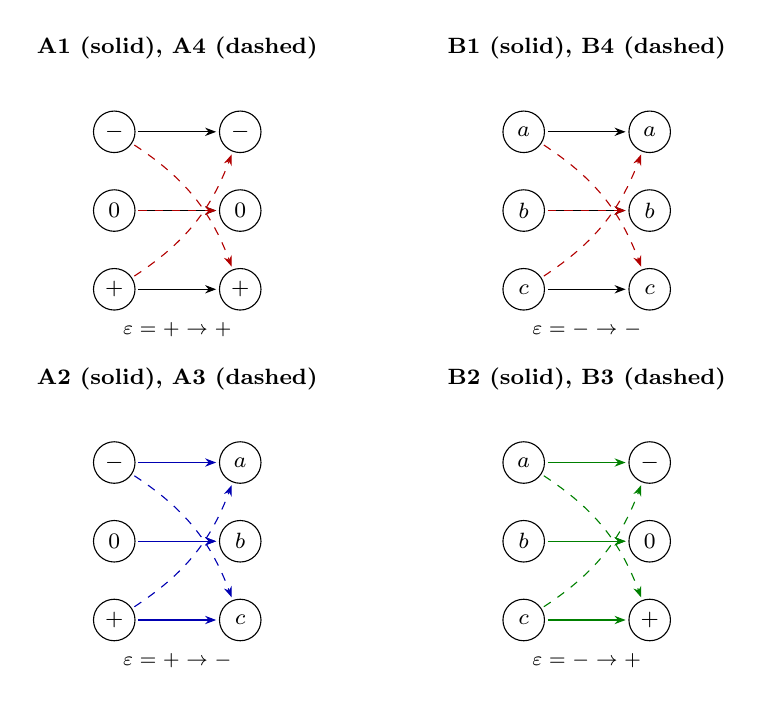
\begin{tikzpicture}[
  >={Stealth[length=4pt]},
  shorten >=1pt, shorten <=1pt,
  letter/.style={circle,draw=black,minimum size=15pt,inner sep=0pt,
                 font=\footnotesize},
  panellabel/.style={font=\footnotesize\bfseries,anchor=south},
  panel/.style={inner sep=2pt}]

% ============ Panel 1: A1 (identity on +) and A4 (swap on +) ============
\begin{scope}[xshift=0cm,yshift=0cm]
  \node[letter] (a1m) at (0,2)   {$-$};
  \node[letter] (a1z) at (0,1)   {$0$};
  \node[letter] (a1p) at (0,0)   {$+$};
  \node[letter] (a1m2) at (1.6,2) {$-$};
  \node[letter] (a1z2) at (1.6,1) {$0$};
  \node[letter] (a1p2) at (1.6,0) {$+$};
  % A1: identity (solid black)
  \draw[->] (a1m) -- (a1m2);
  \draw[->] (a1z) -- (a1z2);
  \draw[->] (a1p) -- (a1p2);
  % A4: swap (red dashed)
  \draw[->,red!70!black,dashed] (a1m) to[bend left=18] (a1p2);
  \draw[->,red!70!black,dashed] (a1p) to[bend right=18] (a1m2);
  \draw[->,red!70!black,dashed] (a1z) -- (a1z2);
  \node[panellabel] at (0.8,2.8) {A1 (solid), A4 (dashed)};
  \node[font=\scriptsize,anchor=north] at (0.8,-0.3) {$\varepsilon=+\to+$};
\end{scope}

% ============ Panel 2: B1 (identity on -) and B4 (swap on -) ============
\begin{scope}[xshift=5.2cm,yshift=0cm]
  \node[letter] (b1a) at (0,2)   {$a$};
  \node[letter] (b1b) at (0,1)   {$b$};
  \node[letter] (b1c) at (0,0)   {$c$};
  \node[letter] (b1a2) at (1.6,2) {$a$};
  \node[letter] (b1b2) at (1.6,1) {$b$};
  \node[letter] (b1c2) at (1.6,0) {$c$};
  % B1: identity (solid black)
  \draw[->] (b1a) -- (b1a2);
  \draw[->] (b1b) -- (b1b2);
  \draw[->] (b1c) -- (b1c2);
  % B4: swap (red dashed)
  \draw[->,red!70!black,dashed] (b1a) to[bend left=18]  (b1c2);
  \draw[->,red!70!black,dashed] (b1c) to[bend right=18] (b1a2);
  \draw[->,red!70!black,dashed] (b1b) -- (b1b2);
  \node[panellabel] at (0.8,2.8) {B1 (solid), B4 (dashed)};
  \node[font=\scriptsize,anchor=north] at (0.8,-0.3) {$\varepsilon=-\to-$};
\end{scope}

% ============ Panel 3: A2 (straight) and A3 (reversed), + -> - ============
\begin{scope}[xshift=0cm,yshift=-4.2cm]
  \node[letter] (a2m) at (0,2)   {$-$};
  \node[letter] (a2z) at (0,1)   {$0$};
  \node[letter] (a2p) at (0,0)   {$+$};
  \node[letter] (a2a2) at (1.6,2) {$a$};
  \node[letter] (a2b2) at (1.6,1) {$b$};
  \node[letter] (a2c2) at (1.6,0) {$c$};
  % A2: straight (solid blue)
  \draw[->,blue!70!black]        (a2m) -- (a2a2);
  \draw[->,blue!70!black]        (a2z) -- (a2b2);
  \draw[->,blue!70!black]        (a2p) -- (a2c2);
  % A3: reversed (blue dashed)
  \draw[->,blue!70!black,dashed] (a2m) to[bend left=18]  (a2c2);
  \draw[->,blue!70!black,dashed] (a2p) to[bend right=18] (a2a2);
  \draw[->,blue!70!black,dashed] (a2z) -- (a2b2);
  \node[panellabel] at (0.8,2.8) {A2 (solid), A3 (dashed)};
  \node[font=\scriptsize,anchor=north] at (0.8,-0.3) {$\varepsilon=+\to-$};
\end{scope}

% ============ Panel 4: B2 (straight) and B3 (reversed), - -> + ============
\begin{scope}[xshift=5.2cm,yshift=-4.2cm]
  \node[letter] (b2a) at (0,2)   {$a$};
  \node[letter] (b2b) at (0,1)   {$b$};
  \node[letter] (b2c) at (0,0)   {$c$};
  \node[letter] (b2m2) at (1.6,2) {$-$};
  \node[letter] (b2z2) at (1.6,1) {$0$};
  \node[letter] (b2p2) at (1.6,0) {$+$};
  % B2: straight (solid green)
  \draw[->,green!50!black]        (b2a) -- (b2m2);
  \draw[->,green!50!black]        (b2b) -- (b2z2);
  \draw[->,green!50!black]        (b2c) -- (b2p2);
  % B3: reversed (green dashed)
  \draw[->,green!50!black,dashed] (b2a) to[bend left=18]  (b2p2);
  \draw[->,green!50!black,dashed] (b2c) to[bend right=18] (b2m2);
  \draw[->,green!50!black,dashed] (b2b) -- (b2z2);
  \node[panellabel] at (0.8,2.8) {B2 (solid), B3 (dashed)};
  \node[font=\scriptsize,anchor=north] at (0.8,-0.3) {$\varepsilon=-\to+$};
\end{scope}

\end{tikzpicture}
\caption{The eight letter-shift maps $\varphi_X$ of
Table~\ref{tab:letter-maps}, grouped by sign change of
$\varepsilon$.  Each panel shows two sub-cases that share the
same source/target alphabets: solid arrows for the
\emph{straight-order} map, dashed arrows for the
\emph{reversed-order} map (a single transposition of the two
extremal letters).
\textbf{Top row}: same-sign maps ($\varepsilon$ unchanged) ---
A1/A4 act on $\mathcal{P}_+ \sim \{-,0,+\}$;
B1/B4 act on $\mathcal{P}_- \sim \{a,b,c\}$.
\textbf{Bottom row}: sign-flip maps ---
A2/A3 send $\mathcal{P}_+ \to \mathcal{P}_-$;
B2/B3 send $\mathcal{P}_- \to \mathcal{P}_+$.
In every panel the two middle letters ($0$ and $b$) are fixed.
This is the algebraic source of the bigram-filter invariance
of Lemma~\ref{lem:letter-maps}: the forbidden bigrams
$\mathcal{F}_+ = \{(-,+),(+,-)\}$ and
$\mathcal{F}_- = \{(a,c),(c,a)\}$ involve only the two extremal
letters of each alphabet, so they map to the corresponding pair
of forbidden bigrams under every $\varphi_X$.}
\label{fig:letter-maps}
\end{figure}

\begin{lemma}[Letter-shift invariance of the bigram filter]
\label{lem:letter-maps}
Let $\mathcal{F}_+ = \{(-, +), (+, -)\} \subset
\mathcal{P}_+ \times \mathcal{P}_+$ and
$\mathcal{F}_- = \{(a, c), (c, a)\} \subset
\mathcal{P}_- \times \mathcal{P}_-$ be the forbidden bigrams of
Theorem~\ref{thm:nindep-real}.  Then for every sub-case $X$,
\[
  (\varphi_X \times \varphi_X)\bigl(\mathcal{F}_{\varepsilon(X)}\bigr)
  \;=\; \mathcal{F}_{\varepsilon'(X)},
\]
where $\varepsilon(X), \varepsilon'(X) \in \{+, -\}$ are the parent
and child signs of sub-case~$X$.
\end{lemma}

\begin{proof}
Read off Table~\ref{tab:letter-maps}.  Sub-cases A1 and A4 act on
$\mathcal{P}_+$ as identity and $- \leftrightarrow +$ respectively;
both swap $\mathcal{F}_+$ to itself.  Sub-cases B1 and B4 act on
$\mathcal{P}_-$ as identity and $a \leftrightarrow c$; both swap
$\mathcal{F}_-$ to itself.  Sub-cases A2 and A3 send $\mathcal{P}_+
\to \mathcal{P}_-$ via $\{-,0,+\} \to \{a,b,c\}$ in straight or
reversed order; in either order the unordered image of $\{-,+\}$ is
$\{a, c\}$, so each ordered forbidden bigram of $\mathcal{F}_+$ maps
to an ordered forbidden bigram of $\mathcal{F}_-$.  The same holds
for B2 and B3 in the reverse direction.
\end{proof}

\begin{lemma}[Bigram-shift identity]
\label{lem:bigram-shift}
Let $\sigma = (\varepsilon, T) \in \mathcal{B}(d, n)$ and let
$\sigma' = (\varepsilon', T')$ be any admissible refinement of
$\sigma$ via sub-case $X$.  Then for every $1 \le j \le d-1$ with
$j + 2 \le d$,
\begin{equation}\label{eq:bigram-shift}
  \bigl(T'_{j+1},\, T'_{j+2}\bigr)
  \;=\; \bigl(\varphi_X(T_j),\, \varphi_X(T_{j+1})\bigr).
\end{equation}
In particular, if the interior bigram $(T_j, T_{j+1})$ lies in
$\mathcal{F}_\varepsilon$, then $(T'_{j+1}, T'_{j+2})$ lies in
$\mathcal{F}_{\varepsilon'}$.
\end{lemma}

\begin{proof}
Equation~\eqref{eq:bigram-shift} is~\eqref{eq:Tprime-i} applied at
$i = j+1$ and $i = j+2$, both of which lie in the range $i \ge 2$
where the formula $T'_i = f_X(T_{i-1})$ holds without modification.
The forbidden-bigram statement is then
Lemma~\ref{lem:letter-maps}.
\end{proof}

\subsection{Closedness of the filter under refinement}
\label{ssec:filter-closed}

We say that $\sigma = (\varepsilon, T) \in \mathcal{B}(d, n)$
\emph{passes the filter} of Theorem~\ref{thm:nindep-real} if
\textup{(}i\textup{)} no internal bigram $(T_j, T_{j+1})$,
$1 \le j \le d-1$, lies in $\mathcal{F}_\varepsilon$, and
\textup{(}ii\textup{)} when $\varepsilon = -$, the additional rule
\textup{(M2)} $\neg\,(T_1 = a \wedge T_d = b)$ holds.

\begin{proposition}[Filter is closed under admissible refinement]
\label{prop:filter-closed}
Let $\sigma \in \mathcal{B}(d, n)$ and let $\sigma'$ be any
admissible refinement of $\sigma$.  If the bigram clause
\textup{(i)} of the filter fails for $\sigma$ at an interior
position $j \le d - 2$, then it also fails for $\sigma'$ at position
$j + 1$.
\end{proposition}

\begin{proof}
By Lemma~\ref{lem:bigram-shift} the forbidden bigram at position
$(j, j+1)$ of $\sigma$ is sent by $\varphi_X \times \varphi_X$ to a
forbidden bigram at position $(j+1, j+2)$ of $\sigma'$, which is
again an interior position since $j + 2 \le d$.  By
Lemma~\ref{lem:letter-maps} the image bigram lies in
$\mathcal{F}_{\varepsilon'}$, so it falsifies the filter for
$\sigma'$.
\end{proof}

\subsection{Right-edge dead end: the bigram $(c, a)$}
\label{ssec:right-edge-ca}

The bigram $(c, a)$ occurs at the right edge of a candidate
$\sigma \in \mathcal{B}_-(d, n)$ when $T_{d-1} = 3n - 4$ and
$T_d = n - 2$.  Since $T_d \in \mathcal{Q}_- = \{n-2, 2n-3\} =
\{a, b\}$, the symmetric forbidden bigram $(a, c)$ never occurs at
the right edge, so $(c, a)$ is the only case left open by
Proposition~\ref{prop:filter-closed} on the $\mathcal{B}_-$ side.

\begin{lemma}[Right-edge $(c, a)$ has no admissible child]
\label{lem:right-edge-ca-dead}
Let $n \ge 3$ and let $\sigma = (-, T) \in \mathcal{B}_-(d, n)$ with
$T_{d-1} = 3n - 4$ and $T_d = n - 2$.  Then $\sigma$ has no
admissible refinement: for every digit pair $(k, l)$ with
$0 \le k, l \le n - 1$, the candidate
$\sigma' = (\varepsilon', T')$ defined by~\eqref{eq:eps-prime}--%
\eqref{eq:Tprime-i} fails the admissibility box of
Theorem~\ref{thm:bandt-explicit}.
\end{lemma}

\begin{proof}
There are four sub-cases B1--B4 according to the signs
$(\varepsilon_k, \varepsilon_l)$.  In each we evaluate
$T'_d$ via~\eqref{eq:Tprime-i} or, in the case $i = d$, the
admissibility constraint $|T'_d| \le n - 2$ (sign-$+I$ child) or
$T'_d \in \mathcal{Q}_- = \{n-2, 2n-3\}$ (sign-$-I$ child).

\smallskip\noindent\emph{B1} \textup{(}$\varepsilon_k = \varepsilon_l =
+1$, $\varepsilon' = -1$\textup{)}: $T'_d = T_{d-1} = 3n - 4$.
Admissibility on the $\mathcal{B}_-$ side requires
$T'_d \le 2n - 3$, but $3n - 4 > 2n - 3$ for $n \ge 2$.

\smallskip\noindent\emph{B2} \textup{(}$\varepsilon_k = -1$,
$\varepsilon_l = +1$, $\varepsilon' = +1$\textup{)}:
$T'_d = T_{d-1} - (2n - 3) = n - 1$.
Admissibility on the $\mathcal{B}_+$ side requires
$|T'_d| \le n - 2$, but $|n - 1| = n - 1 > n - 2$.

\smallskip\noindent\emph{B3} \textup{(}$\varepsilon_k = +1$,
$\varepsilon_l = -1$, $\varepsilon' = +1$\textup{)}:
$T'_d = (2n - 3) - T_{d-1} = -(n - 1)$.
Again $|T'_d| = n - 1 > n - 2$.

\smallskip\noindent\emph{B4} \textup{(}$\varepsilon_k = \varepsilon_l =
-1$, $\varepsilon' = -1$\textup{)}:
$T'_d = 2(2n - 3) - T_{d-1} = n - 2 \in \mathcal{Q}_-$, so the
$T'_d$-constraint is satisfied.  However, the $T'_1$-constraint
already excludes this sub-case for the given $T_d = n - 2$:
substituting $T_d = n - 2$ in~\eqref{eq:Tprime-1} gives
\[
  T'_1 \;=\; 2(n^2 - n - 1) - n(n - 2) \;=\; n^2 - 2,
\]
and admissibility on the $\mathcal{B}_-$ side requires
$T'_1 \le 4n - 6$, contradicting
$n^2 - 2 > 4n - 6 \iff (n - 2)^2 > 0$, true for $n \ge 3$.

\smallskip
In all four sub-cases the candidate $\sigma'$ leaves the
admissibility box, so $\sigma$ has no admissible refinement.
\end{proof}

\begin{corollary}\label{cor:right-edge-ca-unreal}
Every $\sigma \in \mathcal{B}_-(d, n)$ with right-edge bigram
$(c, a)$ is unreal.
\end{corollary}

\begin{proof}
A real neighbor $\sigma$ of $A$ admits an infinite chain of
admissible refinements $\sigma = \sigma_0 \to \sigma_1 \to \cdots$
\textup{(}see Section~\ref{sec:higherdim}\textup{)}.
Lemma~\ref{lem:right-edge-ca-dead} forces this chain to terminate
at $\sigma_0$, contradicting reality.
\end{proof}

\subsection{Bigram half of the filter}
\label{ssec:gap}

Combining Proposition~\ref{prop:filter-closed} \textup{(}interior
bigrams\textup{)} with Corollary~\ref{cor:right-edge-ca-unreal}
\textup{(}right-edge $(c, a)$\textup{)} yields the full easy
direction of the $\mathcal{B}_-$ filter as far as bigrams are
concerned: every interior or right-edge occurrence of $(a, c)$ or
$(c, a)$ in a candidate $\sigma \in \mathcal{B}_-(d, n)$ obstructs
reality, either directly \textup{(}right edge\textup{)} or by
forcing all descendants to inherit a forbidden bigram
\textup{(}interior, by induction on depth via
Proposition~\ref{prop:filter-closed}\textup{)}.  The same argument
applied to $\mathcal{B}_+$ uses Lemmas~\ref{lem:letter-maps}
\textup{(}A1, A4\textup{)} and the absence of any right-edge issue:
on the $\mathcal{B}_+$ side, $T_d = 0$ is forced, so the
right-edge bigram is always $(\cdot, 0)$ which is never in
$\mathcal{F}_+ = \{(-, +), (+, -)\}$.

\begin{proposition}[Bigram half of the filter]
\label{prop:bigram-half}
Let $n \ge 3$ and $d \ge 2$.  Every $\sigma \in \mathcal{B}(d, n)$
with a forbidden bigram \textup{(}from $\mathcal{F}_+$ or
$\mathcal{F}_-$ according to $\varepsilon$\textup{)} at any
position is unreal.
\end{proposition}

\begin{proof}
For interior bigrams $(j, j+1)$ with $j \le d - 2$,
Proposition~\ref{prop:filter-closed} produces a forbidden bigram in
every admissible descendant, so the unique infinite-orbit witness
of reality cannot exist.  For the right-edge bigram in
$\mathcal{B}_+$ the case is empty by the preceding paragraph.  For
the right-edge bigram in $\mathcal{B}_-$ \textup{(}only $(c, a)$ is
possible\textup{)}, Corollary~\ref{cor:right-edge-ca-unreal} closes
the case.
\end{proof}

\subsection{Endpoint dead end: the rule (M2)}
\label{ssec:m2}

The remaining ingredient of
Theorem~\ref{thm:nindep-real} is the asymmetric endpoint
rule: a candidate $\sigma = (-, T) \in \mathcal{B}_-(d, n)$ with
$T_1 = a$ and $T_d = b$ is unreal even when its bigram filter
passes.

\begin{lemma}[Endpoint dead end]
\label{lem:endpoint-dead}
Let $n \ge 3$ and $d \ge 2$.  Let
$\sigma = (-, T) \in \mathcal{B}_-(d, n)$ satisfy $T_1 = a$,
$T_d = b$.  Then every admissible refinement $\sigma'$ of $\sigma$
either fails the bigram filter of Theorem~\ref{thm:nindep-real}
or has the right-edge bigram $(c, a)$.  Consequently $\sigma$ is
unreal.
\end{lemma}

\begin{proof}
Throughout, $T_1 = n - 2$ and $T_d = 2n - 3$.

\smallskip\noindent\emph{Sub-case B1}
\textup{(}$\varepsilon_k = \varepsilon_l = +1$, $\varepsilon' =
-1$\textup{)}.
By the proof of Theorem~\ref{thm:bandt-explicit}, the
admissibility constraint at $T_d = 2n - 3$ forces $k + l = 2n - 4$
and $T'_1 = 3n - 4 = c$.  For $d \ge 3$, $T'_2 = \varphi_{B1}(T_1)
= a$, so $\sigma'$ has the interior bigram $(T'_1, T'_2) = (c, a)
\in \mathcal{F}_-$.  For $d = 2$, $T'_d = T'_2 = T_1 = a$, and the
child $(T'_1, T'_d) = (c, a)$ is the right-edge bigram of
Lemma~\ref{lem:right-edge-ca-dead}.

\smallskip\noindent\emph{Sub-case B2}
\textup{(}$\varepsilon_k = -1$, $\varepsilon_l = +1$, $\varepsilon'
= +1$\textup{)}.
The constraint at $T_d = 2n - 3$ forces $l = n - 2$ and $T'_1 = n
- 1 = +$, while the constraint $|T'_d| \le n - 2$ at $i = d$
forces $T'_d = 0$, i.e.\ $T_{d-1} = 2n - 3$.  For $d \ge 3$,
$T'_2 = \varphi_{B2}(T_1) = \varphi_{B2}(a) = -$, so $\sigma'$ has
the interior bigram $(T'_1, T'_2) = (+, -) \in \mathcal{F}_+$.
For $d = 2$ the constraint $T_{d-1} = T_1 = b$ is violated by
$T_1 = a$, so this sub-case is inadmissible.

\smallskip\noindent\emph{Sub-case B3}
\textup{(}$\varepsilon_k = +1$, $\varepsilon_l = -1$, $\varepsilon'
= +1$\textup{)}.
Symmetric to B2: $k = n - 2$, $T'_1 = -(n - 1) = -$, $T'_d = 0$
forces $T_{d-1} = 2n - 3$.  For $d \ge 3$, $T'_2 = \varphi_{B3}(a)
= +$, giving $(T'_1, T'_2) = (-, +) \in \mathcal{F}_+$.  For
$d = 2$ inadmissible by the same argument.

\smallskip\noindent\emph{Sub-case B4}
\textup{(}$\varepsilon_k = \varepsilon_l = -1$, $\varepsilon' =
-1$\textup{)}.
At $T_d = 2n - 3$, $T'_1 = n - 2 = a$, and the constraint
$T'_d \in \mathcal{Q}_-$ forces $T_{d-1} = 2n - 3$.  For $d \ge 3$,
$T'_2 = \varphi_{B4}(T_1) = \varphi_{B4}(a) = c$, giving
$(T'_1, T'_2) = (a, c) \in \mathcal{F}_-$.  For $d = 2$ the
constraint $T_{d-1} = T_1 = b$ is violated by $T_1 = a$,
inadmissible.

\smallskip
In every admissible sub-case, $\sigma'$ either contains a
forbidden interior bigram (and is unreal by
Proposition~\ref{prop:bigram-half}) or is the right-edge $(c, a)$
candidate (and is unreal by
Corollary~\ref{cor:right-edge-ca-unreal}).  Thus $\sigma$ has no
real refinement, so the infinite admissible orbit witnessing
reality cannot exist, and $\sigma$ is unreal.
\end{proof}

\begin{proposition}[Necessity half of the filter]
\label{prop:necessity}
Let $n \ge 3$ and $d \ge 2$.  Every $\sigma \in \mathcal{B}(d, n)$
that violates the filter of Theorem~\ref{thm:nindep-real} is
unreal.
\end{proposition}

\begin{proof}
A filter violation is either a forbidden bigram (handled by
Proposition~\ref{prop:bigram-half}) or, on the $\mathcal{B}_-$
side, the configuration $T_1 = a \wedge T_d = b$ (handled by
Lemma~\ref{lem:endpoint-dead}).
\end{proof}

\subsection{Hard direction: existence of an infinite orbit}
\label{ssec:hard-direction}

By the Bandt criterion~\cite{bandt1991,lau-ngai}
\textup{(}see also Section~\ref{sec:higherdim}\textup{)}, a
candidate $\sigma \in \mathcal{B}(d, n)$ is a real neighbor of
$C_n^{(d)}$ if and only if it admits an infinite chain
$\sigma = \sigma_0 \to \sigma_1 \to \sigma_2 \to \cdots$ of
admissible refinements.  The hypotheses of the criterion apply
here by the complete-residue tiling and OSC established in
Corollary~\ref{cor:comb-tile}, and by the finite Bandt-candidate
containment of Theorem~\ref{thm:bandt-explicit}.  Hence to
establish sufficiency of the
filter of Theorem~\ref{thm:nindep-real} it suffices to show
that the set of filter-passing candidates is \emph{forward
invariant} under admissible refinement: every filter-passing
$\sigma$ has at least one filter-passing admissible child.

\begin{lemma}[Filter-passing forward invariance]
\label{lem:forward-invariance}
Let $n \ge 3$ and $d \ge 1$, and let $\sigma \in \mathcal{B}(d, n)$
pass the filter of Theorem~\ref{thm:nindep-real}.  Then there
exists an admissible refinement $\sigma \to \sigma'$ with $\sigma'$
filter-passing.
\end{lemma}

\begin{proof}
We exhaust the parent according to $\varepsilon$ and the
last-coordinate data $(T_{d-1}, T_d)$ \textup{(}when $d \ge 2$;
the $d = 1$ case is handled at the end\textup{)}.  In each case
we exhibit a sub-case $X \in \{\textup{A1}, \ldots, \textup{B4}\}$
and digit indices $(k, l)$ for which $\sigma'$ is admissible, and
we verify that $\sigma'$ passes the filter.  Interior bigrams of
$\sigma'$ at positions $(j, j+1)$ with $j \ge 2$ are
$(\varphi_X(T_{j-1}), \varphi_X(T_j))$ by
Lemma~\ref{lem:bigram-shift}; since $\varphi_X$ maps
$\mathcal{F}_\varepsilon$ to $\mathcal{F}_{\varepsilon'}$ bijectively
by Lemma~\ref{lem:letter-maps}, these are non-forbidden whenever
the parent's interior bigrams are.  Thus we need only verify the
new bigram $(T'_1, T'_2) = (T'_1, \varphi_X(T_1))$ and, when
$\varepsilon' = -$, the rule \textup{(M2)}.

The finite choices used below are summarised in
Table~\ref{tab:forward-invariance-check}.  The subsequent
paragraphs verify admissibility and the new left-edge filter
condition in each row.

\begin{table}[ht]
\centering
\footnotesize
\caption{Forward-invariance choices for the filter-passing set.}
\label{tab:forward-invariance-check}
\begin{tabular}{@{}p{0.27\textwidth}p{0.25\textwidth}p{0.34\textwidth}@{}}
\toprule
Parent data & Chosen sub-case & Filter check for the child \\
\midrule
$\varepsilon=+$, $T_{d-1}=0$ & A1, $k=l$ & right shift; new bigram starts with $0$ \\
$\varepsilon=+$, $T_{d-1}=+$ & A3, $(k,l)=(n-2,n-1)$ & $T'_1=b$, so \textup{(M2)} fails in the antecedent \\
$\varepsilon=+$, $T_{d-1}=-$ & A2, $(k,l)=(n-1,n-2)$ & $T'_1=b$, same \textup{(M2)} check \\
$\varepsilon=-$, $T_d=a$ & B1, $k+l=n-3$ & $T'_1=b$ avoids both $\mathcal F_-$ and \textup{(M2)} \\
$\varepsilon=-$, $T_d=b$, $T_{d-1}\in\{a,b\}$ & B1, $k+l=2n-4$ & $T'_1=c$; parent \textup{(M2)} excludes $T_1=a$ \\
$\varepsilon=-$, $T_d=b$, $T_{d-1}=c$ & B4 & $T'_d=a$; parent \textup{(M2)} excludes $T_1=a$ \\
$d=1$ & B1 for $a\to b$, B4 for $b\to a$ & two-state forward-invariant set $\{a,b\}$ \\
\bottomrule
\end{tabular}
\end{table}

\smallskip\noindent\textbf{Macro-case $\varepsilon = +$.}
Then $T_d = 0$.

\emph{If $T_{d-1} = 0$}, choose sub-case~\textup{A1} with $k = l$
\textup{(}any value in $\{0, \ldots, n-2\}$; the child does not
depend on the common value\textup{)}.  Then~\eqref{eq:Tprime-1}
gives $T'_1 = (k - l)(n - 1) = 0$ and~\eqref{eq:Tprime-i} gives
$T'_i = T_{i-1}$ for $2 \le i \le d$, so the child is the
\emph{right shift}
\[
  \sigma' \;=\; (+,\, 0,\, T_1,\, T_2,\, \ldots,\, T_{d-1}),
\]
in particular $T'_d = T_{d-1} = 0$ and
$\sigma' \in \mathcal{B}_+(d, n)$ (since $\sigma \neq (I, 0)$
implies $T \neq 0$, hence $\sigma' \neq (I, 0)$).  The new bigram
$(T'_1, T'_2) = (0, \varphi_{\textup{A1}}(T_1)) = (0, T_1)$ has
first letter $0 \notin \{-, +\}$, so it is not in $\mathcal{F}_+$;
all other interior bigrams of $\sigma'$ are inherited from $\sigma$
through the shift and pass the filter by
Lemma~\ref{lem:bigram-shift}.

\emph{Termination of the right-shift orbit.}\ Iterating this choice
produces a sequence $\sigma = \sigma^{(0)} \to \sigma^{(1)} \to
\cdots$ in which each step shifts the last coordinate off (it was
$0$, hence the shift is admissible) and prepends $0$ on the left.
After at most $d$ such steps the rightmost non-zero entry of the
original $T$ has been shifted past position $d-1$, leaving
$\sigma^{(k)}$ with $T^{(k)}_{d-1} = T_{d-1-k}$ in $\{-, 0, +\}$.
Whenever $T^{(k)}_{d-1} \neq 0$ the next step switches to
sub-case~\textup{A2} or~\textup{A3} as analysed in the next two
paragraphs; whenever $T^{(k)}_{d-1} = 0$ another~\textup{A1} step
is applied.  Since $T \neq 0$ for $\sigma \in \mathcal{B}_+(d, n)$,
at least one entry $T_j$ is non-zero, so within $d$ steps the
orbit reaches an iterate with $T^{(k)}_{d-1} \neq 0$ and exits to
the non-trivial sub-cases.

\emph{If $T_{d-1} = +$} \textup{(}i.e.\ $T_{d-1} = n - 1$\textup{)},
choose sub-case~\textup{A3} with $k = n - 2$, $l = n - 1$.  Then
$T'_1 = (n-1)(n-k) - 1 = 2n - 3 = b$, $\varepsilon' = -1$, and
$T'_d = (2n - 3) - T_{d-1} = n - 2 = a$.  The new bigram
$(b, \varphi_{\textup{A3}}(T_1))$ has first letter $b$, which
cannot be the first letter of any pair in $\mathcal{F}_- =
\{(a, c), (c, a)\}$.  Rule \textup{(M2)} for the child: $T'_1 = b
\ne a$, so the antecedent fails.

\emph{If $T_{d-1} = -$}, symmetrically choose~\textup{A2} with
$k = n - 1$, $l = n - 2$: $T'_1 = (n-1)(n-l) - 1 = 2n - 3 = b$,
$T'_d = T_{d-1} + (2n - 3) = n - 2 = a$, and the argument is
identical.

\smallskip\noindent\textbf{Macro-case $\varepsilon = -$.}
Then $T_d \in \{a, b\}$, and the filter forces $(T_{d-1}, T_d)
\ne (c, a)$; moreover \textup{(M2)} forbids $(T_1, T_d) = (a, b)$.

\emph{If $T_d = a$} \textup{(}so $T_{d-1} \in \{a, b\}$\textup{)},
choose sub-case~\textup{B1} with $k + l = n - 3$, $\varepsilon_k =
\varepsilon_l = +1$ \textup{(}both digits $< n-1$, feasible for
$n \ge 3$\textup{)}.  Reading the B1 entry of
Theorem~\ref{thm:bandt-explicit} at $T_d = n - 2$ gives $T'_1 =
2n - 3 = b$.  \textup{(}The alternative B1 refinement with $k + l
= n - 2$ would yield $T'_1 = n - 2 = a$ and the new bigram $(a,
\varphi_{\textup{B1}}(T_1)) = (a, T_1)$; this can fall into
$\mathcal{F}_- = \{(a, c), (c, a)\}$ when $T_1 = c$, since
\textup{(M2)} on the parent imposes no constraint on $T_1$ when
$T_d = a$.  The choice $T'_1 = b$ avoids this and works for every
filter-passing parent.\textup{)}  Thus $T'_1 = b$, and $T'_d =
T_{d-1} \in \{a, b\} = \mathcal{Q}_-$, admissible.  The new bigram
$(b, T_1)$ has first letter $b$ and is not in $\mathcal{F}_-$.
Rule \textup{(M2)} for the child: $T'_1 = b \ne a$, antecedent
fails.

\emph{If $T_d = b$ and $T_{d-1} \in \{a, b\}$}, choose~\textup{B1}
with $k + l = 2n - 4$.  Then $T'_1 = 3n - 4 = c$, $T'_d = T_{d-1}
\in \{a, b\}$, admissible.  The new bigram $(c, T_1)$ is in
$\mathcal{F}_-$ only if $T_1 = a$; but \textup{(M2)} applied to
the parent forbids $T_1 = a$ when $T_d = b$, so $T_1 \in \{b, c\}$
and $(c, T_1) \in \{(c, b), (c, c)\} \not\subset \mathcal{F}_-$.
Rule \textup{(M2)} for the child: $T'_1 = c \ne a$.

\emph{If $T_d = b$ and $T_{d-1} = c$}, choose sub-case~\textup{B4}.
Then $T'_1 = 2(n^2 - n - 1) - nb = n - 2 = a$ and $T'_d =
2(2n - 3) - T_{d-1} = n - 2 = a$, admissible.  The new bigram
$(a, \varphi_{\textup{B4}}(T_1))$: by \textup{(M2)} on the parent,
$T_1 \ne a$, so $T_1 \in \{b, c\}$ and $\varphi_{\textup{B4}}(T_1)
\in \{b, a\}$.  Hence the bigram is $(a, b)$ or $(a, a)$, not in
$\mathcal{F}_-$.  Rule \textup{(M2)} for the child: $T'_d = a \ne
b$, antecedent fails.

\smallskip\noindent\textbf{Boundary case $d = 1$.}
$\mathcal{B}_+(1, n) = \emptyset$, so only $\mathcal{B}_-(1, n) =
\{a, b\}$ is relevant; both elements pass the filter trivially
\textup{(}there are no interior bigrams; \textup{(M2)} collapses
since $T_1 = T_d$ cannot be both $a$ and $b$\textup{)}.  The
refinement $a \to b$ is produced by~\textup{B1} with $k + l =
n - 3$ \textup{(}feasible for $n \ge 3$, giving $T'_1 = 2n - 3 =
b$\textup{)}; the refinement $b \to a$ is produced by~\textup{B4},
giving $T'_1 = n - 2 = a$ as computed in the previous case.  Both
children pass the filter, so $\{a, b\}$ is forward-invariant.
\end{proof}

\begin{proof}[Proof of Theorem~\ref{thm:nindep-real}]
Necessity is Proposition~\ref{prop:necessity}.  For sufficiency,
iterate Lemma~\ref{lem:forward-invariance}: any filter-passing
$\sigma$ has a filter-passing child $\sigma_1$, which in turn has
a filter-passing child $\sigma_2$, and so on, yielding an
infinite chain of admissible refinements.  By the Bandt
criterion~\cite{bandt1991,lau-ngai}, $\sigma$ is a real neighbor.
\end{proof}


\begin{thebibliography}{14}

\bibitem{akiyama-thuswaldner}
S.~Akiyama and J.\,M.~Thuswaldner,
A survey on topological properties of tiles related to number systems,
\emph{Geom.\ Dedicata}\ \textbf{109} (2004), 89--105.

\bibitem{bandt1991}
C.~Bandt,
Self-similar sets.~5. Integer matrices and fractal tilings of~$\R^n$,
\emph{Proc.\ Amer.\ Math.\ Soc.}\ \textbf{112} (1991), 549--562.

\bibitem{bandt-wang}
C.~Bandt and Y.~Wang,
Disk-like self-affine tiles in~$\R^2$,
\emph{Discrete Comput.\ Geom.}\ \textbf{26} (2001), 591--601.

\bibitem{baumgartel}
H.~Baumg\"artel,
\emph{Analytic Perturbation Theory for Matrices and Operators},
Operator Theory: Adv.\ Appl.\ \textbf{15},
Birkh\"auser, Basel, 1985.

\bibitem{loridant-luo-thuswaldner}
B.~Loridant, J.~Luo and J.\,M.~Thuswaldner,
Topology of crystallographic tiles,
\emph{Geom.\ Dedicata}\ \textbf{128} (2007), 113--144.

\bibitem{duvall-keesling-strichartz}
P.~Duvall, J.~Keesling and A.~Strichartz,
Hausdorff dimension of boundaries of self-similar tiles,
\emph{Indiana Univ.\ Math.\ J.}\ \textbf{44} (1995), 765--782.

\bibitem{falconer}
K.\,J.~Falconer,
\emph{Fractal Geometry: Mathematical Foundations and Applications}, 3rd~ed.,
Wiley, 2014.

\bibitem{grunbaum-shephard}
B.~Gr{\"u}nbaum and G.\,C.~Shephard,
\emph{Tilings and Patterns},
W.\,H.~Freeman, New York, 1987.

\bibitem{guthrie-nymann}
J.\,A.~Guthrie and J.\,E.~Nymann,
The topological structure of the set of subsums of an infinite
series,
\emph{Colloq.\ Math.}\ \textbf{55} (1988), 323--327.

\bibitem{hata}
M.~Hata,
On the structure of self-similar sets,
\emph{Japan J.\ Appl.\ Math.}\ \textbf{2} (1985), 381--414.

\bibitem{hutchinson}
J.\,E.~Hutchinson,
Fractals and self-similarity,
\emph{Indiana Univ.\ Math.\ J.}\ \textbf{30} (1981), 713--747.

\bibitem{ifstile}
D.~Mekhontsev,
IFStile: a tool for exploring iterated function systems,
software, \url{https://ifstile.com}, 2019--2026.

\bibitem{keesling}
J.~Keesling,
The boundaries of self-similar tiles in~$\R^n$,
\emph{Topology Appl.}\ \textbf{94} (1999), 195--205.

\bibitem{lagarias-wang}
J.\,C.~Lagarias and Y.~Wang,
Self-affine tiles in~$\R^n$,
\emph{Adv.\ Math.}\ \textbf{121} (1996), 21--49.

\bibitem{lau-ngai}
K.-S.~Lau and S.-M.~Ngai,
Multifractal measures and a weak separation condition,
\emph{Adv.\ Math.}\ \textbf{141} (1999), 45--96.

\bibitem{leung-lau}
K.-S.~Leung and K.-S.~Lau,
Disklikeness of planar self-affine tiles,
\emph{Trans.\ Amer.\ Math.\ Soc.}\ \textbf{359} (2007), 3337--3355.

\bibitem{mauldin-williams}
R.\,D.~Mauldin and S.\,C.~Williams,
Hausdorff dimension in graph directed constructions,
\emph{Trans.\ Amer.\ Math.\ Soc.}\ \textbf{309} (1988), 811--829.

\bibitem{moro-burke-overton-1997}
J.~Moro, J.\,V.~Burke and M.\,L.~Overton,
On the Lidskii--Vishik--Lyusternik perturbation theory for
eigenvalues of matrices with arbitrary Jordan structure,
\emph{SIAM J.\ Matrix Anal.\ Appl.}\ \textbf{18} (1997), 793--817.

\bibitem{ngai-tang}
S.-M.~Ngai and T.-M.~Tang,
Topology of connected self-similar tiles in the plane,
\emph{Topology Appl.}\ \textbf{150} (2005), 139--155.

\bibitem{oeis-A213667}
OEIS Foundation Inc.,
Sequence~A213667,
\emph{The On-Line Encyclopedia of Integer Sequences},
\url{https://oeis.org/A213667}, 2026.

\bibitem{oeis-A265278}
OEIS Foundation Inc.,
Sequence~A265278,
\emph{The On-Line Encyclopedia of Integer Sequences},
\url{https://oeis.org/A265278}, 2026.

\bibitem{oeis-A293004}
OEIS Foundation Inc.,
Sequence~A293004,
\emph{The On-Line Encyclopedia of Integer Sequences},
\url{https://oeis.org/A293004}, 2026.

\bibitem{scheicher-thuswaldner}
K.~Scheicher and J.\,M.~Thuswaldner,
Neighbours of self-affine tiles in lattice tilings,
\emph{Fractals in Graz 2001} (P.~Grabner and W.~Woess, eds.),
Trends Math., Birkh{\"a}user, 2003, pp.~241--262.

\end{thebibliography}

\end{document}
